% Options for packages loaded elsewhere
% Options for packages loaded elsewhere
\PassOptionsToPackage{unicode}{hyperref}
\PassOptionsToPackage{hyphens}{url}
\PassOptionsToPackage{dvipsnames,svgnames,x11names}{xcolor}
%
\documentclass[
  number,
  review,
  onecolumn]{elsarticle}
\usepackage{xcolor}
\usepackage[lmargin=2.5cm,rmargin=2.5cm,tmargin=3cm,bmargin=3cm]{geometry}
\usepackage{amsmath,amssymb}
\setcounter{secnumdepth}{5}
\usepackage{iftex}
\ifPDFTeX
  \usepackage[T1]{fontenc}
  \usepackage[utf8]{inputenc}
  \usepackage{textcomp} % provide euro and other symbols
\else % if luatex or xetex
  \usepackage{unicode-math} % this also loads fontspec
  \defaultfontfeatures{Scale=MatchLowercase}
  \defaultfontfeatures[\rmfamily]{Ligatures=TeX,Scale=1}
\fi
\usepackage{lmodern}
\ifPDFTeX\else
  % xetex/luatex font selection
\fi
% Use upquote if available, for straight quotes in verbatim environments
\IfFileExists{upquote.sty}{\usepackage{upquote}}{}
\IfFileExists{microtype.sty}{% use microtype if available
  \usepackage[]{microtype}
  \UseMicrotypeSet[protrusion]{basicmath} % disable protrusion for tt fonts
}{}
\makeatletter
\@ifundefined{KOMAClassName}{% if non-KOMA class
  \IfFileExists{parskip.sty}{%
    \usepackage{parskip}
  }{% else
    \setlength{\parindent}{0pt}
    \setlength{\parskip}{6pt plus 2pt minus 1pt}}
}{% if KOMA class
  \KOMAoptions{parskip=half}}
\makeatother
% Make \paragraph and \subparagraph free-standing
\makeatletter
\ifx\paragraph\undefined\else
  \let\oldparagraph\paragraph
  \renewcommand{\paragraph}{
    \@ifstar
      \xxxParagraphStar
      \xxxParagraphNoStar
  }
  \newcommand{\xxxParagraphStar}[1]{\oldparagraph*{#1}\mbox{}}
  \newcommand{\xxxParagraphNoStar}[1]{\oldparagraph{#1}\mbox{}}
\fi
\ifx\subparagraph\undefined\else
  \let\oldsubparagraph\subparagraph
  \renewcommand{\subparagraph}{
    \@ifstar
      \xxxSubParagraphStar
      \xxxSubParagraphNoStar
  }
  \newcommand{\xxxSubParagraphStar}[1]{\oldsubparagraph*{#1}\mbox{}}
  \newcommand{\xxxSubParagraphNoStar}[1]{\oldsubparagraph{#1}\mbox{}}
\fi
\makeatother


\usepackage{longtable,booktabs,array}
\usepackage{calc} % for calculating minipage widths
% Correct order of tables after \paragraph or \subparagraph
\usepackage{etoolbox}
\makeatletter
\patchcmd\longtable{\par}{\if@noskipsec\mbox{}\fi\par}{}{}
\makeatother
% Allow footnotes in longtable head/foot
\IfFileExists{footnotehyper.sty}{\usepackage{footnotehyper}}{\usepackage{footnote}}
\makesavenoteenv{longtable}
\usepackage{graphicx}
\makeatletter
\newsavebox\pandoc@box
\newcommand*\pandocbounded[1]{% scales image to fit in text height/width
  \sbox\pandoc@box{#1}%
  \Gscale@div\@tempa{\textheight}{\dimexpr\ht\pandoc@box+\dp\pandoc@box\relax}%
  \Gscale@div\@tempb{\linewidth}{\wd\pandoc@box}%
  \ifdim\@tempb\p@<\@tempa\p@\let\@tempa\@tempb\fi% select the smaller of both
  \ifdim\@tempa\p@<\p@\scalebox{\@tempa}{\usebox\pandoc@box}%
  \else\usebox{\pandoc@box}%
  \fi%
}
% Set default figure placement to htbp
\def\fps@figure{htbp}
\makeatother





\setlength{\emergencystretch}{3em} % prevent overfull lines

\providecommand{\tightlist}{%
  \setlength{\itemsep}{0pt}\setlength{\parskip}{0pt}}



 
\usepackage[]{natbib}
\bibliographystyle{elsarticle-num}


\newpageafter{author}
\usepackage{lineno}
\makeatletter
\@ifpackageloaded{float}{}{\usepackage{float}}
\floatstyle{plain}
\@ifundefined{c@chapter}{\newfloat{figsupp}{h}{lofigsupp}}{\newfloat{figsupp}{h}{lofigsupp}[chapter]}
\floatname{figsupp}{Figure S}
\newcommand*\quartofigsuppref[1]{Figure \hyperref[#1]{S\ref{#1}}}
\@ifpackageloaded{caption}{}{\usepackage{caption}}
\DeclareCaptionLabelFormat{quartofigsuppreflabelformat}{#1#2}
\captionsetup[figsupp]{labelformat=quartofigsuppreflabelformat}
\newcommand*\listoffigsupps{\listof{figsupp}{List of Supplementary Figures}}
\makeatother
\makeatletter
\@ifpackageloaded{float}{}{\usepackage{float}}
\floatstyle{plain}
\@ifundefined{c@chapter}{\newfloat{tabsupp}{h}{lotabsupp}}{\newfloat{tabsupp}{h}{lotabsupp}[chapter]}
\floatname{tabsupp}{Table S}
\newcommand*\quartotabsuppref[1]{Table \hyperref[#1]{S\ref{#1}}}
\@ifpackageloaded{caption}{}{\usepackage{caption}}
\DeclareCaptionLabelFormat{quartotabsuppreflabelformat}{#1#2}
\captionsetup[tabsupp]{labelformat=quartotabsuppreflabelformat}
\newcommand*\listoftabsupps{\listof{tabsupp}{List of Supplementary Tabless}}
\makeatother
\makeatletter
\@ifpackageloaded{float}{}{\usepackage{float}}
\floatstyle{plain}
\@ifundefined{c@chapter}{\newfloat{figmain}{h}{lofigmain}}{\newfloat{figmain}{h}{lofigmain}[chapter]}
\floatname{figmain}{Figure}
\newcommand*\listoffigmains{\listof{figmain}{List of Article Figuress}}
\makeatother
\makeatletter
\@ifpackageloaded{float}{}{\usepackage{float}}
\floatstyle{plain}
\@ifundefined{c@chapter}{\newfloat{tabmain}{h}{lotabmain}}{\newfloat{tabmain}{h}{lotabmain}[chapter]}
\floatname{tabmain}{Table}
\newcommand*\listoftabmains{\listof{tabmain}{List of Article Tabless}}
\makeatother
\makeatletter
\@ifpackageloaded{caption}{}{\usepackage{caption}}
\AtBeginDocument{%
\ifdefined\contentsname
  \renewcommand*\contentsname{Table of contents}
\else
  \newcommand\contentsname{Table of contents}
\fi
\ifdefined\listfigurename
  \renewcommand*\listfigurename{List of Figures}
\else
  \newcommand\listfigurename{List of Figures}
\fi
\ifdefined\listtablename
  \renewcommand*\listtablename{List of Tables}
\else
  \newcommand\listtablename{List of Tables}
\fi
\ifdefined\figurename
  \renewcommand*\figurename{Figure}
\else
  \newcommand\figurename{Figure}
\fi
\ifdefined\tablename
  \renewcommand*\tablename{Table}
\else
  \newcommand\tablename{Table}
\fi
}
\@ifpackageloaded{float}{}{\usepackage{float}}
\floatstyle{ruled}
\@ifundefined{c@chapter}{\newfloat{codelisting}{h}{lop}}{\newfloat{codelisting}{h}{lop}[chapter]}
\floatname{codelisting}{Listing}
\newcommand*\listoflistings{\listof{codelisting}{List of Listings}}
\makeatother
\makeatletter
\makeatother
\makeatletter
\@ifpackageloaded{caption}{}{\usepackage{caption}}
\@ifpackageloaded{subcaption}{}{\usepackage{subcaption}}
\makeatother
\journal{Proceedings of the Royal Society B - Biological Sciences}
\usepackage{bookmark}
\IfFileExists{xurl.sty}{\usepackage{xurl}}{} % add URL line breaks if available
\urlstyle{same}
\hypersetup{
  pdftitle={Why do birds use green nest material? A systematic review and meta-analysis of experiments},
  pdfauthor={Shreya Dimri; Tuba Rizvi; Júlio M.G. Segovia; Meinolf Ottensmann; Alfredo Sánchez-Tójar},
  colorlinks=true,
  linkcolor={blue},
  filecolor={Maroon},
  citecolor={Blue},
  urlcolor={Blue},
  pdfcreator={LaTeX via pandoc}}


\setlength{\parindent}{6pt}
\begin{document}

\begin{frontmatter}
\title{Why do birds use green nest material? A systematic review and
meta-analysis of experiments}
\author[1]{Shreya Dimri%
\corref{cor1}%
}
 \ead{shreya.dimri@uni-bielefeld.de} 
\author[1]{Tuba Rizvi%
%
}

\author[1]{Júlio M.G. Segovia%
%
}

\author[2]{Meinolf Ottensmann%
%
}

\author[1]{Alfredo Sánchez-Tójar%
%
}


\affiliation[1]{organization={Department of Evolutionary Biology,
Bielefeld University, Germany},,postcodesep={}}
\affiliation[2]{organization={Department of Animal Behaviour, Bielefeld
University, Germany},,postcodesep={}}

\cortext[cor1]{Corresponding author}





        
\begin{abstract}
Many animals construct nests. Nests are often considered extended
phenotypes that shape survival and reproduction beyond the builder's
body. Birds are key examples of nest builders, and many add fresh green
plant material to their nests. Yet, the adaptive value of this behaviour
remains debated. Non-mutually exclusive hypotheses propose roles in
courtship signalling, parasite defence, or direct enhancement of
offspring condition. Here, we conducted a pre-registered systematic
review and meta-analysis of 28 experimental studies (published and
unpublished), spanning seven bird species and 274 effect sizes, to test
whether green nest material influences fitness, and to evaluate the
competing functional explanations. Our synthesis shows that while green
nest material can enhance avian fitness, this effect depends on the
fitness proxy used, and its functional role remains unresolved. The
strongest predictor was experimental design, strongly influencing the
outcomes, challenging the role of aromatic compounds in the fitness
benefits of green nest material. Our meta-analysis supports the
importance of green nest material on fitness, but calls for more
research to elucidate its mechanisms.
\end{abstract}





\end{frontmatter}
    
\linenumbers


\section{Introduction}\label{introduction}

Nest and nest-building are fundamental across a diverse range of
animals, including arthropods (e.g., ants, spiders), mammals (e.g.,
platypus, rodents), and perhaps more famously, birds. Nests provide
structural support for eggs, parents, and offspring, and protect them
against predators and other environmental pressures, and are thus key to
reproductive success and survival
\citep{hansell2000, mainwaring2014, deeming2023}. Most birds use organic
plant materials such as twigs, branches, grass, and moss to build their
nests. Some even incorporate inorganic items, including mud, stones,
feathers, snake skins and anthropogenic materials like plastic and
cigarette butts
\citep{sergio2011, suárez-rodríguez2013, jagiello2023, sheard2024}. The
latter are considered non-structural additions and suggest that nests
are more than just physical shelters; they can be complex tools shaped
by both natural and sexual selection for multiple functions. Indeed,
nests can play a key role in sexual display, and features such as nest
size have been shown to act as sexually selected signals of parental
quality in several bird species \citep[e.g.,][]{moreno1994, hoi1996},
even interspecifically by brood parasites \citep{soler1995}.
Nest-building behaviour is increasingly recognised as an expression of
the extended phenotype (reviewed by \citep{moreno2012}), and phylogeny
has been shown to be an important factor explaining nest morphology
\citep{perez2023}. Yet, despite hundreds of scientific articles studying
nests and nesting behaviour in birds being published each year, much
remains unknown.

An intriguing nesting behaviour observed in some bird species is the
addition of fresh, often aromatic, plant material to the nest. This
green nest material (hereafter \emph{GNM}) often corresponds to leaves,
sprigs, herbs and branches, and is typically added from the start of
nest building until egg laying, although some species like the blue tit
(\emph{Cyanistes caeruleus}) keep adding it after that. Contrary to the
structural nest materials (e.g., twigs, mud), GNM is selected from a
small, non-random subset of local flora
\citep{clark1985, petit2002, garrido-bautista2023}. The selected plants
often possess high levels of aromatic volatile compounds (commonly used
by songbirds; \citep{mennerat2009b}) or secondary metabolites such as
oils and resins (commonly used by raptors; \citep{ontiveros2007}). GNM
is unlikely to be gathered opportunistically, and collecting these
uncommon plants and replenishing them, sometimes over weeks, requires
extra time and, in some cases, flying outside one's territory
\citep{mennerat2009}. Thus, the general costs associated with
nest-building \citep{mainwaring2013}, and the additional effort, time
and energy devoted to add these non-structural materials, suggest an
adaptive function of GNM.

Multiple hypotheses have been proposed to explain the adaptive function
of GNM (reviewed in \citep{dubiec2013}; \citep{scott-baumann2015}).
First, the courtship hypothesis suggests that (mostly) males use GNM as
visual or olfactory signals to attract females and/or advertise nest
site occupancy to other males (e.g., \citep{eens1993};
\citep{gwinner1997}; \citep{brouwer2004}), particularly in
cavity-nesting species where visual cues inside the nest are limited.
For instance, the seminal study of \citep{kessel1957} showed that male
European starlings (\emph{Sturnus vulgaris}) carry fresh plant material
to their nests while singing and displaying to females. Subsequent
studies in European and spotless starlings (\emph{Sturnus unicolor})
supported this view by showing that females often prefer nests with
fresh GNM, and that unpaired males conspicuously deliver GNM during
courtship, stopping right after the onset of egg laying
\citep{brouwer2004, veiga2006}. Additionally, males increase the
addition of GNM in the presence of potential mates \citep{eens1993}.
Altogether, these studies offered support for the courtship hypothesis,
which was later extended to explain GNM addition solely by females in
blue tits, suggesting that GNM might serve as a sexually selected signal
of female quality \citep{tomás2013}.

Second, the most widely tested hypothesis is the nest protection
hypothesis, which proposes that the volatile compounds in GNM reduce the
amount of parasites and pathogens in the nests, enhancing offspring
survival. This hypothesis was first suggested in a comparative study in
raptors (Falconiformes) that provided only indirect evidence by
comparing nest reuse, diet composition and GNM presence
\citep{wimberger1984}. Soon after, a preference for GNM containing
insect-repellent and antimicrobial volatiles was experimentally
confirmed in European starlings and suggested three key criteria for
evaluating the nest protection hypothesis (i.e., selective plant use,
bioactive chemical properties and demonstrable adaptive benefits;
\citep{clark1985}{]}. Observational and experimental studies on raptors
\citep{ontiveros2007, dykstra2009} and passerines
\citep{lafuma2001, dawson2004, mennerat2009b, quiroga2012} have shown
mixed results. In some cases, GNM was shown to improve offspring
condition without reducing the amount of parasites in the nests
\citep{gwinner2000}, leading to the development of the drug hypothesis.
This alternative hypothesis suggests that the volatiles present in GNM
directly enhance offspring immune function and/or health independent of
parasite or pathogen control\citep{gwinner2000, mennerat2009a}. While
both the nest protection and drug hypotheses suggest that GNM enhances
offspring survival, the drug hypothesis attributes this effect to a
pharmacological mechanism, whereas the nest protection hypothesis
emphasises parasite and pathogen repellency. Importantly, these two
hypotheses are not mutually exclusive, and their potential effects on
offspring survival are difficult to disentangle.

Last, several additional functional hypotheses of GNM that do not refer
to its aromatic (i.e., volatiles and secondary metabolites) properties
have also been proposed. These include benefits such as enhancing the
crypticity of the nest \citep{skutch1957}, providing insulation or sun
protection for eggs and offspring \citep{mertens1977}, or simply
fulfilling a structural function \citep{lyons1987}. However, these
alternative functional roles have received little support or attention.

Despite decades of research, abundant observational and experimental
studies, and two crucial narrative reviews
\citep{dubiec2013, scott-baumann2015}, we still do not know the overall
adaptive significance of GNM, its generality across bird species, and
the relative importance of each of the suggested functions. Given that
nest building is widespread across taxa, including but not limited to
birds, and is increasingly recognised as an expression of the extended
phenotype, a quantitative synthesis of this field is both timely and has
potentially far-reaching implications.~

To address this gap, we conducted a pre-registered systematic review and
meta-analysis of experiments testing the effect of GNM on various
fitness proxies across birds. Our meta-analysis explicitly evaluates the
overall evidence for the adaptive significance of GNM, as well as
assesses the relative importance of the main suggested hypotheses: the
courtship hypothesis and parental care hypothesis (i.e., a combination
of both the nest protection and drug hypotheses). In addition, we tested
potential moderators that might explain the observed context-dependency
(i.e., high heterogeneity among effect sizes). Specifically, we tested
whether the effect of GNM varied depending on the experimental design
used, the timing of GNM addition, the focal species studied, the
category of fitness proxy investigated (e.g.~morphological,
reproductive, etc.), and the type of parasite. Our meta-analysis of
experimental studies is the first quantitative synthesis testing the
causal relationship between GNM and fitness across birds.

\section{Methods}\label{methods}

\subsection{Registration and
reporting}\label{registration-and-reporting}

We pre-registered our study protocol on the Open Science Framework
\citep{dimri2024} prior to exploring or analysing the data. The
pre-registration details our objectives, a priori hypotheses and
predictions, methods and planned data analyses. Unless stated otherwise,
we adhered to the registered protocol. We followed the PRISMA-EcoEvo
guidelines \citep{odea2021} for reporting this study
(\quartotabsuppref{tabsupp-checklist};
\quartofigsuppref{figsupp-prisma-flowchart}). All resources associated
with this study, including data and code, are available at
{[}\url{https://github.com/shreyadimri/Green_Nest_Material}{]} (insert
Zenodo citation later).

\subsection{Information source and
search}\label{information-source-and-search}

We conducted a systematic search on Web of Science Core Collection and
Scopus on the 7th of September, 2022 (see update below). The keyword
search query was designed as a three-block query including terms related
to our treatment of interest ((``green*'' OR ``herb*'' OR ``aromatic*'')
AND ``nest*''), population of interest (``bird*'' OR ``aves'' OR
``avian'' OR ``ornithol*'' OR ``passerine*'' OR ``passeriform*'' OR
``songbird*'' OR list of all bird genera) and to limit the search
results to experimental studies only (``experiment*'' OR
``manipulat*''). The complete search strings tailored to each specific
platform are provided in \quartofigsuppref{figsupp-string}. Although our
search string only included keywords in English, we planned to screen
any study in English, Spanish, Portuguese and Hindi, but found studies
only in English. We searched through titles, abstracts and keywords with
no restrictions on publication date or study type. We validated our
search using an initial library of 15 relevant articles that we had
previously identified (\quartofigsuppref{figsupp-own-library}), ensuring
all were retrieved. Additionally, we used the R package `litsearchr'
v1.0.0 \citep{grames2019}, which did not yield any new relevant terms,
confirming our queries. After removing 152 duplicates using the R
package `revtools' v0.4.1 \citep{westgate2019}, we identified 383 unique
records.

\subsection{Eligibility criteria}\label{eligibility-criteria}

All titles and abstracts were equally allocated and screened
independently by at least two screeners (SD, TR, JMGS) using the R
package `revtools' following a pre-designed decision tree with all
inclusion/exclusion criteria (\quartofigsuppref{figsupp-decision-tree}).
We included all studies on birds that experimentally manipulated the GNM
(both aromatics and non-aromatic). Forty articles passed the
title-and-abstract screening and were further evaluated during the
full-text screening, where each article was independently screened by a
single screener (SD, TR, JMGS), with another screener verifying the
procedure. We used the same criteria as above
(\quartofigsuppref{figsupp-decision-tree}) with an additional evaluation
of whether the variable of interest in the article was in our list of
fitness proxies of interest
(\quartofigsuppref{figsupp-fitness-proxies}). Twenty-two aarticles
passed the full-text screening and were, thus, eligible for our
meta-analysis. All conflicts in screening decisions (1\% for
title-and-abstract screening, and none for full-text screening) were
resolved through discussion.

We updated our systematic literature search by repeating our search on
the 12th of August, 2024, and found 53 unique articles after removing 13
duplicates. Only one observer (SD) performed both screenings using the
same decision trees as before
(\quartofigsuppref{figsupp-decision-tree}), and found one additional
eligible article for our meta-analysis. Lastly, we identified three
additional eligible articles recommended by two colleagues. In all, 26
published articles were eligible for our meta-analysis, but we also
obtained two additional unpublished studies (more details below and in
\quartofigsuppref{figsupp-prisma-flowchart}).

\subsection{Data extraction}\label{data-extraction}

The data of each article were extracted by one of three authors (SD, TR,
JMGS), with another screener verifying the procedure, and four authors
(SD, TR, JMGS, AST) collectively discussing and revising unclear cases.
We prioritised extracting primary data (i.e., measures of central
tendency, variance and sample size) from text and tables, or, if that
was not possible, from figures (e.g., boxplots) using the R package
`metaDigitise' v1.0.1 \citep{pick2018}. If primary data were not
available, we extracted inferential statistics such as t and F values or
contingency tables to transform them into effect sizes (see below).
Last, if the previous steps failed but the article had openly archived
data, we calculated the means, standard deviations and sample sizes from
each group ourselves (n = 4 studies).

We extracted the means, variances and sample sizes for each
control-treatment comparison. Depending on the experimental design of
each study, controls included non-aromatic materials (e.g., grass or
moss), smaller amounts of aromatic material, no added material, or
removal of material added by birds; whereas treatments consisted of
aromatic material added by authors, birds, or both. We coded these
comparisons in our moderator `experimental design' as non-aromatic GNM
vs.~aromatic GNM, or no added GNM vs.~aromatic GNM. Another experimental
design used in some studies compared nests with experimentally added
non-aromatic GNM to nests without any added GNM or in which GNM added by
the birds was removed by the authors. In these cases, the non-aromatic
GNM was considered the treatment, and we coded these as non-aromatic GNM
vs.~no added GNM in our moderator `experimental design' (n = 3 studies).
Importantly, our conclusions remained robust to the exclusion of these
effect sizes (\quartotabsuppref{tabsupp-SA-intercept}), so we kept this
category in our dataset, and the moderator `experimental design' was
tested in subsequent meta-regressions. A fourth experimental design
compared enhanced supplementation of GNM by the authors (i.e., authors +
birds) to birds alone (n = 2). This experimental design represents a
fundamentally different contrast focused on potential additive effects
of GNM and makes the assumption that a GNM effect is indeed present;
therefore, we excluded it from the meta-regression using the
`experimental design' moderator. In studies where three groups were
compared (n = 5), we extracted all possible pairwise comparisons, and
accounted for (shared-group) non-independence in our analyses (more
below).

For each study, we also extracted information related to the study
subjects (bird species, geographical location of the study population),
the methodology of the study (fitness proxy measured) and the source
from which we extracted data (e.g., figures, tables, raw data files,
supplementary materials). We categorised the fitness proxies measured
into 6 broad categories: physiology, morphology, reproduction,
behaviour, parasite and pathogenic load, and phenology. For studies
testing whether GNM affects the number of parasites or pathogens found
in offspring and/or nests, we categorised them into arthropods or
microorganisms. For a complete list of variables extracted, see
\quartofigsuppref{figsupp-variables} . During data extraction, we
encountered some traits (e.g., WBC ratio, parent mass; 15 effect sizes,
n = 5 studies) that we did not include in any of our analyses because it
was unclear from the study and our own judgement how these traits
related to fitness (see \quartofigsuppref{figsupp-excluded-proxies} for
the list and reasons of exclusion).

We contacted four corresponding authors to obtain missing data (e.g.,
non-reported results, missing sample sizes). All four authors responded
to our email, but only two provided the data as requested; one did not
have the data any more, and one did not give a conclusive response.
Additionally, to locate grey literature (e.g., unpublished data), we
wrote to the corresponding author(s) of all the 22 articles that passed
full-text screening to ask for any potential unpublished data that could
be included in our meta-analysis using a standardised email template
(\quartofigsuppref{figsupp-email}). One author provided data for an
unpublished study on blue tits (see description in
\quartofigsuppref{figsupp-unpublished-study}), and one of us (MO)
provided data for an unpublished study on common buzzards (\emph{Buteo
buteo}).

\subsection{Effect size calculation}\label{effect-size-calculation}

Using the means, standard deviations and sample sizes for each
control-treatment pairwise comparison, we calculated two effect sizes: a
log response ratio (lnRR) and a standardised mean difference with
heteroskedasticity correction (SMDH), using the escalc function (measure
= `ROM' and `SMDH', respectively, vtype = `LS') in the R package
`metafor' v4.8-0 \citep{metafor}. We specified the treatment group as
the numerator and the control group as the denominator for lnRR, and
treatment minus control for SMDH, such that positive values indicate a
`fitness' increase in the treatment group. In cases such as measures of
parasite load or prevalence, laying or hatching dates, courtship time,
or scab score, the effect size sign was inverted before analysis to
ensure that a positive value consistently meant an increase in fitness
regardless of fitness proxy (i.e., to ensure comparability across effect
sizes). SMDH could only be calculated when there were enough data points
in both treatment and control groups to estimate the pooled variance;
specifically, when the degrees of freedom (i.e., n1+n2−2) were greater
than 1. There were nine effect sizes from one) study that did not
fulfill that requirement, which we then excluded from the dataset.

For the few cases for which we could not extract means and variances but
inferential statistics such as t and F values, we estimated SMD values
(k = 4, n = 2) using the equations provided by \citep{thehand2019}. For
dichotomous variables (e.g., number of successful nests, k = 4, n = 2),
we calculated the log odds ratio (lnOR) using the `escalc' function
(measure=OR) from `metafor' and subsequently converted it to SMD using
equations from \citep{thehand2019}. Since lnRR cannot be calculated from
inferential statistics, dichotomous variables, or traits including zero
or negative values (k = 7), the number of effect sizes included in the
lnRR subset (k = 259, n = 28) is smaller than that of SMDH (k = 274, n =
28).

When calculating each effect size's associated sampling variance,
whenever possible, we used the number of nests in each group over the
number of individuals as the sample size to account for genetic
relatedness non-independence. In cases where the same control or
treatment group was used in multiple comparisons, sample sizes were
adjusted before calculating effect sizes by dividing them by the number
of times each group was used in a comparison to account for shared group
non-independence. For cases where the authors of an original article
reported a statistically non-significant difference between two groups
but without providing numerical values (k = 16, n = 2), we assigned zero
as the effect size for that comparison and imputed its sampling variance
using the missing-case approach described in \citep{nakagawa2022} for
lnRR, and \(\frac{n_1+n_2}{n_1×n_2}\) for SMDH \citep{lajeunesse2013}.

\subsection{Data analysis}\label{data-analysis}

We performed all analyses in R v4.5.1 \citep{R-version}. All multilevel
meta-analytical models and meta-regressions were fitted using `metafor'
v4.8-0 \citep{metafor}. Sampling variances were modelled as
variance-covariance matrices assuming a 0.5 correlation (ρ) between
sampling variances from the same study \citep{noble2017} using the
`vcalc' function from `metafor' (see Supplementary Appendix
\quartofigsuppref{figsupp-correlation} for sensitivity analyses using
different values of \emph{ρ}).

We originally considered the following levels of non-independence for
our analyses: multiple effect sizes collected from~ (a) same study
(Paper ID), (b) bird species (Species ID), (c) geographical locations
(Population ID), (d) sub-populations within the same location
(Experiment ID; e.g., birds studied at the same location for multiple
years), (e) groups of individuals within a population (Group ID; e.g.,
males and females in a population, first clutch and second clutch), and
(f) repeated measurement of the same trait for the same individuals
(Repeated trait ID; e.g., chick mass on day 7, 14 and 21). In the end,
our random effect structure deviated from our pre-registration since,
initially, we had pre-registered the inclusion of Experiment ID and
Repeated trait ID, but not Population ID. However, Experiment ID and
Group ID were almost indistinguishable, so we decided to leave out the
one with lesser resolution (i.e.~Experiment ID). Additionally, few
effect sizes were measured repeatedly, making Repeated trait ID almost
identical to Observation ID (\quartofigsuppref{figsupp-random-effect}),
so we excluded Repeated trait ID. Last, we decided to add Population ID
since we noticed after extracting the data, but before any analyses,
that several studies were performed in the same geographical locations.
Therefore, unless stated otherwise, we fitted the following random
effects in all our models to account for non-independence: Paper ID,
Group ID, Species ID, Population ID and an observation-level random
effect (Observation ID).

\textbf{Meta-analytic mean and hypotheses}: To estimate the effect of
GNM on fitness across birds, we fitted two separate sets of models for
each effect size: lnRR and SMD(H). First, we fitted multilevel
intercept-only meta-analytical models to test the overall effect of GNM
on fitness estimates, its uncertainty and heterogeneity. We used the
`rma.mv' function from the `metafor' package (method = `REML' and test =
`t' for calculating the test statistics and confidence intervals for the
moderators). We excluded traits for which their link with fitness is
debated in the literature (e.g., sex ratio, testosterone levels) from
our main analysis, but conducted a sensitivity analysis including these
traits to test the robustness of our results
(\quartotabsuppref{tabsupp-SA-intercept}; k = 21 , n = 8). For all
intercept-only models, we estimated the total amount of absolute
heterogeneity (\(σ^2\); i.e., the total variation not explained by
sampling error), its sources or relative heterogeneity (\(I^2\)),
mean-standardised metric (CVH2) and variance-mean-standardised metric of
heterogeneity (M2) following the pluralistic approach suggested by
\citep{yang2024a} .

To test the relative importance of the two main functional hypotheses
suggested for GNM, that is, the courtship and the parental care
hypothesis, which combines the nest protection and drug hypotheses, we
ran a multilevel meta-regression including the moderator `hypothesis'
(levels: courtship, parental care, both). For all meta-regressions, we
estimated \(R_{marginal}^2\), which corresponds to the percentage of
heterogeneity explained by the moderators \citep{nakagawa2012}. Unless
stated otherwise, all meta-regressions correspond to unimoderator
meta-regressions.

\textsubscript{Source:
\href{https://shreyadimri.github.io/Green_Nest_Material/manuscript_GNM.qmd.html}{Article
Notebook}}

\textbf{Exploratory meta-regressions:} We performed additional
pre-registered multilevel meta-regressions for which we did not have
clear directional predictions. To understand the effect of type of
experimental design (i.e., whether the authors compared non-aromatic
vs.~aromatic, no added material vs.~aromatic, no added material
vs.~non-aromatic), we ran a meta-regression with the type of
`experimental design' as the moderator. To test the effect of time of
addition of GNM on fitness (levels: before egg hatching, after egg
hatching, continuously throughout the nesting phase), we ran a
meta-regression with `time of addition of GNM' as the moderator. We also
ran a meta-regression using `bird species' as the moderator (levels:
Buteo buteo, Cyanistes caeruleus, Passer cinnamomeus, Parus major,
Sturnus unicolor, Sturnus vulgaris, Tachycineta bicolor) to understand
if and how the effect of GNM on fitness might differ among species.
Furthermore, we explored the effect of GNM on fitness depending on the
`category of fitness proxy' studied (levels: behaviour, morphology,
parasite and pathogenic load, phenology, physiology, reproduction) using
a meta-regression with the fitness proxy category as the moderator.
Last, for the subset focusing on parasites and pathogens (k = 90, n =
16)), we ran a meta-regression with the `type of parasite' as the
moderator (levels: arthropod, micro-organism).~

In addition, we performed three additional pre-registered multilevel
meta-regressions to explore the potential threats to the internal
validity of each study on our conclusions (i.e., Risk of Bias or RoB)
following recommendations in \citep{culina2025} . We evaluated the
effects of (1) blinding (whether outcome assessors were blinded to the
experimental group), (2) random assignment to treatment, and (3) partial
reporting (whether all measured outcomes were completely reported or
only a subset). For each RoB category, we coded studies (levels: yes,
no) and included each category as a moderator in a meta-regression run
separately for both lnRR and SMD(H).

\textbf{Publication Bias Test:} Publication bias occurs when a subset of
research findings, most often statistically non-significant ones, are
less likely to be published or published later \citep{Jennisons2013}.
There are two types of publication biases that are commonplace in
ecology and evolutionary biology: small-study and decline effects
\citep{yang2023}. We tested them for both lnRR and SMD(H) separately,
following \citep{nakagawa2022a}. To test for small-study effects, we ran
a multilevel meta-regression using the `square-root of the inverse of
the effective sample size' as the moderator (i.e.,
\(\sqrt{(n_1+n_2)/ (4n_1n_2)}\)) To test for decline effects (also known
as time-lag bias; \citep{sanchez-tojar2018}), we ran a multilevel
meta-regression using `year of publication' (mean-centered) as the
moderator.

\section{Results}\label{results}

We obtained 274 effect sizes from a total of 28 studies conducted on 7
species across 17 geographical locations
(Figure\ref{figmain-distribution}). About 81\% of the effect sizes came
from only three bird species (Cyanistes caeruleus, k = 77; Sturnus
unicolor, k = 60; Sturnus vulgaris, k = 86). Our dataset included 2
unpublished studies (k = 18), with the remaining studies being published
between 1988 and 2024. The mean ±standard deviation number of effect
sizes per study was 9.8 ± 6.4 (median: 8.5 range: 2--24) and the mean
effective sample size (i.e., the number of nests/individuals per effect
size after accounting for shared-group non-independence) was 32.3 ±31.1
(median: 22.0, range: 3--210; 31 data points had a sample size of less
than 5 nests in each group).

\begin{figmain}

\centering{

\pandocbounded{
\includegraphics[keepaspectratio]{figures/Figure_Distribution.png}}

}

\caption{\label{figmain-distribution}\textbf{Geographical distribution
of the 17 study populations included in a meta-analysis testing the
adaptive value of green nest material in birds.} Point size reflects the
number of effect sizes coming from the location (range: 3--34), and
colour denotes species (see legend), with an inset zooming in on a dense
cluster of data points.}

\end{figmain}%

\subsection{Meta-analytic mean}\label{meta-analytic-mean}

Both lnRR and SMD(H) intercept-only multilevel meta-analyses showed an
average increase in fitness estimates in nests with an experimental
increase in GNM compared to control nests; however, the overall effect
was only statistically significant for SMD(H).~

First, lnRR showed an average statistically non-significant increase in
fitness estimates of 1.9\% in nests with an experimental increase in GNM
(Figure\ref{figmain-mean-effect} A; lnRR = 0.019, 95\% CI: {[}-0.012,
0.050{]}, 95\% PI: {[}-0.281, 0.319{]}, p-value = 0.223, k = 238, n =
26) but heterogeneity among effect sizes was high. Total raw
heterogeneity (\(\sigma^2\)) was 0.023 (\emph{Q} = 2277.7, p \textless{}
0.001), the measures of relative
(\emph{I\textsuperscript{2}\textsubscript{total}} = 98.6\%) and
standardised heterogeneity (CVH2\textsubscript{total} = 63.59;
M2\textsubscript{total~=} 0.98) all suggested high heterogeneity across
effect sizes, exceeding the 75th percentile of empirically derived
estimates from meta-analyses in ecology and evolution \citep{yang2024a}.

Second, SMD(H) showed an average statistically significant increase in
fitness estimates in nests with an experimental increase of GNM
(Figure\ref{figmain-mean-effect} B; SMD(H) = 0.179, 95\% CI: {[}0.048,
0.310{]}, 95\% PI: {[}-0.829, 1.188{]}, p-value = 0.008, k = 253, n =
26), but heterogeneity among effect sizes was moderate to high. Total
raw heterogeneity (\(\sigma^2\)) was 0.258 (\emph{Q} = 1114.7, p
\textless{} 0.001), relative heterogeneity was smaller compared to that
of lnRR (\emph{I\textsuperscript{2}\textsubscript{total}} = 66.1\%) and
the standardised heterogeneity metrics (CVH2\textsubscript{total} = 8.02
; M2\textsubscript{total~=} 0.89) lay between the 50th and 75th
percentile of empirically derived estimates \citep{yang2024a}.

The overall results and their conclusions were robust to several
sensitivity analyses. First, we fitted a pre-registered bivariate
multilevel meta-analytic model including both effect sizes as response
variables (lnRR = -0.015, p-value = 0.624 and SMD(H) = 0.250 , p-value =
0.069). In addition, we ran several sensitivity analyses to test the
robustness of the overall results to the: (i) inclusion of traits for
which their relationship with fitness was debated in the literature
(non-pre-registered); (ii) removal of effect sizes that were originally
reported as simply statistically non-significant and we assumed them to
be zero (non-pre-registered); (iii) both (i) and (ii)
(non-pre-registered); (iv) removal of effect sizes from non-aromatic
vs.~aromatic experimental design (non-pre-registered); (v) removal of
effect sizes from non-aromatic vs.~no added material experimental design
(non-pre-registered); (vi) removal of effect sizes that were calculated
by transforming inferential statistics (pre-registered); (vii) removal
of effect sizes that failed the Geary's Test for lnRR
(non-pre-registered); (viii) removal of unpublished data
(non-pre-registered); and (ix) use of different values of correlation
(ρ) between sampling variance for variance-covariance matrix
(pre-registered). The number of effect sizes included in those
sensitivity analyses ranged from 182 to 274, and the conclusions
remained largely the same \quartotabsuppref{tabsupp-SA-intercept}.

\begin{figmain}

\centering{

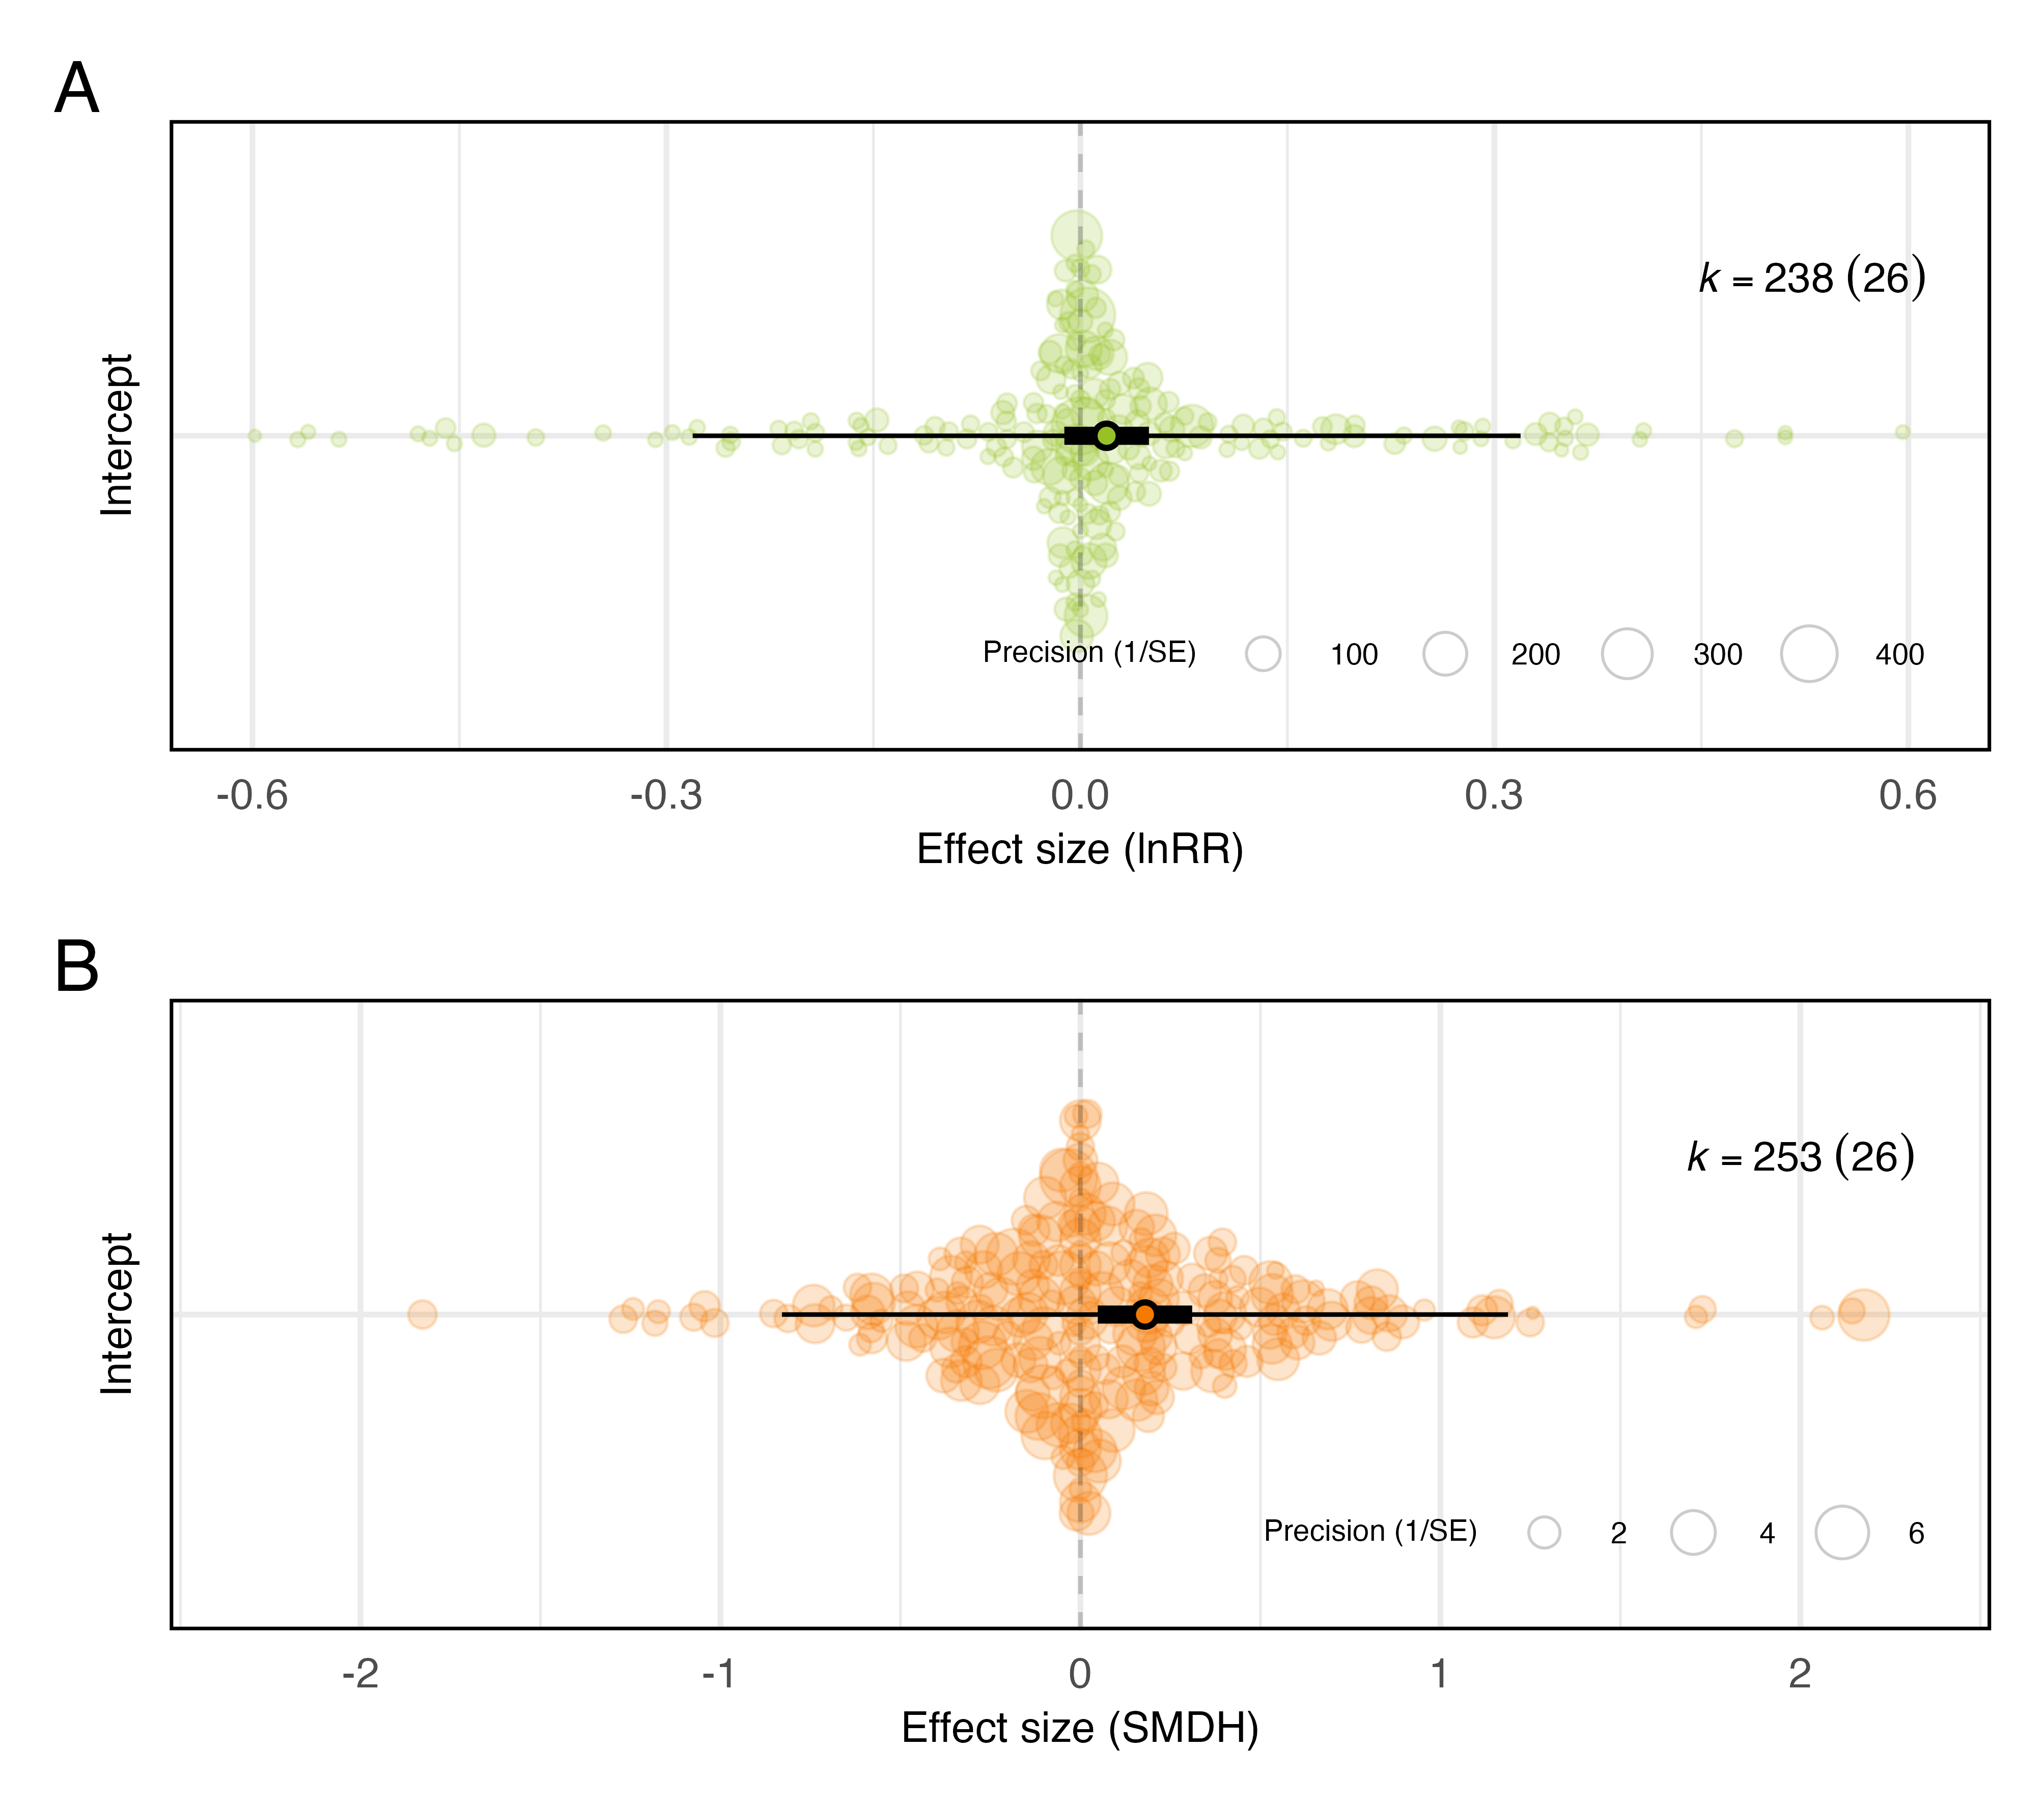
\includegraphics[width=0.9\linewidth,height=\textheight,keepaspectratio]{figures/Figure_overall_effect_crop.png}

}

\caption{\label{figmain-mean-effect}Overall effect of green nest
material on all fitness proxies combined. The meta-analytic mean (black
circle) with 95\% confidence intervals (thicker bars) and prediction
intervals (thinner bars) are shown along with the data points (coloured
circles) scaled by precision (inverse of standard error). Results are
shown as an orchard plot for the intercept-only model (A) using log
response ratio (lnRR), and (B) standardised mean difference (SMD(H)). k:
number of effect sizes (number of studies is shown in the brackets).
X-axes are truncated for legibility, which partially explains any
apparent asymmetry (complete figures in Section
\quartofigsuppref{figsupp-overall}).}

\end{figmain}%

\subsection{Functional hypotheses}\label{functional-hypotheses}

Our multilevel meta-regressions found no clear support for either of the
two main hypotheses proposed in the literature
(Figure\ref{figmain-hypothesis}). The estimates for the courtship
hypothesis (lnRR\textsubscript{courtship} = 0.039, 95\% CI: {[}-0.172,
0.250{]}, 95\% PI: {[}-0.329, 0.407{]}, p-value = 0.716, k = 8, n = 2;
SMD(H)\textsubscript{courtship} = 0.171, 95\% CI: {[}-0.360, 0.702{]},
95\% PI: {[}-0.964, 1.305{]}, p-value = 0.527, k = 8, n = 2), and the
nest protection and drug hypothesis (i.e., ``parental care hypothesis'')
(lnRR\textsubscript{parental\_care} = -0.010, 95\% CI: {[}-0.065,
0.045{]}, 95\% PI: {[}-0.316, 0.296{]}, p-value = 0.716, k = 106, n =
19; SMD(H)\textsubscript{parental\_care} = 0.109, 95\% CI: {[}-0.060,
0.278{]}, 95\% PI: {[}-0.908, 1.126{]}, p-value = 0.204, k = 115, n =
19) were statistically non-significant. However, about half of all
effect sizes could not be unequivocally assigned to only one hypothesis,
so our meta-regression contained a third category that combined both.
This category showed an average positive increase in fitness estimates
in nests with an experimental increase of GNM, but the effect was only
statistically significant for SMD(H) (lnRR\textsubscript{both} = 0.028,
95\% CI: {[}-0.006, 0.062{]}, 95\% PI: {[}-0.275, 0.331{]}, p-value =
0.110, k = 124, n = 22; SMD(H)\textsubscript{both} = 0.231, 95\% CI: {[}
0.079, 0.382{]}, 95\% PI: {[}-0.784, 1.245{]}, p-value = 0.003, k = 130,
n = 23). None of the three categories differed statistically
significantly from each other (\({p-value}_{lnRR)}\) \textgreater{}
0.211 and \({p-value}_{SMD(H)}\) \textgreater{} 0.178 in all cases), and
the moderator explained little heterogeneity (\(R^2_{marginal(lnRR)}\)=
1.6\% and \(R^2_{marginal(SMD(H))}\)= 1.4\%).

\begin{figmain}

\centering{

\pandocbounded{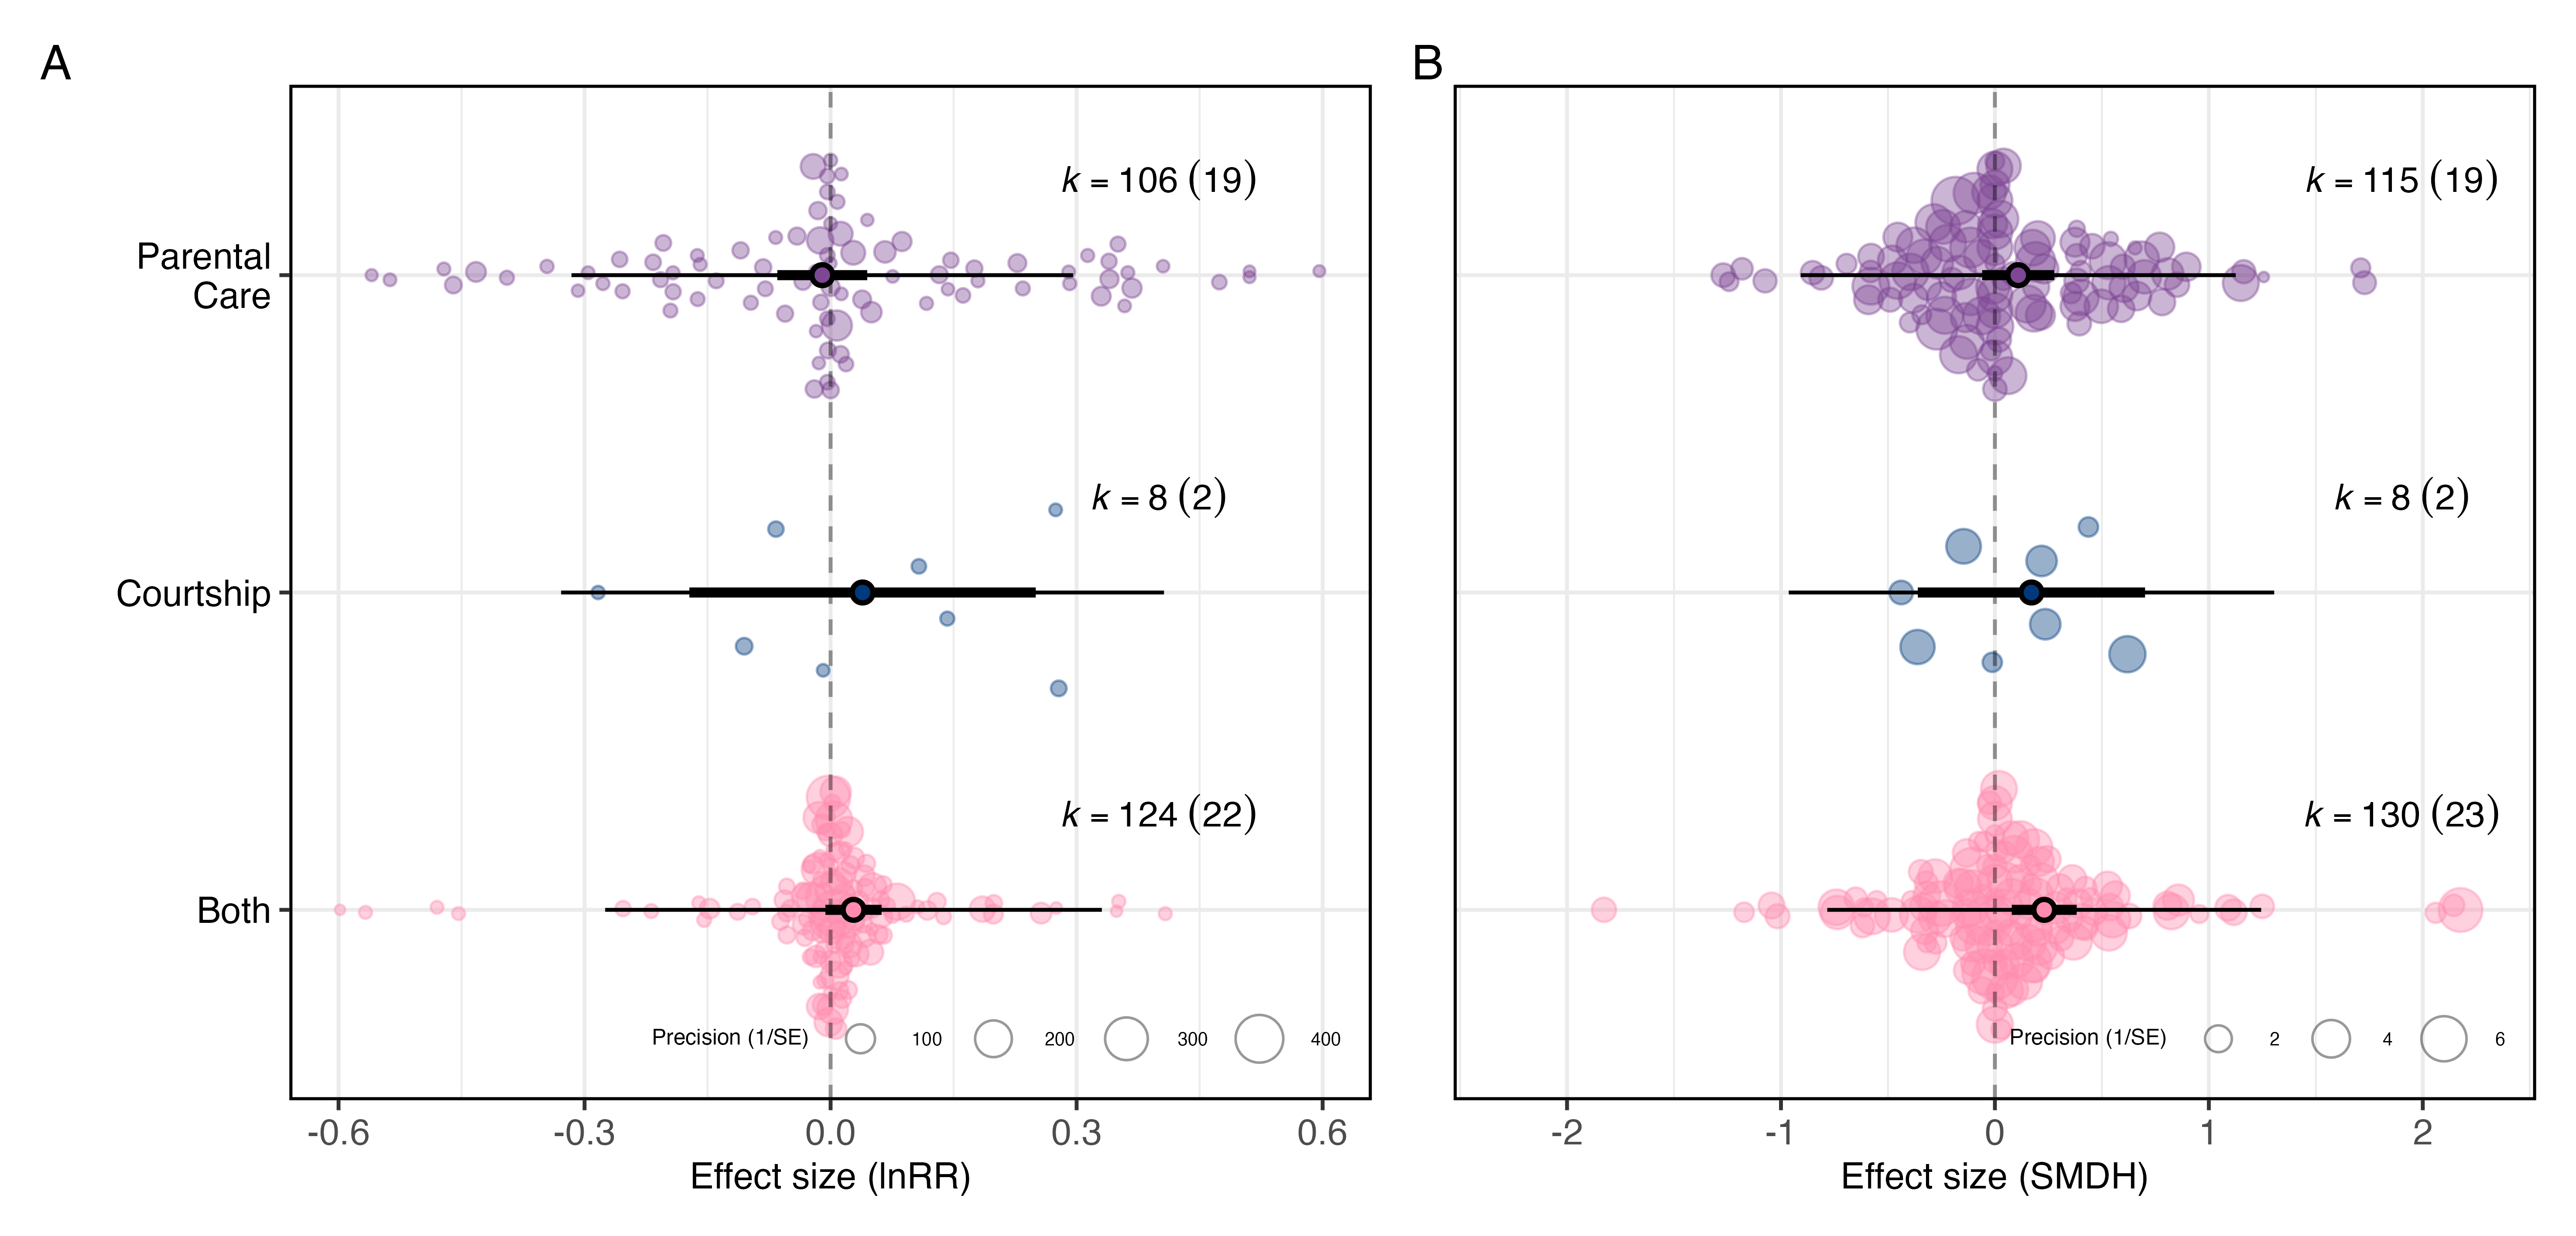
\includegraphics[keepaspectratio]{figures/Figure_hypothesis_crop.png}}

}

\caption{\label{figmain-hypothesis}There is no clear evidence to favour
either the courtship or the parental care hypothesis as drivers of
potential fitness benefits of green nest material. Orchard plot of the
multilevel meta-regression for (A) log response ratio (lnRR) and (B)
standardised mean difference (SMD(H)). Mean estimates (black circles),
95\% confidence intervals (thicker bars), and prediction intervals
(thinner bars) are shown along with the individual data points
(transparently coloured circles) scaled by precision (inverse of
standard error). k: number of effect sizes (number of studies is shown
in the brackets). X-axes are truncated for legibility, which partially
explains any apparent asymmetry (complete figures in Section
\quartofigsuppref{figsupp-hypothesis}.}

\end{figmain}%

\subsection{Exploratory
meta-regressions}\label{exploratory-meta-regressions}

First, the overall effect of GNM on fitness estimate differed largely
depending on the experimental design used
(Figure\ref{figmain-design-time}A,B). The overall effect size for the
comparison between no added material and aromatic GNM was positive and
statistically significant (lnRR\textsubscript{no-material-vs-aromatic} =
0.111, 95\% CI: {[} 0.021, 0.200{]}, 95\% PI: {[}-0.225, 0.446{]},
p-value = 0.016, k = 90, n = 12 and
SMD(H)\textsubscript{no-material-vs-aromatic} = 0.712, 95\% CI: {[}
0.309, 1.114{]}, 95\% PI: {[}-0.826, 2.250{]}, p-value = 0.001, k = 94,
n = 12{]}, whereas, the comparison between non-aromatic GNM and aromatic
GNM was small and statistically non-significant
(Table\ref{tabmain-MLMR}). The comparison between no added material and
non-aromatic GNM, was negative and, although based on only 3 studies,
statistically significantly for lnRR
(lnRR\textsubscript{no-material-vs-non-aromatic} = -0.349, 95\% CI:
{[}-0.504, -0.195{]}, 95\% PI: {[}-0.708, 0.009{]}, p-value
\textless0.001, k = 10, n = 3;Table\ref{tabmain-MLMR}). ~All levels
differed statistically significantly from each other except one
(\({p-value}_{lnRR}\) \textless{} 0.004 and \({p-value}_{SMD(H)}\)
\textless{} 0.001 in all cases, except~
\({SMD(H)}_{no-material-vs-aromatic}\)
vs.~\({SMD(H)}_{no-material-vs-non-aromatic}\) p-value = 0.140), and the
moderator experimental design explained a large proportion of
heterogeneity, indicating its great importance
(\(R^2_{marginal(lnRR)}\)= 27.8\% and \(R^2_{marginal(SMD(H))}\)=
24.4\%).

\begin{figmain}

\centering{

\pandocbounded{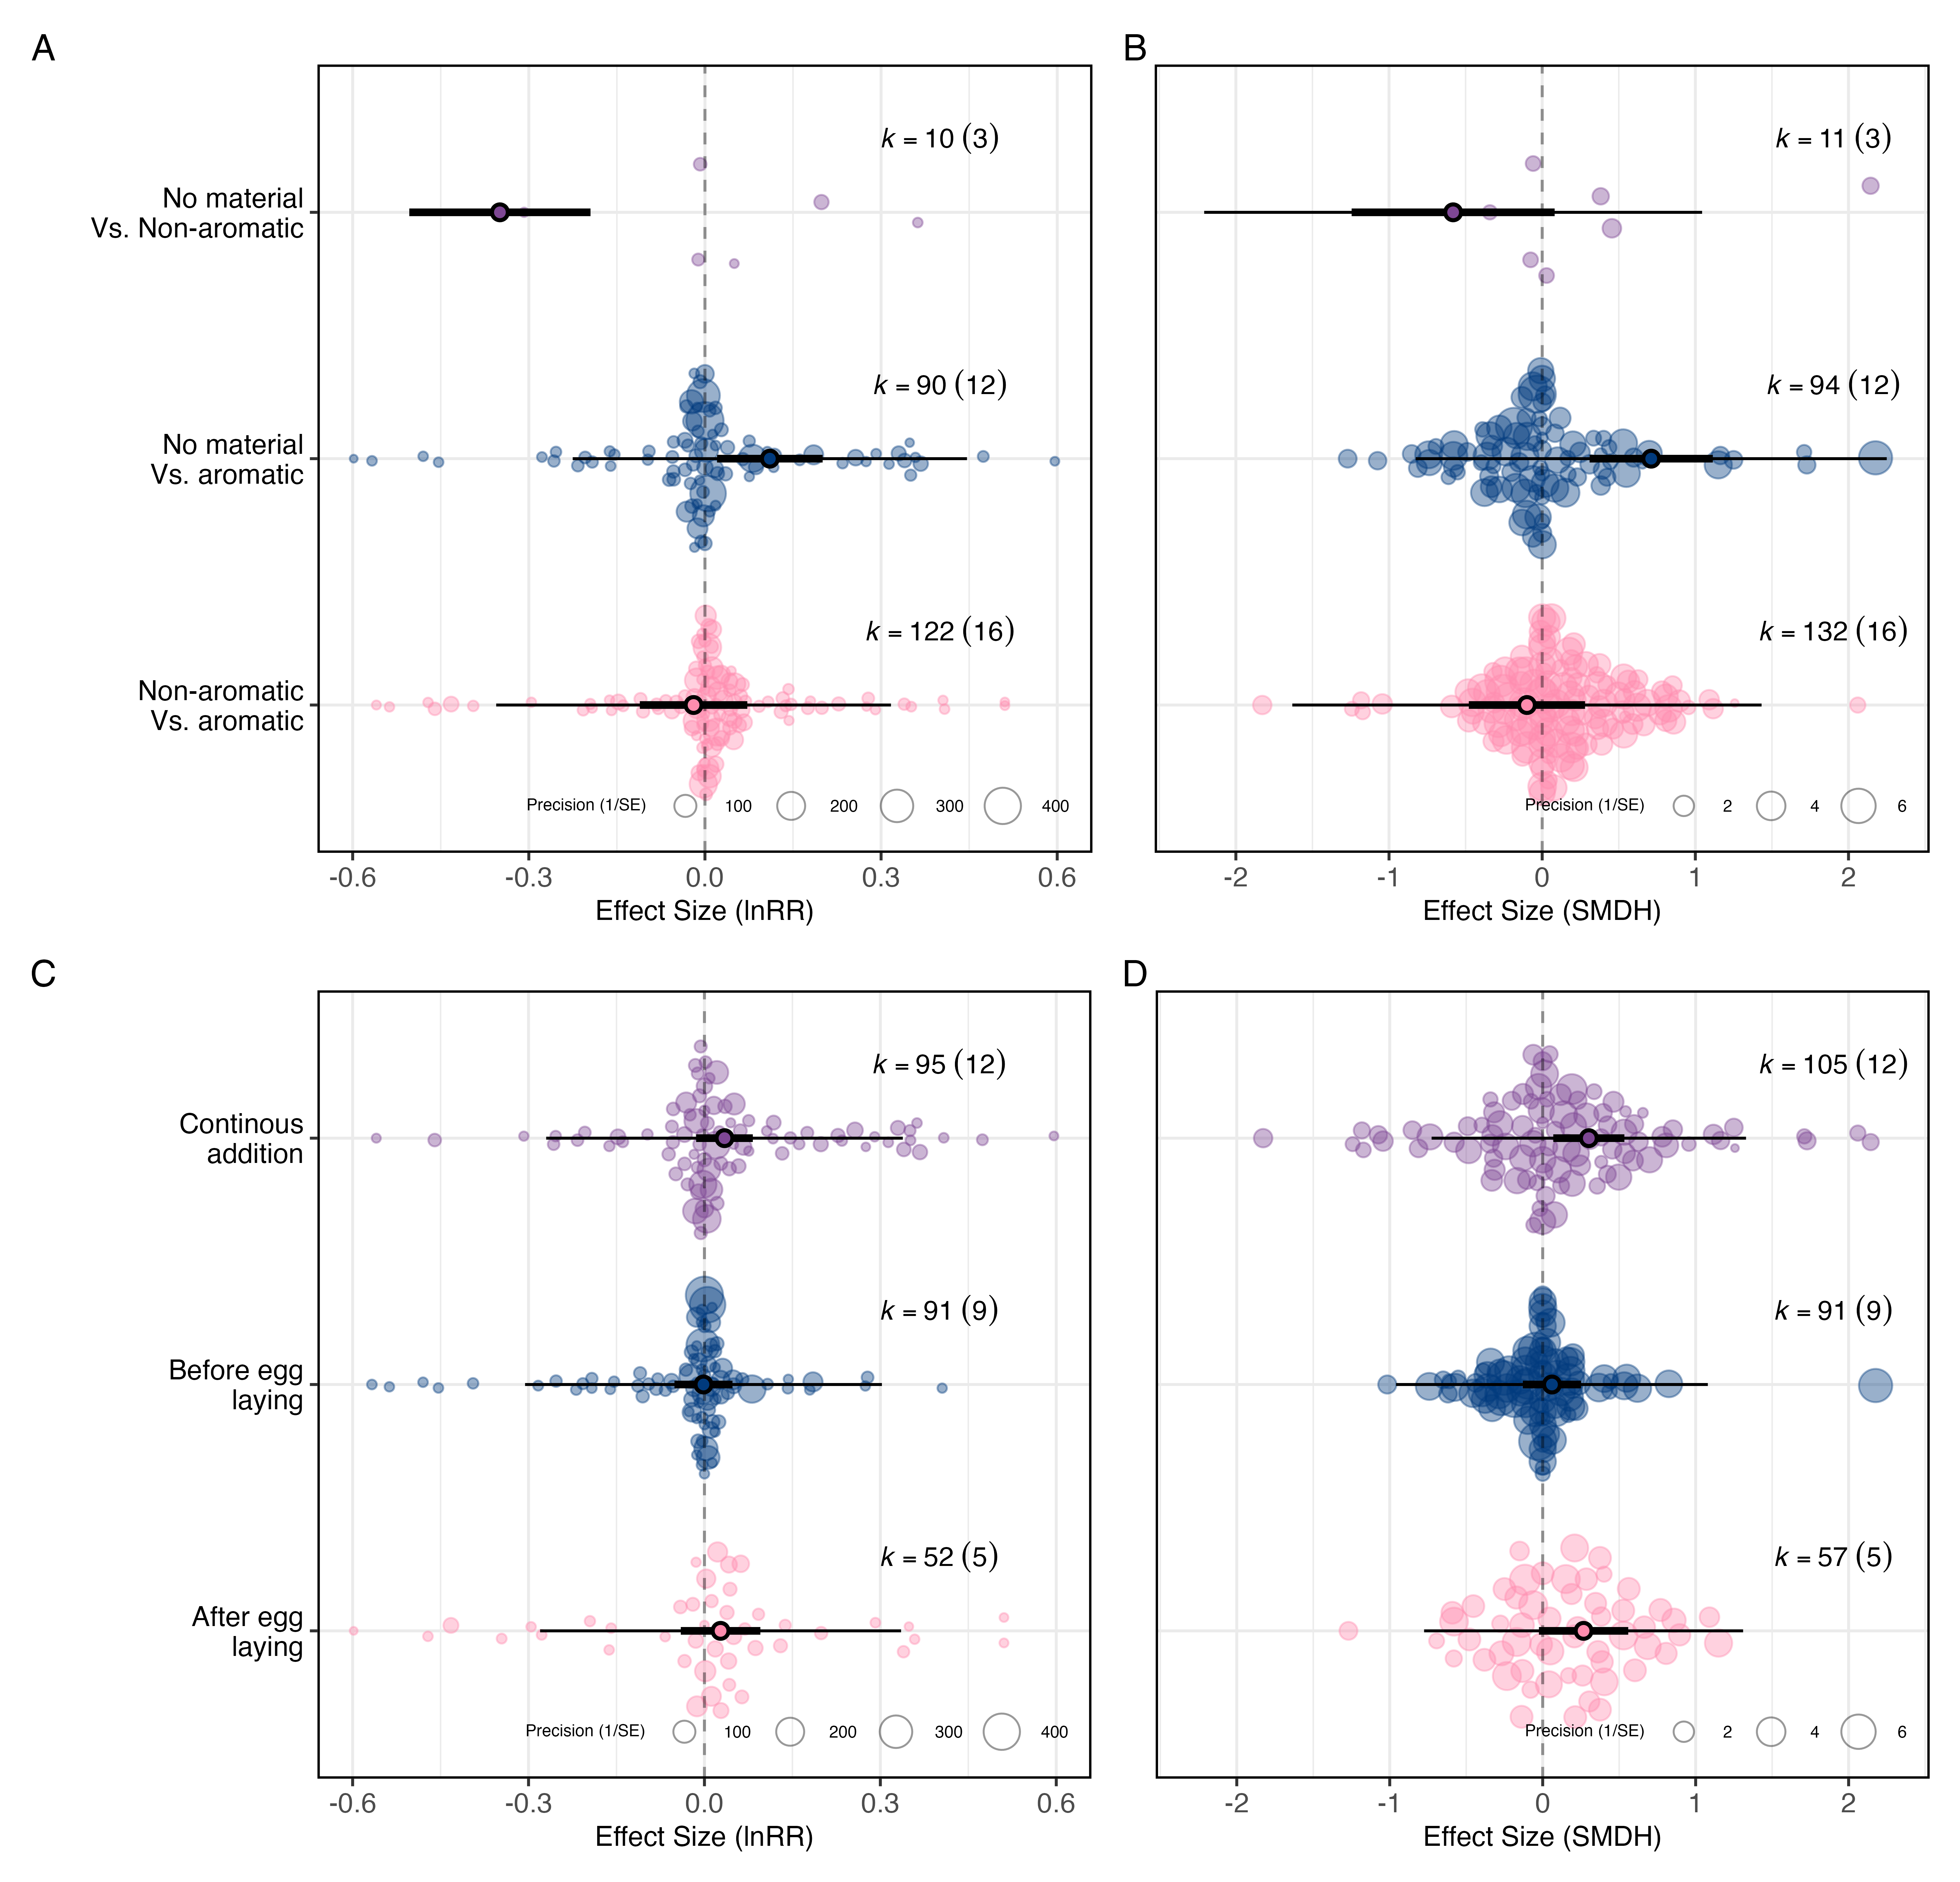
\includegraphics[keepaspectratio]{figures/Figure_design_time_gnm_addition_cropped.png}}

}

\caption{\label{figmain-design-time}Experimental designs comparing nests
with aromatic green nest material against nests without any green
material, and those adding the material continuously, lead to the
largest fitness estimates. Orchard plots of the multilevel
meta-regressions showing the overall effect of green nest material
depending on experimental design for (A: log response ratio (lnRR); B:
standardised mean difference (SMD(H)), and time of green nest material
addition (C: log response ratio (lnRR); D: standardised mean difference
(SMD(H)). Mean estimates (black circles), 95\% confidence intervals
(thicker bars) and prediction intervals (thinner bars) are shown along
the individual data points (transparently coloured circles) scaled by
precision (inverse of standard error). k: number of effect sizes (number
of studies is shown in the brackets). X-axes are truncated for
legibility, which partially explains any apparent asymmetry (complete
figures in Section \quartofigsuppref{figsupp-design-time}).}

\end{figmain}%

Second, the overall positive effect of GNM on fitness outcomes tended to
be larger when GNM was added continuously throughout the nesting phase
(Figure\ref{figmain-design-time}C,D). The overall effect was positive
and statistically significant for SMD(H) when material was continuously
and experimentally added to the nest (lnRR\textsubscript{continously} =
0.034, 95\% CI: {[}-0.014, 0.083{]}, 95\% PI: {[}-0.270, 0.338{]},
p-value = 0.165, k = 95, n = 12; SMD(H)\textsubscript{continously} =
0.302, 95\% CI: {[} 0.069, 0.534{]}, 95\% PI: {[}-0.726, 1.329{]},
p-value = 0.011, k = 105, n = 12), whereas the effect was small and
statistically non-significant when added before egg hatching
Table\ref{tabmain-MLMR}. Last, the overall effect also tended to be
positive for SMD(H) when GNM was added after egg hatching only, although
only marginally so (SMD(H)\textsubscript{after\_egg\_hatching} = 0.267,
95\% CI: {[}-0.024, 0.559{]}, 95\% PI: {[}-0.775, 1.310{]}, p-value =
0.072, k = 57, n = 5; Table\ref{tabmain-MLMR}). The three categories did
not differ statistically significantly from each other
(p-value\textsubscript{lnRR} \textgreater{} 0.307 and
p-value\textsubscript{SMD(H)} \textgreater{} 0.243 in all cases). The
timing of GNM addition explained little heterogeneity
(\(R^2_{marginal(lnRR)}\)= 1.2\% and \(R^2_{marginal(SMD(H))}\)= 4.5\%).

Third, although none of the species-specific mean estimates were
statistically significant, most were positive
\quartofigsuppref{figsupp-MR}, Table\ref{tabmain-MLMR}, and bird species
identity explained a non-negligible amount of heterogeneity
(\(R^2_{marginal(lnRR)}\)= 5.3\% and \(R^2_{marginal(SMDH)}\)= 8.5\%).
Fourth, most fitness proxy-specific mean estimates were positive, but
only morphology was statistically significant, and only for SMD(H)
(SMDH\textsubscript{morphology} = 0.310, 95\% CI: {[} 0.112, 0.509{]},
95\% PI: {[}-0.723, 1.343{]}, p-value = 0.002, k = 65, n = 15;
\quartofigsuppref{figsupp-MR}; Table\ref{tabmain-MLMR}) and fitness
proxy category accounted for a small amount of heterogeneity
(\(R^2_{marginal(lnRR)}\)= 3.7\% and \(R^2_{marginal(SMD(H))}\)= 2.4\%).
Fifth, for the subset of outcomes relating to pathogen and parasitic
load, estimates for arthropods and micro-organisms did not differ
statistically significantly (\quartofigsuppref{figsupp-MR} ;
Table\ref{tabmain-MLMR}) and the type of parasite or pathogen explained
little heterogeneity (\(R^2_{marginal(lnRR)}\)= 0.4\% and
\(R^2_{marginal(SMD(H))}\)= 1.6\%). Lastly, the evaluation of potential
risk-of-bias categories (i.e., blinding, random assignment to each
treatment, and partial reporting) were limited by the small number of
studies in some categories (details in
\quartotabsuppref{tabsupp-SA-RoB})

\begin{tabmain}

\centering{

\pandocbounded{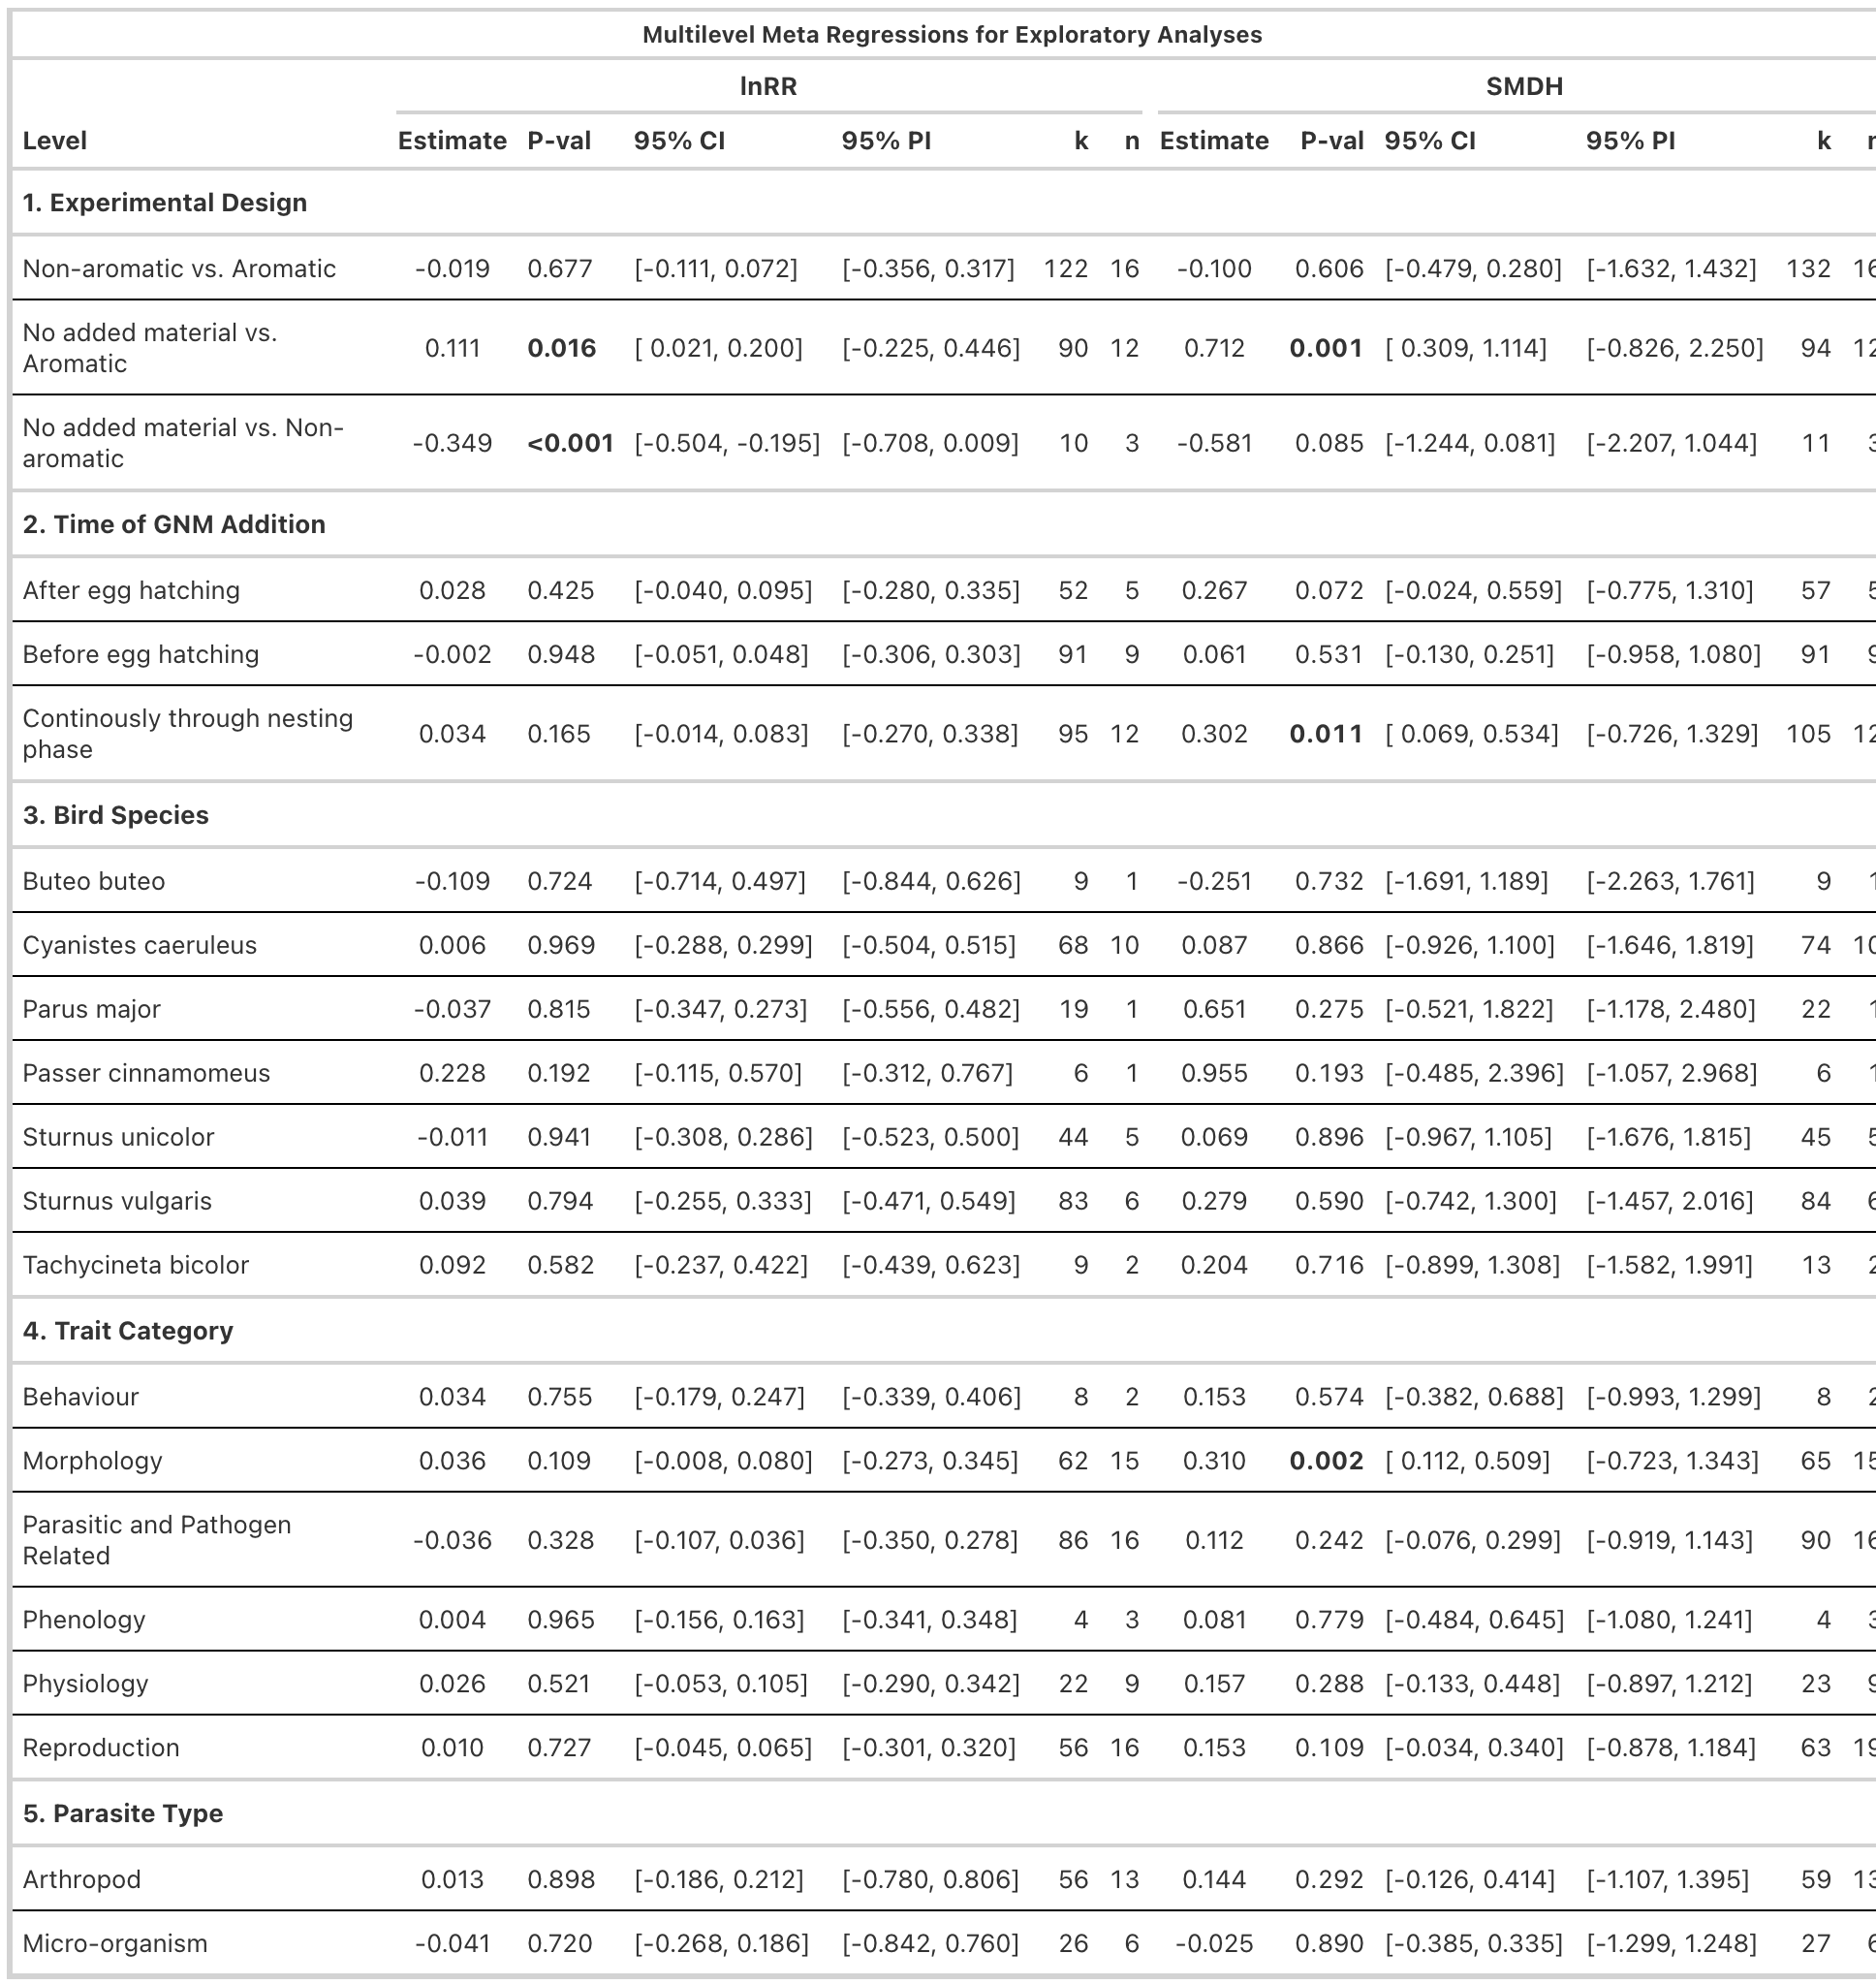
\includegraphics[keepaspectratio]{tables/MLMR_table.png}}

}

\caption{\label{tabmain-MLMR}Results from multilevel meta-regressions
testing how experimental design, timing of green nest material (GNM)
addition, bird species, trait category, and parasite type influence the
effect of GNM on fitness outcomes. Columns show model estimates,
p-values, 95\% confidence intervals (CI), 95\% prediction intervals
(PI), number of effect sizes (k), and number of studies (n) for both
effect size metrics: log response ratio (lnRR) and standardized mean
difference (SMD(H)). Statistically significant results (p \textless{}
0.05) are shown in bold.}

\end{tabmain}%

\subsection{Publication Bias}\label{publication-bias}

\textsubscript{Source:
\href{https://shreyadimri.github.io/Green_Nest_Material/manuscript_GNM.qmd.html}{Article
Notebook}}

We found no conclusive evidence for publication bias in the published
literature \quartofigsuppref{figsupp-pub-bias}. There was no statistical
evidence for small-study effect for lnRR (lnRR\textsubscript{intercept}=
0.003, 95\% CI: {[}-0.066, 0.072{]}, p-value = 0.926,
lnRR\textsubscript{slope} = 0.079, 95\% CI: {[}-0.215; 0.373{]}, p-value
= 0.595, k = 221, n = 24, \(R^2_{marginal(lnRR)}\)= 0.3\%). For SMD(H),
there was a tendency for effect sizes to be larger when sample size was
smaller but this relationship was marginally statistically significant
(SMDH\textsubscript{slope} = 1.393, 95\% CI: {[}-0.143, 2.929{]},
p-value = 0.075, k = 235, n = 24, \(R^2_{marginal(SMD(H))}\)= 8.3\%)
with the overall adjusted effect decreasing substantially
(SMDH\textsubscript{intercept} = -0.035, 95\% CI: {[}-0.319, 0.249{]},
p-value = 0.809). In addition, since published effect sizes did not seem
to change considerably over time, our analyses suggest no clear evidence
of decline effects in published effect sizes (see
\quartofigsuppref{figsupp-pub-bias}).

\section{Discussion}\label{discussion}

Our pre-registered systematic review and meta-analysis provide the first
quantitative synthesis of the adaptive function of green nest material
(GNM) in birds. By aggregating all relevant experimental evidence on
different fitness proxies, we found that, on average, GNM has a small
positive effect on fitness. Our results were generally consistent across
two effect size metrics and robust to various sensitivity analyses;
however, the moderate-to-high levels of heterogeneity among effect sizes
indicate context-dependency. By testing several biological and
methodological moderators, we found that experimental design explains
the highest proportion of heterogeneity, raising the question of whether
it is the plants' aromatic volatile compounds alone that explain the
observed association between GNM and fitness. Below, we discuss our
findings in specific contexts, highlight knowledge gaps and potential
biases in the current literature, and suggest directions for future
research.

Although our synthesis shows that the addition of GNM is associated with
an increase in fitness estimates, we found no clear support for either
of the two functional hypotheses traditionally proposed: the courtship
hypothesis and parental care hypothesis (i.e., nest protection and drug
hypotheses combined). Despite several studies explicitly looking into
the courtship hypothesis (e.g., \citep{lopez-rull2009};
\citep{tomás2013}), only a few fitness proxies could be exclusively
linked to this mechanism (e.g., courtship time, male provisioning), and
these showed no effect of GNM. Similarly, fitness proxies exclusively
associated with the parental care hypothesis, such as parasite loads and
nestling health, also showed no effect of GNM. The latter finding is
particularly surprising because the parental care hypothesis, which is
nest protection and drug hypothesis combined, has been most frequently
tested. While studies testing the courtship hypothesis have suggested
that the aromatic volatile compounds could help receivers of the signal
(often females) detect the presence of GNM in dark cavity nests, it is
the parental care hypothesis that has stressed the importance of these
compounds, perhaps explaining their widespread consideration. Our
findings, however, challenge this assumption since experimental designs
comparing aromatic vs.~non-aromatic GNM, which correspond to over half
of all tests, do not suggest a fitness effect, whereas those comparing
aromatic vs.~no material do. Surprisingly, though, comparing
non-aromatic vs.~no material suggested a negative effect of non-aromatic
GNM on fitness; though this result should be interpreted cautiously, as
it was based on only three studies (k = 10 effect sizes). Importantly,
experimental design alone explained about one-fourth of the observed
heterogeneity (\(R^2_{marginal}\) 24-28\%). In addition, only proxies
that could not be clearly assigned to either of the functional
hypotheses (e.g., survival rate, nestling morphology), which~ were then
categorized as being associated with ``both'' hypotheses, showed a clear
positive effect. This ambiguity reflects the challenge of interpreting
many fitness proxies in relation to an underlying function, as they are
likely influenced by multiple overlapping processes. Our results call
for reconsidering the importance of aromatic volatile compounds, and
thus, the mechanisms involved in the adaptive function of GNM.

The overall effect of GNM was heterogeneous and mainly associated with
within-study variation, with little to none among-study variation. This
suggests that, once methodological and biological factors within studies
are accounted for, the overall effect found would be potentially
generalisable across studies. In addition to experimental design (see
paragraph above), another methodological moderator that we tested was
the time of GNM addition (\(R^2_{ma rginal}\)= 1-5\%). Continuous
addition of GNM throughout the nesting period showed greater positive
effects than addition restricted to before or after egg hatching.
Previous work on blue tits has shown that the concentration of active
compounds released by the aromatic plants can decrease within 24 hours
\citep{petit2002}, and females often replace experimentally removed
herbs \citep{mennerat2008, banbura1995}. TThis repeated addition may
help maintain an environment high in volatiles that are hostile to
parasites. However, the presence of fresh GNM could also lead to a
positive effect on fitness via structural or micro-climate benefits.
Fresh GNM can act as a renewable lining that improves nest insulation
and humidity buffering as nest material gradually desiccates
\citep{mertens1977, taverner1933}. Such micro-climate stability can
accelerate nestling development while reducing thermoregulatory costs
for the parents \citep{mainwaring2013}. In addition, regular
replenishment of GNM by birds could also help replace the wilted
material in the nest, thus maintaining nest structure and helping dilute
faecal matter or food debris in the nest (i.e., hygiene function;
\citep{peralta-sanchez2010}).

Among the biological moderators tested, species identity seemed the most
important one (\(R^2_{marginal}\) = 5-9\%), providing some evidence for
species-specific effects; however, note that three species were
represented in only one study each. Such variation across species is not
unexpected, since some (e.g., Tachycineta bicolor) do not add GNM in
nature, while the others species do. Additionally, species-specific
differences in life-history traits, nest construction, or habitat
condition, and their interplay likely influence how GNM affects fitness.
The second most important biological moderator was the fitness proxy
category (\(R^2_{marginal}\) = 2-4\%), potentially indicating
differences in validity across fitness proxies or reflecting differences
among underlying mechanisms. Among all categories, morphological
outcomes (e.g., nestling mass, tarsus length, wing length) showed the
largest positive effects, suggesting that GNM has a more pronounced
effect on offspring development or growth. Morphology was the second
most commonly measured fitness proxy across studies, likely because it
is relatively easy to measure and less prone to measurement error.
However, while widely used as an indicator of offspring condition, these
morphological measures remain indirect fitness proxies. All other
fitness proxy categories, including physiology, reproduction, phenology,
and behaviour, showed small to moderate positive effects, whereas
proxies related to parasite or pathogen load, despite being the most
commonly investigated, showed weak and inconsistent effects. Parasite
reduction is central to one of the two mechanisms within the parental
care hypothesis (the nest protection hypothesis, \citep{wimberger1984};
\citep{clark1985}). Our results further emphasise that despite its
prominence, there is a lack of clear overall evidence for the parental
care hypothesis. The other hypothesis categorised within the parental
care hypothesis (i.e., the drug hypothesis; \citep{gwinner2000} ;
\citep{mennerat2009a}), proposes an increase in offspring survival, with
volatile compounds directly enhancing offspring immune function and/or
health independent of parasite or pathogen control. While the largest
positive effects of morphology could support the drug hypothesis, it
should be noted that (i) the mechanism linking volatiles to enhanced
offspring immune function or health is unclear, (ii) our results suggest
that non-aromatic GNM may play a role, and (iii) several other
mechanisms could also be at play. For example, improved offspring
morphological condition could result from enhanced micro-climate of the
nest (e.g., \citep{corregidor-castro2021}), better incubation of the
eggs or indirectly through sexually selected male traits, as suggested
by the courtship hypothesis.

When interpreting our results, it is important to acknowledge some
constraints of the study and in the available evidence. The overall
effect of GNM differed between the two effect size metrics, which make
distinct assumptions regarding the underlying biological processes and
the statistical properties. These divergent results highlight the
importance of choosing appropriate effect size metrics for a
meta-analysis that align with the biological data at hand or in cases
where several different types of measures are present, using both
\citep{yang2024}. We found high reporting quality in the primary study
included in our meta-analysis, with only 0.06\% partial reporting, but
some evidence of small-study effects. After adjusting for this, the
effect of GNM was no longer significant. To reduce the influence of
small-study effects we contacted all authors for unpublished data, but
could only find access to two studies. In addition, many studies had
very low sample sizes (41\% of the effect sizes were based on fewer than
10 nests per group), which reduces power and increases heterogeneity.
Furthermore, studies remain heavily biased towards just three bird
species, limiting our ability to infer broad patterns of this behaviour.
Expanding the scope to other bird species with diverse nesting ecologies
and habitat conditions can be useful in understanding the adaptive
benefits of this behaviour.

\section{Conclusion}\label{conclusion}

After more than 40 years of research on this topic, ours is the first
quantitative synthesis confirming an overall effect of green nest
material on fitness in birds. Despite the moderate-to-high heterogeneity
observed, our results suggest that the effect may be generalisable
across studies once methodological and biological factors within studies
are accounted for. An important caveat, however, is that our small-study
effects analysis, although non-conclusively, indicates that accounting
for potentially missing studies could cause the observed effect to
disappear, despite our efforts to include unpublished work. Moreover,
our study clearly emphasises that the functions remain largely unclear
and challenges the assumption that volatile compounds alone explain the
relationship between green nest material and fitness. Future studies
should consider focusing on experimental designs that disentangle the
different functional hypotheses suggested, prioritising fitness proxies
that are more directly linked to fitness, as well as to test explicitly,
rather than assume, the role of volatiles. In addition, theoretical work
could further solidify the field's foundations and yield testable
predictions. Altogether, our synthesis contributes to a more nuanced
understanding of the adaptive significance of one of the most
fascinating and most studied natural structures: bird nests, as well as
opens the door to several questions still unanswered.

\subsection{Data and Code Availability
Statement}\label{data-and-code-availability-statement}

All data and code associated with this project can be found on GitHub at
{[}\url{https://github.com/shreyadimri/Green_Nest_Material}{]}. It is
also available on Zenodo {[}\textbf{insert link later}{]}.

\subsection{Author contributions}\label{author-contributions}

\textbf{SD:} Conceptualisation, Data curation, Formal analysis,
Investigation (lead), Methodology, Project administration, Software,
Validation, Visualization, Writing - original draft (lead), review \&
editing; \textbf{TR:} Conceptualisation, Investigation (equal), Writing
- review \& editing; \textbf{JMGS:} Conceptualisation, Investigation
(equal), Writing - review \& editing; \textbf{MO:} Investigation
(supporting), Validation; \textbf{AST:} Conceptualisation, Funding
acquisition, Methodology, Supervision, Writing - original draft
(supporting), review \& editing

\subsection{Conflict of interest}\label{conflict-of-interest}

Authors declare no competing interests.

\subsection{Acknowledgements}\label{acknowledgements}

We thank Klaus Reinhold for his support. We also thank all the authors
who replied to our emails and who addressed our questions. We are
particularly grateful to those who kindly shared their data: Adele
Mennerat, Dave Shutler and Gustavo Tomás Gutiérrez.

\subsection{Funding}\label{funding}

SD and AST were funded by the DFG (Deutsche Forschungsgemeinschaft) as
part of the SFB TRR 212 (NC³) Second Phase 2022-2025 (Project number
316099922), and MO by the First Phase 2018-2021 (Project number
396780709). JMGS was financially supported by a Walter Benjamin
Fellowship from the DFG. TR was financially supported by a Research
Grant for Doctoral Programmes by the DAAD (Deutscher Akademischer
Austauschdienst).

\section{References}\label{references}

\renewcommand{\bibsection}{}
\bibliography{references.bib}

\section{Supplementary Appendix}\label{supplementary-appendix}

\subsection{PRISMA Checklist}\label{prisma-checklist}

\begin{tabsupp}

\centering{

Completed PRISMA-EcoEvo Checklist \citep{odea2021}: This checklist shows
how the systematic review and meta-analysis on green nest material and
fitness outcomes complies with reporting standards in ecology and
evolutionary biology

}

\caption{\label{tabsupp-checklist}}

\end{tabsupp}%

\begin{longtable}[]{@{}
  >{\raggedright\arraybackslash}p{(\linewidth - 10\tabcolsep) * \real{0.1500}}
  >{\raggedright\arraybackslash}p{(\linewidth - 10\tabcolsep) * \real{0.1000}}
  >{\raggedright\arraybackslash}p{(\linewidth - 10\tabcolsep) * \real{0.1000}}
  >{\raggedright\arraybackslash}p{(\linewidth - 10\tabcolsep) * \real{0.2000}}
  >{\raggedright\arraybackslash}p{(\linewidth - 10\tabcolsep) * \real{0.1500}}
  >{\raggedright\arraybackslash}p{(\linewidth - 10\tabcolsep) * \real{0.3000}}@{}}
\toprule\noalign{}
\endhead
\bottomrule\noalign{}
\endlastfoot
\textbf{Checklist item} & \textbf{Item score} & \textbf{Sub-item number}
& \textbf{Sub-item} & \textbf{Reported by authors?} & \textbf{Notes} \\
\textbf{Title and abstract} & \textbf{100\%} & 1.1 & Identify the review
as a systematic review, meta-analysis, or both & Yes & Identified in
title and in abstract as both a systematic review and a meta-analysis \\
& & 1.2 & Summarise the aims and scope of the review & Yes & In the
abstract \\
& & 1.3 & Describe the data set & Yes & In the abstract \\
& & 1.4 & State the results of the primary outcome & Yes & In the
abstract \\
& & 1.5 & State conclusions & Yes & In the abstract \\
& & 1.6 & State limitations & Yes & In the abstract \\
\textbf{Aims and questions} & \textbf{100\%} & 2.1 & Provide a rationale
for the review & Yes & Rationale explained in the Introduction in
detail \\
& & 2.2 & Reference any previous reviews or meta-analyses on the topic &
Yes & Clearly stated twice in the introduction \\
& & 2.3 & State the aims and scope of the review (including its
generality) & Yes & Scope (only birds and experimental studies)
explained along with the aims in the last paragraph of Introduction \\
& & 2.4 & State the primary questions the review addresses (e.g.~which
moderators were tested) & Yes & Moderators tested are clearly stated in
the methods in the data analysis section. \\
& & 2.5 & Describe whether effect sizes were derived from experimental
and/or observational comparisons & Yes & Only experimental studies were
selected, described in the last paragraph of introduction as well as the
methods \\
\textbf{Review registration} & \textbf{100\%} & 3.1 & Register review
aims, hypotheses (if applicable), and methods in a time-stamped and
publicly accessible archive and provide a link to the registration in
the methods section of the manuscript. Ideally registration occurs
before the search, but it can be done at any stage before data analysis.
& Yes & \url{https://doi.org/10.17605/OSF.IO/S7J6Z} \\
& & 3.2 & Describe deviations from the registered aims and methods & Yes
& Described in methods wherever applicable \\
& & 3.3 & Justify deviations from the registered aims and methods & Yes
& When applicable, described in the methods \\
\textbf{Eligibility criteria} & \textbf{100\%} & 4.1 & Report the
specific criteria used for including or excluding studies when screening
titles and/or abstracts, and full texts, according to the aims of the
systematic review (e.g.~study design, taxa, data availability) & Yes &
Described briefly in the methods, but mainly in the decision tree (see
Supplementary Materials) \\
& & 4.2 & Justify criteria, if necessary (i.e.~not obvious from aims and
scope. & Yes & Described along with the decision tree (see Supplementary
Materials) \\
\textbf{Finding studies} & \textbf{100\%} & 5.1 & Define the type of
search (e.g.~comprehensive search, representative sample) & Yes &
Comprehensive search conducted, described in methods along with search
string (complete search string provided in the supplementary
materials) \\
& & 5.2 & State what sources of information were sought (e.g.~published
and unpublished studies, personal communications) & Yes & Published,
unpublished as well as personal communications. Described in detail in
the Eligibility Criteria and Data Extraction section of Methods
Section \\
& & 5.3 & Include, for each database searched, the exact search strings
used, with keyword combinations and Boolean operators & Yes & See
complete search string in the Supplementary Materials \\
& & 5.4 & Provide enough information to repeat the equivalent search (if
possible), including the timespan covered (start and end dates) & Yes &
See complete search string details in the Supplementary Materials.
Search dates are described in the methods. \\
\textbf{Study selection} & \textbf{100\%} & 6.1 & Describe how studies
were selected for inclusion at each stage of the screening process
(e.g.~use of decision trees, screening software) & Yes & Abstract-Title
screening was conducted using the R package revtools GUI and Fulltext
screening was conducted in excel manually downloading the articles.
Described in detail in the pre-registration and methods section. The
decision tree is provided in the supplementary materials. \\
& & 6.2 & Report the number of people involved and how they contributed
(e.g.~independent parallel screening) & Yes & Described in detail in the
methods section. All screening decision files are shared as .xls/.csv
files with notes on the decisions made. \\
\textbf{Data collection process} & \textbf{100\%} & 7.1 & Describe where
in the reports data were collected from (e.g.~text or figures) & Yes &
In all files after the data extraction (shared along with the project),
the column data\_location contains this information \\
& & 7.2 & Describe how data were collected (e.g.~software used to
digitize figures, external data sources) & Yes & Described in detail in
the Data extraction section. \\
& & 7.3 & Describe moderator variables that were constructed from
collected data (e.g.~number of generations calculated from years and
average generation time) & Yes & All moderators are described in detail
in the metadata file of the overall dataset. Please see
data\_cleaning.Rmd and data\_preparation.Rmd files for any cleaning done
to the files. All codes are provided along with the dataset. \\
& & 7.4 & Report how missing or ambiguous information was dealt with
during data collection (e.g.~authors of original studies were contacted
for missing descriptive statistics, and/or effect sizes were calculated
from test statistics) & Yes & Described in detail in the data extraction
and effect size calculation section in the methods. \\
& & 7.5 & Report who collected data & Yes & The extractor\_ID column in
the data file has information on the ID of who collected the data. The
methods section also describes the ID of the data collector. \\
& & 7.6 & State the number of extractions that were checked for accuracy
by co-authors & & Described in the methods section along with \% of
disagreement and process of resolution. The data\_checker\_ID column in
the data files has information on the ID of who checked the data. \\
\textbf{Data items} & \textbf{100\%} & 8.1 & Describe the key data
sought from each study & Yes & The priority order of data extraction is
described in detail in the Data extraction section of the methods. \\
& & 8.2 & Describe items that do not appear in the main results, or
which could not be extracted due to insufficient information & Yes & All
information that is excluded from analysis is described in detail in the
methods. Some proxies that could not be included in the analysis for
various reasons are reported in the supplementary material along with
the reason. \\
& & 8.3 & Describe main assumptions or simplifications that were made
(e.g.~categorising both `length' and `mass' as `morphology') & Yes & All
major decisions are described in the methods section, for any remaining
description please check the notes column in the data files. \\
& & 8.4 & Describe the type of replication unit (e.g.~individuals,
broods, study sites) & Yes & Described in the methods, we prioritised
nests as the unit of replication whenever possible. \\
\textbf{Assessment of individual study quality} & \textbf{100\%} & 9.1 &
Describe whether the quality of studies included in the systematic
review or meta-analysis was assessed (e.g.~blinded data collection,
reporting quality, experimental versus observational) & Yes & The risk
of bias assessment performed for the individual studies is described in
the methods and results reported in the results section (See
supplementary material for all model output and figures). The risk of
bias categories we evaluated were blinding, random assignment to each
treatment and partial reporting \\
& & 9.2 & Describe how information about study quality was incorporated
into analyses (e.g.~meta-regression and/or sensitivity analysis) & Yes &
We conducted three meta-regressions using blinding, random assignment to
each treatment and partial reporting as moderators in each analysis. We
reported the outcome briefly in the Results (See supplementary material
for all model output and figures) \\
\textbf{Effect size measures} & \textbf{100\%} & 10.1 & Describe effect
size(s) used & Yes & Described in Effect Size Calculation section in
Methods \\
& & 10.2 & Provide a reference to the equation of each calculated effect
size (e.g.~standardised mean difference, log response ratio) and (if
applicable) its sampling variance & Yes & Described in the Effect Size
Calculation section in Methods. Check data\_preparation.Rmd in Code to
see the exact function, its parameters and any equations that were used
to estimate the effect sizes. \\
& & 10.3 & If no reference exists, derive the equations for each effect
size and state the assumed sampling distribution(s) & Yes & Does not
apply. Any custom equations used from books etc. are clearly mentioned
as well as referenced in the Methods section. \\
\textbf{Missing data} & \textbf{100\%} & 11.1 & Describe any steps taken
to deal with missing data during analysis (e.g.~imputation, complete
case, subset analysis) & Yes & All imputations conducted for the missing
data are stated clearly in the Effect Size Calculations in Methods
Section \\
& & 11.2 & Justify the decisions made to deal with missing data & Yes &
We decided to impute the missing data but also conducted the sensitivity
analysis excluding the imputed value. All justifications are clearly
stated in the methods. \\
\textbf{Meta-analytic model description} & \textbf{100\%} & 12.1 &
Describe the models used for synthesis of effect sizes & Yes & Described
all models in Data Analysis section of the Methods \\
& & 12.2 & The most common approach in ecology and evolution will be a
random-effects model, often with a hierarchical/multilevel structure. If
other types of models are chosen (e.g.~common/fixed effects model,
unweighted model), provide justification for this choice & Yes & Not
applicable, Multilevel meta analytical model and meta-regressions were
conducted. No justification needed \\
\textbf{Software} & \textbf{100\%} & 13.1 & Describe the statistical
platform used for inference (e.g.~R) & Yes & R v4.5.1 was used for the
analysis and is clearly stated in the Methods. \\
& & 13.2 & Describe the packages used to run models & Yes & All packages
and their versions are described in the Methods. \\
& & 13.3 & Describe the functions used to run models & Yes & All
important functions used for running the models are stated in the
Methods. \\
& & 13.4 & Describe any arguments that differed from the default
settings & Yes & We have clearly stated all the important arguments that
differed from the default settings. However, see data\_analysis.Rmd for
full description of the arguments for each model. \\
& & 13.5 & Describe the version numbers of all software used & Yes & All
packages and their versions are described in the Methods. \\
\textbf{Non-independence} & \textbf{100\%} & 14.1 & Describe the types
of non-independence encountered (e.g.~phylogenetic, spatial, multiple
measurements over time) & Yes & See data analysis for more details on
how non-independence was handled. \\
& & 14.2 & Describe how non-independence has been handled & Yes & See
data analysis for more details on how non-independence was handled. \\
& & 14.3 & Justify decisions made & Yes & See data analysis for more
details on how non-independence was handled. \\
\textbf{Meta-regression and model selection} & \textbf{100\%} & 15.1 &
Provide a rationale for the inclusion of moderators (covariates) that
were evaluated in meta-regression models & Yes & All the moderators that
were evaluated were pre-registered with the rationale behind it clearly
stated. See Data analysis for more details (but also see
pre-registration). \\
& & 15.2 & Justify the number of parameters estimated in models, in
relation to the number of effect sizes and studies (e.g.~interaction
terms were not included due to insufficient sample sizes) & Yes & We
described the random effects that were not included in the models in the
Methods section \\
& & 15.3 & Describe any process of model selection & Yes & No model
selection was conducted \\
\textbf{Publication bias and sensitivity analysis} & \textbf{100\%} &
16.1 & Describe assessments of the risk of bias due to missing results
(e.g.~publication, time-lag, and taxonomic biases) & Yes & Time-lag bias
and small study bias are reported in the methods, results and
discussion. \\
& & 16.2 & Describe any steps taken to investigate the effects of such
biases (if present) & Yes & We discussed the effects of potential biases
and conducted a sensitivity analysis accounting these effects for the
two main models. \\
& & 16.3 & Describe any other analyses of robustness of the results,
e.g.~due to effect size choice, weighting or analytical model
assumptions, inclusion or exclusion of subsets of the data, or the
inclusion of alternative moderator variables in meta-regressions & Yes &
All sensitivity analysis are mentioned in the methods, results and
discussed where aproporiate. All the results from the sensitivity
analysis/robustness checks are reported as a table in the supplementary
material. \\
Clarification of post hoc analyses & 100\% & 17.1 & When hypotheses were
formulated after data analysis, this should be acknowledged. & Yes & All
analysis are pre-registered and exploratory analysis are clearly stated
under exploratory analysis both in the pre-registration and final
article \\
Metadata, data, and code & 100\% & 18.1 & Share metadata (i.e.~data
descriptions) & Yes & See data and code availability statement for
details. \\
& & 18.2 & Share data required to reproduce the results presented in the
manuscript & Yes & See data and code availability statement for
details. \\
& & 18.4 & Share analysis scripts (or, if a software package with
graphical user interface (GUI) was used, then describe full model
specification and fully specify choices) & Yes & See data and code
availability statement for details. \\
Results of study selection process & 100\% & 19.1 & Report the number of
studies screened & Yes & Details in method and the PRISMA Flowchart in
supplementary material \\
& & 19.2 & Report the number of studies excluded at each stage of
screening & Yes & Details in method and the PRISMA Flowchart in
supplementary material \\
& & 19.3 & Report brief reasons for exclusion from the full text stage &
Yes & Details in the PRISMA Flowchart in supplementary material \\
& & 19.4 & Present a Preferred Reporting Items for Systematic Reviews
and Meta-Analyses (PRISMA)-like flowchart (www.prisma-statement.org). &
Yes & Figure S1 in supplementary materials is a PRISMA Flowchart \\
Sample sizes and study characteristics & 100\% & 20.1 & Report the
number of studies and effect sizes for data included in meta-analyses &
Yes & Details in method and supplementary tables \\
& & 20.2 & Report the number of studies and effect sizes for subsets of
data included in meta-regressions & Yes & Details in method and
supplementary tables \\
& & 20.3 & Provide a summary of key characteristics for reported
outcomes (either in text or figures; e.g.~one quarter of effect sizes
reported for vertebrates and the rest invertebrates) & Yes & All figures
contain effect sizes (k) and unique articles (n) for different moderator
levels. Summary of reported outcomes is also in the first paragraph of
the Results. \\
& & 20.4 & Provide a summary of limitations of included moderators
(e.g.~collinearity and overlap between moderators) & NA & All moderators
tested were categorical and only publication year was a continuous
moderator. Therefore, no collinearity or overlap is possible. \\
& & 20.5 & Provide a summary of characteristics related to individual
study quality (risk of bias) & Yes & This data is presented in dataset
in columns blinding, missing\_data, random\_assignment \\
Meta-analysis & 100\% & 21.1 & Provide a quantitative synthesis of
results across studies, including estimates for the mean effect size,
with confidence/credible intervals & Yes & See results and supplementary
material for detail of all the synthesis. \\
Heterogeneity & 100\% & 22.1 & Report indicators of heterogeneity in the
estimated effect (e.g.~I2, tau2 and other variance components) & Yes &
All estimates of heterogeneity are reported in the results and model
table. Also see supplementary material for the results not reported in
the main text. \\
Meta-regression & 100\% & 23.1 & Provide estimates of meta-regression
slopes (i.e.~regression coefficients) and confidence/credible intervals
& Yes & See results and supplementary material for detail of all the
synthesis. \\
& & 23.2 & Include estimates and confidence/credible intervals for all
moderator variables that were assessed (i.e.~complete reporting) & Yes &
See results and supplementary material for detail of all the
synthesis. \\
& & 23.3 & Report interactions, if they were included & NA & There were
no interactions included \\
& & 23.4 & Describe outcomes from model selection, if done (e.g.~R2 and
AIC) & NA & No model selection was conducted. \\
Outcomes of publication bias and sensitivity analysis & 100\% & 24.1 &
Provide results for the assessments of the risks of bias (e.g.~Egger's
regression, funnel plots) & Yes & Risk of bias was assessed using
meta-regression models with moderator levels for blinding, missing data,
random assignment in experiments and reported in results (and see
supplementary material for complete details). We also reported
meta-regressions for publication bias (time-lag bias and small-study
effects) in results (and see supplementary material for complete
details) \\
& & 24.2 & Provide results for the robustness of the review's results
(e.g.~subgroup analyses, meta-regression of study quality, results from
alternative methods of analysis, and temporal trends) & Yes & All
robustness checks/sensitivity analysis conducted are reported in full
detail in the supplementary material and mentioned in the results
clearly. \\
Discussion & 100\% & 25.1 & Summarise the main findings in terms of the
magnitude of effect & Yes & \\
& & 25.2 & Summarise the main findings in terms of the precision of
effects (e.g.~size of confidence intervals, statistical significance) &
Yes & We use confidence intervals, prediction intervals and statistical
significance to discuss the precision of the effects in the results and
discussion section. \\
& & 25.3 & Summarise the main findings in terms of their heterogeneity &
Yes & We report and discuss the heterogeneity and explore some of the
possible causes of it in our results and discussion. \\
& & 25.4 & Summarise the main findings in terms of their
biological/practical relevance & Yes & We have discussed all important
findings in terms of their biological and practical implications \\
& & 25.5 & Compare results with previous reviews on the topic, if
available & Yes & We have discussed the results comparing them to other
published literature (including two narrative reviews that summarise the
field) but no quantitative review on the field exists to compare the
results with. \\
& & 25.6 & Consider limitations and their influence on the generality of
conclusions, such as gaps in the available evidence (e.g.~taxonomic and
geographical research biases) & Yes & We discuss the limitations of the
evidence. \\
Contributions and funding & 100\% & 26.1 & Provide names, affiliations,
and funding sources of all co-authors & Yes & See section Fundings \\
& & 26.2 & List the contributions of each co-author & Yes & See section
Author Contributions \\
& & 26.3 & Provide contact details for the corresponding author & Yes &
See manuscript Author details: Shreya Dimri -
shreya.dimri@uni-bielefeld.de \\
& & 26.4 & Disclose any conflicts of interest & Yes & See section
Conflict of interest \\
References & 100\% & 27.1 & Provide a reference list of all studies
included in the systematic review or meta-analysis & Yes & See
supplementary material for a list. \\
& & 27.2 & List included studies as referenced sources (e.g.~rather than
listing them in a table or supplement) & Yes & We have included all the
studies in our meta-analysis within the text of the article in
appropriate places. \\
\end{longtable}

\subsection{PRISMA Flowchart}\label{prisma-flowchart}

\begin{figsupp}

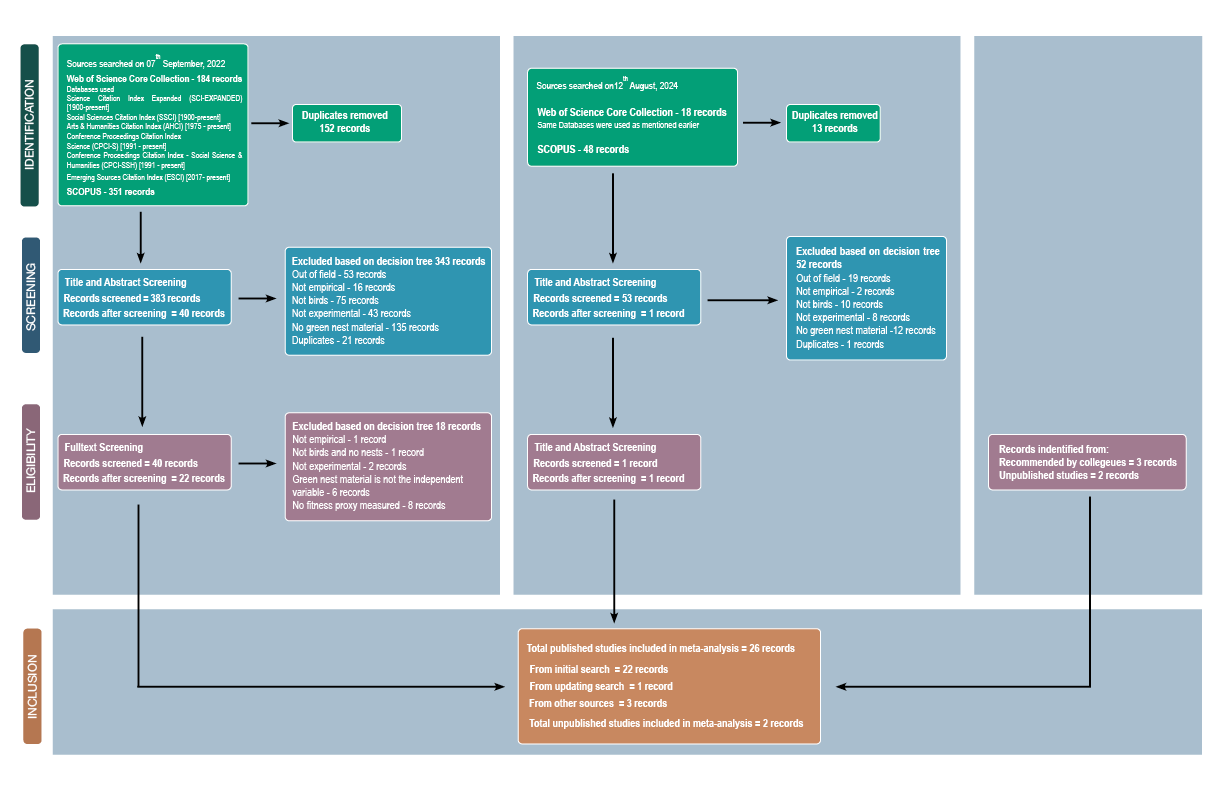
\includegraphics[width=1\linewidth,height=\textheight,keepaspectratio]{figures/Prisma_Flowchart.png}

\caption{\label{figsupp-prisma-flowchart}PRISMA flowchart illustrating
the steps and number of studies included in the systematic review and
meta-analysis on green nest material and fitness outcomes.}

\end{figsupp}%

\subsection{Initial library used for search
validation}\label{initial-library-used-for-search-validation}

\begin{figsupp}

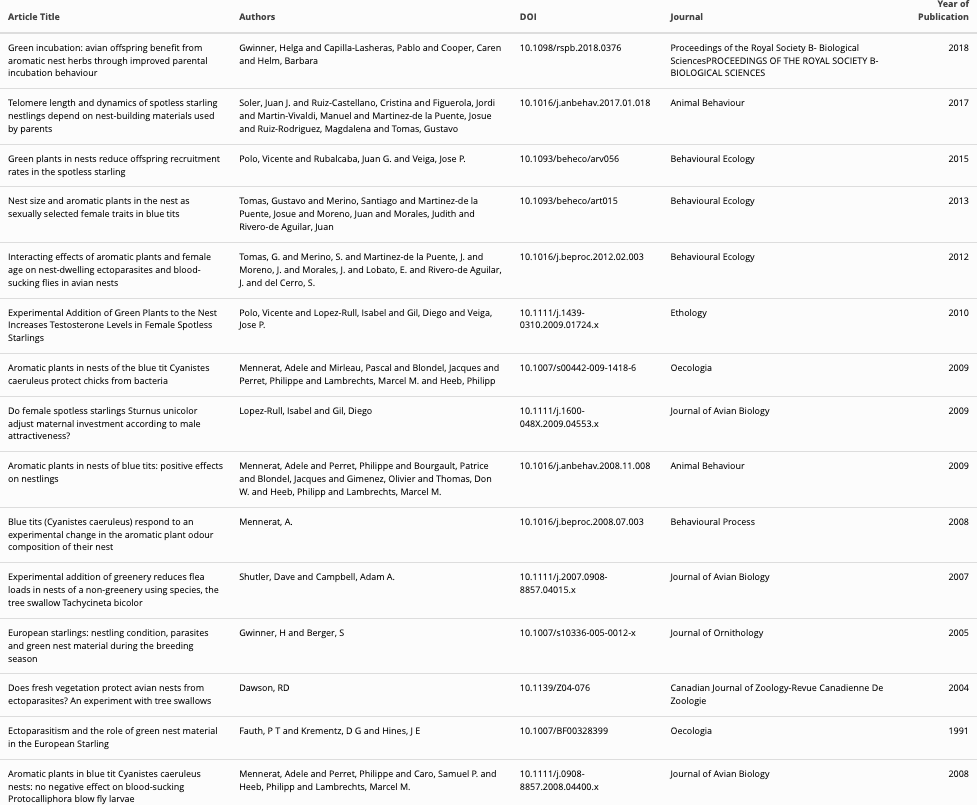
\includegraphics[width=0.9\linewidth,height=\textheight,keepaspectratio]{tables/initial_library.png}

\caption{\label{figsupp-own-library}Validation of the search using our
own initial library of 15 relevant articles: We validated our search
strategy by testing whether it retrieved a pre-compiled set of 15 known
studies on green nest material. Searches conducted successfully
recovered all 15 articles (100\% retrieval), confirming the
effectiveness of our search query}

\end{figsupp}%

\subsection{Decision Tree}\label{decision-tree}

\begin{figsupp}

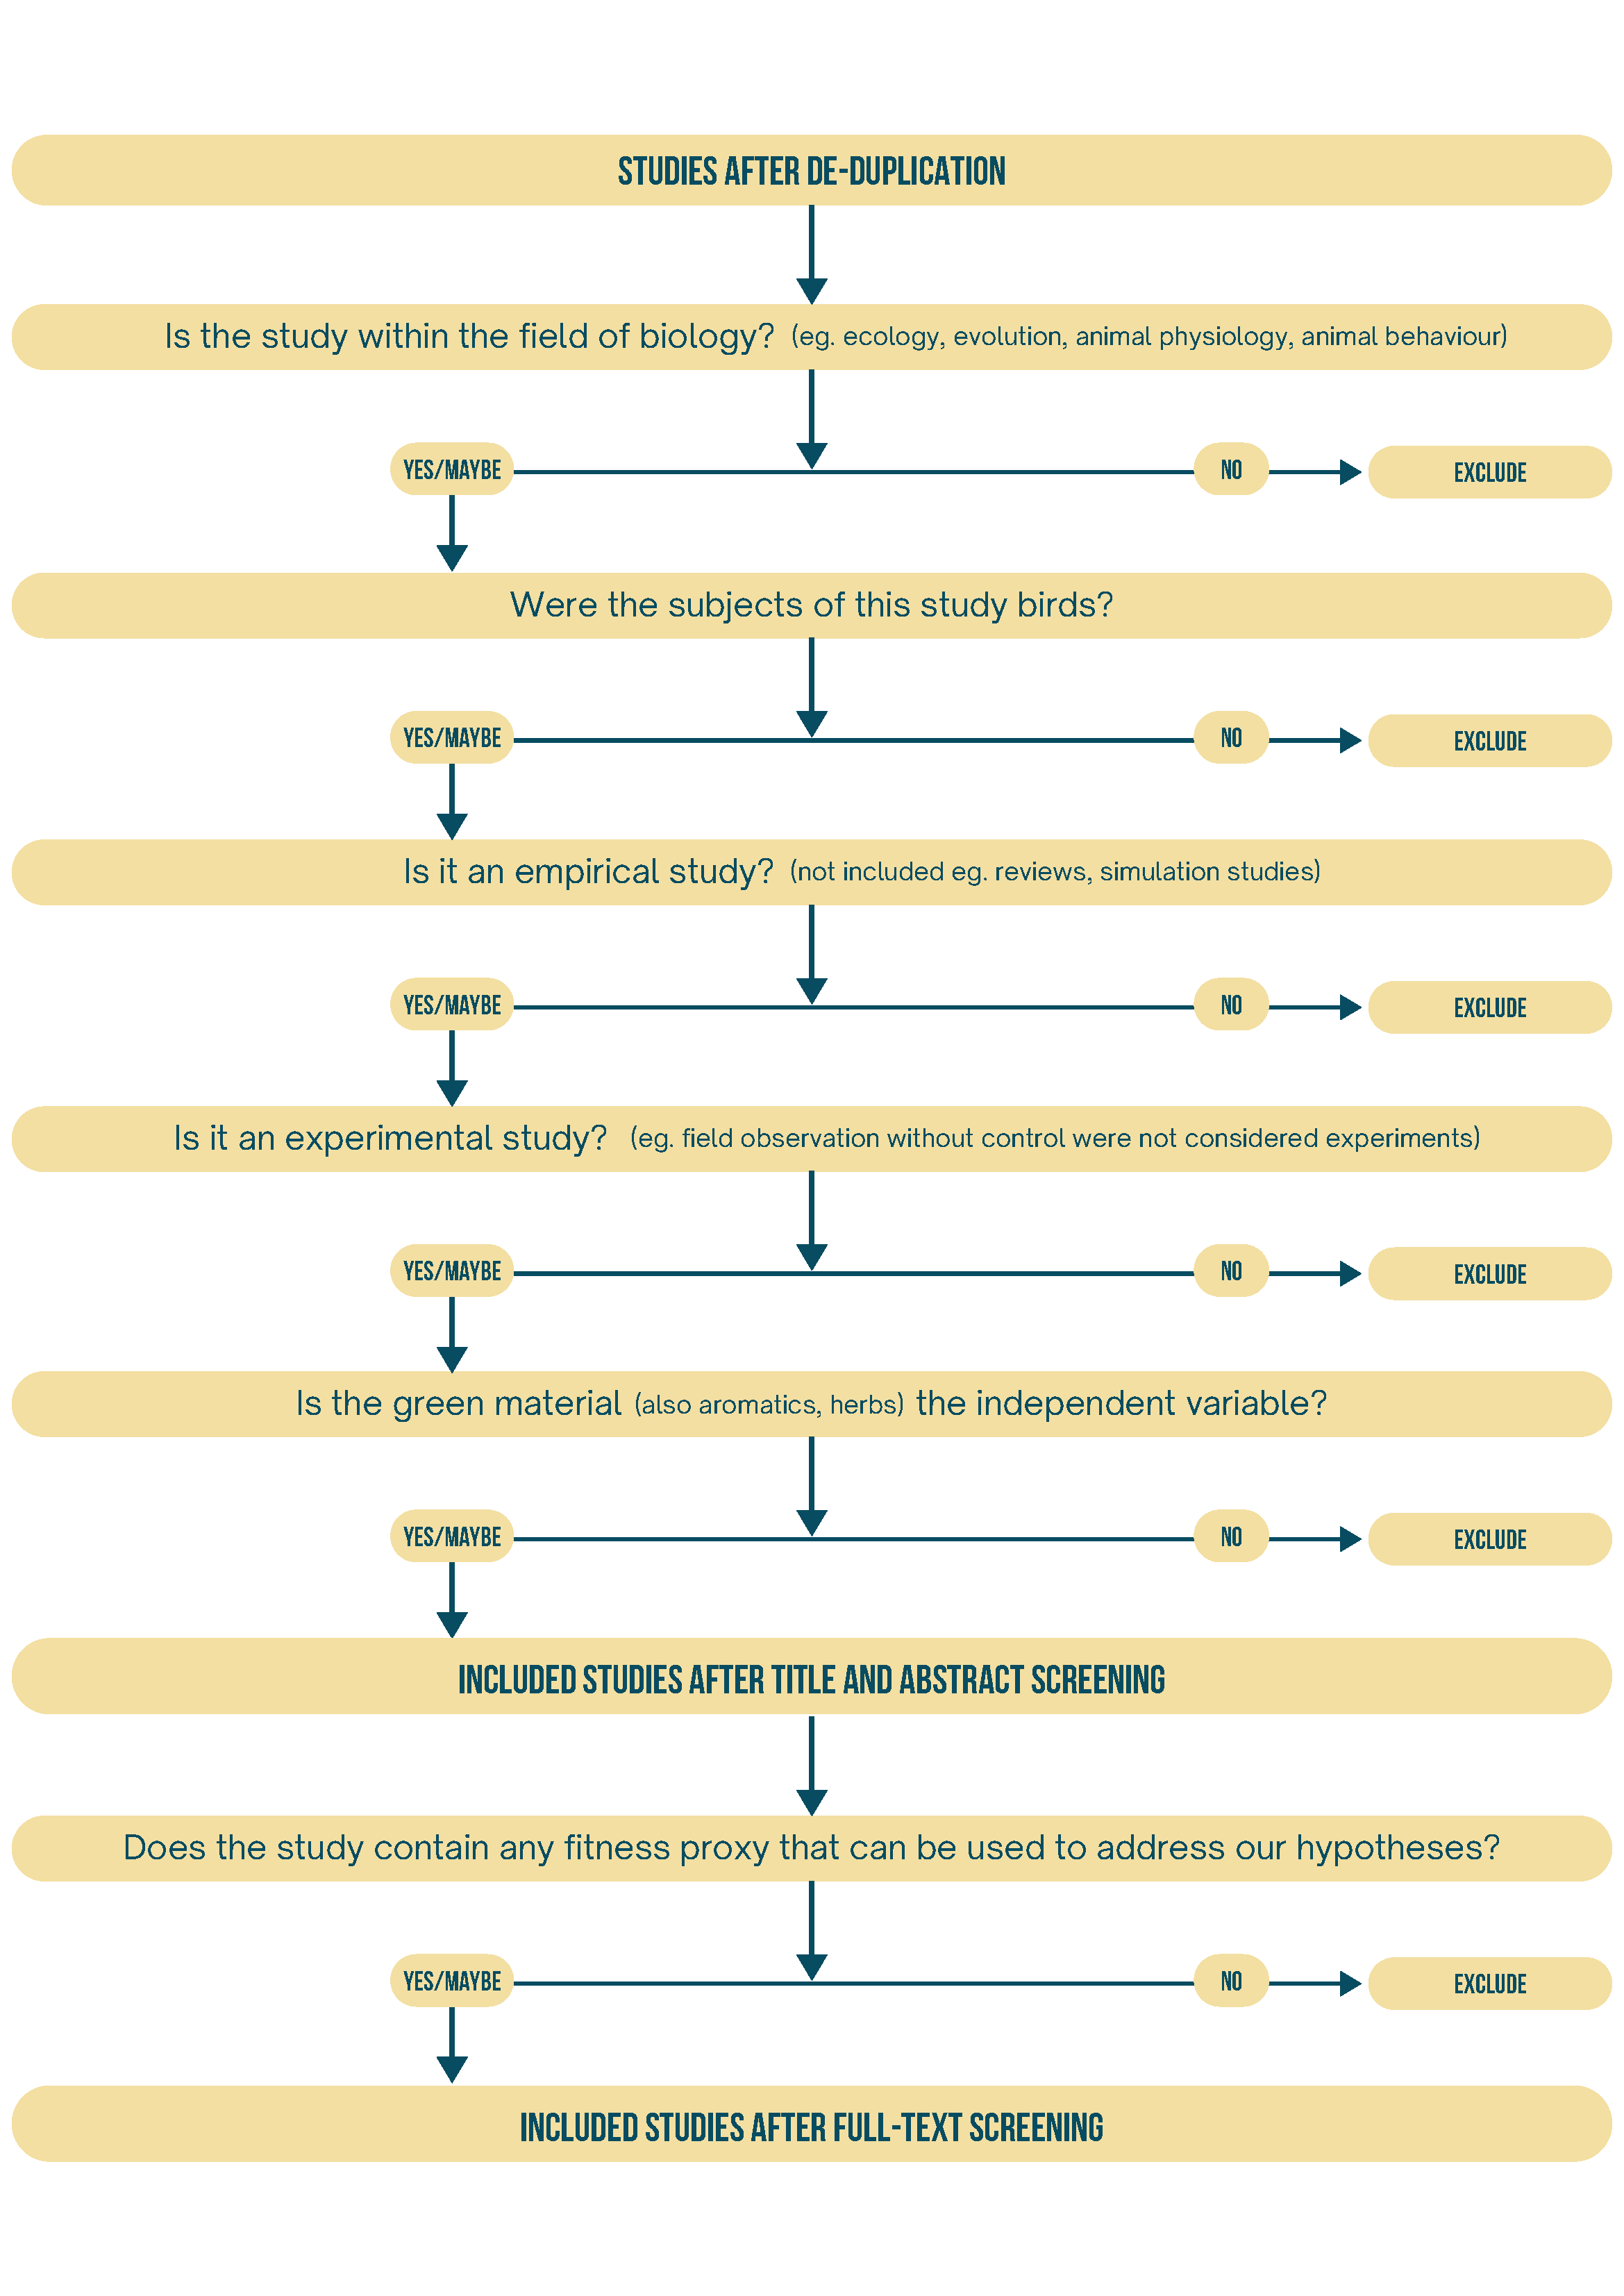
\includegraphics[width=0.8\linewidth,height=\textheight,keepaspectratio]{figures/Decision_Tree_updated.png}

\caption{\label{figsupp-decision-tree}\textbf{Decision tree used for
screening studies during title--abstract and full-text screening
process:}\\
The diagram illustrates the stepwise inclusion and exclusion criteria
applied to each article during screenings. At each decision point,
reviewers selected \emph{include/uncertain} or \emph{exclude}, following
pre-registered criteria to ensure consistency.}

\end{figsupp}%

\subsection{Fitness proxies included in the
meta-analysis}\label{fitness-proxies-included-in-the-meta-analysis}

\begin{figsupp}

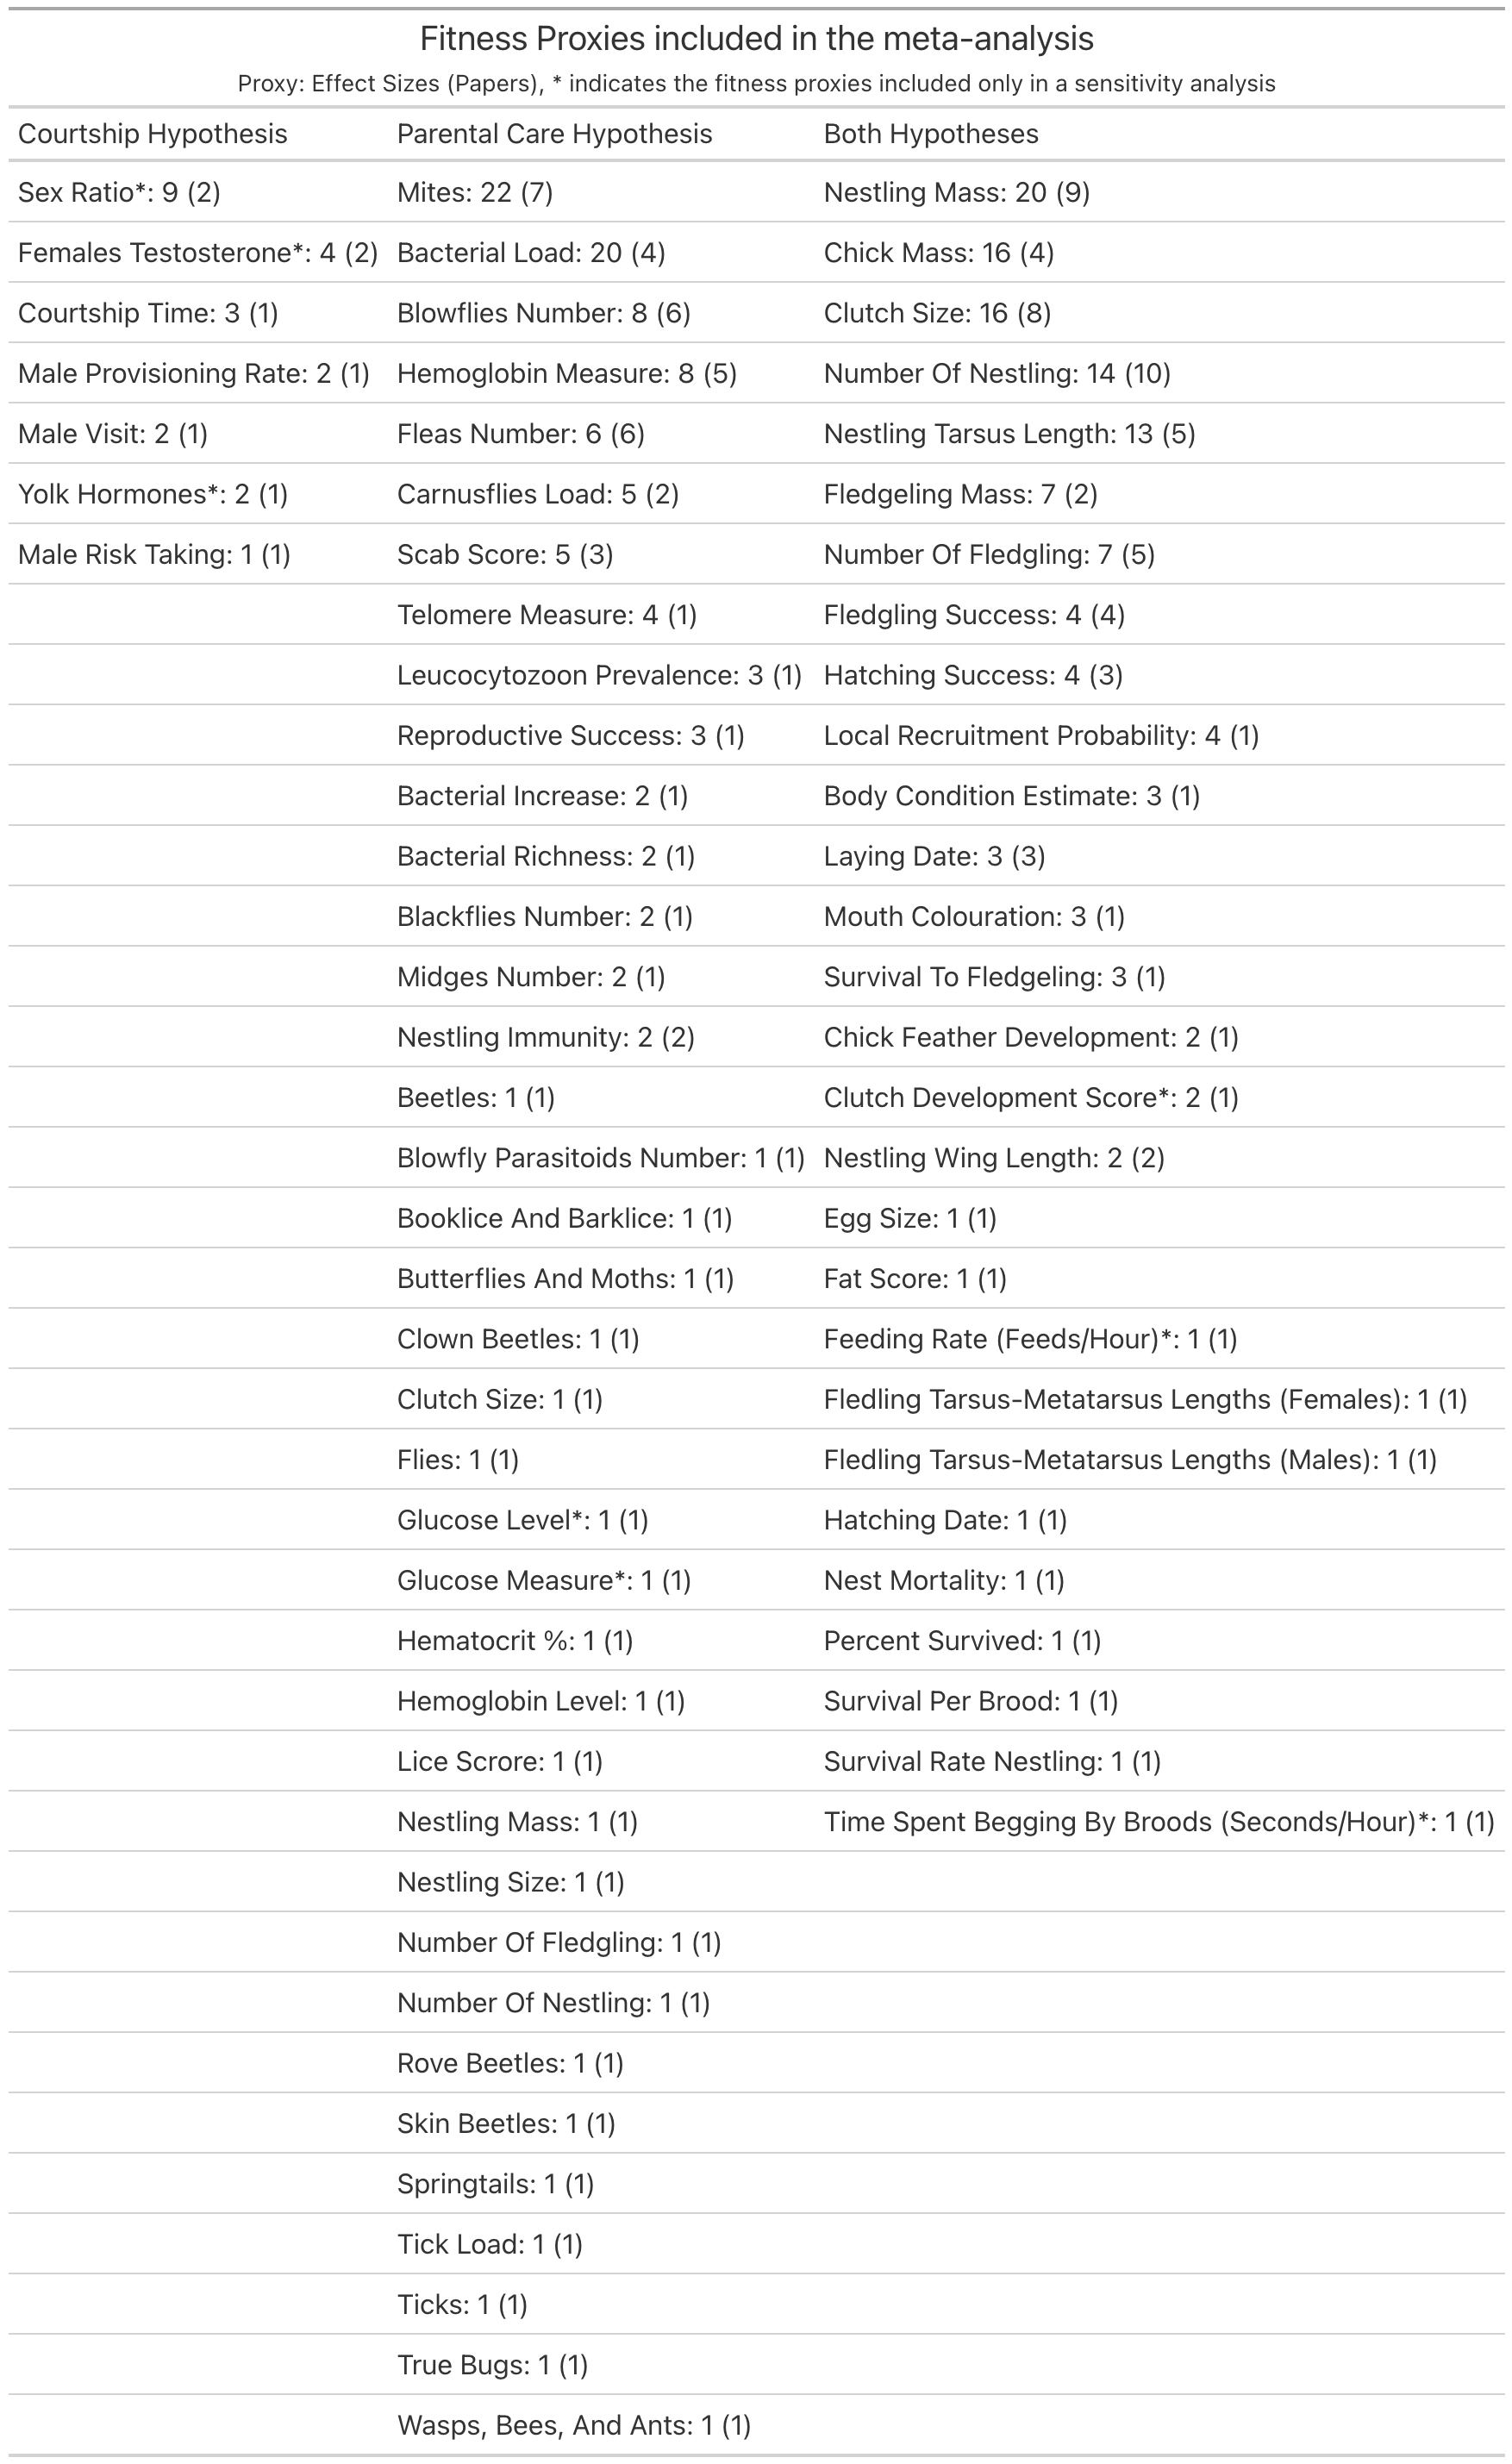
\includegraphics[width=0.7\linewidth,height=\textheight,keepaspectratio]{tables/SA_fitness_proxies_table.png}

\caption{\label{figsupp-fitness-proxies}\textbf{Summary of all fitness
proxies included in the meta-analysis}: Each column represents a
hypothesis tested in the dataset---Courtship Hypothesis, Parental Care
Hypothesis, and Both Hypotheses (studies addressing both). Entries list
each unique fitness proxy followed by the number of effect sizes (k,
numbers without brackets) and unique articles (n, numbers within
brackets) contributing data, formatted as Proxy: k(n). Proxies marked
with an asterisk (*) were included only in sensitivity analyses and not
in the main meta-analytic models.}

\end{figsupp}%

\subsection{Fitness proxies that were excluded from our
meta-analysis}\label{fitness-proxies-that-were-excluded-from-our-meta-analysis}

\begin{figsupp}

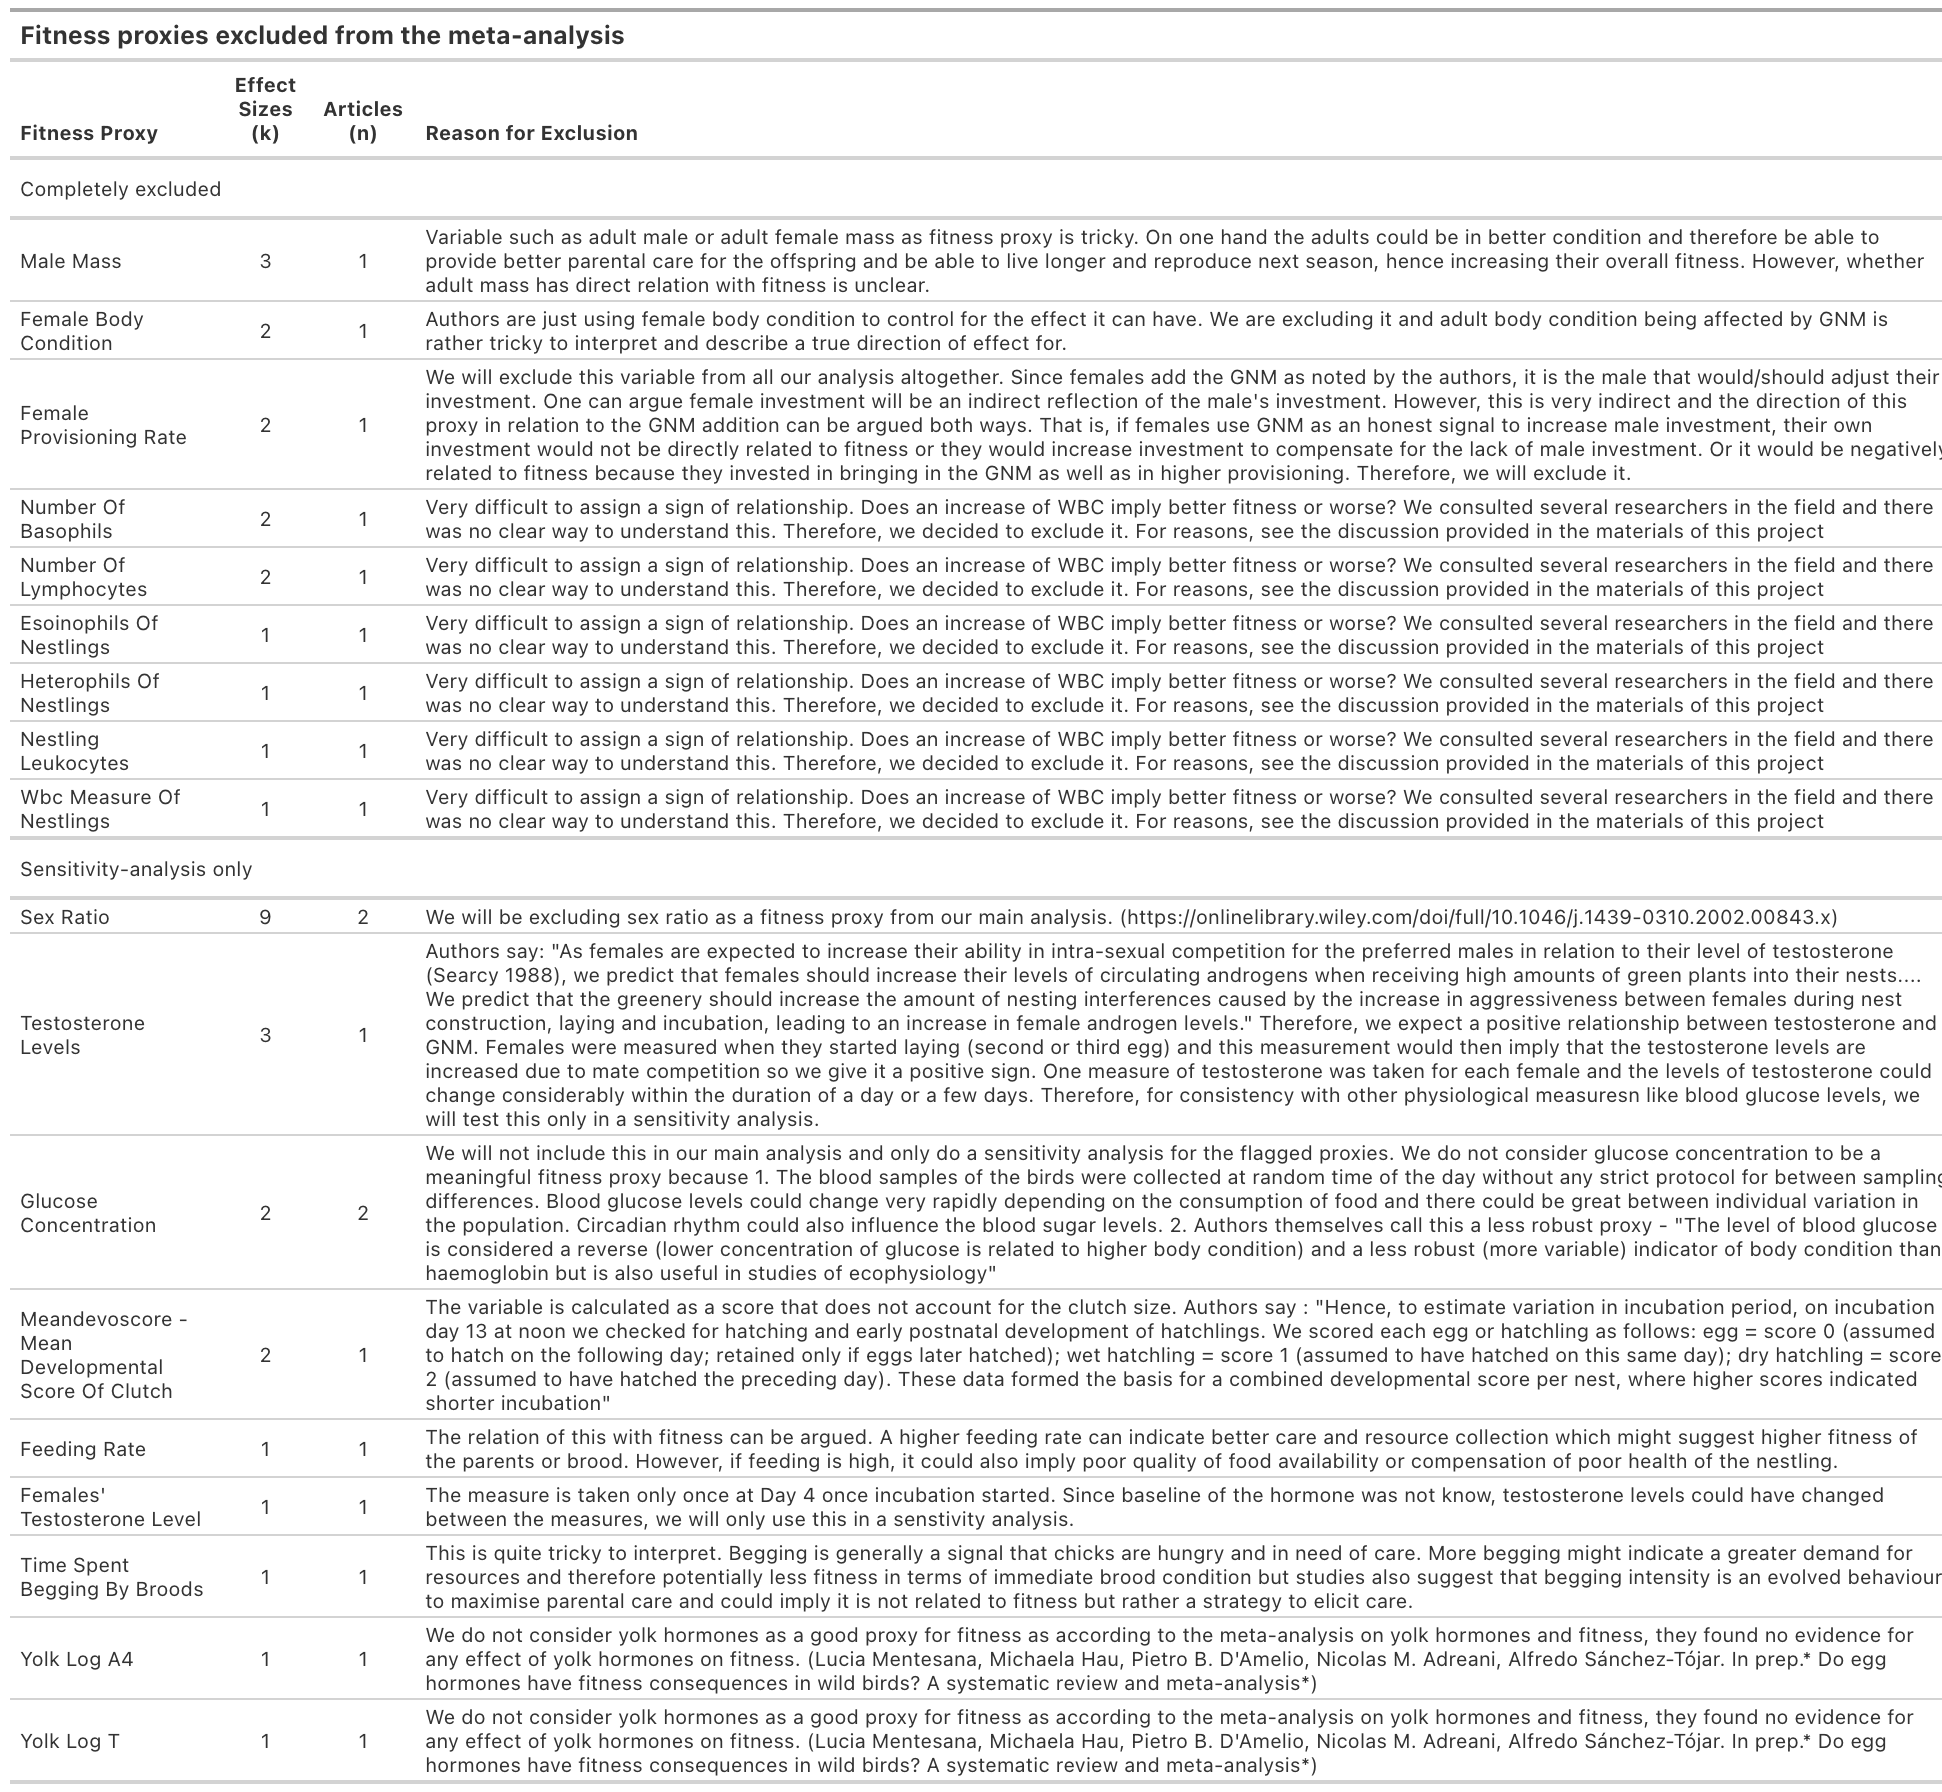
\includegraphics[width=0.9\linewidth,height=\textheight,keepaspectratio]{tables/SA_excluded_proxies_table.png}

\caption{\label{figsupp-excluded-proxies}\textbf{Summary of fitness
proxies completely removed from the meta-analysis or used only in
sensitivity analyses}: Fitness proxies were excluded when they could not
be assigned a consistent directional link to fitness or when the
literature on the validity of a proxy for fitness is highly debated.
``Completely excluded'' proxies were omitted from all models, whereas
``Sensitivity-analysis only'' proxies were tested separately to evaluate
the robustness of the meta-analytic results. Values denote the number of
effect sizes (k) and number of studies (n) for each proxy.}

\end{figsupp}%

\subsection{Standardized Email
Template}\label{standardized-email-template}

\begin{figsupp}

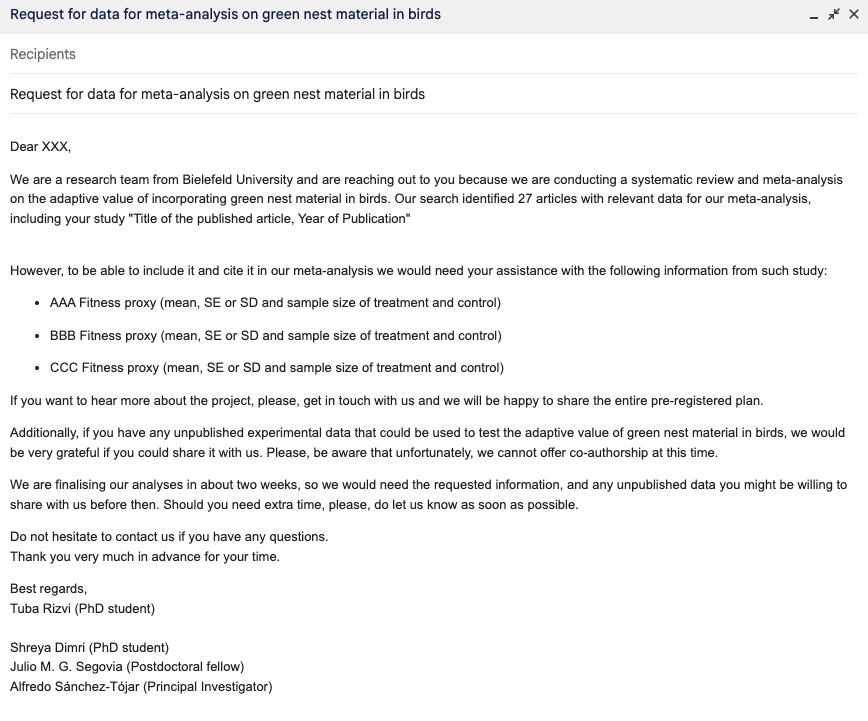
\includegraphics[width=0.8\linewidth,height=\textheight,keepaspectratio]{images/standardized-email-template.png}

\caption{\label{figsupp-email}\textbf{Standardized email template sent
to all the authors whose article was included in the meta-analysis}: In
cases where we needed the incomplete information, the fitness proxies of
interest were mentioned. In all cases, we requested for any unpublished
experimental data that could be used for the purpose of our
meta-analysis}

\end{figsupp}%

\begin{figsupp}

\centering{

\subsection{Description of Unpublished
studies}\label{description-of-unpublished-studies}

}

\caption{\label{figsupp-unpublished-study}}

\end{figsupp}%

We included two unpublished studies in our meta-analysis:

\paragraph{GNM\_1\_Unpublished:}\label{gnm_1_unpublished}

Greenery manipulation experiment was conducted over two breeding seasons
in 2018 and 2019. There were four treatment groups: Control, Spruce,
Plastic (Branches of an artificial Christmas tree) and Greenery removal.
Nests assigned to the spruce and plastic treatments, were lined with
approximately ten twigs in such a way that the entire nest platform was
covered. At nests assigned to the greenery removal treatment, all fresh
greenery was carefully removed while the nest structure was left
untouched. Greenery removal treatment was conditioned on the existence
of fresh greenery at the first sampling occasion. Control nests were
handled similarly but the greenery composition was not altered. For the
purpose of the meta-analysis we did not include the plastic treatment,
only, addition or removal of green material and control group. Sampling
interval was 5 to 19 days (mean: 7.72 ± 0.54, n = 42 nests).

Sample sizes 42 nests in total: 18 nests allocated to the spruce
treatment, 9 greenery removal, 10 plastic and 5 controls

Fitness proxies included in the meta-analysis:

\begin{enumerate}
\def\labelenumi{\arabic{enumi}.}
\item
  Body condition of the nestling
\item
  Ectoparasite load (Carnus hemapterus): Semi-quantitative measure with
  five levels, ranging from 0 (no infestation on any of the four
  locations) to 4 (C. hemapterus larvae or fresh biting marks present on
  all four examined body locations)
\item
  Endoparasite load (Leucocytozoon): Five levels 0 -- 4
\end{enumerate}

Data used for the meta-analysis can be found
data/02\_data\_extraction/data\_extraction\_MO\_checkedSD.xlsx\\

\paragraph{GNM\_2\_Unpublished:}\label{gnm_2_unpublished}

An experiment on Blue Tits conducted in Bergen (Norway), adding lavender
in nests and comparing nestling growth \& survival with controls. 5
fresh leaves of lavender were added / replaced every
2\textsuperscript{nd}day in broods in the ``aromatic'' group, from day 5
to day 13 after hatching. In the control group nothing was added, but
the broods were otherwise treated similarly.

The following variables were provided in the dataset:

\begin{enumerate}
\def\labelenumi{\arabic{enumi}.}
\tightlist
\item
  Weight D5, D7, D9, D11, D13 - Weight of nestlings at 5, 7, 9, 11, 13
  days after hatching of first egg
\item
  Weight D14-17 - Final weight measure on nestlings at days 14-17
  post-hatching, seen as fledging weight
\item
  TarsusLength D14-17 - Tarsus length measured on nestlings at days
  14-17 post-hatching, 0.1mm accuracy
\item
  Percent Survived - Percentage of all chicks initially hatched in each
  group that survived until fledging (therefore no SD)
\item
  Survival Per Brood - Percentage of chicks in each brood that survived
  until fledging (the unit is the brood here)
\end{enumerate}

This data was part of a Master thesis ``\textbf{Aromatic plants in nests
of blue tits (Cyanistes caeruleus)``} \citep{pantazi2024} and all the
details can be found at \url{https://hdl.handle.net/11250/3172874}.

Data used for the meta-analysis can be found
data/02\_data\_extraction/data\_extraction\_UnpublishedThesis.xlsx\\

\subsection{Complete List of Variables extracted from each
study}\label{complete-list-of-variables-extracted-from-each-study}

\begin{figsupp}

\centering{

Complete list of variables extracted from each study: comprehensive
overview of all variables recorded during data extraction.

}

\caption{\label{figsupp-variables}}

\end{figsupp}%

\begin{itemize}
\item
  Authors Complete information of all authors. Each author name to be
  separated by ;. Example: Dave Shutler and Adam A. Campbell → ``Shutler
  D; Campbell A A''.
\item
  Year of Publication The year the article was published.
\item
  Population Location Geographical location of the study population
  extracted as provided by the authors along with any coordinates
  provided. If multiple sites are studied in a location, extract them as
  PopulationName\_SiteA.
\item
  Experiment ID An identifier given to the estimates coming from the
  same sub-population within a location.
\item
  Group ID An identifier given to the estimates coming from the same
  group of experimental units (e.g., males and females in a population,
  first clutch and second clutch).
\item
  Repeated Trait ID An identifier given to the repeated measurement of
  the same trait within the same individuals (e.g., chick mass on day 7,
  14, and 21).
\item
  Bird Species Scientific name of the bird species studied.
\item
  Treatment Group Plant Species Scientific or common name of the plant
  species used as the green nest material (treatment group).
\item
  Control Group Plant Species Scientific name of the plant(s) species
  used as control treatment(s) in the study. If the scientific name is
  not given, extract it as reported by the authors. If there is no
  material used for control, note ``blank''.
\item
  Comparison Type Experimental design used to code the comparison
  between the two groups: 1 = non-aromatic (control) vs.~aromatic
  (treatment) 2 = no added material (control) vs.~aromatic (treatment) 3
  = no added material (control) vs.~non-aromatic (treatment)
\item
  CH Estimates related to the courtship hypothesis --- yes (1) or no
  (0).
\item
  PCH Estimates related to the nest protection or drug hypothesis ---
  yes (1) or no (0).
\item
  Measure of Central Tendency (treatment group) Estimated value of
  central tendency for the samples of the treatment group.
\item
  Type of Measure of Central Tendency (treatment group) Type of central
  tendency value reported for the treatment group (e.g., Mean, Median,
  Mode).
\item
  Measure of Dispersal (treatment group) Value of the measure of
  variation for the treatment group.
\item
  Type of Measure of Dispersal (treatment group) Type of variation of
  the data (e.g., SE, SD, CI95) reported for the treatment group.
\item
  Sample Size (treatment group) Sample size for the treatment group.
\item
  Measure of Central Tendency (control group) Estimated value of central
  tendency for the samples of the control group.
\item
  Type of Measure of Central Tendency (control group) Type of central
  tendency value reported for the control group (e.g., Mean, Median,
  Mode).
\item
  Measure of Dispersal (control group) Value of the measure of variation
  for the control group.
\item
  Type of Measure of Dispersal (control group) Type of variation of the
  data (e.g., SE, SD, CI95) reported for the control group.
\item
  Sample Size (control group) Sample size for the control group.
\item
  Fitness Proxy Measured Variable name used in the study as a proxy of
  fitness. Extracted as presented in the article and later standardized
  across studies.
\item
  Category/Type of Fitness Proxy Measured Type of trait (i.e., fitness
  proxy) studied: behaviour, morphology, parasite and pathogenic load,
  phenology, physiology, or reproduction.
\item
  Fitness Proxy Sign Sign assigned in relation to fitness: +1 if fitness
  increases with proxy (e.g., survival rate, body mass). −1 if fitness
  decreases with proxy (e.g., mortality, parasite load).
\item
  Statistics Type Type of statistics used to address the effect of GNM
  on fitness when primary data were not reported (e.g., t-test, ANOVA).
  Extracted only when central tendency was not reported.
\item
  Test Statistics Type Type of test statistic used (e.g., t, F).
\item
  Statistics Value Value of the test statistic used.
\item
  P Value Reported p-value (e.g., p = 0.003).
\item
  Sign Relationship Positive when treatment increases the trait value
  and negative when it decreases the trait value. Used when only the
  statistical value was provided.
\item
  Total Sample Size Total sample size used to calculate the statistical
  value.
\item
  Degree of Freedom Degrees of freedom for the statistics used.
\item
  Data Location The part of the text or figure from which the data were
  extracted.
\item
  Parasite Type Type of parasite when fitness proxy measured
  parasite/pathogen load (Arthropod or Micro-organism).
\item
  Time of Green Nest Material Addition Time of green nest material
  addition by authors or birds {[}continuous (c), before (b), or after
  (a) egg hatching{]}.
\item
  Blinding Whether blinding was conducted --- yes (y) or no (n).
\item
  Random Assignment Whether nests were assigned to treatment or control
  randomly --- yes (y) or no (n).
\item
  Missing Data Whether data were only partially or not reported --- yes
  (y) or no (n).
\item
  Shared Treatment Group Used to identify non-independence between
  shared treatment groups. Value = 1 if individuals were compared only
  once as a treatment group.
\item
  Shared Control Group Used to identify non-independence between shared
  control groups. Value = 1 if individuals were compared only once as a
  control group.
\end{itemize}

\subsection{Random Effects}\label{random-effects}

\begin{figsupp}

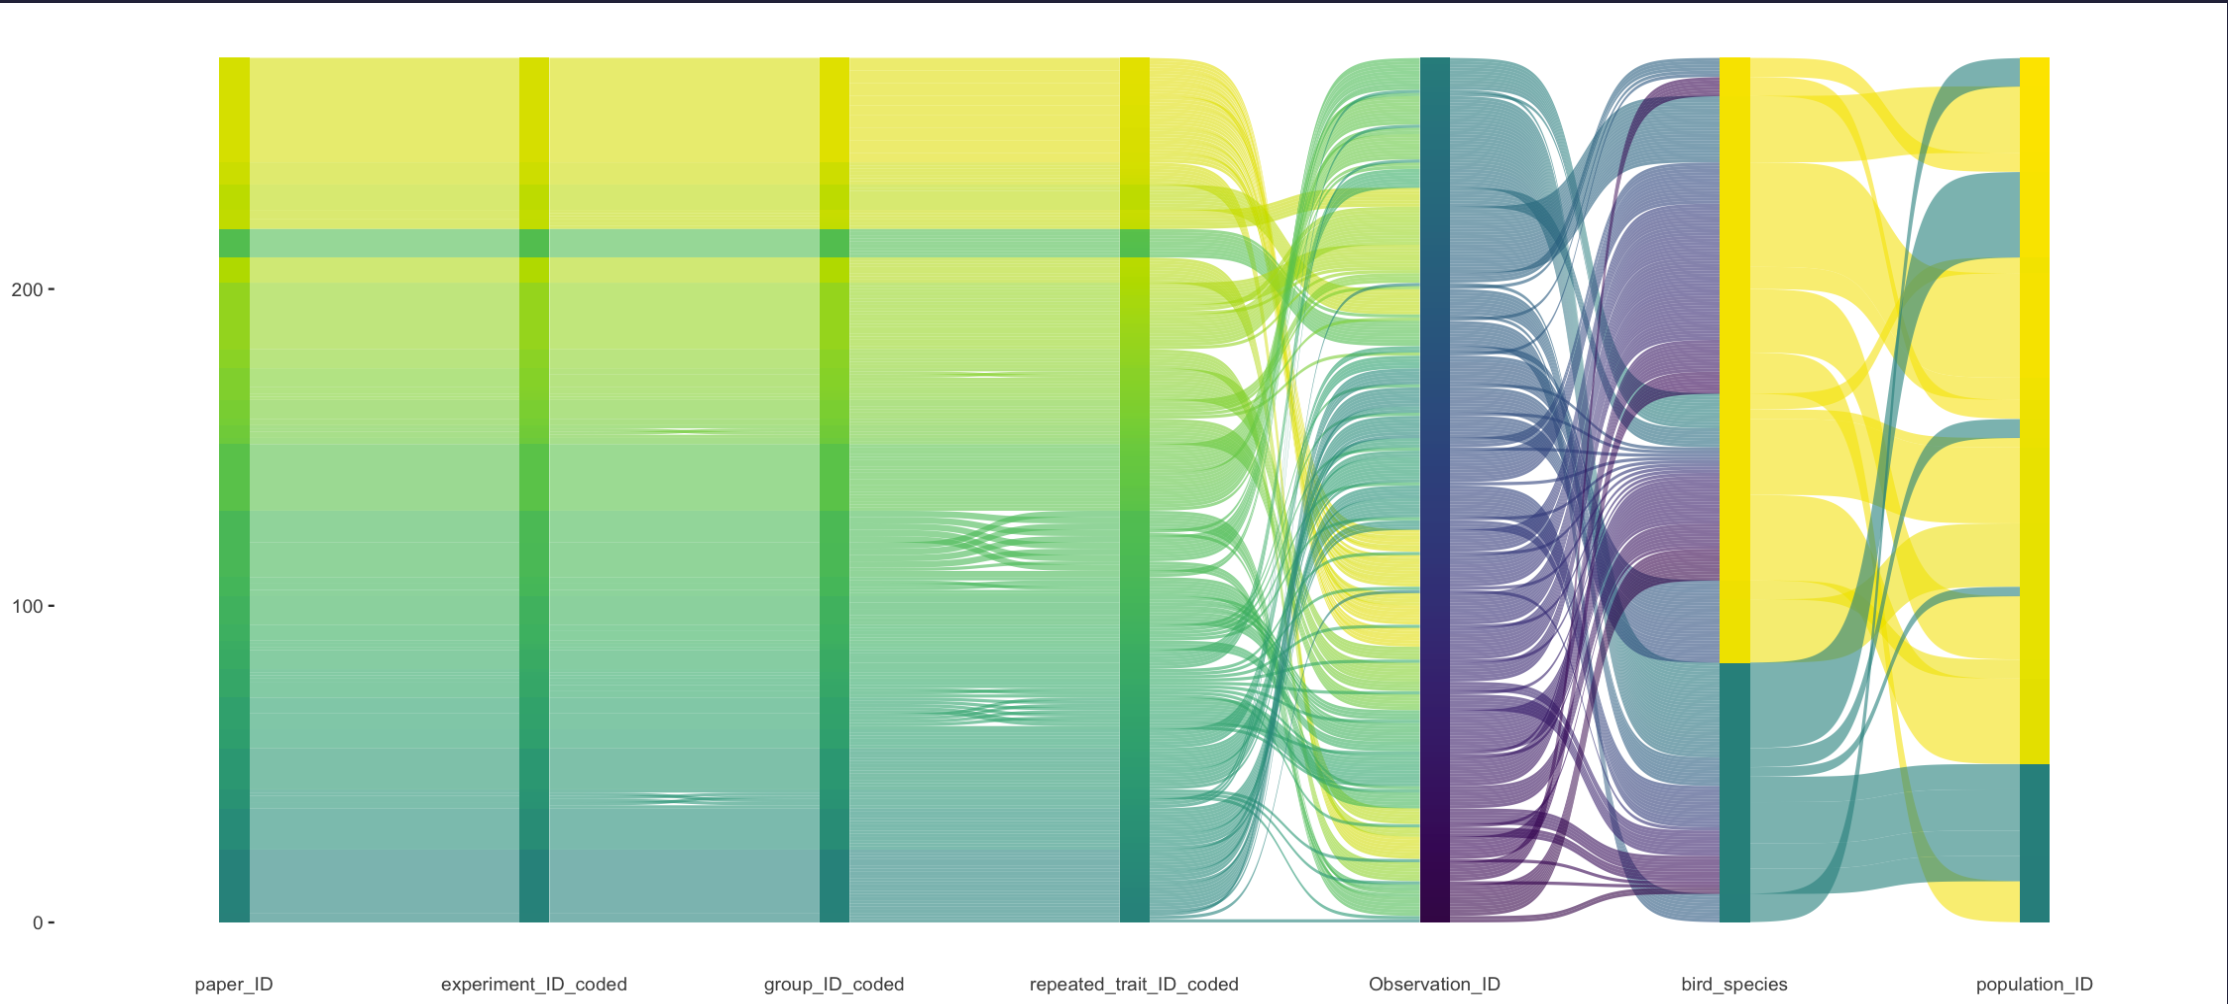
\includegraphics[width=0.9\linewidth,height=\textheight,keepaspectratio]{images/alluvial_random_effects.png}

\caption{\label{figsupp-random-effect}\textbf{Alluvial plot showing the
overlap among random effects extracted for the meta-analytic dataset:}
Each vertical bar represents a random-effect term i.e.~Paper ID (28
levels), Experiment ID (48), Group ID (52), Repeated Trait ID (225),
Observation ID (273), Bird Species (7), and Population ID (20).
Connections between bars indicate shared values across levels. The
figure shows that Experiment ID and Group ID were nearly identical, and
that Repeated Trait ID had many levels almost as many as the Observation
ID, and Repeated Trait ID was excluded from the final models. In
contrast, Population ID captured additional clustering across studies
and was therefore added to the random effects (not pre-registered).}

\end{figsupp}%

\subsection{Sensitivity analysis of sampling correlation values (ρ) in
variance--covariance
structures}\label{sensitivity-analysis-of-sampling-correlation-values-ux3c1-in-variancecovariance-structures}

\begin{figsupp}

\centering{

\pandocbounded{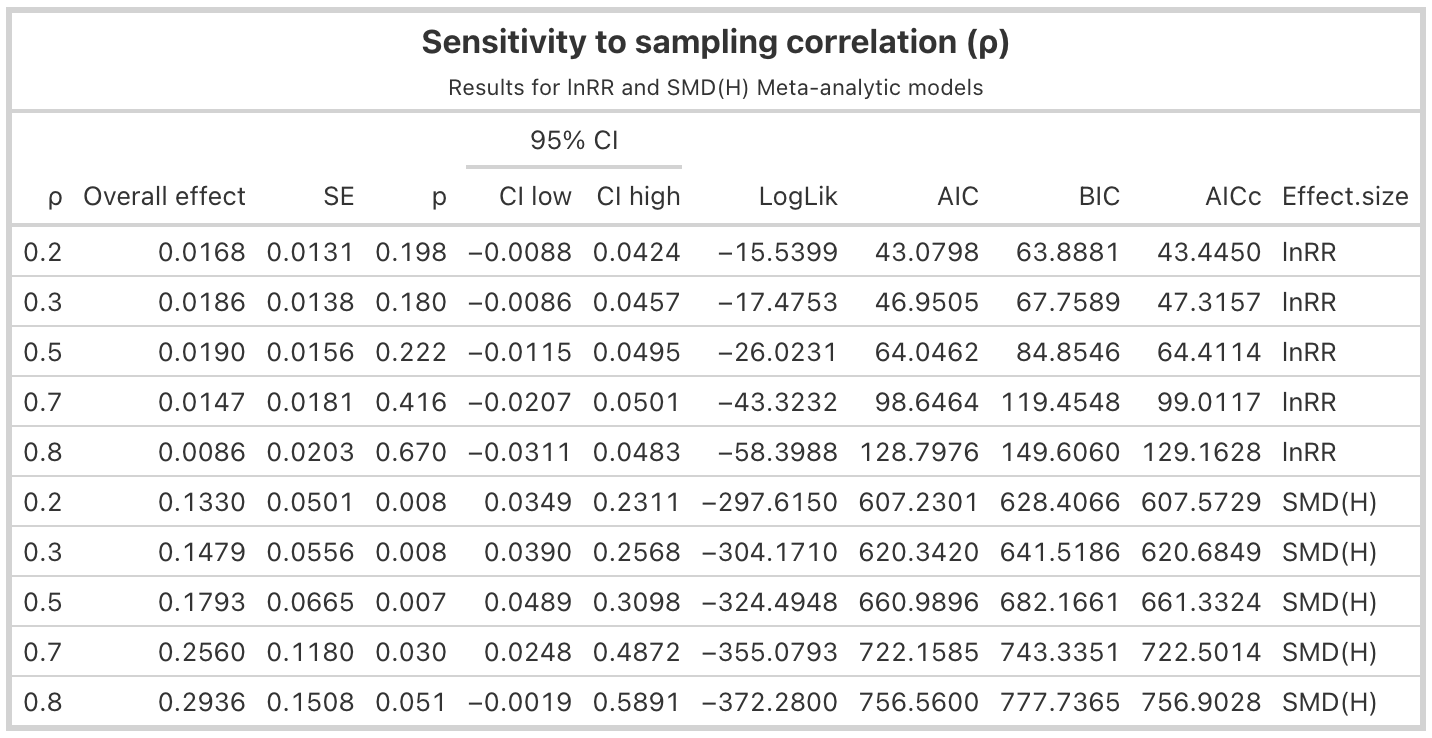
\includegraphics[keepaspectratio]{tables/SA_sampling-correlation_table.png}}

}

\caption{\label{figsupp-correlation}\textbf{Sensitivity of overall
effect estimates to the assumed sampling correlation (ρ):} The table
shows model estimates of the overall effect, standard errors (SE),
\emph{p}-values, 95\% confidence intervals (CI), and fit statistics
(log-likelihood, AIC, BIC, and AICc) across a range of assumed sampling
correlations (ρ) used for the variance-covariance matrices.}

\end{figsupp}%

\subsection{All sensitivity-analysis/robustness
check}\label{all-sensitivity-analysisrobustness-check}

\begin{tabsupp}

\centering{

\pandocbounded{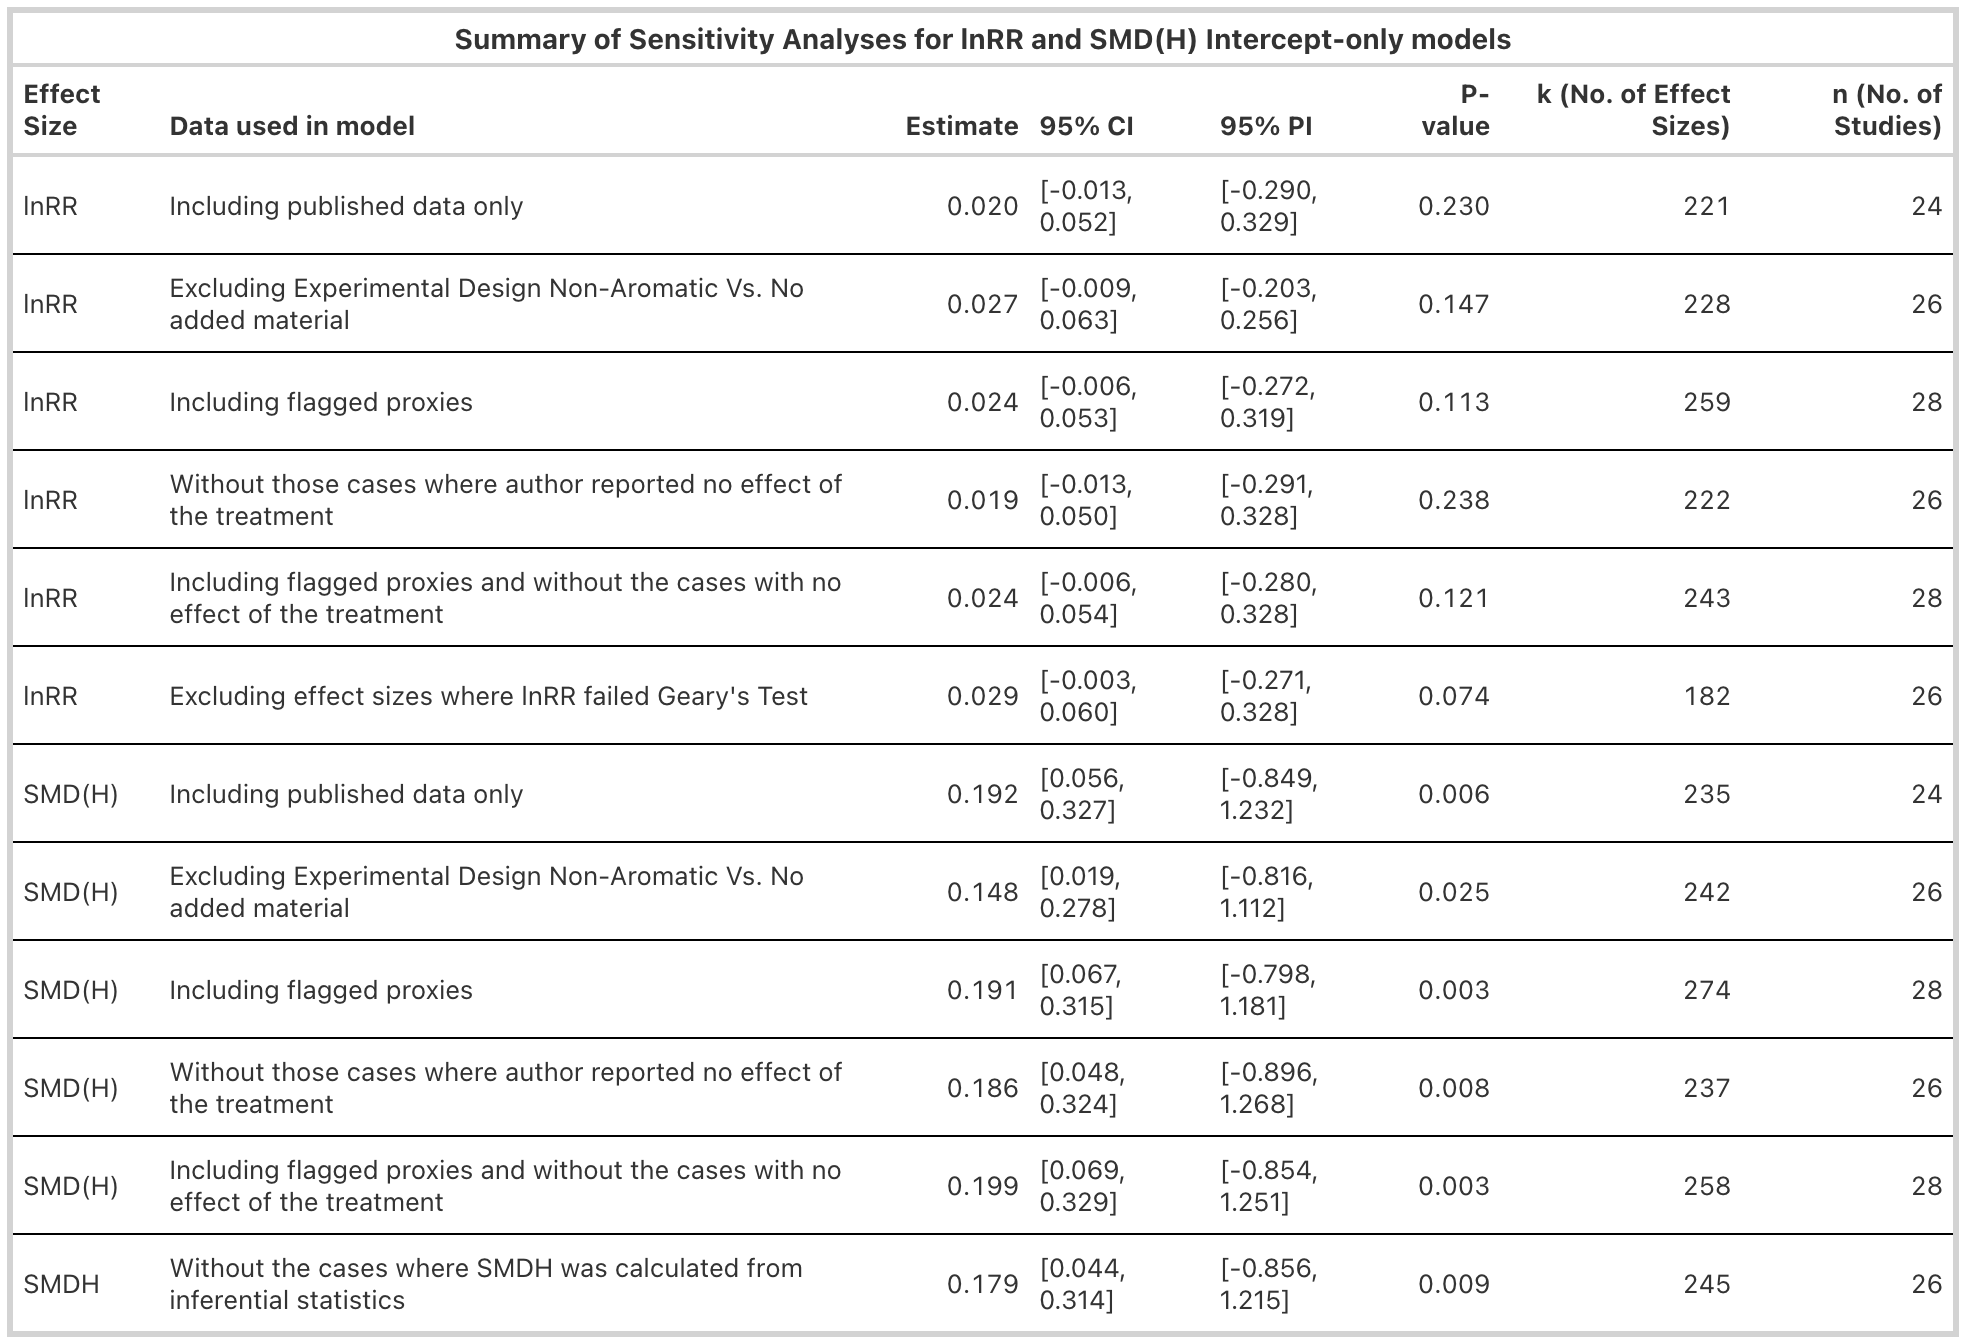
\includegraphics[keepaspectratio]{tables/SA_intercept_only.png}}

}

\caption{\label{tabsupp-SA-intercept}}

\end{tabsupp}%

\subsection{Plots without cropping the axis (showing complete
X-axis)}\label{plots-without-cropping-the-axis-showing-complete-x-axis}

\begin{figsupp}

\centering{

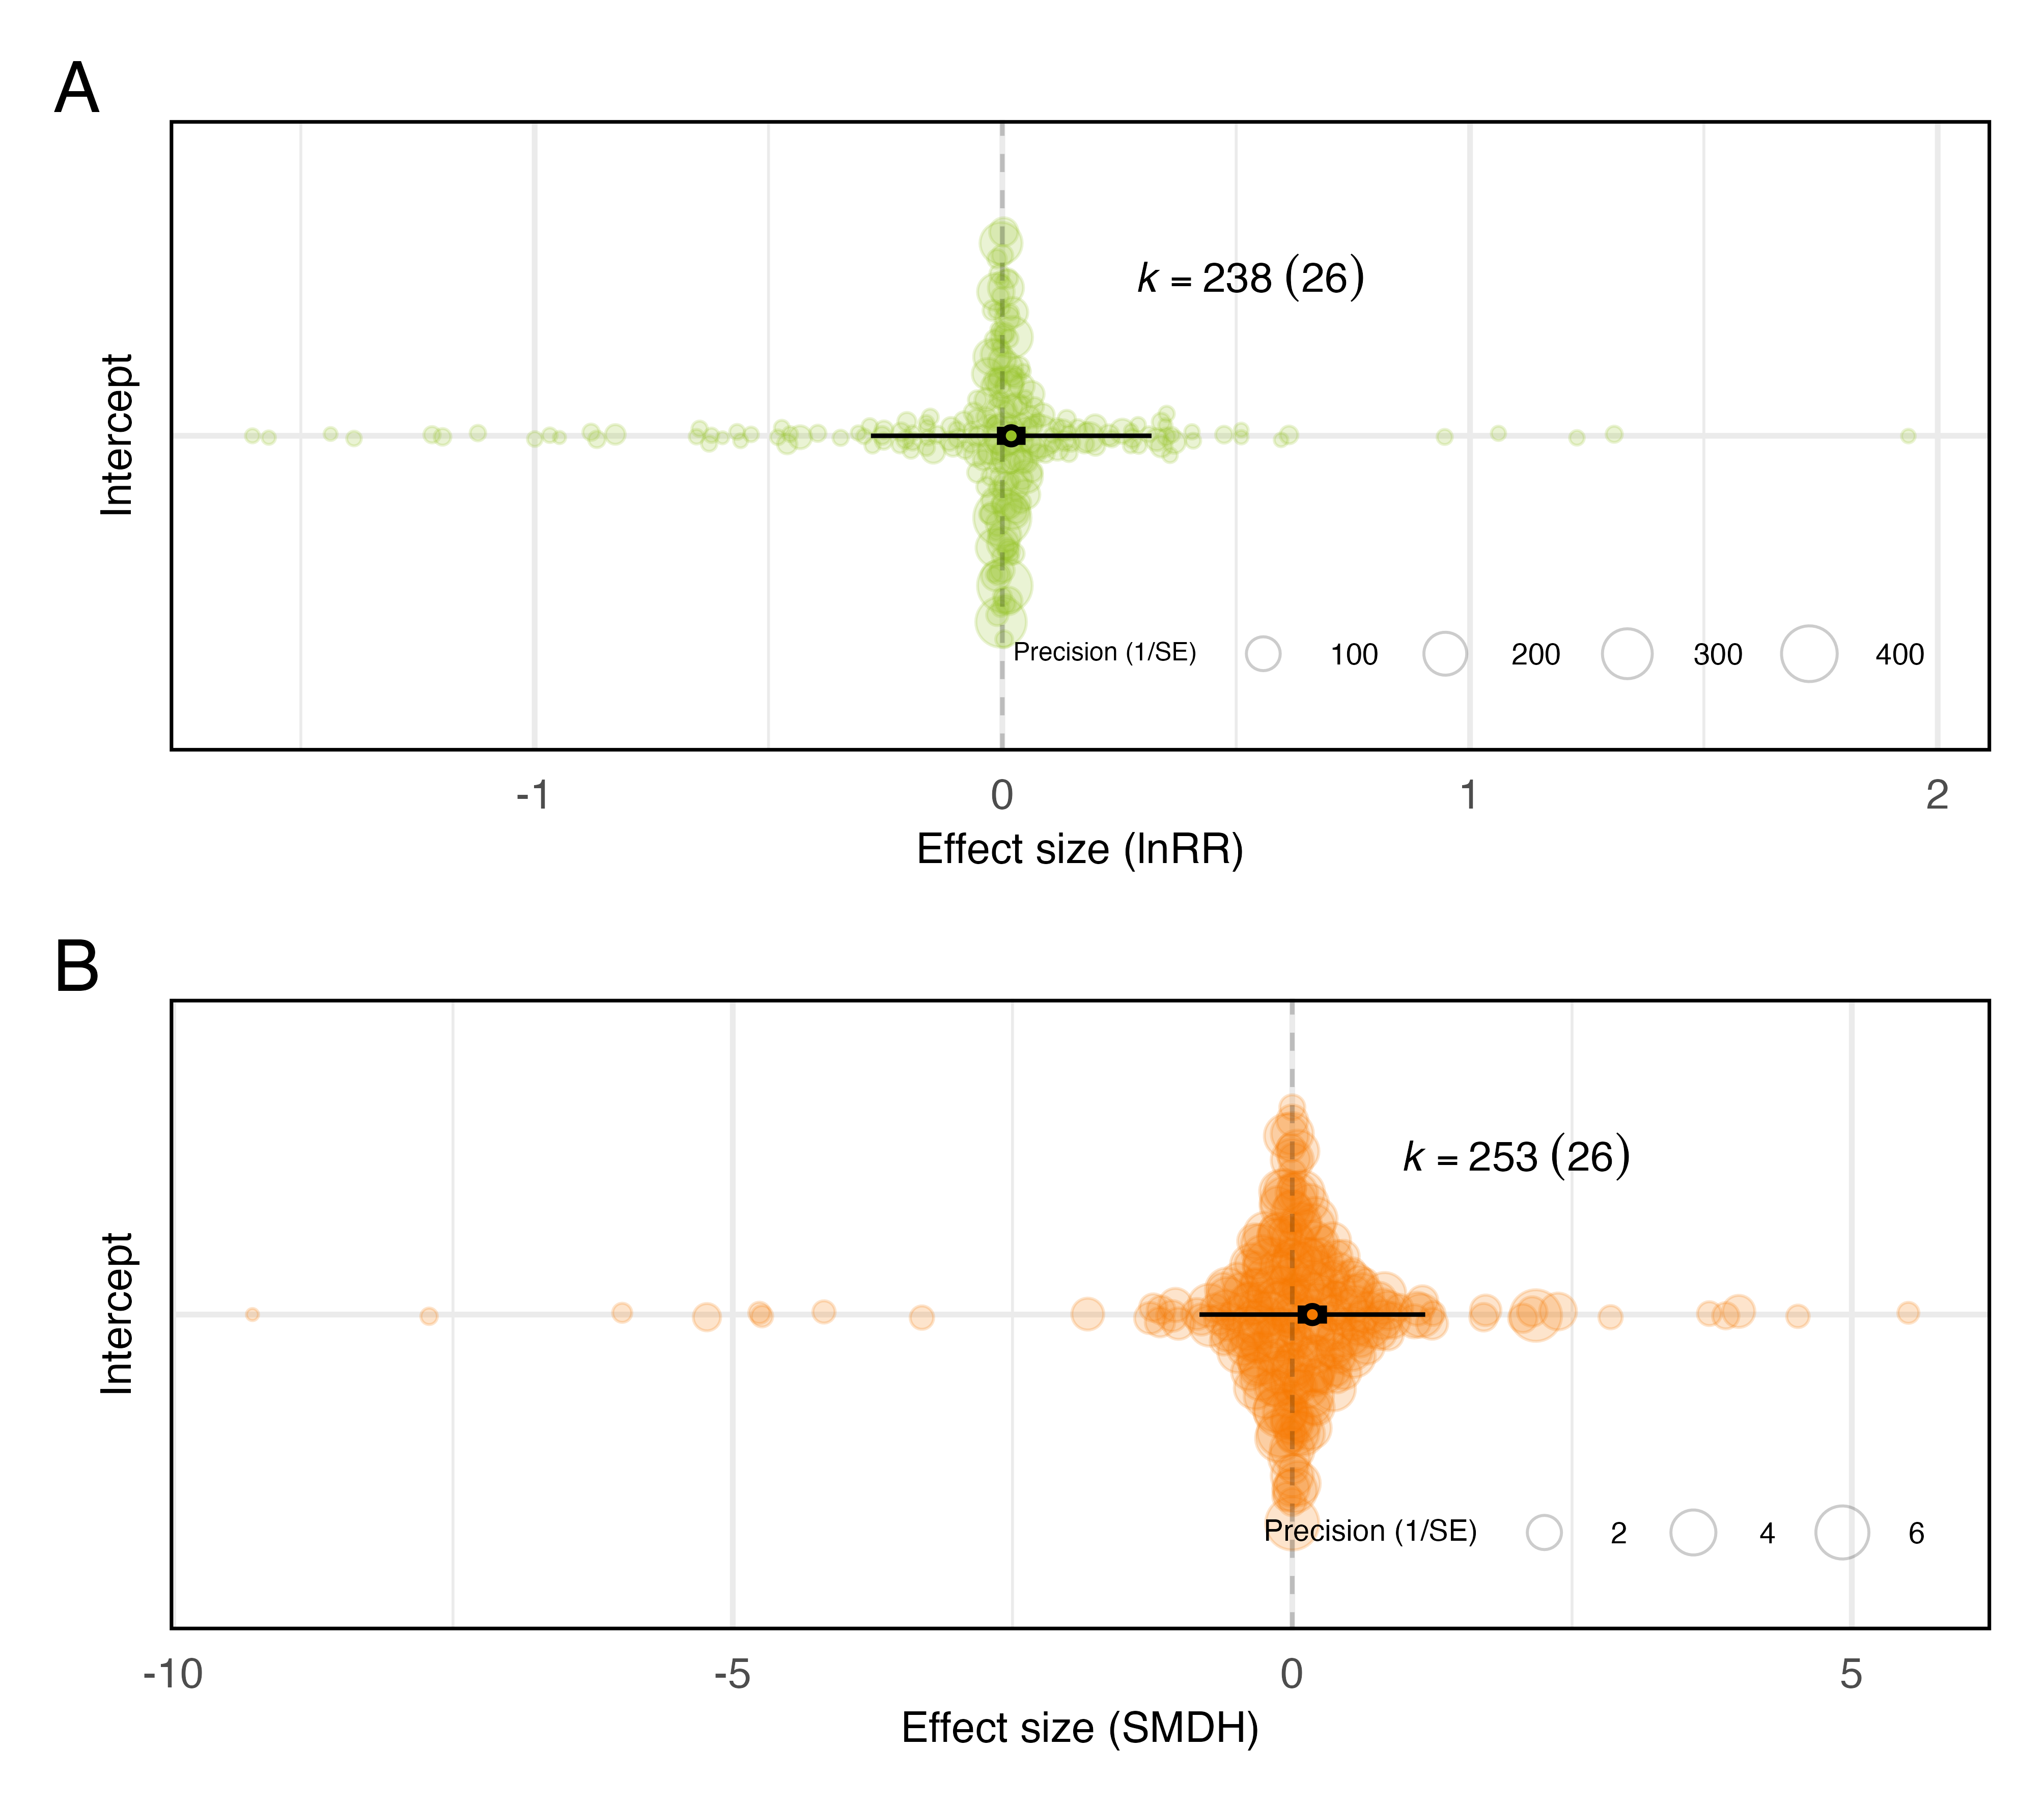
\includegraphics[width=0.9\linewidth,height=\textheight,keepaspectratio]{figures/Figure_overall_effect.png}

}

\caption{\label{figsupp-overall}Overall effect of green nest material on
all fitness proxies combined. The meta-analytic mean (black circle) with
95\% confidence intervals (thicker bars) and prediction intervals
(thinner bars) are shown along with the data points (coloured circles)
scaled by precision (inverse of standard error). Results are shown as an
orchard plot for the intercept-only model (A) using log response ratio
(lnRR), and (B) standardised mean difference (SMD(H)). k: number of
effect sizes (number of studies is shown in the brackets).}

\end{figsupp}%

\begin{figsupp}

\centering{

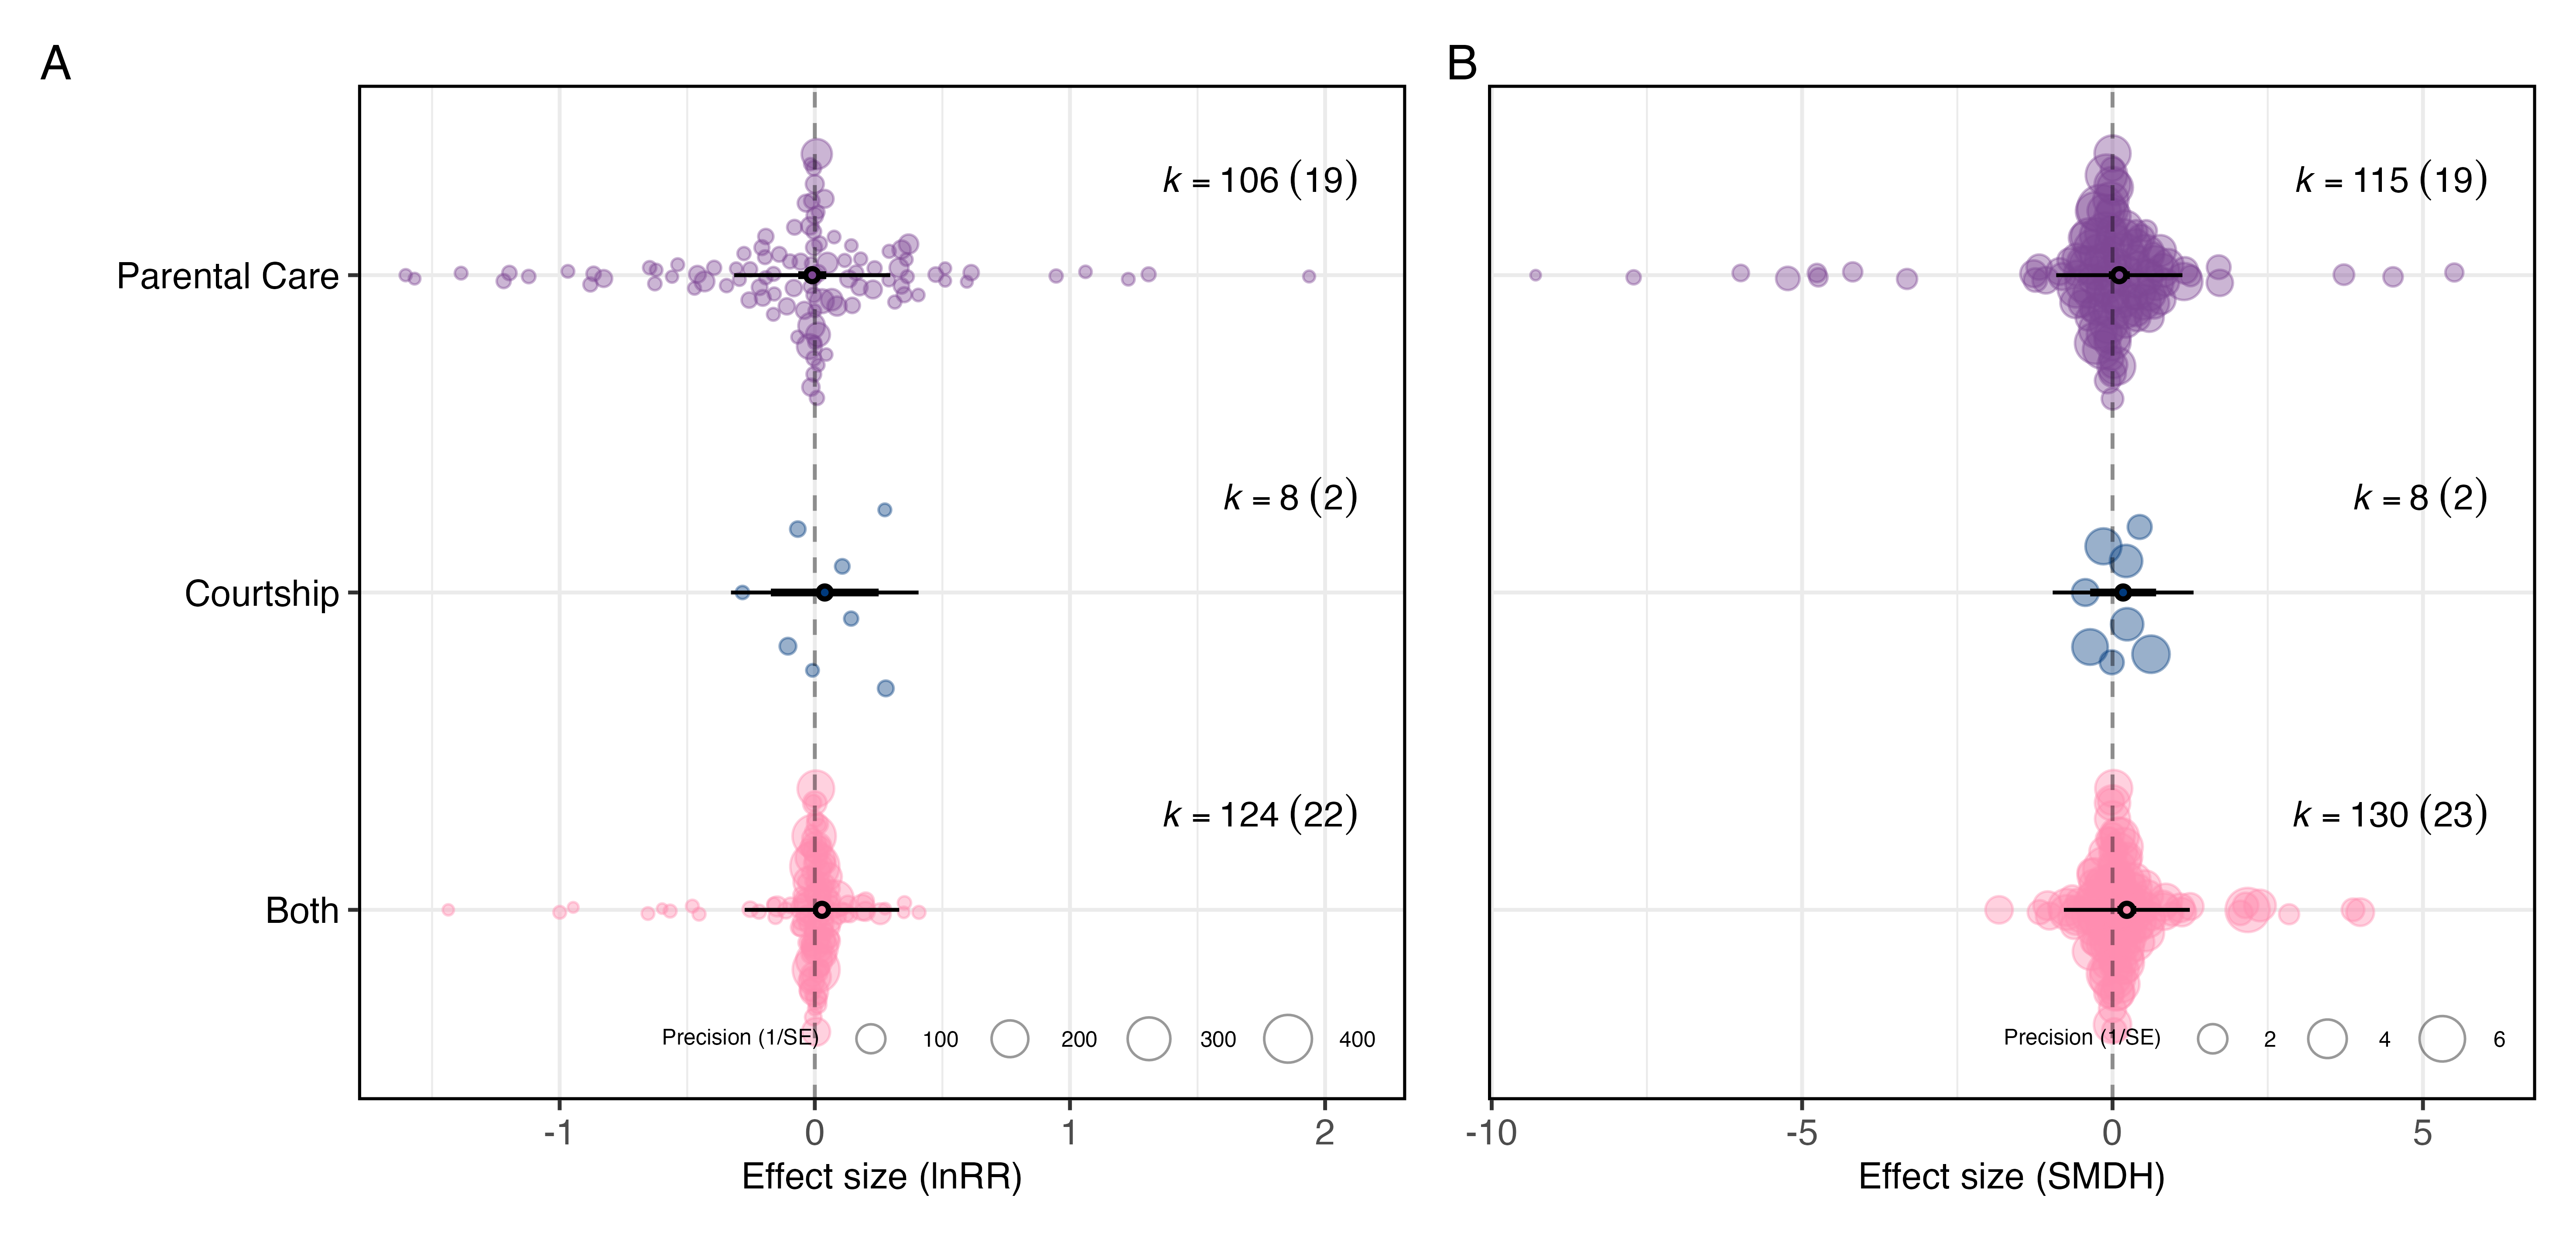
\includegraphics[width=0.9\linewidth,height=\textheight,keepaspectratio]{figures/Figure_hypothesis.png}

}

\caption{\label{figsupp-hypothesis}There is no clear evidence to favour
either the courtship or the parental care hypothesis as drivers of
potential fitness benefits of green nest material. Orchard plot of the
multilevel meta-regression for (A) log response ratio (lnRR) and (B)
standardised mean difference (SMD(H)). Mean estimates (black circles),
95\% confidence intervals (thicker bars), and prediction intervals
(thinner bars) are shown along with the individual data points
(transparently coloured circles) scaled by precision (inverse of
standard error). k: number of effect sizes (number of studies is shown
in the brackets).}

\end{figsupp}%

\begin{figsupp}

\centering{

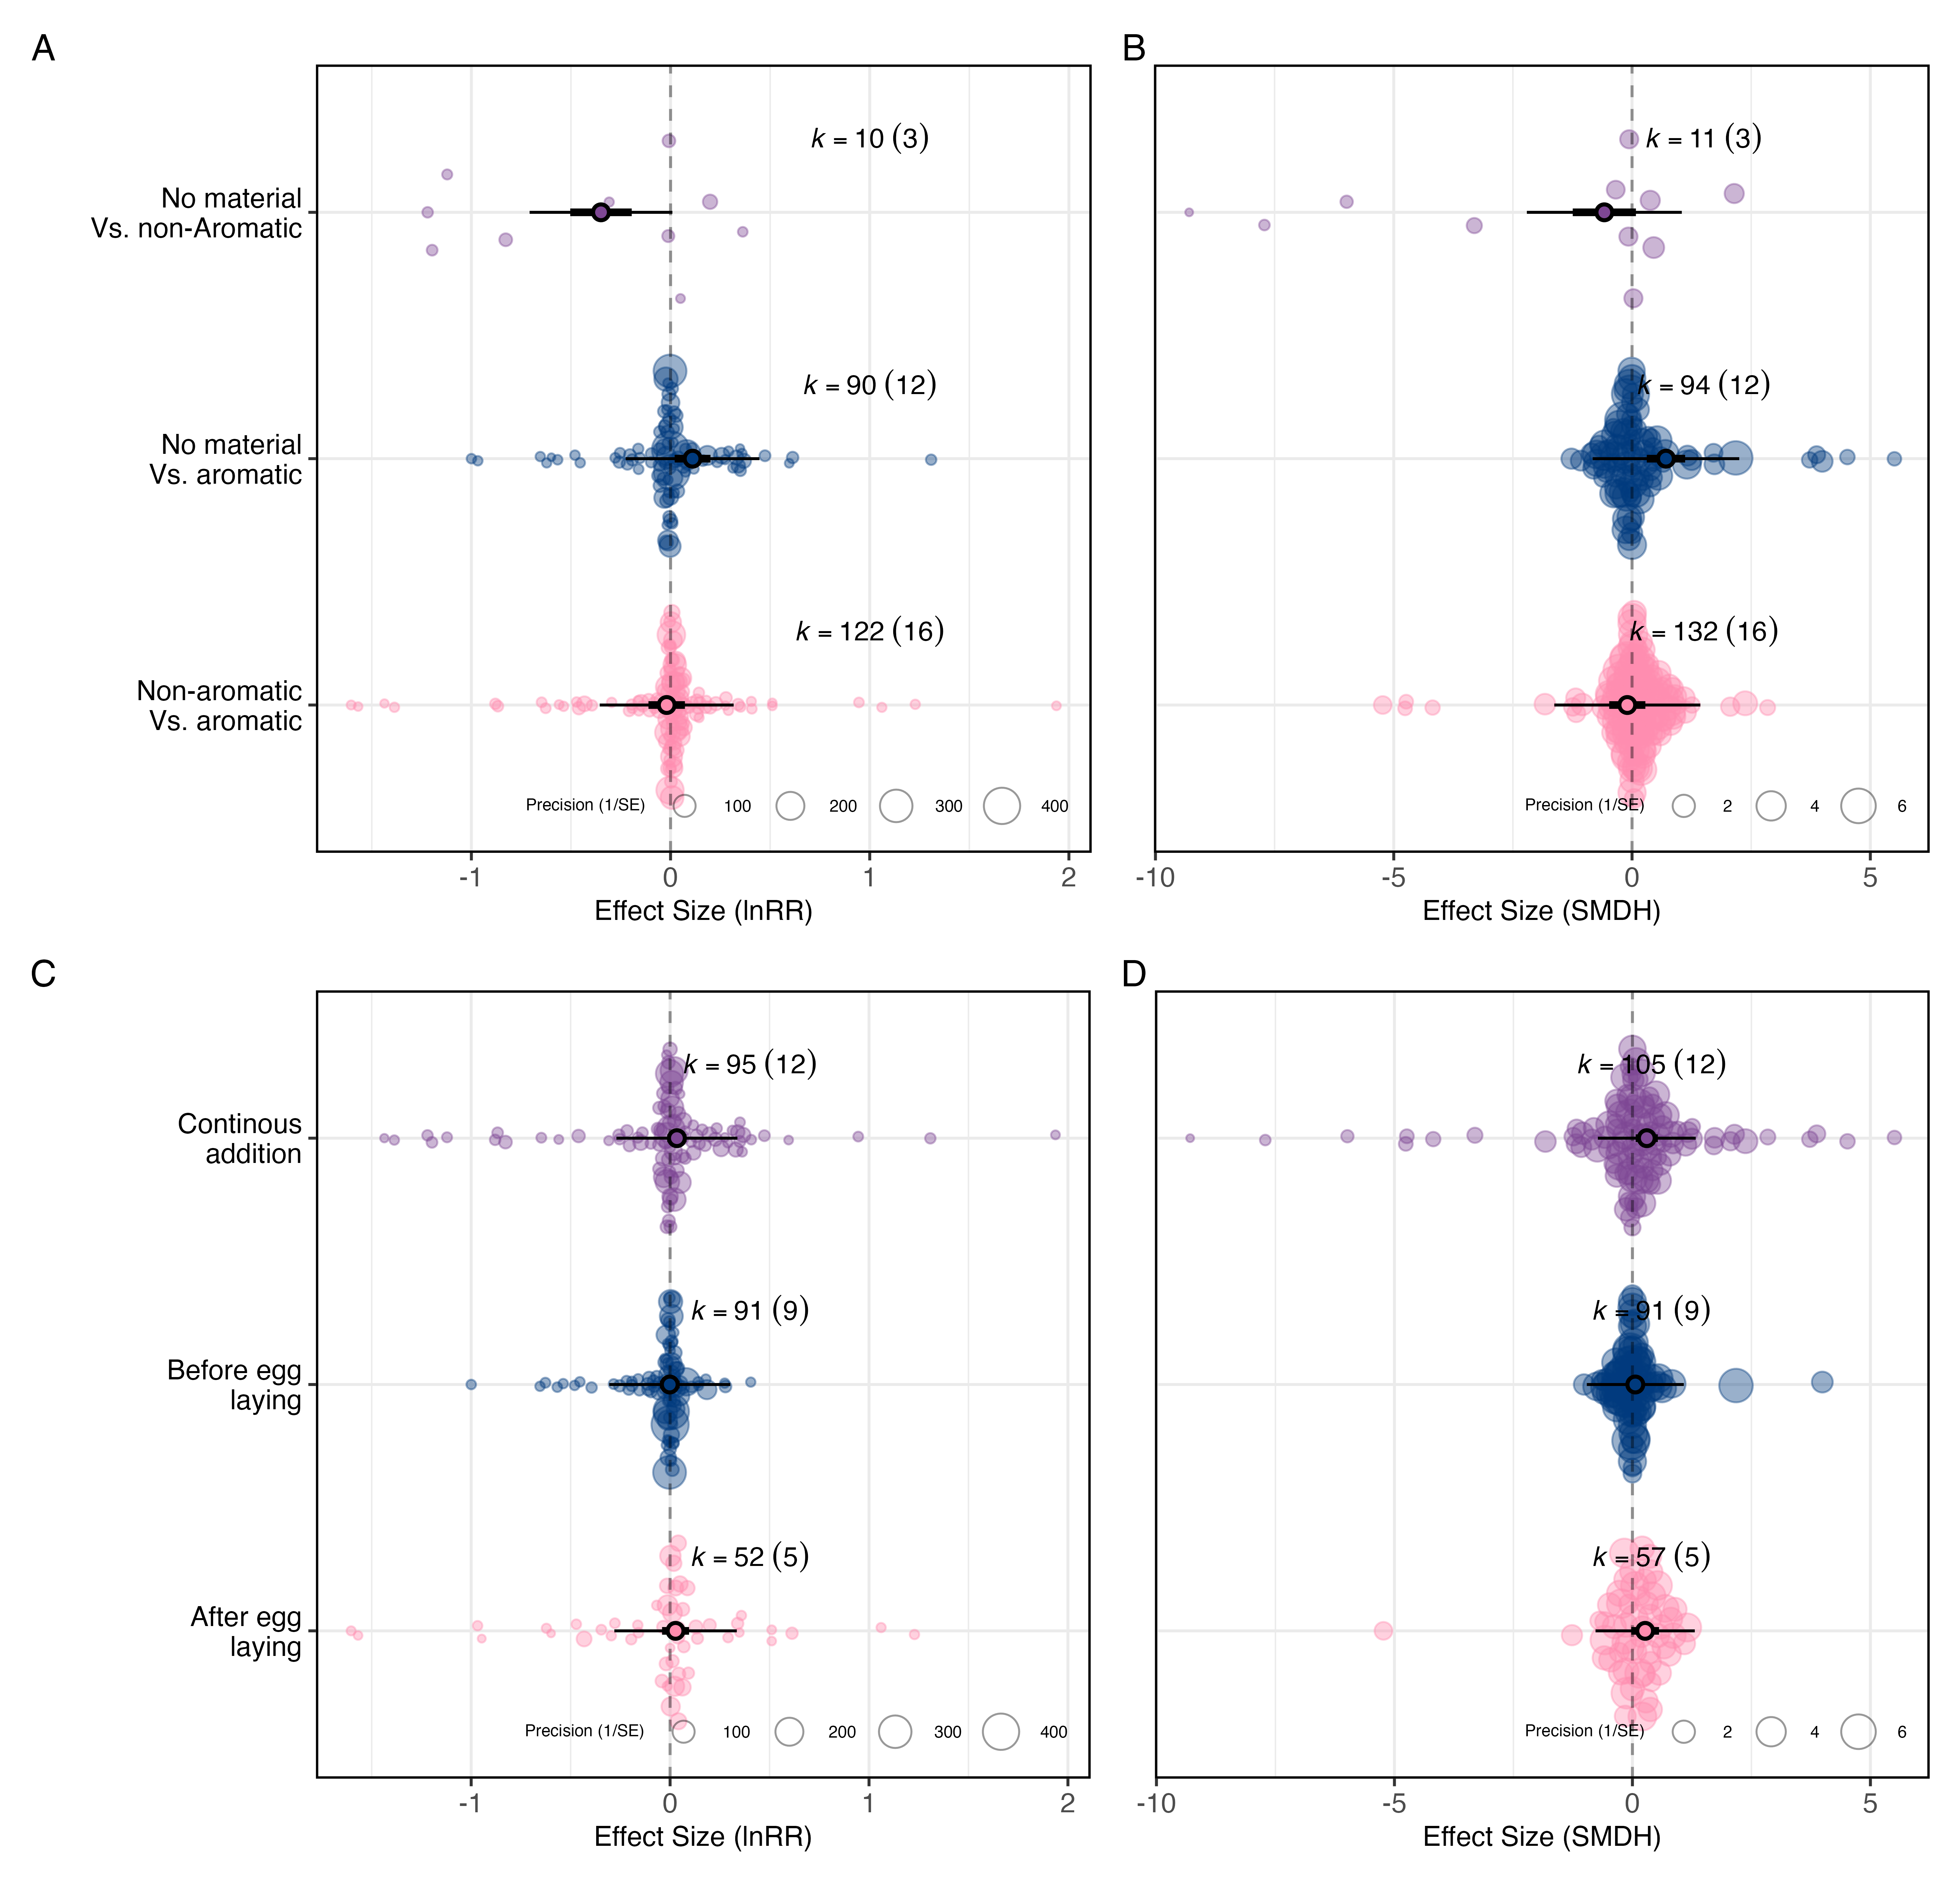
\includegraphics[width=0.9\linewidth,height=\textheight,keepaspectratio]{figures/Figure_design_time_gnm_addition.png}

}

\caption{\label{figsupp-design-time}Experimental designs comparing nests
with aromatic green nest material against nests without any green
material, and those adding the material continuously, lead to the
largest fitness estimates. Orchard plots of the multilevel
meta-regressions showing the overall effect of green nest material
depending on experimental design for (A: log response ratio (lnRR); B:
standardised mean difference (SMD(H)), and time of green nest material
addition (C: log response ratio (lnRR); D: standardised mean difference
(SMD(H)). Mean estimates (black circles), 95\% confidence intervals
(thicker bars) and prediction intervals (thinner bars) are shown along
the individual data points (transparently coloured circles) scaled by
precision (inverse of standard error). k: number of effect sizes (number
of studies is shown in the brackets).}

\end{figsupp}%

\begin{figsupp}

\centering{

\includegraphics[width=0.9\linewidth,height=\textheight,keepaspectratio]{figures/Figure_parasite_birds_trait.png}

}

\caption{\label{figsupp-MR}Orchard plot of the multilevel
meta-regression for (A) log response ratio (lnRR) and (B) standardised
mean difference (SMD(H)). Mean estimates (black circles), 95\%
confidence intervals (thicker bars), and prediction intervals (thinner
bars) are shown along with the individual data points (transparently
coloured circles) scaled by precision (inverse of standard error). k:
number of effect sizes (number of studies is shown in the brackets).}

\end{figsupp}%

\subsection{Risk of Bias Test}\label{risk-of-bias-test}

The risk of bias categories we evaluated (i.e., blinding, random
assignment to each treatment and partial reporting) were not
statistically significant for lnRR (\quartotabsuppref{tabsupp-SA-RoB}).
SMD(H) was positive and statistically significant for studies without
blinding (SMD(H)\textsubscript{No~Blinding} = 0.184, 95\% CI: {[} 0.051,
0.316{]}, 95\% PI: {[}-0.828, 1.195{]}, p-value = 0.007, k = 242, n =
25; \quartotabsuppref{tabsupp-SA-RoB}), with random assignment to
treatment (SMD(H)\textsubscript{Random~Assignment} = 0.205, 95\% CI: {[}
0.049, 0.360{]}, 95\% PI: {[}-0.813, 1.223{]}, p-value = 0.010, k = 225,
n = 23; \quartotabsuppref{tabsupp-SA-RoB}) and where no data was missing
(SMD(H)\textsubscript{No~Partial~Reporting} = 0.196, 95\% CI: {[} 0.055,
0.337{]}, 95\% PI: {[}-0.817, 1.209{]}, p-value = 0.007, k = 216, n =
22; \quartotabsuppref{tabsupp-SA-RoB}). Notably, other levels of each
category included fewer than four studies, indicating that the observed
significance likely reflects the higher statistical power in the larger
sample level rather than any systematic bias. All the three categories
for risk of bias explained very little heterogeneity
(\(R^2_{marginal(lnRR)}\)\textgreater{} 0.8\%;
\(R^2_{marginal(SMD(H))}\)\textgreater{} 0.7\%).

\begin{tabsupp}

\centering{

\pandocbounded{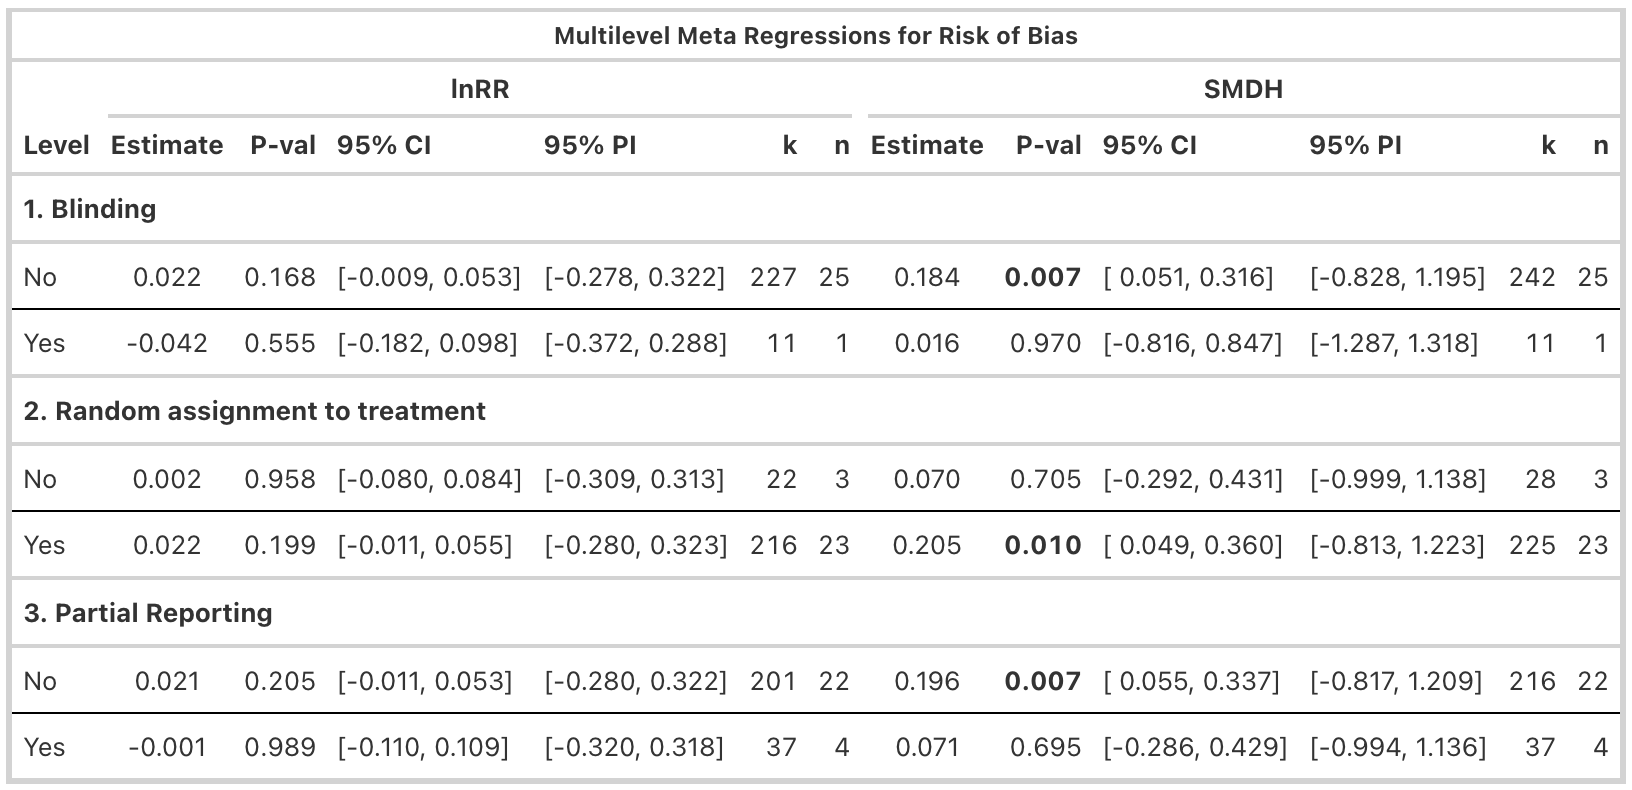
\includegraphics[keepaspectratio]{tables/SA_RoB_table.png}}

}

\caption{\label{tabsupp-SA-RoB}}

\end{tabsupp}%

\subsection{Publication Bias}\label{publication-bias-1}

Since published effect sizes did not seem to change considerably over
time, our analyses suggest no clear evidence of decline effects (i.e.,
time-lag bias) in published effect sizes (lnRR\textsubscript{intercept}
= 0.021, 95\% CI: {[}-0.011; 0.053{]}, p-value = 0.196,
lnRR\textsubscript{slope} = -0.002, 95\% CI: {[}-0.005 to 0.001{]},
p-value = 0.225, k = 221, n = 24, \(R^2_{marginal(lnRR)}\)= 1.8\%;
SMDH\textsubscript{intercept} = 0.193, 95\% CI: {[}0.058 to 0.329{]},
p-value = 0.005, SMDH\textsubscript{slope} = -0.008, 95\% CI: {[}-0.023
to 0.006{]}, p-value = 0.264, k = 235, n = 24,
\(R^2_{marginal(SMD(H))}\) = 2.9\%).

\begin{figsupp}

\centering{

\pandocbounded{\includegraphics[keepaspectratio]{figures/Figure_publication_bias.png}}

}

\caption{\label{figsupp-pub-bias}Tests for publication bias in the
effect of green nest material on fitness outcomes. Plots show
relationships between effect sizes and (A--B) the inverse of effective
sample size (√1/𝑁ₑff) testing for small-study effects, and (C--D)
publication year (mean-centered) testing for time-lag bias, for log
response ratio (lnRR, A and C) and standardized mean difference (SMD(H),
B and D). Points represent individual effect sizes, scaled by precision
(1/SE). Solid lines show meta-regression slopes, with 95\% confidence
intervals (dashed lines) and 95\% prediction intervals (dotted lines).
k: number of effect sizes included in each analysis.}

\end{figsupp}%

\begin{figsupp}

\centering{

\subsection{Systematic Search
Information}\label{systematic-search-information}

}

\caption{\label{figsupp-string}}

\end{figsupp}%

The search was conducted twice, the first time on 07.09.2022 and then
repeated on 12.08.2024 to ensure it was the most up to date and did not
miss any additional articles on the topic that were published meanwhile.
For both the searches, we did not use any time limitation i.e.~it
included all the published literature till that given date. We used
\textbf{Advance Search} option for both Web of Science Core Collection
Database and Scopus Database using the search query given below.\\
\strut \\
Search string for the Web of Science Core Collection\\
Databases used in the search included\\
-Science Citation Index Expanded (SCI-EXPANDED) {[}1900-present{]}\\
-Social Sciences Citation Index (SSCI) {[}1900-present{]}\\
-Arts \& Humanities Citation Index (AHCI) {[}1975 - present{]}\\
-Conference Proceedings Citation Index - Science (CPCI-S) {[}1991 -
present{]}\\
-Conference Proceedings Citation Index - Social Science \& Humanities
(CPCI-SSH) {[}1991 - present{]}\\
-Emerging Sources Citation Index (ESCI) {[}2017- present{]}\\
\strut \\
We used advance search option and Title (TI), Abstract (AB) and Author
Keywords (AK) to conduct our systematic search using the following
string\\
\strut \\
\textless TI=(((``green*'' OR ``herb*'' OR ``aromatic*'') AND ``nest*''
AND (``bird*'' OR ``aves'' OR ``avian'' OR ``ornithol*'' OR
``passerine*'' OR ``passeriform*'' OR ``songbird*'' OR ``Accipiter'' OR
``Aegypius'' OR ``Aquila'' OR ``Aviceda'' OR ``Busarellus'' OR
``Butastur'' OR ``Buteo'' OR ``Buteogallus'' OR ``Chondrohierax'' OR
``Circaetus'' OR ``Circus'' OR ``Clanga'' OR ``Elanoides'' OR ``Elanus''
OR ``Gampsonyx'' OR ``Geranoaetus'' OR ``Geranospiza'' OR ``Gypaetus''
OR ``Gypohierax'' OR ``Gyps'' OR ``Haliaeetus'' OR ``Haliastur'' OR
``Harpagus'' OR ``Harpia'' OR ``Hieraaetus'' OR ``Ictinaetus'' OR
``Ictinia'' OR ``Kaupifalco'' OR ``Leptodon'' OR ``Leucopternis'' OR
``Lophotriorchis'' OR ``Milvus'' OR ``Morphnarchus'' OR ``Morphnus'' OR
``Necrosyrtes'' OR ``Neophron'' OR ``Nisaetus'' OR ``Parabuteo'' OR
``Pernis'' OR ``Pithecophaga'' OR ``Polemaetus'' OR ``Pseudastur'' OR
``Rostrhamus'' OR ``Rupornis'' OR ``Sarcogyps'' OR ``Spilornis'' OR
``Spizaetus'' OR ``Stephanoaetus'' OR ``Terathopius'' OR ``Torgos'' OR
``Trigonoceps'' OR ``Cathartes'' OR ``Coragyps'' OR ``Gymnogyps'' OR
``Sarcoramphus'' OR ``Vultur'' OR ``Pandion'' OR ``Sagittarius'' OR
``Aix'' OR ``Alopochen'' OR ``Amazonetta'' OR ``Anas'' OR ``Anser'' OR
``Asarcornis'' OR ``Aythya'' OR ``Branta'' OR ``Bucephala'' OR
``Cairina'' OR ``Callonetta'' OR ``Cereopsis'' OR ``Chen'' OR
``Chenonetta'' OR ``Chloephaga'' OR ``Clangula'' OR ``Coscoroba'' OR
``Cyanochen'' OR ``Cygnus'' OR''Dendrocygna'' OR ``Heteronetta'' OR
``Histrionicus'' OR ``Hymenolaimus'' OR ``Lophodytes'' OR ``Lophonetta''
OR ``Malacorhynchus'' OR ``Mareca'' OR ``Marmaronetta'' OR ``Melanitta''
OR ``Merganetta'' OR ``Mergellus'' OR ``Mergus'' OR ``Neochen'' OR
``Netta'' OR ``Nettapus'' OR ``Nomonyx'' OR ``Oxyura'' OR
``Plectropterus'' OR ``Polysticta'' OR ``Pteronetta'' OR
``Sarkidiornis'' OR ``Sibirionetta'' OR ``Somateria'' OR ``Spatula'' OR
``Tachyeres'' OR ``Tadorna'' OR ``Thalassornis'' OR ``Anhima'' OR
``Chauna'' OR ``Anseranas'' OR ``Aegotheles'' OR ``Aerodramus'' OR
``Aeronautes'' OR ``Apus'' OR ``Chaetura'' OR ``Collocalia'' OR
``Cypseloides'' OR ``Cypsiurus'' OR ``Hirundapus'' OR ``Panyptila'' OR
``Streptoprocne'' OR ``Tachornis'' OR ``Tachymarptis'' OR ``Hemiprocne''
OR ``Abeillia'' OR ``Adelomyia'' OR ``Aglaeactis'' OR ``Aglaiocercus''
OR ``Amazilia'' OR ``Androdon'' OR ``Anopetia'' OR ``Anthocephala'' OR
``Anthracothorax'' OR ``Archilochus'' OR ``Atthis'' OR ``Augastes'' OR
``Avocettula'' OR ``Basilinna'' OR ``Boissonneaua'' OR ``Calliphlox'' OR
``Calypte'' OR ``Campylopterus'' OR ``Chaetocercus'' OR ``Chalcostigma''
OR ``Chalybura'' OR ``Chlorestes'' OR ``Chlorostilbon'' OR
``Chrysolampis'' OR ``Chrysuronia'' OR ``Clytolaema'' OR ``Coeligena''
OR ``Colibri'' OR ``Cyanophaia'' OR ``Cynanthus'' OR ``Discosura'' OR
``Doricha'' OR ``Doryfera'' OR ``Elvira'' OR ``Ensifera'' OR
``Eriocnemis'' OR ``Eugenes'' OR ``Eulampis'' OR ``Eulidia'' OR
``Eupetomena'' OR ``Eupherusa'' OR ``Eutoxeres'' OR ``Florisuga'' OR
``Glaucis'' OR ``Goethalsia'' OR ``Goldmania'' OR ``Haplophaedia'' OR
``Heliactin'' OR ``Heliangelus'' OR ``Heliodoxa'' OR ``Heliomaster'' OR
``Heliothryx'' OR ``Hylocharis'' OR ``Juliamyia'' OR ``Klais'' OR
``Lafresnaya'' OR ``Lampornis'' OR ``Lamprolaima'' OR ``Lepidopyga'' OR
``Lesbia'' OR ``Leucippus'' OR ``Leucochloris'' OR ``Lophornis'' OR
``Mellisuga'' OR ``Metallura'' OR ``Microchera'' OR ``Myrmia'' OR
``Myrtis'' OR ``Ocreatus'' OR ``Opisthoprora'' OR ``Oreonympha'' OR
``Oreotrochilus'' OR ``Orthorhyncus'' OR ``Oxypogon'' OR ``Panterpe'' OR
``Patagona'' OR ``Phaeochroa'' OR ``Phaethornis'' OR ``Phlogophilus'' OR
``Polyonymus'' OR ``Polytmus'' OR ``Pterophanes'' OR ``Ramphodon'' OR
``Ramphomicron'' OR ``Rhodopis'' OR ``Sappho'' OR ``Schistes'' OR
``Selasphorus'' OR ``Sephanoides'' OR ``Stephanoxis'' OR ``Sternoclyta''
OR ``Taphrospilus'' OR ``Thalurania'' OR ``Thaumastura'' OR
``Threnetes'' OR ``Topaza'' OR ``Trochilus'' OR ``Urochroa'' OR
``Urosticte'' OR ``Apteryx'' OR ``Anthracoceros'' OR ``Buceros'' OR
``Bycanistes'' OR ``Lophoceros'' OR ``Penelopides'' OR
``Rhabdotorrhinus'' OR ``Rhyticeros'' OR ``Tockus'' OR ``Bucorvus'' OR
``Phoeniculus'' OR ``Rhinopomastus'' OR ``Upupa'' OR ``Antrostomus'' OR
``Caprimulgus'' OR ``Chordeiles'' OR ``Eleothreptus'' OR
``Eurostopodus'' OR ``Hydropsalis'' OR ``Lurocalis'' OR ``Lyncornis'' OR
``Nyctidromus'' OR ``Nyctiphrynus'' OR ``Nyctipolus'' OR ``Nyctiprogne''
OR ``Phalaenoptilus'' OR ``Setopagis'' OR ``Systellura'' OR
``Uropsalis'' OR ``Nyctibius'' OR ``Batrachostomus'' OR ``Podargus'' OR
``Steatornis'' OR ``Cariama'' OR ``Casuarius'' OR ``Dromaius'' OR
``Aethia'' OR ``Alca'' OR ``Alle'' OR ``Brachyramphus'' OR ``Cepphus''
OR ``Cerorhinca'' OR ``Fratercula'' OR ``Pinguinus'' OR
``Ptychoramphus'' OR ``Synthliboramphus'' OR ``Uria'' OR ``Burhinus'' OR
``Anarhynchus'' OR ``Charadrius'' OR ``Elseyornis'' OR ``Erythrogonys''
OR ``Hoploxypterus'' OR ``Oreopholus'' OR ``Peltohyas'' OR ``Phegornis''
OR ``Pluvialis'' OR ``Thinornis'' OR ``Vanellus'' OR ``Chionis'' OR
``Dromas'' OR ``Cursorius'' OR ``Glareola'' OR ``Rhinoptilus'' OR
``Stiltia'' OR ``Haematopus'' OR ``Actophilornis'' OR ``Hydrophasianus''
OR ``Irediparra'' OR ``Jacana'' OR ``Metopidius'' OR ``Microparra'' OR
``Anous'' OR ``Chlidonias'' OR ``Chroicocephalus'' OR ``Creagrus'' OR
``Gelochelidon'' OR ``Gygis'' OR ``Hydrocoloeus'' OR ``Hydroprogne'' OR
``Ichthyaetus'' OR ``Larosterna'' OR ``Larus'' OR ``Leucophaeus'' OR
``Onychoprion'' OR ``Pagophila'' OR ``Phaetusa'' OR ``Rhodostethia'' OR
``Rissa'' OR ``Rynchops'' OR ``Sterna'' OR ``Sternula'' OR
``Thalasseus'' OR ``Xema'' OR ``Pedionomus'' OR ``Pluvianellus'' OR
``Pluvianus'' OR ``Himantopus'' OR ``Recurvirostra'' OR ``Nycticryphes''
OR ``Rostratula'' OR ``Actitis'' OR ``Arenaria'' OR ``Bartramia'' OR
``Calidris'' OR ``Coenocorypha'' OR ``Gallinago'' OR ``Limnodromus'' OR
``Limosa'' OR ``Lymnocryptes'' OR ``Numenius'' OR ``Phalaropus'' OR
``Scolopax'' OR ``Tringa'' OR ``Xenus'' OR ``Stercorarius'' OR
``Attagis'' OR ``Thinocorus'' OR ``Turnix'' OR ``Ciconia'' OR
``Ephippiorhynchus'' OR ``Jabiru'' OR ``Leptoptilos'' OR ``Mycteria'' OR
``Colius'' OR ``Urocolius'' OR ``Alectroenas'' OR ``Alopecoenas'' OR
``Caloenas'' OR ``Chalcophaps'' OR ``Claravis'' OR ``Columba'' OR
``Columbina'' OR ``Didunculus'' OR ``Drepanoptila'' OR ``Ducula'' OR
``Ectopistes'' OR ``Gallicolumba'' OR ``Geopelia'' OR ``Geophaps'' OR
``Geotrygon'' OR ``Goura'' OR ``Gymnophaps'' OR ``Hemiphaga'' OR
``Henicophaps'' OR ``Leptotila'' OR ``Leptotrygon'' OR ``Leucosarcia''
OR ``Lopholaimus'' OR ``Macropygia'' OR ``Metriopelia'' OR ``Ocyphaps''
OR ``Oena'' OR ``Otidiphaps'' OR ``Patagioenas'' OR ``Petrophassa'' OR
``Pezophaps'' OR ``Phapitreron'' OR ``Phaps'' OR ``Ptilinopus'' OR
``Raphus'' OR ``Reinwardtoena'' OR ``Spilopelia'' OR ``Streptopelia'' OR
``Treron'' OR ``Trugon'' OR ``Turacoena'' OR ``Turtur'' OR ``Uropelia''
OR ``Zenaida'' OR ``Zentrygon'' OR ``Actenoides'' OR ``Alcedo'' OR
``Caridonax'' OR ``Ceryle'' OR ``Ceyx'' OR ``Chloroceryle'' OR
``Cittura'' OR ``Corythornis'' OR ``Dacelo'' OR ``Halcyon'' OR
``Ispidina'' OR ``Lacedo'' OR ``Megaceryle'' OR ``Melidora'' OR ``Syma''
OR ``Tanysiptera'' OR ``Todiramphus'' OR ``Atelornis'' OR
``Brachypteracias'' OR ``Geobiastes'' OR ``Coracias'' OR ``Eurystomus''
OR ``Merops'' OR ``Nyctyornis'' OR ``Baryphthengus'' OR ``Electron'' OR
``Eumomota'' OR ``Hylomanes'' OR ``Momotus'' OR ``Todus'' OR
``Cacomantis'' OR ``Carpococcyx'' OR ``Centropus'' OR ``Cercococcyx'' OR
``Chrysococcyx'' OR ``Clamator'' OR ``Coccycua'' OR ``Coccyzus'' OR
``Coua'' OR ``Crotophaga'' OR ``Cuculus'' OR ``Dasylophus'' OR
``Dromococcyx'' OR ``Eudynamys'' OR ``Geococcyx'' OR ``Guira'' OR
``Hierococcyx'' OR ``Morococcyx'' OR ``Neomorphus'' OR ``Pachycoccyx''
OR ``Phaenicophaeus'' OR ``Piaya'' OR ``Rhinortha'' OR ``Scythrops'' OR
``Surniculus'' OR ``Tapera'' OR ``Urodynamis'' OR ``Zanclostomus'' OR
``Dinornis'' OR ``Anomalopteryx'' OR ``Emeus'' OR ``Euryapteryx'' OR
``Eurypyga'' OR ``Rhynochetos'' OR ``Caracara'' OR ``Daptrius'' OR
``Falco'' OR ``Herpetotheres'' OR ``Ibycter'' OR ``Micrastur'' OR
``Microhierax'' OR ``Milvago'' OR ``Phalcoboenus'' OR ``Polihierax'' OR
``Spiziapteryx'' OR ``Aburria'' OR ``Chamaepetes'' OR ``Crax'' OR
``Mitu'' OR ``Nothocrax'' OR ``Oreophasis'' OR ``Ortalis'' OR ``Pauxi''
OR ``Penelope'' OR ``Penelopina'' OR ``Pipile'' OR ``Alectura'' OR
``Megapodius'' OR ``Acryllium'' OR ``Guttera'' OR ``Numida'' OR
``Callipepla'' OR ``Colinus'' OR ``Cyrtonyx'' OR ``Dendrortyx'' OR
``Odontophorus'' OR ``Oreortyx'' OR ``Philortyx'' OR ``Ptilopachus'' OR
``Rhynchortyx'' OR ``Alectoris'' OR ``Ammoperdix'' OR ``Arborophila'' OR
``Argusianus'' OR ``Bambusicola'' OR ``Bonasa'' OR ``Caloperdix'' OR
``Centrocercus'' OR ``Chrysolophus'' OR ``Coturnix'' OR ``Crossoptilon''
OR ``Dendragapus'' OR ``Excalfactoria'' OR ``Falcipennis'' OR
``Francolinus'' OR ``Gallus'' OR ``Haematortyx'' OR ``Ithaginis'' OR
``Lagopus'' OR ``Lerwa'' OR ``Lophophorus'' OR ``Lophura'' OR
``Lyrurus'' OR ``Meleagris'' OR ``Pavo'' OR ``Peliperdix'' OR ``Perdix''
OR ``Phasianus'' OR ``Polyplectron'' OR ``Pternistis'' OR ``Pucrasia''
OR ``Rhizothera'' OR ``Rollulus'' OR ``Scleroptila'' OR ``Syrmaticus''
OR ``Tetrao'' OR ``Tetraogallus'' OR ``Tetraophasis'' OR ``Tragopan'' OR
``Tympanuchus'' OR ``Gavia'' OR ``Aramus'' OR ``Anthropoides'' OR
``Antigone'' OR ``Balearica'' OR ``Bugeranus'' OR ``Grus'' OR
``Leucogeranus'' OR ``Heliornis'' OR ``Psophia'' OR ``Aenigmatolimnas''
OR ``Amaurolimnas'' OR ``Amaurornis'' OR ``Anurolimnas'' OR ``Aramides''
OR ``Atlantisia'' OR ``Coturnicops'' OR ``Crex'' OR ``Dryolimnas'' OR
``Eulabeornis'' OR ``Fulica'' OR ``Gallicrex'' OR ``Gallinula'' OR
``Gallirallus'' OR ``Laterallus'' OR ``Lewinia'' OR ``Micropygia'' OR
``Neocrex'' OR ``Nesoclopeus'' OR ``Paragallinula'' OR ``Pardirallus''
OR ``Porphyrio'' OR ``Porphyriops'' OR ``Porzana'' OR ``Rallicula'' OR
``Rallina'' OR ``Rallus'' OR ``Tribonyx'' OR ``Canirallus'' OR
``Sarothrura'' OR ``Leptosomus'' OR ``Corythaeola'' OR
``Corythaixoides'' OR ``Crinifer'' OR ``Musophaga'' OR ``Tauraco'' OR
``Opisthocomus'' OR ``Afrotis'' OR ``Ardeotis'' OR ``Chlamydotis'' OR
``Neotis'' OR ``Otis'' OR ``Tetrax'' OR ``Acanthisitta'' OR
``Pachyplichas'' OR ``Traversia'' OR ``Xenicus'' OR ``Acanthiza'' OR
``Acanthornis'' OR ``Aethomyias'' OR ``Aphelocephala'' OR
``Calamanthus'' OR ``Gerygone'' OR ``Hylacola'' OR ``Neosericornis'' OR
``Oreoscopus'' OR ``Origma'' OR ``Pachycare'' OR ``Pycnoptilus'' OR
``Pyrrholaemus'' OR ``Sericornis'' OR ``Smicrornis'' OR ``Acrocephalus''
OR ``Arundinax'' OR ``Calamonastides'' OR ``Hippolais'' OR ``Iduna'' OR
``Nesillas'' OR ``Aegithalos'' OR ``Leptopoecile'' OR ``Psaltriparus''
OR ``Aegithina'' OR ``Alaemon'' OR ``Alauda'' OR ``Alaudala'' OR
``Ammomanes'' OR ``Calandrella'' OR ``Calendulauda'' OR ``Chersomanes''
OR ``Eremophila'' OR ``Eremopterix'' OR ``Galerida'' OR ``Lullula'' OR
``Melanocorypha'' OR ``Mirafra'' OR ``Pinarocorys'' OR ``Spizocorys'' OR
``Artamus'' OR ``Gymnorhina'' OR ``Melloria'' OR ``Bombycilla'' OR
``Buphagus'' OR ``Calcarius'' OR ``Plectrophenax'' OR ``Rhynchophanes''
OR ``Callaeas'' OR ``Heteralocha'' OR ``Philesturnus'' OR
``Calyptophilus'' OR ``Campephaga'' OR ``Ceblepyris'' OR ``Coracina'' OR
``Edolisoma'' OR ``Lalage'' OR ``Malindangia'' OR ``Pericrocotus'' OR
``Amaurospiza'' OR ``Cardinalis'' OR ``Caryothraustes'' OR
``Chlorothraupis'' OR ``Cyanocompsa'' OR ``Cyanoloxia'' OR
``Granatellus'' OR ``Habia'' OR ``Passerina'' OR ``Periporphyrus'' OR
``Pheucticus'' OR ``Piranga'' OR ``Spiza'' OR ``Certhia'' OR
``Salpornis'' OR ``Abroscopus'' OR ``Cettia'' OR ``Horornis'' OR
``Phyllergates'' OR ``Tesia'' OR ``Urosphena'' OR ``Chloropsis'' OR
``Cinclus'' OR ``Apalis'' OR ``Artisornis'' OR ``Camaroptera'' OR
``Cisticola'' OR ``Eremomela'' OR ``Heliolais'' OR ``Hypergerus'' OR
``Neomixis'' OR ``Oreolais'' OR ``Orthotomus'' OR ``Phragmacia'' OR
``Poliolais'' OR ``Prinia'' OR ``Schistolais'' OR ``Urolais'' OR
``Urorhipis'' OR ``Climacteris'' OR ``Cormobates'' OR ``Conopophaga'' OR
``Struthidea'' OR ``Aphelocoma'' OR ``Calocitta'' OR ``Cissa'' OR
``Coloeus'' OR ``Corvus'' OR ``Cyanocitta'' OR ``Cyanocorax'' OR
``Cyanolyca'' OR ``Cyanopica'' OR ``Dendrocitta'' OR ``Garrulus'' OR
``Gymnorhinus'' OR ``Nucifraga'' OR ``Perisoreus'' OR ``Pica'' OR
``Platylophus'' OR ``Podoces'' OR ``Psilorhinus'' OR ``Ptilostomus'' OR
``Pyrrhocorax'' OR ``Urocissa'' OR ``Ampelioides'' OR ``Ampelion'' OR
``Carpornis'' OR ``Cephalopterus'' OR ``Conioptilon'' OR ``Cotinga'' OR
``Doliornis'' OR ``Gymnoderus'' OR ``Haematoderus'' OR ``Lipaugus'' OR
``Perissocephalus'' OR ``Phoenicircus'' OR ``Phytotoma'' OR ``Pipreola''
OR ``Porphyrolaema'' OR ``Procnias'' OR ``Pyroderus'' OR ``Querula'' OR
``Rupicola'' OR ``Snowornis'' OR ``Xipholena'' OR ``Zaratornis'' OR
``Dasyornis'' OR ``Dicaeum'' OR ``Prionochilus'' OR ``Dicrurus'' OR
``Donacobius'' OR ``Dulus'' OR ``Emberiza'' OR ``Amadina'' OR
``Amandava'' OR ``Cryptospiza'' OR ``Erythrura'' OR ``Estrilda'' OR
``Euodice'' OR ``Euschistospiza'' OR ``Lagonosticta'' OR ``Lonchura'' OR
``Mandingoa'' OR ``Neochmia'' OR ``Nesocharis'' OR ``Nigrita'' OR
``Ortygospiza'' OR ``Parmoptila'' OR ``Pyrenestes'' OR ``Pytilia'' OR
``Spermophaga'' OR ``Stagonopleura'' OR ``Taeniopygia'' OR
``Uraeginthus'' OR ``Calyptomena'' OR ``Cymbirhynchus'' OR
``Eurylaimus'' OR ``Psarisomus'' OR ``Serilophus'' OR ``Smithornis'' OR
``Chamaeza'' OR ``Formicarius'' OR ``Acanthis'' OR ``Agraphospiza'' OR
``Akialoa'' OR ``Bucanetes'' OR ``Carduelis'' OR ``Carpodacus'' OR
``Chloris'' OR ``Chlorodrepanis'' OR ``Chlorophonia'' OR
``Chrysocorythus'' OR ``Coccothraustes'' OR ``Crithagra'' OR
``Drepanis'' OR ``Eophona'' OR ``Euphonia'' OR ``Fringilla'' OR
``Haemorhous'' OR ``Hemignathus'' OR ``Himatione'' OR ``Leucosticte'' OR
``Linaria'' OR ``Linurgus'' OR ``Loxia'' OR ``Loxioides'' OR ``Loxops''
OR ``Magumma'' OR ``Melamprosops'' OR ``Oreomystis'' OR ``Paroreomyza''
OR ``Pinicola'' OR ``Procarduelis'' OR ``Pseudonestor'' OR
``Psittirostra'' OR ``Pyrrhoplectes'' OR ``Pyrrhula'' OR ``Rhodopechys''
OR ``Rhodospiza'' OR ``Serinus'' OR ``Spinus'' OR ``Telespiza'' OR
``Anabacerthia'' OR ``Anabazenops'' OR ``Ancistrops'' OR ``Anumbius'' OR
``Aphrastura'' OR ``Asthenes'' OR ``Automolus'' OR ``Berlepschia'' OR
``Campylorhamphus'' OR ``Certhiasomus'' OR ``Certhiaxis'' OR
``Cinclodes'' OR ``Clibanornis'' OR ``Coryphistera'' OR ``Cranioleuca''
OR ``Deconychura'' OR ``Dendrexetastes'' OR ``Dendrocincla'' OR
``Dendrocolaptes'' OR ``Dendroplex'' OR ``Drymornis'' OR
``Drymotoxeres'' OR ``Furnarius'' OR ``Geocerthia'' OR ``Geositta'' OR
``Glyphorynchus'' OR ``Heliobletus'' OR ``Hellmayrea'' OR
``Hylexetastes'' OR ``Lepidocolaptes'' OR ``Leptasthenura'' OR
``Limnoctites'' OR ``Limnornis'' OR ``Lochmias'' OR ``Margarornis'' OR
``Mazaria'' OR ``Megaxenops'' OR ``Metopothrix'' OR ``Microxenops'' OR
``Nasica'' OR ``Ochetorhynchus'' OR ``Phacellodomus'' OR ``Philydor'' OR
``Phleocryptes'' OR ``Premnoplex'' OR ``Premnornis'' OR
``Pseudasthenes'' OR ``Pseudocolaptes'' OR ``Pseudoseisura'' OR
``Pygarrhichas'' OR ``Roraimia'' OR ``Schoeniophylax'' OR ``Sclerurus''
OR ``Sittasomus'' OR ``Spartonoica'' OR ``Sylviorthorhynchus'' OR
``Synallaxis'' OR ``Syndactyla'' OR ``Tarphonomus'' OR ``Thripadectes''
OR ``Thripophaga'' OR ``Upucerthia'' OR ``Xenerpestes'' OR ``Xenops'' OR
``Xiphocolaptes'' OR ``Xiphorhynchus'' OR ``Grallaria'' OR
``Grallaricula'' OR ``Hylopezus'' OR ``Myrmothera'' OR ``Alopochelidon''
OR ``Atticora'' OR ``Cecropis'' OR ``Delichon'' OR ``Haplochelidon'' OR
``Hirundo'' OR ``Neochelidon'' OR ``Notiochelidon'' OR ``Orochelidon''
OR ``Petrochelidon'' OR ``Phedina'' OR ``Progne'' OR ``Psalidoprocne''
OR ``Pseudhirundo'' OR ``Pseudochelidon'' OR ``Ptyonoprogne'' OR
``Riparia'' OR ``Stelgidopteryx'' OR ``Tachycineta'' OR ``Hyliota'' OR
``Hypocolius'' OR ``Agelaioides'' OR ``Agelaius'' OR ``Agelasticus'' OR
``Amblycercus'' OR ``Amblyramphus'' OR ``Anumara'' OR ``Cacicus'' OR
``Chrysomus'' OR ``Curaeus'' OR ``Dives'' OR ``Dolichonyx'' OR
``Euphagus'' OR ``Gnorimopsar'' OR ``Gymnomystax'' OR ``Hypopyrrhus'' OR
``Icterus'' OR ``Lampropsar'' OR ``Leistes'' OR ``Macroagelaius'' OR
``Molothrus'' OR ``Nesopsar'' OR ``Oreopsar'' OR ``Psarocolius'' OR
``Pseudoleistes'' OR ``Quiscalus'' OR ``Sturnella'' OR
``Xanthocephalus'' OR ``Xanthopsar'' OR ``Icteria'' OR ``Ifrita'' OR
``Irena'' OR ``Corvinella'' OR ``Eurocephalus'' OR ``Lanius'' OR
``Actinodura'' OR ``Argya'' OR ``Garrulax'' OR ``Grammatoptila'' OR
``Heterophasia'' OR ``Ianthocincla'' OR ``Laniellus'' OR ``Leiothrix''
OR ``Liocichla'' OR ``Minla'' OR ``Pterorhinus'' OR ``Trochalopteron''
OR ``Turdoides'' OR ``Bradypterus'' OR ``Cincloramphus'' OR
``Helopsaltes'' OR ``Locustella'' OR ``Megalurus'' OR ``Poodytes'' OR
``Machaerirhynchus'' OR ``Graueria'' OR ``Hylia'' OR ``Macrosphenus'' OR
``Melocichla'' OR ``Sylvietta'' OR ``Chlorophoneus'' OR ``Dryoscopus''
OR ``Laniarius'' OR ``Malaconotus'' OR ``Nilaus'' OR ``Rhodophoneus'' OR
``Tchagra'' OR ``Telophorus'' OR ``Amytornis'' OR ``Chenorhamphus'' OR
``Clytomyias'' OR ``Malurus'' OR ``Stipiturus'' OR ``Melampitta'' OR
``Melanocharis'' OR ``Oedistoma'' OR ``Toxorhamphus'' OR
``Melanopareia'' OR ``Acanthagenys'' OR ``Acanthorhynchus'' OR
``Anthochaera'' OR ``Anthornis'' OR ``Caligavis'' OR ``Entomyzon'' OR
``Epthianura'' OR ``Glycifohia'' OR ``Gymnomyza'' OR ``Lichmera'' OR
``Manorina'' OR ``Melidectes'' OR ``Melilestes'' OR ``Meliphaga'' OR
``Melipotes'' OR ``Melithreptus'' OR ``Myzomela'' OR ``Nesoptilotis'' OR
``Philemon'' OR ``Phylidonyris'' OR ``Prosthemadera'' OR ``Ptiloprora''
OR ``Ptilotula'' OR ``Pycnopygius'' OR ``Timeliopsis'' OR ``Xanthotis''
OR ``Menura'' OR ``Allenia'' OR ``Cinclocerthia'' OR ``Dumetella'' OR
``Margarops'' OR ``Melanoptila'' OR ``Melanotis'' OR ``Mimus'' OR
``Oreoscoptes'' OR ``Ramphocinclus'' OR ``Toxostoma'' OR ``Lamprospiza''
OR ``Mitrospingus'' OR ``Moho'' OR ``Mohoua'' OR ``Arses'' OR
``Carterornis'' OR ``Clytorhynchus'' OR ``Grallina'' OR ``Hypothymis''
OR ``Monarcha'' OR ``Myiagra'' OR ``Symposiachrus'' OR ``Terpsiphone''
OR ``Trochocercus'' OR ``Anthus'' OR ``Macronyx'' OR ``Motacilla'' OR
``Alethe'' OR ``Anthipes'' OR ``Brachypteryx'' OR ``Calliope'' OR
``Campicoloides'' OR ``Cercotrichas'' OR ``Chamaetylas'' OR
``Copsychus'' OR ``Cossypha'' OR ``Cyanoptila'' OR ``Cyornis'' OR
``Enicurus'' OR ``Erithacus'' OR ``Eumyias'' OR ``Ficedula'' OR
``Fraseria'' OR ``Irania'' OR ``Larvivora'' OR ``Leonardina'' OR
``Luscinia'' OR ``Melaenornis'' OR ``Monticola'' OR ``Muscicapa'' OR
``Myiomela'' OR ``Myioparus'' OR ``Myophonus'' OR ``Myrmecocichla'' OR
``Niltava'' OR ``Oenanthe'' OR ``Phoenicurus'' OR ``Pogonocichla'' OR
``Saxicola'' OR ``Sheppardia'' OR ``Sholicola'' OR ``Stiphrornis'' OR
``Tarsiger'' OR ``Thamnolaea'' OR ``Vauriella'' OR ``Aethopyga'' OR
``Anabathmis'' OR ``Anthreptes'' OR ``Arachnothera'' OR ``Chalcomitra''
OR ``Cinnyris'' OR ``Cyanomitra'' OR ``Deleornis'' OR ``Hedydipna'' OR
``Kurochkinegramma'' OR ``Leptocoma'' OR ``Nectarinia'' OR
``Daphoenositta'' OR ``Nesospingus'' OR ``Nicator'' OR ``Notiomystis''
OR ``Aleadryas'' OR ``Oriolus'' OR ``Pitohui'' OR ``Sphecotheres'' OR
``Turnagra'' OR ``Colluricincla'' OR ``Falcunculus'' OR ``Melanorectes''
OR ``Pachycephala'' OR ``Pseudorectes'' OR ``Panurus'' OR ``Cicinnurus''
OR ``Diphyllodes'' OR ``Manucodia'' OR ``Paradisaea'' OR ``Ptiloris'' OR
``Paramythia'' OR ``Pardalotus'' OR ``Baeolophus'' OR ``Cephalopyrus''
OR ``Cyanistes'' OR ``Lophophanes'' OR ``Machlolophus'' OR
``Melaniparus'' OR ``Melanochlora'' OR ``Pardaliparus'' OR ``Parus'' OR
``Periparus'' OR ``Poecile'' OR ``Pseudopodoces'' OR ``Sittiparus'' OR
``Sylviparus'' OR ``Basileuterus'' OR ``Cardellina'' OR ``Catharopeza''
OR ``Dendroica'' OR ``Geothlypis'' OR ``Helmitheros'' OR ``Leiothlypis''
OR ``Limnothlypis'' OR ``Mniotilta'' OR ``Myioborus'' OR ``Myiothlypis''
OR ``Oporornis'' OR ``Oreothlypis'' OR ``Parkesia'' OR ``Protonotaria''
OR ``Seiurus'' OR ``Setophaga'' OR ``Vermivora'' OR ``Aimophila'' OR
``Ammodramus'' OR ``Amphispiza'' OR ``Arremon'' OR ``Arremonops'' OR
``Artemisiospiza'' OR ``Atlapetes'' OR ``Calamospiza'' OR
``Chlorospingus'' OR ``Chondestes'' OR ``Junco'' OR ``Melospiza'' OR
``Melozone'' OR ``Oreothraupis'' OR ``Oriturus'' OR ``Passerculus'' OR
``Passerella'' OR ``Peucaea'' OR ``Pezopetes'' OR ``Pipilo'' OR
``Pooecetes'' OR ``Pselliophorus'' OR ``Rhynchospiza'' OR ``Spizella''
OR ``Spizelloides'' OR ``Xenospiza'' OR ``Zonotrichia'' OR
``Carpospiza'' OR ``Gymnoris'' OR ``Hypocryptadius'' OR
``Montifringilla'' OR ``Onychostruthus'' OR ``Passer'' OR ``Petronia''
OR ``Pyrgilauda'' OR ``Alcippe'' OR ``Gampsorhynchus'' OR ``Illadopsis''
OR ``Jabouilleia'' OR ``Kenopia'' OR ``Laticilla'' OR ``Malacocincla''
OR ``Malacopteron'' OR ``Napothera'' OR ``Pellorneum'' OR ``Rimator'' OR
``Trichastoma'' OR ``Amalocichla'' OR ``Drymodes'' OR ``Eopsaltria'' OR
``Eugerygone'' OR ``Heteromyias'' OR ``Melanodryas'' OR ``Microeca'' OR
``Monachella'' OR ``Pachycephalopsis'' OR ``Peneoenanthe'' OR
``Peneothello'' OR ``Petroica'' OR ``Poecilodryas'' OR ``Tregellasia''
OR ``Peucedramus'' OR ``Microligea'' OR ``Phaenicophilus'' OR
``Xenoligea'' OR ``Phylloscopus'' OR ``Picathartes'' OR ``Antilophia''
OR ``Ceratopipra'' OR ``Chiroxiphia'' OR ``Chloropipo'' OR ``Corapipo''
OR ``Cryptopipo'' OR ``Heterocercus'' OR ``Ilicura'' OR ``Lepidothrix''
OR ``Machaeropterus'' OR ``Manacus'' OR ``Masius'' OR ``Neopelma'' OR
``Pipra'' OR ``Pseudopipra'' OR ``Tyranneutes'' OR ``Xenopipo'' OR
``Erythropitta'' OR ``Hydrornis'' OR ``Pitta'' OR ``Batis'' OR
``Platysteira'' OR ``Anaplectes'' OR ``Bubalornis'' OR ``Euplectes'' OR
``Malimbus'' OR ``Plocepasser'' OR ``Ploceus'' OR ``Quelea'' OR
``Sporopipes'' OR ``Pnoepyga'' OR ``Microbates'' OR ``Polioptila'' OR
``Ramphocaenus'' OR ``Garritornis'' OR ``Prunella'' OR ``Cinclosoma'' OR
``Ptilorrhoa'' OR ``Phainopepla'' OR ``Phainoptila'' OR ``Ptiliogonys''
OR ``Ailuroedus'' OR ``Amblyornis'' OR ``Ptilonorhynchus'' OR
``Sericulus'' OR ``Alophoixus'' OR ``Andropadus'' OR ``Arizelocichla''
OR ``Atimastillas'' OR ``Baeopogon'' OR ``Bleda'' OR ``Chlorocichla'' OR
``Criniger'' OR ``Eurillas'' OR ``Hemixos'' OR ``Hypsipetes'' OR
``Iole'' OR ``Ixos'' OR ``Neolestes'' OR ``Phyllastrephus'' OR
``Pycnonotus'' OR ``Spizixos'' OR ``Stelgidillas'' OR ``Tricholestes''
OR ``Regulus'' OR ``Anthoscopus'' OR ``Auriparus'' OR ``Remiz'' OR
``Rhagologus'' OR ``Eleoscytalopus'' OR ``Liosceles'' OR
``Psilorhamphus'' OR ``Pteroptochos'' OR ``Scelorchilus'' OR
``Scytalopus'' OR ``Teledromas'' OR ``Rhipidura'' OR ``Rhodinocichla''
OR ``Sapayoa'' OR ``Sitta'' OR ``Spindalis'' OR ``Chelidorhynx'' OR
``Culicicapa'' OR ``Elminia'' OR ``Acridotheres'' OR ``Agropsar'' OR
``Ampeliceps'' OR ``Aplonis'' OR ``Basilornis'' OR ``Cinnyricinclus'' OR
``Creatophora'' OR ``Gracula'' OR ``Gracupica'' OR ``Hartlaubius'' OR
``Hylopsar'' OR ``Lamprotornis'' OR ``Leucopsar'' OR ``Mino'' OR
``Notopholia'' OR ``Onychognathus'' OR ``Pastor'' OR ``Poeoptera'' OR
``Rhabdornis'' OR ``Sarcops'' OR ``Scissirostrum'' OR ``Speculipastor''
OR ``Spodiopsar'' OR ``Streptocitta'' OR ``Sturnia'' OR ``Sturnus'' OR
``Chamaea'' OR ``Chleuasicus'' OR ``Chloropeta'' OR ``Chrysomma'' OR
``Conostoma'' OR ``Fulvetta'' OR ``Lioparus'' OR ``Paradoxornis'' OR
``Pseudoalcippe'' OR ``Psittiparus'' OR ``Rhopophilus'' OR
``Sinosuthora'' OR ``Suthora'' OR ``Sylvia'' OR ``Teretistris'' OR
``Akletos'' OR ``Ampelornis'' OR ``Aprositornis'' OR ``Batara'' OR
``Cercomacra'' OR ``Cercomacroides'' OR ``Cymbilaimus'' OR
``Dichrozona'' OR ``Drymophila'' OR ``Dysithamnus'' OR
``Epinecrophylla'' OR ``Euchrepomis'' OR ``Formicivora'' OR
``Frederickena'' OR ``Gymnocichla'' OR ``Gymnopithys'' OR ``Hafferia''
OR ``Herpsilochmus'' OR ``Hylophylax'' OR ``Hypocnemis'' OR
``Hypocnemoides'' OR ``Hypoedaleus'' OR ``Isleria'' OR ``Mackenziaena''
OR ``Megastictus'' OR ``Microrhopias'' OR ``Myrmeciza'' OR
``Myrmelastes'' OR ``Myrmoborus'' OR ``Myrmochanes'' OR ``Myrmoderus''
OR ``Myrmophylax'' OR ``Myrmorchilus'' OR ``Myrmornis'' OR
``Myrmotherula'' OR ``Neoctantes'' OR ``Oneillornis'' OR ``Percnostola''
OR ``Phaenostictus'' OR ``Phlegopsis'' OR ``Pithys'' OR ``Poliocrania''
OR ``Pygiptila'' OR ``Pyriglena'' OR ``Rhegmatorhina'' OR ``Rhopias'' OR
``Rhopornis'' OR ``Sakesphorus'' OR ``Sciaphylax'' OR ``Sclateria'' OR
``Sipia'' OR ``Taraba'' OR ``Thamnistes'' OR ``Thamnomanes'' OR
``Thamnophilus'' OR ``Willisornis'' OR ``Xenornis'' OR ``Anisognathus''
OR ``Bangsia'' OR ``Buthraupis'' OR ``Calochaetes'' OR
``Catamblyrhynchus'' OR ``Catamenia'' OR ``Charitospiza'' OR
``Chlorochrysa'' OR ``Chlorophanes'' OR ``Chlorornis'' OR
``Chrysothlypis'' OR ``Cissopis'' OR ``Cnemoscopus'' OR ``Coereba'' OR
``Compsospiza'' OR ``Compsothraupis'' OR ``Conirostrum'' OR
``Conothraupis'' OR ``Coryphospingus'' OR ``Creurgops'' OR ``Cyanerpes''
OR ``Cyanicterus'' OR ``Cypsnagra'' OR ``Dacnis'' OR ``Delothraupis'' OR
``Diglossa'' OR ``Diuca'' OR ``Dolospingus'' OR ``Donacospiza'' OR
``Dubusia'' OR ``Emberizoides'' OR ``Embernagra'' OR ``Eucometis'' OR
``Euneornis'' OR ``Geospiza'' OR ``Gubernatrix'' OR ``Haplospiza'' OR
``Hemispingus'' OR ``Hemithraupis'' OR ``Heterospingus'' OR
``Incaspiza'' OR ``Iridophanes'' OR ``Iridosornis'' OR ``Lanio'' OR
``Lophospingus'' OR ``Loxigilla'' OR ``Loxipasser'' OR ``Melanodera'' OR
``Melanospiza'' OR ``Melopyrrha'' OR ``Nemosia'' OR ``Nephelornis'' OR
``Oreomanes'' OR ``Oryzoborus'' OR ``Parkerthraustes'' OR ``Paroaria''
OR ``Phrygilus'' OR ``Piezorina'' OR ``Pipraeidea'' OR ``Poospiza'' OR
``Pyrrhocoma'' OR ``Ramphocelus'' OR ``Rhodospingus'' OR ``Saltator'' OR
``Saltatricula'' OR ``Schistochlamys'' OR ``Sericossypha'' OR
``Sicalis'' OR ``Sporophila'' OR ``Stephanophorus'' OR ``Tachyphonus''
OR ``Tangara'' OR ``Tersina'' OR ``Thlypopsis'' OR ``Thraupis'' OR
``Tiaris'' OR ``Trichothraupis'' OR ``Volatinia'' OR ``Wetmorethraupis''
OR ``Xenodacnis'' OR ``Xenospingus'' OR ``Tichodroma'' OR ``Macronus''
OR ``Pomatorhinus'' OR ``Spelaeornis'' OR ``Stachyridopsis'' OR
``Stachyris'' OR ``Iodopleura'' OR ``Laniisoma'' OR ``Laniocera'' OR
``Myiobius'' OR ``Onychorhynchus'' OR ``Oxyruncus'' OR ``Pachyramphus''
OR ``Schiffornis'' OR ``Terenotriccus'' OR ``Tityra'' OR ``Xenopsaris''
OR ``Campylorhynchus'' OR ``Cantorchilus'' OR ``Catherpes'' OR
``Cinnycerthia'' OR ``Cistothorus'' OR ``Cyphorhinus'' OR
``Henicorhina'' OR ``Microcerculus'' OR ``Odontorchilus'' OR
``Pheugopedius'' OR ``Salpinctes'' OR ``Thryomanes'' OR ``Thryophilus''
OR ``Thryothorus'' OR ``Troglodytes'' OR ``Uropsila'' OR ``Catharus'' OR
``Cichlopsis'' OR ``Entomodestes'' OR ``Geokichla'' OR ``Hylocichla'' OR
``Ixoreus'' OR ``Myadestes'' OR ``Neocossyphus'' OR ``Ridgwayia'' OR
``Sialia'' OR ``Stizorhina'' OR ``Turdus'' OR ``Zoothera'' OR
``Agriornis'' OR ``Alectrurus'' OR ``Anairetes'' OR ``Aphanotriccus'' OR
``Arundinicola'' OR ``Atalotriccus'' OR ``Attila'' OR ``Camptostoma'' OR
``Capsiempis'' OR ``Casiornis'' OR ``Cnemarchus'' OR ``Cnemotriccus'' OR
``Cnipodectes'' OR ``Colonia'' OR ``Colorhamphus'' OR ``Conopias'' OR
``Contopus'' OR ``Corythopis'' OR ``Culicivora'' OR ``Deltarhynchus'' OR
``Elaenia'' OR ``Empidonax'' OR ``Empidonomus'' OR ``Euscarthmus'' OR
``Fluvicola'' OR ``Griseotyrannus'' OR ``Gubernetes'' OR ``Hemitriccus''
OR ``Heteroxolmis'' OR ``Hirundinea'' OR ``Hymenops'' OR ``Inezia'' OR
``Knipolegus'' OR ``Lathrotriccus'' OR ``Legatus'' OR ``Leptopogon'' OR
``Lessonia'' OR ``Lophotriccus'' OR ``Machetornis'' OR ``Mecocerculus''
OR ``Megarynchus'' OR ``Mionectes'' OR ``Mitrephanes'' OR
``Muscigralla'' OR ``Muscisaxicola'' OR ``Myiarchus'' OR
``Myiodynastes'' OR ``Myiopagis'' OR ``Myiophobus'' OR ``Myiornis'' OR
``Myiotheretes'' OR ``Myiotriccus'' OR ``Myiozetetes'' OR ``Neopipo'' OR
``Neoxolmis'' OR ``Nephelomyias'' OR ``Ochthoeca'' OR ``Ochthornis'' OR
``Oncostoma'' OR ``Ornithion'' OR ``Phaeomyias'' OR ``Philohydor'' OR
``Phyllomyias'' OR ``Phylloscartes'' OR ``Piprites'' OR ``Pitangus'' OR
``Platyrinchus'' OR ``Poecilotriccus'' OR ``Pogonotriccus'' OR
``Polioxolmis'' OR ``Polystictus'' OR ``Pseudelaenia'' OR
``Pseudocolopteryx'' OR ``Pseudotriccus'' OR ``Pyrocephalus'' OR
``Pyrrhomyias'' OR ``Ramphotrigon'' OR ``Rhynchocyclus'' OR
``Rhytipterna'' OR ``Satrapa'' OR ``Sayornis'' OR ``Serpophaga'' OR
``Silvicultrix'' OR ``Sirystes'' OR ``Stigmatura'' OR ``Sublegatus'' OR
``Suiriri'' OR ``Tachuris'' OR ``Taeniotriccus'' OR ``Todirostrum'' OR
``Tolmomyias'' OR ``Tumbezia'' OR ``Tyrannopsis'' OR ``Tyrannulus'' OR
``Tyrannus'' OR ``Uromyias'' OR ``Xenotriccus'' OR ``Xolmis'' OR
``Zimmerius'' OR ``Urocynchramus'' OR ``Artamella'' OR ``Calicalicus''
OR ``Cyanolanius'' OR ``Euryceros'' OR ``Falculea'' OR ``Hypositta'' OR
``Leptopterus'' OR ``Mystacornis'' OR ``Newtonia'' OR ``Oriolia'' OR
``Philentoma'' OR ``Prionops'' OR ``Pseudobias'' OR ``Schetba'' OR
``Tephrodornis'' OR ``Tylas'' OR ``Vanga'' OR ``Xenopirostris'' OR
``Anomalospiza'' OR ``Vidua'' OR ``Cyclarhis'' OR ``Erpornis'' OR
``Hylophilus'' OR ``Pteruthius'' OR ``Vireo'' OR ``Vireolanius'' OR
``Zeledonia'' OR ``Apalopteron'' OR ``Dasycrotapha'' OR ``Heleia'' OR
``Lophozosterops'' OR ``Sterrhoptilus'' OR ``Yuhina'' OR ``Zosterops''
OR ``Zosterornis'' OR ``Agamia'' OR ``Ardea'' OR ``Ardeola'' OR
``Botaurus'' OR ``Bubulcus'' OR ``Butorides'' OR ``Cochlearius'' OR
``Dupetor'' OR ``Egretta'' OR ``Gorsachius'' OR ``Ixobrychus'' OR
``Nyctanassa'' OR ``Nycticorax'' OR ``Pilherodius'' OR ``Syrigma'' OR
``Tigriornis'' OR ``Tigrisoma'' OR ``Zebrilus'' OR ``Balaeniceps'' OR
``Pelecanus'' OR ``Scopus'' OR ``Bostrychia'' OR ``Eudocimus'' OR
``Geronticus'' OR ``Lophotibis'' OR ``Mesembrinibis'' OR ``Nipponia'' OR
``Phimosus'' OR ``Platalea'' OR ``Plegadis'' OR ``Pseudibis'' OR
``Theristicus'' OR ``Threskiornis'' OR ``Phaethon'' OR ``Phoeniconaias''
OR ``Phoenicoparrus'' OR ``Phoenicopterus'' OR ``Bucco'' OR
``Chelidoptera'' OR ``Hapaloptila'' OR ``Hypnelus'' OR ``Malacoptila''
OR ``Micromonacha'' OR ``Monasa'' OR ``Nonnula'' OR ``Notharchus'' OR
``Nystalus'' OR ``Capito'' OR ``Eubucco'' OR ``Brachygalba'' OR
``Galbalcyrhynchus'' OR ``Galbula'' OR ``Jacamaralcyon'' OR
``Jacamerops'' OR ``Indicator'' OR ``Melichneutes'' OR ``Melignomon'' OR
``Prodotiscus'' OR ``Buccanodon'' OR ``Gymnobucco'' OR ``Lybius'' OR
``Pogoniulus'' OR ``Stactolaema'' OR ``Trachyphonus'' OR ``Psilopogon''
OR ``Blythipicus'' OR ``Campephilus'' OR ``Campethera'' OR ``Celeus'' OR
``Chloropicus'' OR ``Chrysocolaptes'' OR ``Chrysophlegma'' OR
``Colaptes'' OR ``Dendrocopos'' OR ``Dendrocoptes'' OR ``Dendropicos''
OR ``Dinopium'' OR ``Dryobates'' OR ``Dryocopus'' OR ``Gecinulus'' OR
``Geocolaptes'' OR ``Jynx'' OR ``Leiopicus'' OR ``Leuconotopicus'' OR
``Meiglyptes'' OR ``Melanerpes'' OR ``Micropternus'' OR ``Mulleripicus''
OR ``Nesoctites'' OR ``Picoides'' OR ``Piculus'' OR ``Picumnus'' OR
``Picus'' OR ``Reinwardtipicus'' OR ``Sasia'' OR ``Sphyrapicus'' OR
``Veniliornis'' OR ``Yungipicus'' OR ``Andigena'' OR ``Aulacorhynchus''
OR ``Pteroglossus'' OR ``Ramphastos'' OR ``Selenidera'' OR ``Semnornis''
OR ``Aechmophorus'' OR ``Podiceps'' OR ``Podilymbus'' OR
``Poliocephalus'' OR ``Rollandia'' OR ``Tachybaptus'' OR ``Diomedea'' OR
``Phoebastria'' OR ``Phoebetria'' OR ``Thalassarche'' OR ``Hydrobates''
OR ``Oceanodroma'' OR ``Fregetta'' OR ``Garrodia'' OR ``Nesofregetta''
OR ``Oceanites'' OR ``Pelagodroma'' OR ``Aphrodroma'' OR ``Ardenna'' OR
``Bulweria'' OR ``Calonectris'' OR ``Daption'' OR ``Fulmarus'' OR
``Halobaena'' OR ``Macronectes'' OR ``Pachyptila'' OR ``Pagodroma'' OR
``Pelecanoides'' OR ``Procellaria'' OR ``Pseudobulweria'' OR
``Pterodroma'' OR ``Puffinus'' OR ``Thalassoica'' OR ``Cacatua'' OR
``Callocephalon'' OR ``Calyptorhynchus'' OR ``Eolophus'' OR
``Lophochroa'' OR ``Nymphicus'' OR ``Probosciger'' OR ``Alipiopsitta''
OR ``Amazona'' OR ``Anodorhynchus'' OR ``Ara'' OR ``Aratinga'' OR
``Bolborhynchus'' OR ``Brotogeris'' OR ``Conuropsis'' OR ``Cyanoliseus''
OR ``Cyanopsitta'' OR ``Deroptyus'' OR ``Diopsittaca'' OR
``Enicognathus'' OR ``Eupsittula'' OR ``Forpus'' OR ``Graydidascalus''
OR ``Guarouba'' OR ``Guaruba'' OR ``Hapalopsittaca'' OR ``Leptosittaca''
OR ``Myiopsitta'' OR ``Nannopsittaca'' OR ``Orthopsittaca'' OR
``Pionites'' OR ``Pionopsitta'' OR ``Pionus'' OR ``Poicephalus'' OR
``Primolius'' OR ``Psilopsiagon'' OR ``Psittacara'' OR ``Psittacus'' OR
``Pyrilia'' OR ``Pyrrhura'' OR ``Rhynchopsitta'' OR ``Thectocercus'' OR
``Touit'' OR ``Triclaria'' OR ``Agapornis'' OR ``Alisterus'' OR
``Aprosmictus'' OR ``Barnardius'' OR ``Bolbopsittacus'' OR
``Chalcopsitta'' OR ``Charmosyna'' OR ``Coracopsis'' OR ``Cyanoramphus''
OR ``Cyclopsitta'' OR ``Eclectus'' OR ``Eos'' OR ``Eunymphicus'' OR
``Geoffroyus'' OR ``Glossopsitta'' OR ``Lathamus'' OR ``Loriculus'' OR
``Lorius'' OR ``Melopsittacus'' OR ``Micropsitta'' OR ``Neophema'' OR
``Neopsephotus'' OR ``Neopsittacus'' OR ``Northiella'' OR
``Oreopsittacus'' OR ``Parvipsitta'' OR ``Pezoporus'' OR ``Phigys'' OR
``Platycercus'' OR ``Polytelis'' OR ``Prioniturus'' OR ``Prosopeia'' OR
``Psephotellus'' OR ``Psephotus'' OR ``Pseudeos'' OR ``Psittacella'' OR
``Psittacula'' OR ``Psittaculirostris'' OR ``Psitteuteles'' OR
``Psittinus'' OR ``Psittrichas'' OR ``Purpureicephalus'' OR
``Tanygnathus'' OR ``Trichoglossus'' OR ``Vini'' OR ``Nestor'' OR
``Strigops'' OR ``Pterocles'' OR ``Syrrhaptes'' OR ``Rhea'' OR
``Aptenodytes'' OR ``Eudyptes'' OR ``Eudyptula'' OR ``Megadyptes'' OR
``Pygoscelis'' OR ``Spheniscus'' OR ``Aegolius'' OR ``Asio'' OR
``Athene'' OR ``Bubo'' OR ``Glaucidium'' OR ``Ketupa'' OR ``Lophostrix''
OR ``Megascops'' OR ``Micrathene'' OR ``Ninox'' OR ``Otus'' OR
``Pseudoscops'' OR ``Psiloscops'' OR ``Pulsatrix'' OR ``Sceloglaux'' OR
``Scotopelia'' OR ``Strix'' OR ``Surnia'' OR ``Xenoglaux'' OR
``Phodilus'' OR ``Tyto'' OR ``Aepyornis'' OR ``Mullerornis'' OR
``Struthio'' OR ``Anhinga'' OR ``Fregata'' OR ``Leucocarbo'' OR
``Microcarbo'' OR ``Nannopterum'' OR ``Phalacrocorax'' OR ``Morus'' OR
``Sula'' OR ``Crypturellus'' OR ``Eudromia'' OR ``Nothocercus'' OR
``Nothoprocta'' OR ``Nothura'' OR ``Rhynchotus'' OR ``Tinamotis'' OR
``Tinamus'' OR ``Apalharpactes'' OR ``Apaloderma'' OR ``Harpactes'' OR
``Pharomachrus'' OR ``Trogon'' OR ``Tetrastes'' OR ``Hesperiphona'') AND
(``experiment*'' OR ``manipulat*'') )) OR AB= (((``green*'' OR ``herb*''
OR ``aromatic*'') AND ``nest*'' AND (``bird*'' OR ``aves'' OR ``avian''
OR ``ornithol*'' OR ``passerine*'' OR ``passeriform*'' OR ``songbird*''
OR ``Accipiter'' OR ``Aegypius'' OR ``Aquila'' OR ``Aviceda'' OR
``Busarellus'' OR ``Butastur'' OR ``Buteo'' OR ``Buteogallus'' OR
``Chondrohierax'' OR ``Circaetus'' OR ``Circus'' OR ``Clanga'' OR
``Elanoides'' OR ``Elanus'' OR ``Gampsonyx'' OR ``Geranoaetus'' OR
``Geranospiza'' OR ``Gypaetus'' OR ``Gypohierax'' OR ``Gyps'' OR
``Haliaeetus'' OR ``Haliastur'' OR ``Harpagus'' OR ``Harpia'' OR
``Hieraaetus'' OR ``Ictinaetus'' OR ``Ictinia'' OR ``Kaupifalco'' OR
``Leptodon'' OR ``Leucopternis'' OR ``Lophotriorchis'' OR ``Milvus'' OR
``Morphnarchus'' OR ``Morphnus'' OR ``Necrosyrtes'' OR ``Neophron'' OR
``Nisaetus'' OR ``Parabuteo'' OR ``Pernis'' OR ``Pithecophaga'' OR
``Polemaetus'' OR ``Pseudastur'' OR ``Rostrhamus'' OR ``Rupornis'' OR
``Sarcogyps'' OR ``Spilornis'' OR ``Spizaetus'' OR ``Stephanoaetus'' OR
``Terathopius'' OR ``Torgos'' OR ``Trigonoceps'' OR ``Cathartes'' OR
``Coragyps'' OR ``Gymnogyps'' OR ``Sarcoramphus'' OR ``Vultur'' OR
``Pandion'' OR ``Sagittarius'' OR ``Aix'' OR ``Alopochen'' OR
``Amazonetta'' OR ``Anas'' OR ``Anser'' OR ``Asarcornis'' OR ``Aythya''
OR ``Branta'' OR ``Bucephala'' OR ``Cairina'' OR ``Callonetta'' OR
``Cereopsis'' OR ``Chen'' OR ``Chenonetta'' OR ``Chloephaga'' OR
``Clangula'' OR ``Coscoroba'' OR ``Cyanochen'' OR ``Cygnus'' OR
``Dendrocygna'' OR ``Heteronetta'' OR ``Histrionicus'' OR
``Hymenolaimus'' OR ``Lophodytes'' OR ``Lophonetta'' OR
``Malacorhynchus'' OR ``Mareca'' OR ``Marmaronetta'' OR ``Melanitta'' OR
``Merganetta'' OR ``Mergellus'' OR ``Mergus'' OR ``Neochen'' OR
``Netta'' OR ``Nettapus'' OR ``Nomonyx'' OR ``Oxyura'' OR
``Plectropterus'' OR ``Polysticta'' OR ``Pteronetta'' OR
``Sarkidiornis'' OR ``Sibirionetta'' OR ``Somateria'' OR ``Spatula'' OR
``Tachyeres'' OR ``Tadorna'' OR ``Thalassornis'' OR ``Anhima'' OR
``Chauna'' OR ``Anseranas'' OR ``Aegotheles'' OR ``Aerodramus'' OR
``Aeronautes'' OR ``Apus'' OR ``Chaetura'' OR ``Collocalia'' OR
``Cypseloides'' OR ``Cypsiurus'' OR ``Hirundapus'' OR ``Panyptila'' OR
``Streptoprocne'' OR ``Tachornis'' OR ``Tachymarptis'' OR ``Hemiprocne''
OR ``Abeillia'' OR ``Adelomyia'' OR ``Aglaeactis'' OR ``Aglaiocercus''
OR ``Amazilia'' OR ``Androdon'' OR ``Anopetia'' OR ``Anthocephala'' OR
``Anthracothorax'' OR ``Archilochus'' OR ``Atthis'' OR ``Augastes'' OR
``Avocettula'' OR ``Basilinna'' OR ``Boissonneaua'' OR ``Calliphlox'' OR
``Calypte'' OR ``Campylopterus'' OR ``Chaetocercus'' OR ``Chalcostigma''
OR ``Chalybura'' OR ``Chlorestes'' OR ``Chlorostilbon'' OR
``Chrysolampis'' OR ``Chrysuronia'' OR ``Clytolaema'' OR ``Coeligena''
OR ``Colibri'' OR ``Cyanophaia'' OR ``Cynanthus'' OR ``Discosura'' OR
``Doricha'' OR ``Doryfera'' OR ``Elvira'' OR ``Ensifera'' OR
``Eriocnemis'' OR ``Eugenes'' OR ``Eulampis'' OR ``Eulidia'' OR
``Eupetomena'' OR ``Eupherusa'' OR ``Eutoxeres'' OR ``Florisuga'' OR
``Glaucis'' OR ``Goethalsia'' OR ``Goldmania'' OR ``Haplophaedia'' OR
``Heliactin'' OR ``Heliangelus'' OR ``Heliodoxa'' OR ``Heliomaster'' OR
``Heliothryx'' OR ``Hylocharis'' OR ``Juliamyia'' OR ``Klais'' OR
``Lafresnaya'' OR ``Lampornis'' OR ``Lamprolaima'' OR ``Lepidopyga'' OR
``Lesbia'' OR ``Leucippus'' OR ``Leucochloris'' OR ``Lophornis'' OR
``Mellisuga'' OR ``Metallura'' OR ``Microchera'' OR ``Myrmia'' OR
``Myrtis'' OR ``Ocreatus'' OR ``Opisthoprora'' OR ``Oreonympha'' OR
``Oreotrochilus'' OR ``Orthorhyncus'' OR ``Oxypogon'' OR ``Panterpe'' OR
``Patagona'' OR ``Phaeochroa'' OR ``Phaethornis'' OR ``Phlogophilus'' OR
``Polyonymus'' OR ``Polytmus'' OR ``Pterophanes'' OR ``Ramphodon'' OR
``Ramphomicron'' OR ``Rhodopis'' OR ``Sappho'' OR ``Schistes'' OR
``Selasphorus'' OR ``Sephanoides'' OR ``Stephanoxis'' OR ``Sternoclyta''
OR ``Taphrospilus'' OR ``Thalurania'' OR ``Thaumastura'' OR
``Threnetes'' OR ``Topaza'' OR ``Trochilus'' OR ``Urochroa'' OR
``Urosticte'' OR ``Apteryx'' OR ``Anthracoceros'' OR ``Buceros'' OR
``Bycanistes'' OR ``Lophoceros'' OR ``Penelopides'' OR
``Rhabdotorrhinus'' OR ``Rhyticeros'' OR ``Tockus'' OR ``Bucorvus'' OR
``Phoeniculus'' OR ``Rhinopomastus'' OR ``Upupa'' OR ``Antrostomus'' OR
``Caprimulgus'' OR ``Chordeiles'' OR ``Eleothreptus'' OR
``Eurostopodus'' OR ``Hydropsalis'' OR ``Lurocalis'' OR ``Lyncornis'' OR
``Nyctidromus'' OR ``Nyctiphrynus'' OR ``Nyctipolus'' OR ``Nyctiprogne''
OR ``Phalaenoptilus'' OR ``Setopagis'' OR ``Systellura'' OR
``Uropsalis'' OR ``Nyctibius'' OR ``Batrachostomus'' OR ``Podargus'' OR
``Steatornis'' OR ``Cariama'' OR ``Casuarius'' OR ``Dromaius'' OR
``Aethia'' OR ``Alca'' OR ``Alle'' OR ``Brachyramphus'' OR ``Cepphus''
OR ``Cerorhinca'' OR ``Fratercula'' OR ``Pinguinus'' OR
``Ptychoramphus'' OR ``Synthliboramphus'' OR ``Uria'' OR ``Burhinus'' OR
``Anarhynchus'' OR ``Charadrius'' OR ``Elseyornis'' OR ``Erythrogonys''
OR ``Hoploxypterus'' OR ``Oreopholus'' OR ``Peltohyas'' OR ``Phegornis''
OR ``Pluvialis'' OR ``Thinornis'' OR ``Vanellus'' OR ``Chionis'' OR
``Dromas'' OR ``Cursorius'' OR ``Glareola'' OR ``Rhinoptilus'' OR
``Stiltia'' OR ``Haematopus'' OR ``Actophilornis'' OR ``Hydrophasianus''
OR ``Irediparra'' OR ``Jacana'' OR ``Metopidius'' OR ``Microparra'' OR
``Anous'' OR ``Chlidonias'' OR ``Chroicocephalus'' OR ``Creagrus'' OR
``Gelochelidon'' OR ``Gygis'' OR ``Hydrocoloeus'' OR ``Hydroprogne'' OR
``Ichthyaetus'' OR ``Larosterna'' OR ``Larus'' OR ``Leucophaeus'' OR
``Onychoprion'' OR ``Pagophila'' OR ``Phaetusa'' OR ``Rhodostethia'' OR
``Rissa'' OR ``Rynchops'' OR ``Sterna'' OR ``Sternula'' OR
``Thalasseus'' OR ``Xema'' OR ``Pedionomus'' OR ``Pluvianellus'' OR
``Pluvianus'' OR ``Himantopus'' OR ``Recurvirostra'' OR ``Nycticryphes''
OR ``Rostratula'' OR ``Actitis'' OR ``Arenaria'' OR ``Bartramia'' OR
``Calidris'' OR ``Coenocorypha'' OR ``Gallinago'' OR ``Limnodromus'' OR
``Limosa'' OR ``Lymnocryptes'' OR ``Numenius'' OR ``Phalaropus'' OR
``Scolopax'' OR ``Tringa'' OR ``Xenus'' OR ``Stercorarius'' OR
``Attagis'' OR ``Thinocorus'' OR ``Turnix'' OR ``Ciconia'' OR
``Ephippiorhynchus'' OR ``Jabiru'' OR ``Leptoptilos'' OR ``Mycteria'' OR
``Colius'' OR ``Urocolius'' OR ``Alectroenas'' OR ``Alopecoenas'' OR
``Caloenas'' OR ``Chalcophaps'' OR ``Claravis'' OR ``Columba'' OR
``Columbina'' OR ``Didunculus'' OR ``Drepanoptila'' OR ``Ducula'' OR
``Ectopistes'' OR ``Gallicolumba'' OR ``Geopelia'' OR ``Geophaps'' OR
``Geotrygon'' OR ``Goura'' OR ``Gymnophaps'' OR ``Hemiphaga'' OR
``Henicophaps'' OR ``Leptotila'' OR ``Leptotrygon'' OR ``Leucosarcia''
OR ``Lopholaimus'' OR ``Macropygia'' OR ``Metriopelia'' OR ``Ocyphaps''
OR ``Oena'' OR ``Otidiphaps'' OR ``Patagioenas'' OR ``Petrophassa'' OR
``Pezophaps'' OR ``Phapitreron'' OR ``Phaps'' OR ``Ptilinopus'' OR
``Raphus'' OR ``Reinwardtoena'' OR ``Spilopelia'' OR ``Streptopelia'' OR
``Treron'' OR ``Trugon'' OR ``Turacoena'' OR ``Turtur'' OR ``Uropelia''
OR ``Zenaida'' OR ``Zentrygon'' OR ``Actenoides'' OR ``Alcedo'' OR
``Caridonax'' OR ``Ceryle'' OR ``Ceyx'' OR ``Chloroceryle'' OR
``Cittura'' OR ``Corythornis'' OR ``Dacelo'' OR ``Halcyon'' OR
``Ispidina'' OR ``Lacedo'' OR ``Megaceryle'' OR ``Melidora'' OR ``Syma''
OR ``Tanysiptera'' OR ``Todiramphus'' OR ``Atelornis'' OR
``Brachypteracias'' OR ``Geobiastes'' OR ``Coracias'' OR ``Eurystomus''
OR ``Merops'' OR ``Nyctyornis'' OR ``Baryphthengus'' OR ``Electron'' OR
``Eumomota'' OR ``Hylomanes'' OR ``Momotus'' OR ``Todus'' OR
``Cacomantis'' OR ``Carpococcyx'' OR ``Centropus'' OR ``Cercococcyx'' OR
``Chrysococcyx'' OR ``Clamator'' OR ``Coccycua'' OR ``Coccyzus'' OR
``Coua'' OR ``Crotophaga'' OR ``Cuculus'' OR ``Dasylophus'' OR
``Dromococcyx'' OR ``Eudynamys'' OR ``Geococcyx'' OR ``Guira'' OR
``Hierococcyx'' OR ``Morococcyx'' OR ``Neomorphus'' OR ``Pachycoccyx''
OR ``Phaenicophaeus'' OR ``Piaya'' OR ``Rhinortha'' OR ``Scythrops'' OR
``Surniculus'' OR ``Tapera'' OR ``Urodynamis'' OR ``Zanclostomus'' OR
``Dinornis'' OR ``Anomalopteryx'' OR ``Emeus'' OR ``Euryapteryx'' OR
``Eurypyga'' OR ``Rhynochetos'' OR ``Caracara'' OR ``Daptrius'' OR
``Falco'' OR ``Herpetotheres'' OR ``Ibycter'' OR ``Micrastur'' OR
``Microhierax'' OR ``Milvago'' OR ``Phalcoboenus'' OR ``Polihierax'' OR
``Spiziapteryx'' OR ``Aburria'' OR ``Chamaepetes'' OR ``Crax'' OR
``Mitu'' OR ``Nothocrax'' OR ``Oreophasis'' OR ``Ortalis'' OR ``Pauxi''
OR ``Penelope'' OR ``Penelopina'' OR ``Pipile'' OR ``Alectura'' OR
``Megapodius'' OR ``Acryllium'' OR ``Guttera'' OR ``Numida'' OR
``Callipepla'' OR ``Colinus'' OR ``Cyrtonyx'' OR ``Dendrortyx'' OR
``Odontophorus'' OR ``Oreortyx'' OR ``Philortyx'' OR ``Ptilopachus'' OR
``Rhynchortyx'' OR ``Alectoris'' OR ``Ammoperdix'' OR ``Arborophila'' OR
``Argusianus'' OR ``Bambusicola'' OR ``Bonasa'' OR ``Caloperdix'' OR
``Centrocercus'' OR ``Chrysolophus'' OR ``Coturnix'' OR ``Crossoptilon''
OR ``Dendragapus'' OR ``Excalfactoria'' OR ``Falcipennis'' OR
``Francolinus'' OR ``Gallus'' OR ``Haematortyx'' OR ``Ithaginis'' OR
``Lagopus'' OR ``Lerwa'' OR ``Lophophorus'' OR ``Lophura'' OR
``Lyrurus'' OR ``Meleagris'' OR ``Pavo'' OR ``Peliperdix'' OR ``Perdix''
OR ``Phasianus'' OR ``Polyplectron'' OR ``Pternistis'' OR ``Pucrasia''
OR ``Rhizothera'' OR ``Rollulus'' OR ``Scleroptila'' OR ``Syrmaticus''
OR ``Tetrao'' OR ``Tetraogallus'' OR ``Tetraophasis'' OR ``Tragopan'' OR
``Tympanuchus'' OR ``Gavia'' OR ``Aramus'' OR ``Anthropoides'' OR
``Antigone'' OR ``Balearica'' OR ``Bugeranus'' OR ``Grus'' OR
``Leucogeranus'' OR ``Heliornis'' OR ``Psophia'' OR ``Aenigmatolimnas''
OR ``Amaurolimnas'' OR ``Amaurornis'' OR ``Anurolimnas'' OR ``Aramides''
OR ``Atlantisia'' OR ``Coturnicops'' OR ``Crex'' OR ``Dryolimnas'' OR
``Eulabeornis'' OR ``Fulica'' OR ``Gallicrex'' OR ``Gallinula'' OR
``Gallirallus'' OR ``Laterallus'' OR ``Lewinia'' OR ``Micropygia'' OR
``Neocrex'' OR ``Nesoclopeus'' OR ``Paragallinula'' OR ``Pardirallus''
OR ``Porphyrio'' OR ``Porphyriops'' OR ``Porzana'' OR ``Rallicula'' OR
``Rallina'' OR ``Rallus'' OR ``Tribonyx'' OR ``Canirallus'' OR
``Sarothrura'' OR ``Leptosomus'' OR ``Corythaeola'' OR
``Corythaixoides'' OR ``Crinifer'' OR ``Musophaga'' OR ``Tauraco'' OR
``Opisthocomus'' OR ``Afrotis'' OR ``Ardeotis'' OR ``Chlamydotis'' OR
``Neotis'' OR ``Otis'' OR ``Tetrax'' OR ``Acanthisitta'' OR
``Pachyplichas'' OR ``Traversia'' OR ``Xenicus'' OR ``Acanthiza'' OR
``Acanthornis'' OR ``Aethomyias'' OR ``Aphelocephala'' OR
``Calamanthus'' OR ``Gerygone'' OR ``Hylacola'' OR ``Neosericornis'' OR
``Oreoscopus'' OR ``Origma'' OR ``Pachycare'' OR ``Pycnoptilus'' OR
``Pyrrholaemus'' OR ``Sericornis'' OR ``Smicrornis'' OR ``Acrocephalus''
OR ``Arundinax'' OR ``Calamonastides'' OR ``Hippolais'' OR ``Iduna'' OR
``Nesillas'' OR ``Aegithalos'' OR ``Leptopoecile'' OR ``Psaltriparus''
OR ``Aegithina'' OR ``Alaemon'' OR ``Alauda'' OR ``Alaudala'' OR
``Ammomanes'' OR ``Calandrella'' OR ``Calendulauda'' OR ``Chersomanes''
OR ``Eremophila'' OR ``Eremopterix'' OR ``Galerida'' OR ``Lullula'' OR
``Melanocorypha'' OR ``Mirafra'' OR ``Pinarocorys'' OR ``Spizocorys'' OR
``Artamus'' OR ``Gymnorhina'' OR ``Melloria'' OR ``Bombycilla'' OR
``Buphagus'' OR ``Calcarius'' OR ``Plectrophenax'' OR ``Rhynchophanes''
OR ``Callaeas'' OR ``Heteralocha'' OR ``Philesturnus'' OR
``Calyptophilus'' OR ``Campephaga'' OR ``Ceblepyris'' OR ``Coracina'' OR
``Edolisoma'' OR ``Lalage'' OR ``Malindangia'' OR ``Pericrocotus'' OR
``Amaurospiza'' OR ``Cardinalis'' OR ``Caryothraustes'' OR
``Chlorothraupis'' OR ``Cyanocompsa'' OR ``Cyanoloxia'' OR
``Granatellus'' OR ``Habia'' OR ``Passerina'' OR ``Periporphyrus'' OR
``Pheucticus'' OR ``Piranga'' OR ``Spiza'' OR ``Certhia'' OR
``Salpornis'' OR ``Abroscopus'' OR ``Cettia'' OR ``Horornis'' OR
``Phyllergates'' OR ``Tesia'' OR ``Urosphena'' OR ``Chloropsis'' OR
``Cinclus'' OR ``Apalis'' OR ``Artisornis'' OR ``Camaroptera'' OR
``Cisticola'' OR ``Eremomela'' OR ``Heliolais'' OR ``Hypergerus'' OR
``Neomixis'' OR ``Oreolais'' OR ``Orthotomus'' OR ``Phragmacia'' OR
``Poliolais'' OR ``Prinia'' OR ``Schistolais'' OR ``Urolais'' OR
``Urorhipis'' OR ``Climacteris'' OR ``Cormobates'' OR ``Conopophaga'' OR
``Struthidea'' OR ``Aphelocoma'' OR ``Calocitta'' OR ``Cissa'' OR
``Coloeus'' OR ``Corvus'' OR ``Cyanocitta'' OR ``Cyanocorax'' OR
``Cyanolyca'' OR ``Cyanopica'' OR ``Dendrocitta'' OR ``Garrulus'' OR
``Gymnorhinus'' OR ``Nucifraga'' OR ``Perisoreus'' OR ``Pica'' OR
``Platylophus'' OR ``Podoces'' OR ``Psilorhinus'' OR ``Ptilostomus'' OR
``Pyrrhocorax'' OR ``Urocissa'' OR ``Ampelioides'' OR ``Ampelion'' OR
``Carpornis'' OR ``Cephalopterus'' OR ``Conioptilon'' OR ``Cotinga'' OR
``Doliornis'' OR ``Gymnoderus'' OR ``Haematoderus'' OR ``Lipaugus'' OR
``Perissocephalus'' OR ``Phoenicircus'' OR ``Phytotoma'' OR ``Pipreola''
OR ``Porphyrolaema'' OR ``Procnias'' OR ``Pyroderus'' OR ``Querula'' OR
``Rupicola'' OR ``Snowornis'' OR ``Xipholena'' OR ``Zaratornis'' OR
``Dasyornis'' OR ``Dicaeum'' OR ``Prionochilus'' OR ``Dicrurus'' OR
``Donacobius'' OR ``Dulus'' OR ``Emberiza'' OR ``Amadina'' OR
``Amandava'' OR ``Cryptospiza'' OR ``Erythrura'' OR ``Estrilda'' OR
``Euodice'' OR ``Euschistospiza'' OR ``Lagonosticta'' OR ``Lonchura'' OR
``Mandingoa'' OR ``Neochmia'' OR ``Nesocharis'' OR ``Nigrita'' OR
``Ortygospiza'' OR ``Parmoptila'' OR ``Pyrenestes'' OR ``Pytilia'' OR
``Spermophaga'' OR ``Stagonopleura'' OR ``Taeniopygia'' OR
``Uraeginthus'' OR ``Calyptomena'' OR ``Cymbirhynchus'' OR
``Eurylaimus'' OR ``Psarisomus'' OR ``Serilophus'' OR ``Smithornis'' OR
``Chamaeza'' OR ``Formicarius'' OR ``Acanthis'' OR ``Agraphospiza'' OR
``Akialoa'' OR ``Bucanetes'' OR ``Carduelis'' OR ``Carpodacus'' OR
``Chloris'' OR ``Chlorodrepanis'' OR ``Chlorophonia'' OR
``Chrysocorythus'' OR ``Coccothraustes'' OR ``Crithagra'' OR
``Drepanis'' OR ``Eophona'' OR ``Euphonia'' OR ``Fringilla'' OR
``Haemorhous'' OR ``Hemignathus'' OR ``Himatione'' OR ``Leucosticte'' OR
``Linaria'' OR ``Linurgus'' OR ``Loxia'' OR ``Loxioides'' OR ``Loxops''
OR ``Magumma'' OR ``Melamprosops'' OR ``Oreomystis'' OR ``Paroreomyza''
OR ``Pinicola'' OR ``Procarduelis'' OR ``Pseudonestor'' OR
``Psittirostra'' OR ``Pyrrhoplectes'' OR ``Pyrrhula'' OR ``Rhodopechys''
OR ``Rhodospiza'' OR ``Serinus'' OR ``Spinus'' OR ``Telespiza'' OR
``Anabacerthia'' OR ``Anabazenops'' OR ``Ancistrops'' OR ``Anumbius'' OR
``Aphrastura'' OR ``Asthenes'' OR ``Automolus'' OR ``Berlepschia'' OR
``Campylorhamphus'' OR ``Certhiasomus'' OR ``Certhiaxis'' OR
``Cinclodes'' OR ``Clibanornis'' OR ``Coryphistera'' OR ``Cranioleuca''
OR ``Deconychura'' OR ``Dendrexetastes'' OR ``Dendrocincla'' OR
``Dendrocolaptes'' OR ``Dendroplex'' OR ``Drymornis'' OR
``Drymotoxeres'' OR ``Furnarius'' OR ``Geocerthia'' OR ``Geositta'' OR
``Glyphorynchus'' OR ``Heliobletus'' OR ``Hellmayrea'' OR
``Hylexetastes'' OR ``Lepidocolaptes'' OR ``Leptasthenura'' OR
``Limnoctites'' OR ``Limnornis'' OR ``Lochmias'' OR ``Margarornis'' OR
``Mazaria'' OR ``Megaxenops'' OR ``Metopothrix'' OR ``Microxenops'' OR
``Nasica'' OR ``Ochetorhynchus'' OR ``Phacellodomus'' OR ``Philydor'' OR
``Phleocryptes'' OR ``Premnoplex'' OR ``Premnornis'' OR
``Pseudasthenes'' OR ``Pseudocolaptes'' OR ``Pseudoseisura'' OR
``Pygarrhichas'' OR ``Roraimia'' OR ``Schoeniophylax'' OR ``Sclerurus''
OR ``Sittasomus'' OR ``Spartonoica'' OR ``Sylviorthorhynchus'' OR
``Synallaxis'' OR ``Syndactyla'' OR ``Tarphonomus'' OR ``Thripadectes''
OR ``Thripophaga'' OR ``Upucerthia'' OR ``Xenerpestes'' OR ``Xenops'' OR
``Xiphocolaptes'' OR ``Xiphorhynchus'' OR ``Grallaria'' OR
``Grallaricula'' OR ``Hylopezus'' OR ``Myrmothera'' OR ``Alopochelidon''
OR ``Atticora'' OR ``Cecropis'' OR ``Delichon'' OR ``Haplochelidon'' OR
``Hirundo'' OR ``Neochelidon'' OR ``Notiochelidon'' OR ``Orochelidon''
OR ``Petrochelidon'' OR ``Phedina'' OR ``Progne'' OR ``Psalidoprocne''
OR ``Pseudhirundo'' OR ``Pseudochelidon'' OR ``Ptyonoprogne'' OR
``Riparia'' OR ``Stelgidopteryx'' OR ``Tachycineta'' OR ``Hyliota'' OR
``Hypocolius'' OR ``Agelaioides'' OR ``Agelaius'' OR ``Agelasticus'' OR
``Amblycercus'' OR ``Amblyramphus'' OR ``Anumara'' OR ``Cacicus'' OR
``Chrysomus'' OR ``Curaeus'' OR ``Dives'' OR ``Dolichonyx'' OR
``Euphagus'' OR ``Gnorimopsar'' OR ``Gymnomystax'' OR ``Hypopyrrhus'' OR
``Icterus'' OR ``Lampropsar'' OR ``Leistes'' OR ``Macroagelaius'' OR
``Molothrus'' OR ``Nesopsar'' OR ``Oreopsar'' OR ``Psarocolius'' OR
``Pseudoleistes'' OR ``Quiscalus'' OR ``Sturnella'' OR
``Xanthocephalus'' OR ``Xanthopsar'' OR ``Icteria'' OR ``Ifrita'' OR
``Irena'' OR ``Corvinella'' OR ``Eurocephalus'' OR ``Lanius'' OR
``Actinodura'' OR ``Argya'' OR ``Garrulax'' OR ``Grammatoptila'' OR
``Heterophasia'' OR ``Ianthocincla'' OR ``Laniellus'' OR ``Leiothrix''
OR ``Liocichla'' OR ``Minla'' OR ``Pterorhinus'' OR ``Trochalopteron''
OR ``Turdoides'' OR ``Bradypterus'' OR ``Cincloramphus'' OR
``Helopsaltes'' OR ``Locustella'' OR ``Megalurus'' OR ``Poodytes'' OR
``Machaerirhynchus'' OR ``Graueria'' OR ``Hylia'' OR ``Macrosphenus'' OR
``Melocichla'' OR ``Sylvietta'' OR ``Chlorophoneus'' OR ``Dryoscopus''
OR ``Laniarius'' OR ``Malaconotus'' OR ``Nilaus'' OR ``Rhodophoneus'' OR
``Tchagra'' OR ``Telophorus'' OR ``Amytornis'' OR ``Chenorhamphus'' OR
``Clytomyias'' OR ``Malurus'' OR ``Stipiturus'' OR ``Melampitta'' OR
``Melanocharis'' OR ``Oedistoma'' OR ``Toxorhamphus'' OR
``Melanopareia'' OR ``Acanthagenys'' OR ``Acanthorhynchus'' OR
``Anthochaera'' OR ``Anthornis'' OR ``Caligavis'' OR ``Entomyzon'' OR
``Epthianura'' OR ``Glycifohia'' OR ``Gymnomyza'' OR ``Lichmera'' OR
``Manorina'' OR ``Melidectes'' OR ``Melilestes'' OR ``Meliphaga'' OR
``Melipotes'' OR ``Melithreptus'' OR ``Myzomela'' OR ``Nesoptilotis'' OR
``Philemon'' OR ``Phylidonyris'' OR ``Prosthemadera'' OR ``Ptiloprora''
OR ``Ptilotula'' OR ``Pycnopygius'' OR ``Timeliopsis'' OR ``Xanthotis''
OR ``Menura'' OR ``Allenia'' OR ``Cinclocerthia'' OR ``Dumetella'' OR
``Margarops'' OR ``Melanoptila'' OR ``Melanotis'' OR ``Mimus'' OR
``Oreoscoptes'' OR ``Ramphocinclus'' OR ``Toxostoma'' OR ``Lamprospiza''
OR ``Mitrospingus'' OR ``Moho'' OR ``Mohoua'' OR ``Arses'' OR
``Carterornis'' OR ``Clytorhynchus'' OR ``Grallina'' OR ``Hypothymis''
OR ``Monarcha'' OR ``Myiagra'' OR ``Symposiachrus'' OR ``Terpsiphone''
OR ``Trochocercus'' OR ``Anthus'' OR ``Macronyx'' OR ``Motacilla'' OR
``Alethe'' OR ``Anthipes'' OR ``Brachypteryx'' OR ``Calliope'' OR
``Campicoloides'' OR ``Cercotrichas'' OR ``Chamaetylas'' OR
``Copsychus'' OR ``Cossypha'' OR ``Cyanoptila'' OR ``Cyornis'' OR
``Enicurus'' OR ``Erithacus'' OR ``Eumyias'' OR ``Ficedula'' OR
``Fraseria'' OR ``Irania'' OR ``Larvivora'' OR ``Leonardina'' OR
``Luscinia'' OR ``Melaenornis'' OR ``Monticola'' OR ``Muscicapa'' OR
``Myiomela'' OR ``Myioparus'' OR ``Myophonus'' OR ``Myrmecocichla'' OR
``Niltava'' OR ``Oenanthe'' OR ``Phoenicurus'' OR ``Pogonocichla'' OR
``Saxicola'' OR ``Sheppardia'' OR ``Sholicola'' OR ``Stiphrornis'' OR
``Tarsiger'' OR ``Thamnolaea'' OR ``Vauriella'' OR ``Aethopyga'' OR
``Anabathmis'' OR ``Anthreptes'' OR ``Arachnothera'' OR ``Chalcomitra''
OR ``Cinnyris'' OR ``Cyanomitra'' OR ``Deleornis'' OR ``Hedydipna'' OR
``Kurochkinegramma'' OR ``Leptocoma'' OR ``Nectarinia'' OR
``Daphoenositta'' OR ``Nesospingus'' OR ``Nicator'' OR ``Notiomystis''
OR ``Aleadryas'' OR ``Oriolus'' OR ``Pitohui'' OR ``Sphecotheres'' OR
``Turnagra'' OR ``Colluricincla'' OR ``Falcunculus'' OR ``Melanorectes''
OR ``Pachycephala'' OR ``Pseudorectes'' OR ``Panurus'' OR ``Cicinnurus''
OR ``Diphyllodes'' OR ``Manucodia'' OR ``Paradisaea'' OR ``Ptiloris'' OR
``Paramythia'' OR ``Pardalotus'' OR ``Baeolophus'' OR ``Cephalopyrus''
OR ``Cyanistes'' OR ``Lophophanes'' OR ``Machlolophus'' OR
``Melaniparus'' OR ``Melanochlora'' OR ``Pardaliparus'' OR ``Parus'' OR
``Periparus'' OR ``Poecile'' OR ``Pseudopodoces'' OR ``Sittiparus'' OR
``Sylviparus'' OR ``Basileuterus'' OR ``Cardellina'' OR ``Catharopeza''
OR ``Dendroica'' OR ``Geothlypis'' OR ``Helmitheros'' OR ``Leiothlypis''
OR ``Limnothlypis'' OR ``Mniotilta'' OR ``Myioborus'' OR ``Myiothlypis''
OR ``Oporornis'' OR ``Oreothlypis'' OR ``Parkesia'' OR ``Protonotaria''
OR ``Seiurus'' OR ``Setophaga'' OR ``Vermivora'' OR ``Aimophila'' OR
``Ammodramus'' OR ``Amphispiza'' OR ``Arremon'' OR ``Arremonops'' OR
``Artemisiospiza'' OR ``Atlapetes'' OR ``Calamospiza'' OR
``Chlorospingus'' OR ``Chondestes'' OR ``Junco'' OR ``Melospiza'' OR
``Melozone'' OR ``Oreothraupis'' OR ``Oriturus'' OR ``Passerculus'' OR
``Passerella'' OR ``Peucaea'' OR ``Pezopetes'' OR ``Pipilo'' OR
``Pooecetes'' OR ``Pselliophorus'' OR ``Rhynchospiza'' OR ``Spizella''
OR ``Spizelloides'' OR ``Xenospiza'' OR ``Zonotrichia'' OR
``Carpospiza'' OR ``Gymnoris'' OR ``Hypocryptadius'' OR
``Montifringilla'' OR ``Onychostruthus'' OR ``Passer'' OR ``Petronia''
OR ``Pyrgilauda'' OR ``Alcippe'' OR ``Gampsorhynchus'' OR ``Illadopsis''
OR ``Jabouilleia'' OR ``Kenopia'' OR ``Laticilla'' OR ``Malacocincla''
OR ``Malacopteron'' OR ``Napothera'' OR ``Pellorneum'' OR ``Rimator'' OR
``Trichastoma'' OR ``Amalocichla'' OR ``Drymodes'' OR ``Eopsaltria'' OR
``Eugerygone'' OR ``Heteromyias'' OR ``Melanodryas'' OR ``Microeca'' OR
``Monachella'' OR ``Pachycephalopsis'' OR ``Peneoenanthe'' OR
``Peneothello'' OR ``Petroica'' OR ``Poecilodryas'' OR ``Tregellasia''
OR ``Peucedramus'' OR ``Microligea'' OR ``Phaenicophilus'' OR
``Xenoligea'' OR ``Phylloscopus'' OR ``Picathartes'' OR ``Antilophia''
OR ``Ceratopipra'' OR ``Chiroxiphia'' OR ``Chloropipo'' OR ``Corapipo''
OR ``Cryptopipo'' OR ``Heterocercus'' OR ``Ilicura'' OR ``Lepidothrix''
OR ``Machaeropterus'' OR ``Manacus'' OR ``Masius'' OR ``Neopelma'' OR
``Pipra'' OR ``Pseudopipra'' OR ``Tyranneutes'' OR ``Xenopipo'' OR
``Erythropitta'' OR ``Hydrornis'' OR ``Pitta'' OR ``Batis'' OR
``Platysteira'' OR ``Anaplectes'' OR ``Bubalornis'' OR ``Euplectes'' OR
``Malimbus'' OR ``Plocepasser'' OR ``Ploceus'' OR ``Quelea'' OR
``Sporopipes'' OR ``Pnoepyga'' OR ``Microbates'' OR ``Polioptila'' OR
``Ramphocaenus'' OR ``Garritornis'' OR ``Prunella'' OR ``Cinclosoma'' OR
``Ptilorrhoa'' OR ``Phainopepla'' OR ``Phainoptila'' OR ``Ptiliogonys''
OR ``Ailuroedus'' OR ``Amblyornis'' OR ``Ptilonorhynchus'' OR
``Sericulus'' OR ``Alophoixus'' OR ``Andropadus'' OR ``Arizelocichla''
OR ``Atimastillas'' OR ``Baeopogon'' OR ``Bleda'' OR ``Chlorocichla'' OR
``Criniger'' OR ``Eurillas'' OR ``Hemixos'' OR ``Hypsipetes'' OR
``Iole'' OR ``Ixos'' OR ``Neolestes'' OR ``Phyllastrephus'' OR
``Pycnonotus'' OR ``Spizixos'' OR ``Stelgidillas'' OR ``Tricholestes''
OR ``Regulus'' OR ``Anthoscopus'' OR ``Auriparus'' OR ``Remiz'' OR
``Rhagologus'' OR ``Eleoscytalopus'' OR ``Liosceles'' OR
``Psilorhamphus'' OR ``Pteroptochos'' OR ``Scelorchilus'' OR
``Scytalopus'' OR ``Teledromas'' OR ``Rhipidura'' OR ``Rhodinocichla''
OR ``Sapayoa'' OR ``Sitta'' OR ``Spindalis'' OR ``Chelidorhynx'' OR
``Culicicapa'' OR ``Elminia'' OR ``Acridotheres'' OR ``Agropsar'' OR
``Ampeliceps'' OR ``Aplonis'' OR ``Basilornis'' OR ``Cinnyricinclus'' OR
``Creatophora'' OR ``Gracula'' OR ``Gracupica'' OR ``Hartlaubius'' OR
``Hylopsar'' OR ``Lamprotornis'' OR ``Leucopsar'' OR ``Mino'' OR
``Notopholia'' OR ``Onychognathus'' OR ``Pastor'' OR ``Poeoptera'' OR
``Rhabdornis'' OR ``Sarcops'' OR ``Scissirostrum'' OR ``Speculipastor''
OR ``Spodiopsar'' OR ``Streptocitta'' OR ``Sturnia'' OR ``Sturnus'' OR
``Chamaea'' OR ``Chleuasicus'' OR ``Chloropeta'' OR ``Chrysomma'' OR
``Conostoma'' OR ``Fulvetta'' OR ``Lioparus'' OR ``Paradoxornis'' OR
``Pseudoalcippe'' OR ``Psittiparus'' OR ``Rhopophilus'' OR
``Sinosuthora'' OR ``Suthora'' OR ``Sylvia'' OR ``Teretistris'' OR
``Akletos'' OR ``Ampelornis'' OR ``Aprositornis'' OR ``Batara'' OR
``Cercomacra'' OR ``Cercomacroides'' OR ``Cymbilaimus'' OR
``Dichrozona'' OR ``Drymophila'' OR ``Dysithamnus'' OR
``Epinecrophylla'' OR ``Euchrepomis'' OR ``Formicivora'' OR
``Frederickena'' OR ``Gymnocichla'' OR ``Gymnopithys'' OR ``Hafferia''
OR ``Herpsilochmus'' OR ``Hylophylax'' OR ``Hypocnemis'' OR
``Hypocnemoides'' OR ``Hypoedaleus'' OR ``Isleria'' OR ``Mackenziaena''
OR ``Megastictus'' OR ``Microrhopias'' OR ``Myrmeciza'' OR
``Myrmelastes'' OR ``Myrmoborus'' OR ``Myrmochanes'' OR ``Myrmoderus''
OR ``Myrmophylax'' OR ``Myrmorchilus'' OR ``Myrmornis'' OR
``Myrmotherula'' OR ``Neoctantes'' OR ``Oneillornis'' OR ``Percnostola''
OR ``Phaenostictus'' OR ``Phlegopsis'' OR ``Pithys'' OR ``Poliocrania''
OR ``Pygiptila'' OR ``Pyriglena'' OR ``Rhegmatorhina'' OR ``Rhopias'' OR
``Rhopornis'' OR ``Sakesphorus'' OR ``Sciaphylax'' OR ``Sclateria'' OR
``Sipia'' OR ``Taraba'' OR ``Thamnistes'' OR ``Thamnomanes'' OR
``Thamnophilus'' OR ``Willisornis'' OR ``Xenornis'' OR ``Anisognathus''
OR ``Bangsia'' OR ``Buthraupis'' OR ``Calochaetes'' OR
``Catamblyrhynchus'' OR ``Catamenia'' OR ``Charitospiza'' OR
``Chlorochrysa'' OR ``Chlorophanes'' OR ``Chlorornis'' OR
``Chrysothlypis'' OR ``Cissopis'' OR ``Cnemoscopus'' OR ``Coereba'' OR
``Compsospiza'' OR ``Compsothraupis'' OR ``Conirostrum'' OR
``Conothraupis'' OR ``Coryphospingus'' OR ``Creurgops'' OR ``Cyanerpes''
OR ``Cyanicterus'' OR ``Cypsnagra'' OR ``Dacnis'' OR ``Delothraupis'' OR
``Diglossa'' OR ``Diuca'' OR ``Dolospingus'' OR ``Donacospiza'' OR
``Dubusia'' OR ``Emberizoides'' OR ``Embernagra'' OR ``Eucometis'' OR
``Euneornis'' OR ``Geospiza'' OR ``Gubernatrix'' OR ``Haplospiza'' OR
``Hemispingus'' OR ``Hemithraupis'' OR ``Heterospingus'' OR
``Incaspiza'' OR ``Iridophanes'' OR ``Iridosornis'' OR ``Lanio'' OR
``Lophospingus'' OR ``Loxigilla'' OR ``Loxipasser'' OR ``Melanodera'' OR
``Melanospiza'' OR ``Melopyrrha'' OR ``Nemosia'' OR ``Nephelornis'' OR
``Oreomanes'' OR ``Oryzoborus'' OR ``Parkerthraustes'' OR ``Paroaria''
OR ``Phrygilus'' OR ``Piezorina'' OR ``Pipraeidea'' OR ``Poospiza'' OR
``Pyrrhocoma'' OR ``Ramphocelus'' OR ``Rhodospingus'' OR ``Saltator'' OR
``Saltatricula'' OR ``Schistochlamys'' OR ``Sericossypha'' OR
``Sicalis'' OR ``Sporophila'' OR ``Stephanophorus'' OR ``Tachyphonus''
OR ``Tangara'' OR ``Tersina'' OR ``Thlypopsis'' OR ``Thraupis'' OR
``Tiaris'' OR ``Trichothraupis'' OR ``Volatinia'' OR ``Wetmorethraupis''
OR ``Xenodacnis'' OR ``Xenospingus'' OR ``Tichodroma'' OR ``Macronus''
OR ``Pomatorhinus'' OR ``Spelaeornis'' OR ``Stachyridopsis'' OR
``Stachyris'' OR ``Iodopleura'' OR ``Laniisoma'' OR ``Laniocera'' OR
``Myiobius'' OR ``Onychorhynchus'' OR ``Oxyruncus'' OR ``Pachyramphus''
OR ``Schiffornis'' OR ``Terenotriccus'' OR ``Tityra'' OR ``Xenopsaris''
OR ``Campylorhynchus'' OR ``Cantorchilus'' OR ``Catherpes'' OR
``Cinnycerthia'' OR ``Cistothorus'' OR ``Cyphorhinus'' OR
``Henicorhina'' OR ``Microcerculus'' OR ``Odontorchilus'' OR
``Pheugopedius'' OR ``Salpinctes'' OR ``Thryomanes'' OR ``Thryophilus''
OR ``Thryothorus'' OR ``Troglodytes'' OR ``Uropsila'' OR ``Catharus'' OR
``Cichlopsis'' OR ``Entomodestes'' OR ``Geokichla'' OR ``Hylocichla'' OR
``Ixoreus'' OR ``Myadestes'' OR ``Neocossyphus'' OR ``Ridgwayia'' OR
``Sialia'' OR ``Stizorhina'' OR ``Turdus'' OR ``Zoothera'' OR
``Agriornis'' OR ``Alectrurus'' OR ``Anairetes'' OR ``Aphanotriccus'' OR
``Arundinicola'' OR ``Atalotriccus'' OR ``Attila'' OR ``Camptostoma'' OR
``Capsiempis'' OR ``Casiornis'' OR ``Cnemarchus'' OR ``Cnemotriccus'' OR
``Cnipodectes'' OR ``Colonia'' OR ``Colorhamphus'' OR ``Conopias'' OR
``Contopus'' OR ``Corythopis'' OR ``Culicivora'' OR ``Deltarhynchus'' OR
``Elaenia'' OR ``Empidonax'' OR ``Empidonomus'' OR ``Euscarthmus'' OR
``Fluvicola'' OR ``Griseotyrannus'' OR ``Gubernetes'' OR ``Hemitriccus''
OR ``Heteroxolmis'' OR ``Hirundinea'' OR ``Hymenops'' OR ``Inezia'' OR
``Knipolegus'' OR ``Lathrotriccus'' OR ``Legatus'' OR ``Leptopogon'' OR
``Lessonia'' OR ``Lophotriccus'' OR ``Machetornis'' OR ``Mecocerculus''
OR ``Megarynchus'' OR ``Mionectes'' OR ``Mitrephanes'' OR
``Muscigralla'' OR ``Muscisaxicola'' OR ``Myiarchus'' OR
``Myiodynastes'' OR ``Myiopagis'' OR ``Myiophobus'' OR ``Myiornis'' OR
``Myiotheretes'' OR ``Myiotriccus'' OR ``Myiozetetes'' OR ``Neopipo'' OR
``Neoxolmis'' OR ``Nephelomyias'' OR ``Ochthoeca'' OR ``Ochthornis'' OR
``Oncostoma'' OR ``Ornithion'' OR ``Phaeomyias'' OR ``Philohydor'' OR
``Phyllomyias'' OR ``Phylloscartes'' OR ``Piprites'' OR ``Pitangus'' OR
``Platyrinchus'' OR ``Poecilotriccus'' OR ``Pogonotriccus'' OR
``Polioxolmis'' OR ``Polystictus'' OR ``Pseudelaenia'' OR
``Pseudocolopteryx'' OR ``Pseudotriccus'' OR ``Pyrocephalus'' OR
``Pyrrhomyias'' OR ``Ramphotrigon'' OR ``Rhynchocyclus'' OR
``Rhytipterna'' OR ``Satrapa'' OR ``Sayornis'' OR ``Serpophaga'' OR
``Silvicultrix'' OR ``Sirystes'' OR ``Stigmatura'' OR ``Sublegatus'' OR
``Suiriri'' OR ``Tachuris'' OR ``Taeniotriccus'' OR ``Todirostrum'' OR
``Tolmomyias'' OR ``Tumbezia'' OR ``Tyrannopsis'' OR ``Tyrannulus'' OR
``Tyrannus'' OR ``Uromyias'' OR ``Xenotriccus'' OR ``Xolmis'' OR
``Zimmerius'' OR ``Urocynchramus'' OR ``Artamella'' OR ``Calicalicus''
OR ``Cyanolanius'' OR ``Euryceros'' OR ``Falculea'' OR ``Hypositta'' OR
``Leptopterus'' OR ``Mystacornis'' OR ``Newtonia'' OR ``Oriolia'' OR
``Philentoma'' OR ``Prionops'' OR ``Pseudobias'' OR ``Schetba'' OR
``Tephrodornis'' OR ``Tylas'' OR ``Vanga'' OR ``Xenopirostris'' OR
``Anomalospiza'' OR ``Vidua'' OR ``Cyclarhis'' OR ``Erpornis'' OR
``Hylophilus'' OR ``Pteruthius'' OR ``Vireo'' OR ``Vireolanius'' OR
``Zeledonia'' OR ``Apalopteron'' OR ``Dasycrotapha'' OR ``Heleia'' OR
``Lophozosterops'' OR ``Sterrhoptilus'' OR ``Yuhina'' OR ``Zosterops''
OR ``Zosterornis'' OR ``Agamia'' OR ``Ardea'' OR ``Ardeola'' OR
``Botaurus'' OR ``Bubulcus'' OR ``Butorides'' OR ``Cochlearius'' OR
``Dupetor'' OR ``Egretta'' OR ``Gorsachius'' OR ``Ixobrychus'' OR
``Nyctanassa'' OR ``Nycticorax'' OR ``Pilherodius'' OR ``Syrigma'' OR
``Tigriornis'' OR ``Tigrisoma'' OR ``Zebrilus'' OR ``Balaeniceps'' OR
``Pelecanus'' OR ``Scopus'' OR ``Bostrychia'' OR ``Eudocimus'' OR
``Geronticus'' OR ``Lophotibis'' OR ``Mesembrinibis'' OR ``Nipponia'' OR
``Phimosus'' OR ``Platalea'' OR ``Plegadis'' OR ``Pseudibis'' OR
``Theristicus'' OR ``Threskiornis'' OR ``Phaethon'' OR ``Phoeniconaias''
OR ``Phoenicoparrus'' OR ``Phoenicopterus'' OR ``Bucco'' OR
``Chelidoptera'' OR ``Hapaloptila'' OR ``Hypnelus'' OR ``Malacoptila''
OR ``Micromonacha'' OR ``Monasa'' OR ``Nonnula'' OR ``Notharchus'' OR
``Nystalus'' OR ``Capito'' OR ``Eubucco'' OR ``Brachygalba'' OR
``Galbalcyrhynchus'' OR ``Galbula'' OR ``Jacamaralcyon'' OR
``Jacamerops'' OR ``Indicator'' OR ``Melichneutes'' OR ``Melignomon'' OR
``Prodotiscus'' OR ``Buccanodon'' OR ``Gymnobucco'' OR ``Lybius'' OR
``Pogoniulus'' OR ``Stactolaema'' OR ``Trachyphonus'' OR ``Psilopogon''
OR ``Blythipicus'' OR ``Campephilus'' OR ``Campethera'' OR ``Celeus'' OR
``Chloropicus'' OR ``Chrysocolaptes'' OR ``Chrysophlegma'' OR
``Colaptes'' OR ``Dendrocopos'' OR ``Dendrocoptes'' OR ``Dendropicos''
OR ``Dinopium'' OR ``Dryobates'' OR ``Dryocopus'' OR ``Gecinulus'' OR
``Geocolaptes'' OR ``Jynx'' OR ``Leiopicus'' OR ``Leuconotopicus'' OR
``Meiglyptes'' OR ``Melanerpes'' OR ``Micropternus'' OR ``Mulleripicus''
OR ``Nesoctites'' OR ``Picoides'' OR ``Piculus'' OR ``Picumnus'' OR
``Picus'' OR ``Reinwardtipicus'' OR ``Sasia'' OR ``Sphyrapicus'' OR
``Veniliornis'' OR ``Yungipicus'' OR ``Andigena'' OR ``Aulacorhynchus''
OR ``Pteroglossus'' OR ``Ramphastos'' OR ``Selenidera'' OR ``Semnornis''
OR ``Aechmophorus'' OR ``Podiceps'' OR ``Podilymbus'' OR
``Poliocephalus'' OR ``Rollandia'' OR ``Tachybaptus'' OR ``Diomedea'' OR
``Phoebastria'' OR ``Phoebetria'' OR ``Thalassarche'' OR ``Hydrobates''
OR ``Oceanodroma'' OR ``Fregetta'' OR ``Garrodia'' OR ``Nesofregetta''
OR ``Oceanites'' OR ``Pelagodroma'' OR ``Aphrodroma'' OR ``Ardenna'' OR
``Bulweria'' OR ``Calonectris'' OR ``Daption'' OR ``Fulmarus'' OR
``Halobaena'' OR ``Macronectes'' OR ``Pachyptila'' OR ``Pagodroma'' OR
``Pelecanoides'' OR ``Procellaria'' OR ``Pseudobulweria'' OR
``Pterodroma'' OR ``Puffinus'' OR ``Thalassoica'' OR ``Cacatua'' OR
``Callocephalon'' OR ``Calyptorhynchus'' OR ``Eolophus'' OR
``Lophochroa'' OR ``Nymphicus'' OR ``Probosciger'' OR ``Alipiopsitta''
OR ``Amazona'' OR ``Anodorhynchus'' OR ``Ara'' OR ``Aratinga'' OR
``Bolborhynchus'' OR ``Brotogeris'' OR ``Conuropsis'' OR ``Cyanoliseus''
OR ``Cyanopsitta'' OR ``Deroptyus'' OR ``Diopsittaca'' OR
``Enicognathus'' OR ``Eupsittula'' OR ``Forpus'' OR ``Graydidascalus''
OR ``Guarouba'' OR ``Guaruba'' OR ``Hapalopsittaca'' OR ``Leptosittaca''
OR ``Myiopsitta'' OR ``Nannopsittaca'' OR ``Orthopsittaca'' OR
``Pionites'' OR ``Pionopsitta'' OR ``Pionus'' OR ``Poicephalus'' OR
``Primolius'' OR ``Psilopsiagon'' OR ``Psittacara'' OR ``Psittacus'' OR
``Pyrilia'' OR ``Pyrrhura'' OR ``Rhynchopsitta'' OR ``Thectocercus'' OR
``Touit'' OR ``Triclaria'' OR ``Agapornis'' OR ``Alisterus'' OR
``Aprosmictus'' OR ``Barnardius'' OR ``Bolbopsittacus'' OR
``Chalcopsitta'' OR ``Charmosyna'' OR ``Coracopsis'' OR ``Cyanoramphus''
OR ``Cyclopsitta'' OR ``Eclectus'' OR ``Eos'' OR ``Eunymphicus'' OR
``Geoffroyus'' OR ``Glossopsitta'' OR ``Lathamus'' OR ``Loriculus'' OR
``Lorius'' OR ``Melopsittacus'' OR ``Micropsitta'' OR ``Neophema'' OR
``Neopsephotus'' OR ``Neopsittacus'' OR ``Northiella'' OR
``Oreopsittacus'' OR ``Parvipsitta'' OR ``Pezoporus'' OR ``Phigys'' OR
``Platycercus'' OR ``Polytelis'' OR ``Prioniturus'' OR ``Prosopeia'' OR
``Psephotellus'' OR ``Psephotus'' OR ``Pseudeos'' OR ``Psittacella'' OR
``Psittacula'' OR ``Psittaculirostris'' OR ``Psitteuteles'' OR
``Psittinus'' OR ``Psittrichas'' OR ``Purpureicephalus'' OR
``Tanygnathus'' OR ``Trichoglossus'' OR ``Vini'' OR ``Nestor'' OR
``Strigops'' OR ``Pterocles'' OR ``Syrrhaptes'' OR ``Rhea'' OR
``Aptenodytes'' OR ``Eudyptes'' OR ``Eudyptula'' OR ``Megadyptes'' OR
``Pygoscelis'' OR ``Spheniscus'' OR ``Aegolius'' OR ``Asio'' OR
``Athene'' OR ``Bubo'' OR ``Glaucidium'' OR ``Ketupa'' OR ``Lophostrix''
OR ``Megascops'' OR ``Micrathene'' OR ``Ninox'' OR ``Otus'' OR
``Pseudoscops'' OR ``Psiloscops'' OR ``Pulsatrix'' OR ``Sceloglaux'' OR
``Scotopelia'' OR ``Strix'' OR ``Surnia'' OR ``Xenoglaux'' OR
``Phodilus'' OR ``Tyto'' OR ``Aepyornis'' OR ``Mullerornis'' OR
``Struthio'' OR ``Anhinga'' OR ``Fregata'' OR ``Leucocarbo'' OR
``Microcarbo'' OR ``Nannopterum'' OR ``Phalacrocorax'' OR ``Morus'' OR
``Sula'' OR ``Crypturellus'' OR ``Eudromia'' OR ``Nothocercus'' OR
``Nothoprocta'' OR ``Nothura'' OR ``Rhynchotus'' OR ``Tinamotis'' OR
``Tinamus'' OR ``Apalharpactes'' OR ``Apaloderma'' OR ``Harpactes'' OR
``Pharomachrus'' OR ``Trogon'' OR ``Tetrastes'' OR ``Hesperiphona'') AND
(``experiment*'' OR ``manipulat*'') )) OR AK= (((``green*'' OR ``herb*''
OR ``aromatic*'') AND ``nest*'' AND (``bird*'' OR ``aves'' OR ``avian''
OR ``ornithol*'' OR ``passerine*'' OR ``passeriform*'' OR ``songbird*''
OR ``Accipiter'' OR ``Aegypius'' OR ``Aquila'' OR ``Aviceda'' OR
``Busarellus'' OR ``Butastur'' OR ``Buteo'' OR ``Buteogallus'' OR
``Chondrohierax'' OR ``Circaetus'' OR ``Circus'' OR ``Clanga'' OR
``Elanoides'' OR ``Elanus'' OR ``Gampsonyx'' OR ``Geranoaetus'' OR
``Geranospiza'' OR ``Gypaetus'' OR ``Gypohierax'' OR ``Gyps'' OR
``Haliaeetus'' OR ``Haliastur'' OR ``Harpagus'' OR ``Harpia'' OR
``Hieraaetus'' OR ``Ictinaetus'' OR ``Ictinia'' OR ``Kaupifalco'' OR
``Leptodon'' OR ``Leucopternis'' OR ``Lophotriorchis'' OR ``Milvus'' OR
``Morphnarchus'' OR ``Morphnus'' OR ``Necrosyrtes'' OR ``Neophron'' OR
``Nisaetus'' OR ``Parabuteo'' OR ``Pernis'' OR ``Pithecophaga'' OR
``Polemaetus'' OR ``Pseudastur'' OR ``Rostrhamus'' OR ``Rupornis'' OR
``Sarcogyps'' OR ``Spilornis'' OR ``Spizaetus'' OR ``Stephanoaetus'' OR
``Terathopius'' OR ``Torgos'' OR ``Trigonoceps'' OR ``Cathartes'' OR
``Coragyps'' OR ``Gymnogyps'' OR ``Sarcoramphus'' OR ``Vultur'' OR
``Pandion'' OR ``Sagittarius'' OR ``Aix'' OR ``Alopochen'' OR
``Amazonetta'' OR ``Anas'' OR ``Anser'' OR ``Asarcornis'' OR ``Aythya''
OR ``Branta'' OR ``Bucephala'' OR ``Cairina'' OR ``Callonetta'' OR
``Cereopsis'' OR ``Chen'' OR ``Chenonetta'' OR ``Chloephaga'' OR
``Clangula'' OR ``Coscoroba'' OR ``Cyanochen'' OR ``Cygnus'' OR
``Dendrocygna'' OR ``Heteronetta'' OR ``Histrionicus'' OR
``Hymenolaimus'' OR ``Lophodytes'' OR ``Lophonetta'' OR
``Malacorhynchus'' OR ``Mareca'' OR ``Marmaronetta'' OR ``Melanitta'' OR
``Merganetta'' OR ``Mergellus'' OR ``Mergus'' OR ``Neochen'' OR
``Netta'' OR ``Nettapus'' OR ``Nomonyx'' OR ``Oxyura'' OR
``Plectropterus'' OR ``Polysticta'' OR ``Pteronetta'' OR
``Sarkidiornis'' OR ``Sibirionetta'' OR ``Somateria'' OR ``Spatula'' OR
``Tachyeres'' OR ``Tadorna'' OR ``Thalassornis'' OR ``Anhima'' OR
``Chauna'' OR ``Anseranas'' OR ``Aegotheles'' OR ``Aerodramus'' OR
``Aeronautes'' OR ``Apus'' OR ``Chaetura'' OR ``Collocalia'' OR
``Cypseloides'' OR ``Cypsiurus'' OR ``Hirundapus'' OR ``Panyptila'' OR
``Streptoprocne'' OR ``Tachornis'' OR ``Tachymarptis'' OR ``Hemiprocne''
OR ``Abeillia'' OR ``Adelomyia'' OR ``Aglaeactis'' OR ``Aglaiocercus''
OR ``Amazilia'' OR ``Androdon'' OR ``Anopetia'' OR ``Anthocephala'' OR
``Anthracothorax'' OR ``Archilochus'' OR ``Atthis'' OR ``Augastes'' OR
``Avocettula'' OR ``Basilinna'' OR ``Boissonneaua'' OR ``Calliphlox'' OR
``Calypte'' OR ``Campylopterus'' OR ``Chaetocercus'' OR ``Chalcostigma''
OR ``Chalybura'' OR ``Chlorestes'' OR ``Chlorostilbon'' OR
``Chrysolampis'' OR ``Chrysuronia'' OR ``Clytolaema'' OR ``Coeligena''
OR ``Colibri'' OR ``Cyanophaia'' OR ``Cynanthus'' OR ``Discosura'' OR
``Doricha'' OR ``Doryfera'' OR ``Elvira'' OR ``Ensifera'' OR
``Eriocnemis'' OR ``Eugenes'' OR ``Eulampis'' OR ``Eulidia'' OR
``Eupetomena'' OR ``Eupherusa'' OR ``Eutoxeres'' OR ``Florisuga'' OR
``Glaucis'' OR ``Goethalsia'' OR ``Goldmania'' OR ``Haplophaedia'' OR
``Heliactin'' OR ``Heliangelus'' OR ``Heliodoxa'' OR ``Heliomaster'' OR
``Heliothryx'' OR ``Hylocharis'' OR ``Juliamyia'' OR ``Klais'' OR
``Lafresnaya'' OR ``Lampornis'' OR ``Lamprolaima'' OR ``Lepidopyga'' OR
``Lesbia'' OR ``Leucippus'' OR ``Leucochloris'' OR ``Lophornis'' OR
``Mellisuga'' OR ``Metallura'' OR ``Microchera'' OR ``Myrmia'' OR
``Myrtis'' OR ``Ocreatus'' OR ``Opisthoprora'' OR ``Oreonympha'' OR
``Oreotrochilus'' OR ``Orthorhyncus'' OR ``Oxypogon'' OR ``Panterpe'' OR
``Patagona'' OR ``Phaeochroa'' OR ``Phaethornis'' OR ``Phlogophilus'' OR
``Polyonymus'' OR ``Polytmus'' OR ``Pterophanes'' OR ``Ramphodon'' OR
``Ramphomicron'' OR ``Rhodopis'' OR ``Sappho'' OR ``Schistes'' OR
``Selasphorus'' OR ``Sephanoides'' OR ``Stephanoxis'' OR ``Sternoclyta''
OR ``Taphrospilus'' OR ``Thalurania'' OR ``Thaumastura'' OR
``Threnetes'' OR ``Topaza'' OR ``Trochilus'' OR ``Urochroa'' OR
``Urosticte'' OR ``Apteryx'' OR ``Anthracoceros'' OR ``Buceros'' OR
``Bycanistes'' OR ``Lophoceros'' OR ``Penelopides'' OR
``Rhabdotorrhinus'' OR ``Rhyticeros'' OR ``Tockus'' OR ``Bucorvus'' OR
``Phoeniculus'' OR ``Rhinopomastus'' OR ``Upupa'' OR ``Antrostomus'' OR
``Caprimulgus'' OR ``Chordeiles'' OR ``Eleothreptus'' OR
``Eurostopodus'' OR ``Hydropsalis'' OR ``Lurocalis'' OR ``Lyncornis'' OR
``Nyctidromus'' OR ``Nyctiphrynus'' OR ``Nyctipolus'' OR ``Nyctiprogne''
OR ``Phalaenoptilus'' OR ``Setopagis'' OR ``Systellura'' OR
``Uropsalis'' OR ``Nyctibius'' OR ``Batrachostomus'' OR ``Podargus'' OR
``Steatornis'' OR ``Cariama'' OR ``Casuarius'' OR ``Dromaius'' OR
``Aethia'' OR ``Alca'' OR ``Alle'' OR ``Brachyramphus'' OR ``Cepphus''
OR ``Cerorhinca'' OR ``Fratercula'' OR ``Pinguinus'' OR
``Ptychoramphus'' OR ``Synthliboramphus'' OR ``Uria'' OR ``Burhinus'' OR
``Anarhynchus'' OR ``Charadrius'' OR ``Elseyornis'' OR ``Erythrogonys''
OR ``Hoploxypterus'' OR ``Oreopholus'' OR ``Peltohyas'' OR ``Phegornis''
OR ``Pluvialis'' OR ``Thinornis'' OR ``Vanellus'' OR ``Chionis'' OR
``Dromas'' OR ``Cursorius'' OR ``Glareola'' OR ``Rhinoptilus'' OR
``Stiltia'' OR ``Haematopus'' OR ``Actophilornis'' OR ``Hydrophasianus''
OR ``Irediparra'' OR ``Jacana'' OR ``Metopidius'' OR ``Microparra'' OR
``Anous'' OR ``Chlidonias'' OR ``Chroicocephalus'' OR ``Creagrus'' OR
``Gelochelidon'' OR ``Gygis'' OR ``Hydrocoloeus'' OR ``Hydroprogne'' OR
``Ichthyaetus'' OR ``Larosterna'' OR ``Larus'' OR ``Leucophaeus'' OR
``Onychoprion'' OR ``Pagophila'' OR ``Phaetusa'' OR ``Rhodostethia'' OR
``Rissa'' OR ``Rynchops'' OR ``Sterna'' OR ``Sternula'' OR
``Thalasseus'' OR ``Xema'' OR ``Pedionomus'' OR ``Pluvianellus'' OR
``Pluvianus'' OR ``Himantopus'' OR ``Recurvirostra'' OR ``Nycticryphes''
OR ``Rostratula'' OR ``Actitis'' OR ``Arenaria'' OR ``Bartramia'' OR
``Calidris'' OR ``Coenocorypha'' OR ``Gallinago'' OR ``Limnodromus'' OR
``Limosa'' OR ``Lymnocryptes'' OR ``Numenius'' OR ``Phalaropus'' OR
``Scolopax'' OR ``Tringa'' OR ``Xenus'' OR ``Stercorarius'' OR
``Attagis'' OR ``Thinocorus'' OR ``Turnix'' OR ``Ciconia'' OR
``Ephippiorhynchus'' OR ``Jabiru'' OR ``Leptoptilos'' OR ``Mycteria'' OR
``Colius'' OR ``Urocolius'' OR ``Alectroenas'' OR ``Alopecoenas'' OR
``Caloenas'' OR ``Chalcophaps'' OR ``Claravis'' OR ``Columba'' OR
``Columbina'' OR ``Didunculus'' OR ``Drepanoptila'' OR ``Ducula'' OR
``Ectopistes'' OR ``Gallicolumba'' OR ``Geopelia'' OR ``Geophaps'' OR
``Geotrygon'' OR ``Goura'' OR ``Gymnophaps'' OR ``Hemiphaga'' OR
``Henicophaps'' OR ``Leptotila'' OR ``Leptotrygon'' OR ``Leucosarcia''
OR ``Lopholaimus'' OR ``Macropygia'' OR ``Metriopelia'' OR ``Ocyphaps''
OR ``Oena'' OR ``Otidiphaps'' OR ``Patagioenas'' OR ``Petrophassa'' OR
``Pezophaps'' OR ``Phapitreron'' OR ``Phaps'' OR ``Ptilinopus'' OR
``Raphus'' OR ``Reinwardtoena'' OR ``Spilopelia'' OR ``Streptopelia'' OR
``Treron'' OR ``Trugon'' OR ``Turacoena'' OR ``Turtur'' OR ``Uropelia''
OR ``Zenaida'' OR ``Zentrygon'' OR ``Actenoides'' OR ``Alcedo'' OR
``Caridonax'' OR ``Ceryle'' OR ``Ceyx'' OR ``Chloroceryle'' OR
``Cittura'' OR ``Corythornis'' OR ``Dacelo'' OR ``Halcyon'' OR
``Ispidina'' OR ``Lacedo'' OR ``Megaceryle'' OR ``Melidora'' OR ``Syma''
OR ``Tanysiptera'' OR ``Todiramphus'' OR ``Atelornis'' OR
``Brachypteracias'' OR ``Geobiastes'' OR ``Coracias'' OR ``Eurystomus''
OR ``Merops'' OR ``Nyctyornis'' OR ``Baryphthengus'' OR ``Electron'' OR
``Eumomota'' OR ``Hylomanes'' OR ``Momotus'' OR ``Todus'' OR
``Cacomantis'' OR ``Carpococcyx'' OR ``Centropus'' OR ``Cercococcyx'' OR
``Chrysococcyx'' OR ``Clamator'' OR ``Coccycua'' OR ``Coccyzus'' OR
``Coua'' OR ``Crotophaga'' OR ``Cuculus'' OR ``Dasylophus'' OR
``Dromococcyx'' OR ``Eudynamys'' OR ``Geococcyx'' OR ``Guira'' OR
``Hierococcyx'' OR ``Morococcyx'' OR ``Neomorphus'' OR ``Pachycoccyx''
OR ``Phaenicophaeus'' OR ``Piaya'' OR ``Rhinortha'' OR ``Scythrops'' OR
``Surniculus'' OR ``Tapera'' OR ``Urodynamis'' OR ``Zanclostomus'' OR
``Dinornis'' OR ``Anomalopteryx'' OR ``Emeus'' OR ``Euryapteryx'' OR
``Eurypyga'' OR ``Rhynochetos'' OR ``Caracara'' OR ``Daptrius'' OR
``Falco'' OR ``Herpetotheres'' OR ``Ibycter'' OR ``Micrastur'' OR
``Microhierax'' OR ``Milvago'' OR ``Phalcoboenus'' OR ``Polihierax'' OR
``Spiziapteryx'' OR ``Aburria'' OR ``Chamaepetes'' OR ``Crax'' OR
``Mitu'' OR ``Nothocrax'' OR ``Oreophasis'' OR ``Ortalis'' OR ``Pauxi''
OR ``Penelope'' OR ``Penelopina'' OR ``Pipile'' OR ``Alectura'' OR
``Megapodius'' OR ``Acryllium'' OR ``Guttera'' OR ``Numida'' OR
``Callipepla'' OR ``Colinus'' OR ``Cyrtonyx'' OR ``Dendrortyx'' OR
``Odontophorus'' OR ``Oreortyx'' OR ``Philortyx'' OR ``Ptilopachus'' OR
``Rhynchortyx'' OR ``Alectoris'' OR ``Ammoperdix'' OR ``Arborophila'' OR
``Argusianus'' OR ``Bambusicola'' OR ``Bonasa'' OR ``Caloperdix'' OR
``Centrocercus'' OR ``Chrysolophus'' OR ``Coturnix'' OR ``Crossoptilon''
OR ``Dendragapus'' OR ``Excalfactoria'' OR ``Falcipennis'' OR
``Francolinus'' OR ``Gallus'' OR ``Haematortyx'' OR ``Ithaginis'' OR
``Lagopus'' OR ``Lerwa'' OR ``Lophophorus'' OR ``Lophura'' OR
``Lyrurus'' OR ``Meleagris'' OR ``Pavo'' OR ``Peliperdix'' OR ``Perdix''
OR ``Phasianus'' OR ``Polyplectron'' OR ``Pternistis'' OR ``Pucrasia''
OR ``Rhizothera'' OR ``Rollulus'' OR ``Scleroptila'' OR ``Syrmaticus''
OR ``Tetrao'' OR ``Tetraogallus'' OR ``Tetraophasis'' OR ``Tragopan'' OR
``Tympanuchus'' OR ``Gavia'' OR ``Aramus'' OR ``Anthropoides'' OR
``Antigone'' OR ``Balearica'' OR ``Bugeranus'' OR ``Grus'' OR
``Leucogeranus'' OR ``Heliornis'' OR ``Psophia'' OR ``Aenigmatolimnas''
OR ``Amaurolimnas'' OR ``Amaurornis'' OR ``Anurolimnas'' OR ``Aramides''
OR ``Atlantisia'' OR ``Coturnicops'' OR ``Crex'' OR ``Dryolimnas'' OR
``Eulabeornis'' OR ``Fulica'' OR ``Gallicrex'' OR ``Gallinula'' OR
``Gallirallus'' OR ``Laterallus'' OR ``Lewinia'' OR ``Micropygia'' OR
``Neocrex'' OR ``Nesoclopeus'' OR ``Paragallinula'' OR ``Pardirallus''
OR ``Porphyrio'' OR ``Porphyriops'' OR ``Porzana'' OR ``Rallicula'' OR
``Rallina'' OR ``Rallus'' OR ``Tribonyx'' OR ``Canirallus'' OR
``Sarothrura'' OR ``Leptosomus'' OR ``Corythaeola'' OR
``Corythaixoides'' OR ``Crinifer'' OR ``Musophaga'' OR ``Tauraco'' OR
``Opisthocomus'' OR ``Afrotis'' OR ``Ardeotis'' OR ``Chlamydotis'' OR
``Neotis'' OR ``Otis'' OR ``Tetrax'' OR ``Acanthisitta'' OR
``Pachyplichas'' OR ``Traversia'' OR ``Xenicus'' OR ``Acanthiza'' OR
``Acanthornis'' OR ``Aethomyias'' OR ``Aphelocephala'' OR
``Calamanthus'' OR ``Gerygone'' OR ``Hylacola'' OR ``Neosericornis'' OR
``Oreoscopus'' OR ``Origma'' OR ``Pachycare'' OR ``Pycnoptilus'' OR
``Pyrrholaemus'' OR ``Sericornis'' OR ``Smicrornis'' OR ``Acrocephalus''
OR ``Arundinax'' OR ``Calamonastides'' OR ``Hippolais'' OR ``Iduna'' OR
``Nesillas'' OR ``Aegithalos'' OR ``Leptopoecile'' OR ``Psaltriparus''
OR ``Aegithina'' OR ``Alaemon'' OR ``Alauda'' OR ``Alaudala'' OR
``Ammomanes'' OR ``Calandrella'' OR ``Calendulauda'' OR ``Chersomanes''
OR ``Eremophila'' OR ``Eremopterix'' OR ``Galerida'' OR ``Lullula'' OR
``Melanocorypha'' OR ``Mirafra'' OR ``Pinarocorys'' OR ``Spizocorys'' OR
``Artamus'' OR ``Gymnorhina'' OR ``Melloria'' OR ``Bombycilla'' OR
``Buphagus'' OR ``Calcarius'' OR ``Plectrophenax'' OR ``Rhynchophanes''
OR ``Callaeas'' OR ``Heteralocha'' OR ``Philesturnus'' OR
``Calyptophilus'' OR ``Campephaga'' OR ``Ceblepyris'' OR ``Coracina'' OR
``Edolisoma'' OR ``Lalage'' OR ``Malindangia'' OR ``Pericrocotus'' OR
``Amaurospiza'' OR ``Cardinalis'' OR ``Caryothraustes'' OR
``Chlorothraupis'' OR ``Cyanocompsa'' OR ``Cyanoloxia'' OR
``Granatellus'' OR ``Habia'' OR ``Passerina'' OR ``Periporphyrus'' OR
``Pheucticus'' OR ``Piranga'' OR ``Spiza'' OR ``Certhia'' OR
``Salpornis'' OR ``Abroscopus'' OR ``Cettia'' OR ``Horornis'' OR
``Phyllergates'' OR ``Tesia'' OR ``Urosphena'' OR ``Chloropsis'' OR
``Cinclus'' OR ``Apalis'' OR ``Artisornis'' OR ``Camaroptera'' OR
``Cisticola'' OR ``Eremomela'' OR ``Heliolais'' OR ``Hypergerus'' OR
``Neomixis'' OR ``Oreolais'' OR ``Orthotomus'' OR ``Phragmacia'' OR
``Poliolais'' OR ``Prinia'' OR ``Schistolais'' OR ``Urolais'' OR
``Urorhipis'' OR ``Climacteris'' OR ``Cormobates'' OR ``Conopophaga'' OR
``Struthidea'' OR ``Aphelocoma'' OR ``Calocitta'' OR ``Cissa'' OR
``Coloeus'' OR ``Corvus'' OR ``Cyanocitta'' OR ``Cyanocorax'' OR
``Cyanolyca'' OR ``Cyanopica'' OR ``Dendrocitta'' OR ``Garrulus'' OR
``Gymnorhinus'' OR ``Nucifraga'' OR ``Perisoreus'' OR ``Pica'' OR
``Platylophus'' OR ``Podoces'' OR ``Psilorhinus'' OR ``Ptilostomus'' OR
``Pyrrhocorax'' OR ``Urocissa'' OR ``Ampelioides'' OR ``Ampelion'' OR
``Carpornis'' OR ``Cephalopterus'' OR ``Conioptilon'' OR ``Cotinga'' OR
``Doliornis'' OR ``Gymnoderus'' OR ``Haematoderus'' OR ``Lipaugus'' OR
``Perissocephalus'' OR ``Phoenicircus'' OR ``Phytotoma'' OR ``Pipreola''
OR ``Porphyrolaema'' OR ``Procnias'' OR ``Pyroderus'' OR ``Querula'' OR
``Rupicola'' OR ``Snowornis'' OR ``Xipholena'' OR ``Zaratornis'' OR
``Dasyornis'' OR ``Dicaeum'' OR ``Prionochilus'' OR ``Dicrurus'' OR
``Donacobius'' OR ``Dulus'' OR ``Emberiza'' OR ``Amadina'' OR
``Amandava'' OR ``Cryptospiza'' OR ``Erythrura'' OR ``Estrilda'' OR
``Euodice'' OR ``Euschistospiza'' OR ``Lagonosticta'' OR ``Lonchura'' OR
``Mandingoa'' OR ``Neochmia'' OR ``Nesocharis'' OR ``Nigrita'' OR
``Ortygospiza'' OR ``Parmoptila'' OR ``Pyrenestes'' OR ``Pytilia'' OR
``Spermophaga'' OR ``Stagonopleura'' OR ``Taeniopygia'' OR
``Uraeginthus'' OR ``Calyptomena'' OR ``Cymbirhynchus'' OR
``Eurylaimus'' OR ``Psarisomus'' OR ``Serilophus'' OR ``Smithornis'' OR
``Chamaeza'' OR ``Formicarius'' OR ``Acanthis'' OR ``Agraphospiza'' OR
``Akialoa'' OR ``Bucanetes'' OR ``Carduelis'' OR ``Carpodacus'' OR
``Chloris'' OR ``Chlorodrepanis'' OR ``Chlorophonia'' OR
``Chrysocorythus'' OR ``Coccothraustes'' OR ``Crithagra'' OR
``Drepanis'' OR ``Eophona'' OR ``Euphonia'' OR ``Fringilla'' OR
``Haemorhous'' OR ``Hemignathus'' OR ``Himatione'' OR ``Leucosticte'' OR
``Linaria'' OR ``Linurgus'' OR ``Loxia'' OR ``Loxioides'' OR ``Loxops''
OR ``Magumma'' OR ``Melamprosops'' OR ``Oreomystis'' OR ``Paroreomyza''
OR ``Pinicola'' OR ``Procarduelis'' OR ``Pseudonestor'' OR
``Psittirostra'' OR ``Pyrrhoplectes'' OR ``Pyrrhula'' OR ``Rhodopechys''
OR ``Rhodospiza'' OR ``Serinus'' OR ``Spinus'' OR ``Telespiza'' OR
``Anabacerthia'' OR ``Anabazenops'' OR ``Ancistrops'' OR ``Anumbius'' OR
``Aphrastura'' OR ``Asthenes'' OR ``Automolus'' OR ``Berlepschia'' OR
``Campylorhamphus'' OR ``Certhiasomus'' OR ``Certhiaxis'' OR
``Cinclodes'' OR ``Clibanornis'' OR ``Coryphistera'' OR ``Cranioleuca''
OR ``Deconychura'' OR ``Dendrexetastes'' OR ``Dendrocincla'' OR
``Dendrocolaptes'' OR ``Dendroplex'' OR ``Drymornis'' OR
``Drymotoxeres'' OR ``Furnarius'' OR ``Geocerthia'' OR ``Geositta'' OR
``Glyphorynchus'' OR ``Heliobletus'' OR ``Hellmayrea'' OR
``Hylexetastes'' OR ``Lepidocolaptes'' OR ``Leptasthenura'' OR
``Limnoctites'' OR ``Limnornis'' OR ``Lochmias'' OR ``Margarornis'' OR
``Mazaria'' OR ``Megaxenops'' OR ``Metopothrix'' OR ``Microxenops'' OR
``Nasica'' OR ``Ochetorhynchus'' OR ``Phacellodomus'' OR ``Philydor'' OR
``Phleocryptes'' OR ``Premnoplex'' OR ``Premnornis'' OR
``Pseudasthenes'' OR ``Pseudocolaptes'' OR ``Pseudoseisura'' OR
``Pygarrhichas'' OR ``Roraimia'' OR ``Schoeniophylax'' OR ``Sclerurus''
OR ``Sittasomus'' OR ``Spartonoica'' OR ``Sylviorthorhynchus'' OR
``Synallaxis'' OR ``Syndactyla'' OR ``Tarphonomus'' OR ``Thripadectes''
OR ``Thripophaga'' OR ``Upucerthia'' OR ``Xenerpestes'' OR ``Xenops'' OR
``Xiphocolaptes'' OR ``Xiphorhynchus'' OR ``Grallaria'' OR
``Grallaricula'' OR ``Hylopezus'' OR ``Myrmothera'' OR ``Alopochelidon''
OR ``Atticora'' OR ``Cecropis'' OR ``Delichon'' OR ``Haplochelidon'' OR
``Hirundo'' OR ``Neochelidon'' OR ``Notiochelidon'' OR ``Orochelidon''
OR ``Petrochelidon'' OR ``Phedina'' OR ``Progne'' OR ``Psalidoprocne''
OR ``Pseudhirundo'' OR ``Pseudochelidon'' OR ``Ptyonoprogne'' OR
``Riparia'' OR ``Stelgidopteryx'' OR ``Tachycineta'' OR ``Hyliota'' OR
``Hypocolius'' OR ``Agelaioides'' OR ``Agelaius'' OR ``Agelasticus'' OR
``Amblycercus'' OR ``Amblyramphus'' OR ``Anumara'' OR ``Cacicus'' OR
``Chrysomus'' OR ``Curaeus'' OR ``Dives'' OR ``Dolichonyx'' OR
``Euphagus'' OR ``Gnorimopsar'' OR ``Gymnomystax'' OR ``Hypopyrrhus'' OR
``Icterus'' OR ``Lampropsar'' OR ``Leistes'' OR ``Macroagelaius'' OR
``Molothrus'' OR ``Nesopsar'' OR ``Oreopsar'' OR ``Psarocolius'' OR
``Pseudoleistes'' OR ``Quiscalus'' OR ``Sturnella'' OR
``Xanthocephalus'' OR ``Xanthopsar'' OR ``Icteria'' OR ``Ifrita'' OR
``Irena'' OR ``Corvinella'' OR ``Eurocephalus'' OR ``Lanius'' OR
``Actinodura'' OR ``Argya'' OR ``Garrulax'' OR ``Grammatoptila'' OR
``Heterophasia'' OR ``Ianthocincla'' OR ``Laniellus'' OR ``Leiothrix''
OR ``Liocichla'' OR ``Minla'' OR ``Pterorhinus'' OR ``Trochalopteron''
OR ``Turdoides'' OR ``Bradypterus'' OR ``Cincloramphus'' OR
``Helopsaltes'' OR ``Locustella'' OR ``Megalurus'' OR ``Poodytes'' OR
``Machaerirhynchus'' OR ``Graueria'' OR ``Hylia'' OR ``Macrosphenus'' OR
``Melocichla'' OR ``Sylvietta'' OR ``Chlorophoneus'' OR ``Dryoscopus''
OR ``Laniarius'' OR ``Malaconotus'' OR ``Nilaus'' OR ``Rhodophoneus'' OR
``Tchagra'' OR ``Telophorus'' OR ``Amytornis'' OR ``Chenorhamphus'' OR
``Clytomyias'' OR ``Malurus'' OR ``Stipiturus'' OR ``Melampitta'' OR
``Melanocharis'' OR ``Oedistoma'' OR ``Toxorhamphus'' OR
``Melanopareia'' OR ``Acanthagenys'' OR ``Acanthorhynchus'' OR
``Anthochaera'' OR ``Anthornis'' OR ``Caligavis'' OR ``Entomyzon'' OR
``Epthianura'' OR ``Glycifohia'' OR ``Gymnomyza'' OR ``Lichmera'' OR
``Manorina'' OR ``Melidectes'' OR ``Melilestes'' OR ``Meliphaga'' OR
``Melipotes'' OR ``Melithreptus'' OR ``Myzomela'' OR ``Nesoptilotis'' OR
``Philemon'' OR ``Phylidonyris'' OR ``Prosthemadera'' OR ``Ptiloprora''
OR ``Ptilotula'' OR ``Pycnopygius'' OR ``Timeliopsis'' OR ``Xanthotis''
OR ``Menura'' OR ``Allenia'' OR ``Cinclocerthia'' OR ``Dumetella'' OR
``Margarops'' OR ``Melanoptila'' OR ``Melanotis'' OR ``Mimus'' OR
``Oreoscoptes'' OR ``Ramphocinclus'' OR ``Toxostoma'' OR ``Lamprospiza''
OR ``Mitrospingus'' OR ``Moho'' OR ``Mohoua'' OR ``Arses'' OR
``Carterornis'' OR ``Clytorhynchus'' OR ``Grallina'' OR ``Hypothymis''
OR ``Monarcha'' OR ``Myiagra'' OR ``Symposiachrus'' OR ``Terpsiphone''
OR ``Trochocercus'' OR ``Anthus'' OR ``Macronyx'' OR ``Motacilla'' OR
``Alethe'' OR ``Anthipes'' OR ``Brachypteryx'' OR ``Calliope'' OR
``Campicoloides'' OR ``Cercotrichas'' OR ``Chamaetylas'' OR
``Copsychus'' OR ``Cossypha'' OR ``Cyanoptila'' OR ``Cyornis'' OR
``Enicurus'' OR ``Erithacus'' OR ``Eumyias'' OR ``Ficedula'' OR
``Fraseria'' OR ``Irania'' OR ``Larvivora'' OR ``Leonardina'' OR
``Luscinia'' OR ``Melaenornis'' OR ``Monticola'' OR ``Muscicapa'' OR
``Myiomela'' OR ``Myioparus'' OR ``Myophonus'' OR ``Myrmecocichla'' OR
``Niltava'' OR ``Oenanthe'' OR ``Phoenicurus'' OR ``Pogonocichla'' OR
``Saxicola'' OR ``Sheppardia'' OR ``Sholicola'' OR ``Stiphrornis'' OR
``Tarsiger'' OR ``Thamnolaea'' OR ``Vauriella'' OR ``Aethopyga'' OR
``Anabathmis'' OR ``Anthreptes'' OR ``Arachnothera'' OR ``Chalcomitra''
OR ``Cinnyris'' OR ``Cyanomitra'' OR ``Deleornis'' OR ``Hedydipna'' OR
``Kurochkinegramma'' OR ``Leptocoma'' OR ``Nectarinia'' OR
``Daphoenositta'' OR ``Nesospingus'' OR ``Nicator'' OR ``Notiomystis''
OR ``Aleadryas'' OR ``Oriolus'' OR ``Pitohui'' OR ``Sphecotheres'' OR
``Turnagra'' OR ``Colluricincla'' OR ``Falcunculus'' OR ``Melanorectes''
OR ``Pachycephala'' OR ``Pseudorectes'' OR ``Panurus'' OR ``Cicinnurus''
OR ``Diphyllodes'' OR ``Manucodia'' OR ``Paradisaea'' OR ``Ptiloris'' OR
``Paramythia'' OR ``Pardalotus'' OR ``Baeolophus'' OR ``Cephalopyrus''
OR ``Cyanistes'' OR ``Lophophanes'' OR ``Machlolophus'' OR
``Melaniparus'' OR ``Melanochlora'' OR ``Pardaliparus'' OR ``Parus'' OR
``Periparus'' OR ``Poecile'' OR ``Pseudopodoces'' OR ``Sittiparus'' OR
``Sylviparus'' OR ``Basileuterus'' OR ``Cardellina'' OR ``Catharopeza''
OR ``Dendroica'' OR ``Geothlypis'' OR ``Helmitheros'' OR ``Leiothlypis''
OR ``Limnothlypis'' OR ``Mniotilta'' OR ``Myioborus'' OR ``Myiothlypis''
OR ``Oporornis'' OR ``Oreothlypis'' OR ``Parkesia'' OR ``Protonotaria''
OR ``Seiurus'' OR ``Setophaga'' OR ``Vermivora'' OR ``Aimophila'' OR
``Ammodramus'' OR ``Amphispiza'' OR ``Arremon'' OR ``Arremonops'' OR
``Artemisiospiza'' OR ``Atlapetes'' OR ``Calamospiza'' OR
``Chlorospingus'' OR ``Chondestes'' OR ``Junco'' OR ``Melospiza'' OR
``Melozone'' OR ``Oreothraupis'' OR ``Oriturus'' OR ``Passerculus'' OR
``Passerella'' OR ``Peucaea'' OR ``Pezopetes'' OR ``Pipilo'' OR
``Pooecetes'' OR ``Pselliophorus'' OR ``Rhynchospiza'' OR ``Spizella''
OR ``Spizelloides'' OR ``Xenospiza'' OR ``Zonotrichia'' OR
``Carpospiza'' OR ``Gymnoris'' OR ``Hypocryptadius'' OR
``Montifringilla'' OR ``Onychostruthus'' OR ``Passer'' OR ``Petronia''
OR ``Pyrgilauda'' OR ``Alcippe'' OR ``Gampsorhynchus'' OR ``Illadopsis''
OR ``Jabouilleia'' OR ``Kenopia'' OR ``Laticilla'' OR ``Malacocincla''
OR ``Malacopteron'' OR ``Napothera'' OR ``Pellorneum'' OR ``Rimator'' OR
``Trichastoma'' OR ``Amalocichla'' OR ``Drymodes'' OR ``Eopsaltria'' OR
``Eugerygone'' OR ``Heteromyias'' OR ``Melanodryas'' OR ``Microeca'' OR
``Monachella'' OR ``Pachycephalopsis'' OR ``Peneoenanthe'' OR
``Peneothello'' OR ``Petroica'' OR ``Poecilodryas'' OR ``Tregellasia''
OR ``Peucedramus'' OR ``Microligea'' OR ``Phaenicophilus'' OR
``Xenoligea'' OR ``Phylloscopus'' OR ``Picathartes'' OR ``Antilophia''
OR ``Ceratopipra'' OR ``Chiroxiphia'' OR ``Chloropipo'' OR ``Corapipo''
OR ``Cryptopipo'' OR ``Heterocercus'' OR ``Ilicura'' OR ``Lepidothrix''
OR ``Machaeropterus'' OR ``Manacus'' OR ``Masius'' OR ``Neopelma'' OR
``Pipra'' OR ``Pseudopipra'' OR ``Tyranneutes'' OR ``Xenopipo'' OR
``Erythropitta'' OR ``Hydrornis'' OR ``Pitta'' OR ``Batis'' OR
``Platysteira'' OR ``Anaplectes'' OR ``Bubalornis'' OR ``Euplectes'' OR
``Malimbus'' OR ``Plocepasser'' OR ``Ploceus'' OR ``Quelea'' OR
``Sporopipes'' OR ``Pnoepyga'' OR ``Microbates'' OR ``Polioptila'' OR
``Ramphocaenus'' OR ``Garritornis'' OR ``Prunella'' OR ``Cinclosoma'' OR
``Ptilorrhoa'' OR ``Phainopepla'' OR ``Phainoptila'' OR ``Ptiliogonys''
OR ``Ailuroedus'' OR ``Amblyornis'' OR ``Ptilonorhynchus'' OR
``Sericulus'' OR ``Alophoixus'' OR ``Andropadus'' OR ``Arizelocichla''
OR ``Atimastillas'' OR ``Baeopogon'' OR ``Bleda'' OR ``Chlorocichla'' OR
``Criniger'' OR ``Eurillas'' OR ``Hemixos'' OR ``Hypsipetes'' OR
``Iole'' OR ``Ixos'' OR ``Neolestes'' OR ``Phyllastrephus'' OR
``Pycnonotus'' OR ``Spizixos'' OR ``Stelgidillas'' OR ``Tricholestes''
OR ``Regulus'' OR ``Anthoscopus'' OR ``Auriparus'' OR ``Remiz'' OR
``Rhagologus'' OR ``Eleoscytalopus'' OR ``Liosceles'' OR
``Psilorhamphus'' OR ``Pteroptochos'' OR ``Scelorchilus'' OR
``Scytalopus'' OR ``Teledromas'' OR ``Rhipidura'' OR ``Rhodinocichla''
OR ``Sapayoa'' OR ``Sitta'' OR ``Spindalis'' OR ``Chelidorhynx'' OR
``Culicicapa'' OR ``Elminia'' OR ``Acridotheres'' OR ``Agropsar'' OR
``Ampeliceps'' OR ``Aplonis'' OR ``Basilornis'' OR ``Cinnyricinclus'' OR
``Creatophora'' OR ``Gracula'' OR ``Gracupica'' OR ``Hartlaubius'' OR
``Hylopsar'' OR ``Lamprotornis'' OR ``Leucopsar'' OR ``Mino'' OR
``Notopholia'' OR ``Onychognathus'' OR ``Pastor'' OR ``Poeoptera'' OR
``Rhabdornis'' OR ``Sarcops'' OR ``Scissirostrum'' OR ``Speculipastor''
OR ``Spodiopsar'' OR ``Streptocitta'' OR ``Sturnia'' OR ``Sturnus'' OR
``Chamaea'' OR ``Chleuasicus'' OR ``Chloropeta'' OR ``Chrysomma'' OR
``Conostoma'' OR ``Fulvetta'' OR ``Lioparus'' OR ``Paradoxornis'' OR
``Pseudoalcippe'' OR ``Psittiparus'' OR ``Rhopophilus'' OR
``Sinosuthora'' OR ``Suthora'' OR ``Sylvia'' OR ``Teretistris'' OR
``Akletos'' OR ``Ampelornis'' OR ``Aprositornis'' OR ``Batara'' OR
``Cercomacra'' OR ``Cercomacroides'' OR ``Cymbilaimus'' OR
``Dichrozona'' OR ``Drymophila'' OR ``Dysithamnus'' OR
``Epinecrophylla'' OR ``Euchrepomis'' OR ``Formicivora'' OR
``Frederickena'' OR ``Gymnocichla'' OR ``Gymnopithys'' OR ``Hafferia''
OR ``Herpsilochmus'' OR ``Hylophylax'' OR ``Hypocnemis'' OR
``Hypocnemoides'' OR ``Hypoedaleus'' OR ``Isleria'' OR ``Mackenziaena''
OR ``Megastictus'' OR ``Microrhopias'' OR ``Myrmeciza'' OR
``Myrmelastes'' OR ``Myrmoborus'' OR ``Myrmochanes'' OR ``Myrmoderus''
OR ``Myrmophylax'' OR ``Myrmorchilus'' OR ``Myrmornis'' OR
``Myrmotherula'' OR ``Neoctantes'' OR ``Oneillornis'' OR ``Percnostola''
OR ``Phaenostictus'' OR ``Phlegopsis'' OR ``Pithys'' OR ``Poliocrania''
OR ``Pygiptila'' OR ``Pyriglena'' OR ``Rhegmatorhina'' OR ``Rhopias'' OR
``Rhopornis'' OR ``Sakesphorus'' OR ``Sciaphylax'' OR ``Sclateria'' OR
``Sipia'' OR ``Taraba'' OR ``Thamnistes'' OR ``Thamnomanes'' OR
``Thamnophilus'' OR ``Willisornis'' OR ``Xenornis'' OR ``Anisognathus''
OR ``Bangsia'' OR ``Buthraupis'' OR ``Calochaetes'' OR
``Catamblyrhynchus'' OR ``Catamenia'' OR ``Charitospiza'' OR
``Chlorochrysa'' OR ``Chlorophanes'' OR ``Chlorornis'' OR
``Chrysothlypis'' OR ``Cissopis'' OR ``Cnemoscopus'' OR ``Coereba'' OR
``Compsospiza'' OR ``Compsothraupis'' OR ``Conirostrum'' OR
``Conothraupis'' OR ``Coryphospingus'' OR ``Creurgops'' OR ``Cyanerpes''
OR ``Cyanicterus'' OR ``Cypsnagra'' OR ``Dacnis'' OR ``Delothraupis'' OR
``Diglossa'' OR ``Diuca'' OR ``Dolospingus'' OR ``Donacospiza'' OR
``Dubusia'' OR ``Emberizoides'' OR ``Embernagra'' OR ``Eucometis'' OR
``Euneornis'' OR ``Geospiza'' OR ``Gubernatrix'' OR ``Haplospiza'' OR
``Hemispingus'' OR ``Hemithraupis'' OR ``Heterospingus'' OR
``Incaspiza'' OR ``Iridophanes'' OR ``Iridosornis'' OR ``Lanio'' OR
``Lophospingus'' OR ``Loxigilla'' OR ``Loxipasser'' OR ``Melanodera'' OR
``Melanospiza'' OR ``Melopyrrha'' OR ``Nemosia'' OR ``Nephelornis'' OR
``Oreomanes'' OR ``Oryzoborus'' OR ``Parkerthraustes'' OR ``Paroaria''
OR ``Phrygilus'' OR ``Piezorina'' OR ``Pipraeidea'' OR ``Poospiza'' OR
``Pyrrhocoma'' OR ``Ramphocelus'' OR ``Rhodospingus'' OR ``Saltator'' OR
``Saltatricula'' OR ``Schistochlamys'' OR ``Sericossypha'' OR
``Sicalis'' OR ``Sporophila'' OR ``Stephanophorus'' OR ``Tachyphonus''
OR ``Tangara'' OR ``Tersina'' OR ``Thlypopsis'' OR ``Thraupis'' OR
``Tiaris'' OR ``Trichothraupis'' OR ``Volatinia'' OR ``Wetmorethraupis''
OR ``Xenodacnis'' OR ``Xenospingus'' OR ``Tichodroma'' OR ``Macronus''
OR ``Pomatorhinus'' OR ``Spelaeornis'' OR ``Stachyridopsis'' OR
``Stachyris'' OR ``Iodopleura'' OR ``Laniisoma'' OR ``Laniocera'' OR
``Myiobius'' OR ``Onychorhynchus'' OR ``Oxyruncus'' OR ``Pachyramphus''
OR ``Schiffornis'' OR ``Terenotriccus'' OR ``Tityra'' OR ``Xenopsaris''
OR ``Campylorhynchus'' OR ``Cantorchilus'' OR ``Catherpes'' OR
``Cinnycerthia'' OR ``Cistothorus'' OR ``Cyphorhinus'' OR
``Henicorhina'' OR ``Microcerculus'' OR ``Odontorchilus'' OR
``Pheugopedius'' OR ``Salpinctes'' OR ``Thryomanes'' OR ``Thryophilus''
OR ``Thryothorus'' OR ``Troglodytes'' OR ``Uropsila'' OR ``Catharus'' OR
``Cichlopsis'' OR ``Entomodestes'' OR ``Geokichla'' OR ``Hylocichla'' OR
``Ixoreus'' OR ``Myadestes'' OR ``Neocossyphus'' OR ``Ridgwayia'' OR
``Sialia'' OR ``Stizorhina'' OR ``Turdus'' OR ``Zoothera'' OR
``Agriornis'' OR ``Alectrurus'' OR ``Anairetes'' OR ``Aphanotriccus'' OR
``Arundinicola'' OR ``Atalotriccus'' OR ``Attila'' OR ``Camptostoma'' OR
``Capsiempis'' OR ``Casiornis'' OR ``Cnemarchus'' OR ``Cnemotriccus'' OR
``Cnipodectes'' OR ``Colonia'' OR ``Colorhamphus'' OR ``Conopias'' OR
``Contopus'' OR ``Corythopis'' OR ``Culicivora'' OR ``Deltarhynchus'' OR
``Elaenia'' OR ``Empidonax'' OR ``Empidonomus'' OR ``Euscarthmus'' OR
``Fluvicola'' OR ``Griseotyrannus'' OR ``Gubernetes'' OR ``Hemitriccus''
OR ``Heteroxolmis'' OR ``Hirundinea'' OR ``Hymenops'' OR ``Inezia'' OR
``Knipolegus'' OR ``Lathrotriccus'' OR ``Legatus'' OR ``Leptopogon'' OR
``Lessonia'' OR ``Lophotriccus'' OR ``Machetornis'' OR ``Mecocerculus''
OR ``Megarynchus'' OR ``Mionectes'' OR ``Mitrephanes'' OR
``Muscigralla'' OR ``Muscisaxicola'' OR ``Myiarchus'' OR
``Myiodynastes'' OR ``Myiopagis'' OR ``Myiophobus'' OR ``Myiornis'' OR
``Myiotheretes'' OR ``Myiotriccus'' OR ``Myiozetetes'' OR ``Neopipo'' OR
``Neoxolmis'' OR ``Nephelomyias'' OR ``Ochthoeca'' OR ``Ochthornis'' OR
``Oncostoma'' OR ``Ornithion'' OR ``Phaeomyias'' OR ``Philohydor'' OR
``Phyllomyias'' OR ``Phylloscartes'' OR ``Piprites'' OR ``Pitangus'' OR
``Platyrinchus'' OR ``Poecilotriccus'' OR ``Pogonotriccus'' OR
``Polioxolmis'' OR ``Polystictus'' OR ``Pseudelaenia'' OR
``Pseudocolopteryx'' OR ``Pseudotriccus'' OR ``Pyrocephalus'' OR
``Pyrrhomyias'' OR ``Ramphotrigon'' OR ``Rhynchocyclus'' OR
``Rhytipterna'' OR ``Satrapa'' OR ``Sayornis'' OR ``Serpophaga'' OR
``Silvicultrix'' OR ``Sirystes'' OR ``Stigmatura'' OR ``Sublegatus'' OR
``Suiriri'' OR ``Tachuris'' OR ``Taeniotriccus'' OR ``Todirostrum'' OR
``Tolmomyias'' OR ``Tumbezia'' OR ``Tyrannopsis'' OR ``Tyrannulus'' OR
``Tyrannus'' OR ``Uromyias'' OR ``Xenotriccus'' OR ``Xolmis'' OR
``Zimmerius'' OR ``Urocynchramus'' OR ``Artamella'' OR ``Calicalicus''
OR ``Cyanolanius'' OR ``Euryceros'' OR ``Falculea'' OR ``Hypositta'' OR
``Leptopterus'' OR ``Mystacornis'' OR ``Newtonia'' OR ``Oriolia'' OR
``Philentoma'' OR ``Prionops'' OR ``Pseudobias'' OR ``Schetba'' OR
``Tephrodornis'' OR ``Tylas'' OR ``Vanga'' OR ``Xenopirostris'' OR
``Anomalospiza'' OR ``Vidua'' OR ``Cyclarhis'' OR ``Erpornis'' OR
``Hylophilus'' OR ``Pteruthius'' OR ``Vireo'' OR ``Vireolanius'' OR
``Zeledonia'' OR ``Apalopteron'' OR ``Dasycrotapha'' OR ``Heleia'' OR
``Lophozosterops'' OR ``Sterrhoptilus'' OR ``Yuhina'' OR ``Zosterops''
OR ``Zosterornis'' OR ``Agamia'' OR ``Ardea'' OR ``Ardeola'' OR
``Botaurus'' OR ``Bubulcus'' OR ``Butorides'' OR ``Cochlearius'' OR
``Dupetor'' OR ``Egretta'' OR ``Gorsachius'' OR ``Ixobrychus'' OR
``Nyctanassa'' OR ``Nycticorax'' OR ``Pilherodius'' OR ``Syrigma'' OR
``Tigriornis'' OR ``Tigrisoma'' OR ``Zebrilus'' OR ``Balaeniceps'' OR
``Pelecanus'' OR ``Scopus'' OR ``Bostrychia'' OR ``Eudocimus'' OR
``Geronticus'' OR ``Lophotibis'' OR ``Mesembrinibis'' OR ``Nipponia'' OR
``Phimosus'' OR ``Platalea'' OR ``Plegadis'' OR ``Pseudibis'' OR
``Theristicus'' OR ``Threskiornis'' OR ``Phaethon'' OR ``Phoeniconaias''
OR ``Phoenicoparrus'' OR ``Phoenicopterus'' OR ``Bucco'' OR
``Chelidoptera'' OR ``Hapaloptila'' OR ``Hypnelus'' OR ``Malacoptila''
OR ``Micromonacha'' OR ``Monasa'' OR ``Nonnula'' OR ``Notharchus'' OR
``Nystalus'' OR ``Capito'' OR ``Eubucco'' OR ``Brachygalba'' OR
``Galbalcyrhynchus'' OR ``Galbula'' OR ``Jacamaralcyon'' OR
``Jacamerops'' OR ``Indicator'' OR ``Melichneutes'' OR ``Melignomon'' OR
``Prodotiscus'' OR ``Buccanodon'' OR ``Gymnobucco'' OR ``Lybius'' OR
``Pogoniulus'' OR ``Stactolaema'' OR ``Trachyphonus'' OR ``Psilopogon''
OR ``Blythipicus'' OR ``Campephilus'' OR ``Campethera'' OR ``Celeus'' OR
``Chloropicus'' OR ``Chrysocolaptes'' OR ``Chrysophlegma'' OR
``Colaptes'' OR ``Dendrocopos'' OR ``Dendrocoptes'' OR ``Dendropicos''
OR ``Dinopium'' OR ``Dryobates'' OR ``Dryocopus'' OR ``Gecinulus'' OR
``Geocolaptes'' OR ``Jynx'' OR ``Leiopicus'' OR ``Leuconotopicus'' OR
``Meiglyptes'' OR ``Melanerpes'' OR ``Micropternus'' OR ``Mulleripicus''
OR ``Nesoctites'' OR ``Picoides'' OR ``Piculus'' OR ``Picumnus'' OR
``Picus'' OR ``Reinwardtipicus'' OR ``Sasia'' OR ``Sphyrapicus'' OR
``Veniliornis'' OR ``Yungipicus'' OR ``Andigena'' OR ``Aulacorhynchus''
OR ``Pteroglossus'' OR ``Ramphastos'' OR ``Selenidera'' OR ``Semnornis''
OR ``Aechmophorus'' OR ``Podiceps'' OR ``Podilymbus'' OR
``Poliocephalus'' OR ``Rollandia'' OR ``Tachybaptus'' OR ``Diomedea'' OR
``Phoebastria'' OR ``Phoebetria'' OR ``Thalassarche'' OR ``Hydrobates''
OR ``Oceanodroma'' OR ``Fregetta'' OR ``Garrodia'' OR ``Nesofregetta''
OR ``Oceanites'' OR ``Pelagodroma'' OR ``Aphrodroma'' OR ``Ardenna'' OR
``Bulweria'' OR ``Calonectris'' OR ``Daption'' OR ``Fulmarus'' OR
``Halobaena'' OR ``Macronectes'' OR ``Pachyptila'' OR ``Pagodroma'' OR
``Pelecanoides'' OR ``Procellaria'' OR ``Pseudobulweria'' OR
``Pterodroma'' OR ``Puffinus'' OR ``Thalassoica'' OR ``Cacatua'' OR
``Callocephalon'' OR ``Calyptorhynchus'' OR ``Eolophus'' OR
``Lophochroa'' OR ``Nymphicus'' OR ``Probosciger'' OR ``Alipiopsitta''
OR ``Amazona'' OR ``Anodorhynchus'' OR ``Ara'' OR ``Aratinga'' OR
``Bolborhynchus'' OR ``Brotogeris'' OR ``Conuropsis'' OR ``Cyanoliseus''
OR ``Cyanopsitta'' OR ``Deroptyus'' OR ``Diopsittaca'' OR
``Enicognathus'' OR ``Eupsittula'' OR ``Forpus'' OR ``Graydidascalus''
OR ``Guarouba'' OR ``Guaruba'' OR ``Hapalopsittaca'' OR ``Leptosittaca''
OR ``Myiopsitta'' OR ``Nannopsittaca'' OR ``Orthopsittaca'' OR
``Pionites'' OR ``Pionopsitta'' OR ``Pionus'' OR ``Poicephalus'' OR
``Primolius'' OR ``Psilopsiagon'' OR ``Psittacara'' OR ``Psittacus'' OR
``Pyrilia'' OR ``Pyrrhura'' OR ``Rhynchopsitta'' OR ``Thectocercus'' OR
``Touit'' OR ``Triclaria'' OR ``Agapornis'' OR ``Alisterus'' OR
``Aprosmictus'' OR ``Barnardius'' OR ``Bolbopsittacus'' OR
``Chalcopsitta'' OR ``Charmosyna'' OR ``Coracopsis'' OR ``Cyanoramphus''
OR ``Cyclopsitta'' OR ``Eclectus'' OR ``Eos'' OR ``Eunymphicus'' OR
``Geoffroyus'' OR ``Glossopsitta'' OR ``Lathamus'' OR ``Loriculus'' OR
``Lorius'' OR ``Melopsittacus'' OR ``Micropsitta'' OR ``Neophema'' OR
``Neopsephotus'' OR ``Neopsittacus'' OR ``Northiella'' OR
``Oreopsittacus'' OR ``Parvipsitta'' OR ``Pezoporus'' OR ``Phigys'' OR
``Platycercus'' OR ``Polytelis'' OR ``Prioniturus'' OR ``Prosopeia'' OR
``Psephotellus'' OR ``Psephotus'' OR ``Pseudeos'' OR ``Psittacella'' OR
``Psittacula'' OR ``Psittaculirostris'' OR ``Psitteuteles'' OR
``Psittinus'' OR ``Psittrichas'' OR ``Purpureicephalus'' OR
``Tanygnathus'' OR ``Trichoglossus'' OR ``Vini'' OR ``Nestor'' OR
``Strigops'' OR ``Pterocles'' OR ``Syrrhaptes'' OR ``Rhea'' OR
``Aptenodytes'' OR ``Eudyptes'' OR ``Eudyptula'' OR ``Megadyptes'' OR
``Pygoscelis'' OR ``Spheniscus'' OR ``Aegolius'' OR ``Asio'' OR
``Athene'' OR ``Bubo'' OR ``Glaucidium'' OR ``Ketupa'' OR ``Lophostrix''
OR ``Megascops'' OR ``Micrathene'' OR ``Ninox'' OR ``Otus'' OR
``Pseudoscops'' OR ``Psiloscops'' OR ``Pulsatrix'' OR ``Sceloglaux'' OR
``Scotopelia'' OR ``Strix'' OR ``Surnia'' OR ``Xenoglaux'' OR
``Phodilus'' OR ``Tyto'' OR ``Aepyornis'' OR ``Mullerornis'' OR
``Struthio'' OR ``Anhinga'' OR ``Fregata'' OR ``Leucocarbo'' OR
``Microcarbo'' OR ``Nannopterum'' OR ``Phalacrocorax'' OR ``Morus'' OR
``Sula'' OR ``Crypturellus'' OR ``Eudromia'' OR ``Nothocercus'' OR
``Nothoprocta'' OR ``Nothura'' OR ``Rhynchotus'' OR ``Tinamotis'' OR
``Tinamus'' OR ``Apalharpactes'' OR ``Apaloderma'' OR ``Harpactes'' OR
``Pharomachrus'' OR ``Trogon'' OR ``Tetrastes'' OR ``Hesperiphona'') AND
(``experiment*'' OR ``manipulat*'')))\textgreater{}\\
\strut \\
The search was also conducted on SCOPUS using Advance Search Option and
Title Abstract and Keyword (TITLE-ABS-KEY) on the same dates using the
string\\
\strut \\
\textless TITLE-ABS-KEY (((``green*'' OR ``herb*'' OR ``aromatic*'') AND
``nest*'' AND (``bird*'' OR ``aves'' OR ``avian'' OR ``ornithol*'' OR
``passerine*'' OR ``passeriform*'' OR ``songbird*'' OR ``Accipiter'' OR
``Aegypius'' OR ``Aquila'' OR ``Aviceda'' OR ``Busarellus'' OR
``Butastur'' OR ``Buteo'' OR ``Buteogallus'' OR ``Chondrohierax'' OR
``Circaetus'' OR ``Circus'' OR ``Clanga'' OR ``Elanoides'' OR ``Elanus''
OR ``Gampsonyx'' OR ``Geranoaetus'' OR ``Geranospiza'' OR ``Gypaetus''
OR ``Gypohierax'' OR ``Gyps'' OR ``Haliaeetus'' OR ``Haliastur'' OR
``Harpagus'' OR ``Harpia'' OR ``Hieraaetus'' OR ``Ictinaetus'' OR
``Ictinia'' OR ``Kaupifalco'' OR ``Leptodon'' OR ``Leucopternis'' OR
``Lophotriorchis'' OR ``Milvus'' OR ``Morphnarchus'' OR ``Morphnus'' OR
``Necrosyrtes'' OR ``Neophron'' OR ``Nisaetus'' OR ``Parabuteo'' OR
``Pernis'' OR ``Pithecophaga'' OR ``Polemaetus'' OR ``Pseudastur'' OR
``Rostrhamus'' OR ``Rupornis'' OR ``Sarcogyps'' OR ``Spilornis'' OR
``Spizaetus'' OR ``Stephanoaetus'' OR ``Terathopius'' OR ``Torgos'' OR
``Trigonoceps'' OR ``Cathartes'' OR ``Coragyps'' OR ``Gymnogyps'' OR
``Sarcoramphus'' OR ``Vultur'' OR ``Pandion'' OR ``Sagittarius'' OR
``Aix'' OR ``Alopochen'' OR ``Amazonetta'' OR ``Anas'' OR ``Anser'' OR
``Asarcornis'' OR ``Aythya'' OR ``Branta'' OR ``Bucephala'' OR
``Cairina'' OR ``Callonetta'' OR ``Cereopsis'' OR ``Chen'' OR
``Chenonetta'' OR ``Chloephaga'' OR ``Clangula'' OR ``Coscoroba'' OR
``Cyanochen'' OR ``Cygnus'' OR ``Dendrocygna'' OR ``Heteronetta'' OR
``Histrionicus'' OR ``Hymenolaimus'' OR ``Lophodytes'' OR ``Lophonetta''
OR ``Malacorhynchus'' OR ``Mareca'' OR ``Marmaronetta'' OR ``Melanitta''
OR ``Merganetta'' OR ``Mergellus'' OR ``Mergus'' OR ``Neochen'' OR
``Netta'' OR ``Nettapus'' OR ``Nomonyx'' OR ``Oxyura'' OR
``Plectropterus'' OR ``Polysticta'' OR ``Pteronetta'' OR
``Sarkidiornis'' OR ``Sibirionetta'' OR ``Somateria'' OR ``Spatula'' OR
``Tachyeres'' OR ``Tadorna'' OR ``Thalassornis'' OR ``Anhima'' OR
``Chauna'' OR ``Anseranas'' OR ``Aegotheles'' OR ``Aerodramus'' OR
``Aeronautes'' OR ``Apus'' OR ``Chaetura'' OR ``Collocalia'' OR
``Cypseloides'' OR ``Cypsiurus'' OR ``Hirundapus'' OR ``Panyptila'' OR
``Streptoprocne'' OR ``Tachornis'' OR ``Tachymarptis'' OR ``Hemiprocne''
OR ``Abeillia'' OR ``Adelomyia'' OR ``Aglaeactis'' OR ``Aglaiocercus''
OR ``Amazilia'' OR ``Androdon'' OR ``Anopetia'' OR ``Anthocephala'' OR
``Anthracothorax'' OR ``Archilochus'' OR ``Atthis'' OR ``Augastes'' OR
``Avocettula'' OR ``Basilinna'' OR ``Boissonneaua'' OR ``Calliphlox'' OR
``Calypte'' OR ``Campylopterus'' OR ``Chaetocercus'' OR ``Chalcostigma''
OR ``Chalybura'' OR ``Chlorestes'' OR ``Chlorostilbon'' OR
``Chrysolampis'' OR ``Chrysuronia'' OR ``Clytolaema'' OR ``Coeligena''
OR ``Colibri'' OR ``Cyanophaia'' OR ``Cynanthus'' OR ``Discosura'' OR
``Doricha'' OR ``Doryfera'' OR ``Elvira'' OR ``Ensifera'' OR
``Eriocnemis'' OR ``Eugenes'' OR ``Eulampis'' OR ``Eulidia'' OR
``Eupetomena'' OR ``Eupherusa'' OR ``Eutoxeres'' OR ``Florisuga'' OR
``Glaucis'' OR ``Goethalsia'' OR ``Goldmania'' OR ``Haplophaedia'' OR
``Heliactin'' OR ``Heliangelus'' OR ``Heliodoxa'' OR ``Heliomaster'' OR
``Heliothryx'' OR ``Hylocharis'' OR ``Juliamyia'' OR ``Klais'' OR
``Lafresnaya'' OR ``Lampornis'' OR ``Lamprolaima'' OR ``Lepidopyga'' OR
``Lesbia'' OR ``Leucippus'' OR ``Leucochloris'' OR ``Lophornis'' OR
``Mellisuga'' OR ``Metallura'' OR ``Microchera'' OR ``Myrmia'' OR
``Myrtis'' OR ``Ocreatus'' OR ``Opisthoprora'' OR ``Oreonympha'' OR
``Oreotrochilus'' OR ``Orthorhyncus'' OR ``Oxypogon'' OR ``Panterpe'' OR
``Patagona'' OR ``Phaeochroa'' OR ``Phaethornis'' OR ``Phlogophilus'' OR
``Polyonymus'' OR ``Polytmus'' OR ``Pterophanes'' OR ``Ramphodon'' OR
``Ramphomicron'' OR ``Rhodopis'' OR ``Sappho'' OR ``Schistes'' OR
``Selasphorus'' OR ``Sephanoides'' OR ``Stephanoxis'' OR ``Sternoclyta''
OR ``Taphrospilus'' OR ``Thalurania'' OR ``Thaumastura'' OR
``Threnetes'' OR ``Topaza'' OR ``Trochilus'' OR ``Urochroa'' OR
``Urosticte'' OR ``Apteryx'' OR ``Anthracoceros'' OR ``Buceros'' OR
``Bycanistes'' OR ``Lophoceros'' OR ``Penelopides'' OR
``Rhabdotorrhinus'' OR ``Rhyticeros'' OR ``Tockus'' OR ``Bucorvus'' OR
``Phoeniculus'' OR ``Rhinopomastus'' OR ``Upupa'' OR ``Antrostomus'' OR
``Caprimulgus'' OR ``Chordeiles'' OR ``Eleothreptus'' OR
``Eurostopodus'' OR ``Hydropsalis'' OR ``Lurocalis'' OR ``Lyncornis'' OR
``Nyctidromus'' OR ``Nyctiphrynus'' OR ``Nyctipolus'' OR ``Nyctiprogne''
OR ``Phalaenoptilus'' OR ``Setopagis'' OR ``Systellura'' OR
``Uropsalis'' OR ``Nyctibius'' OR ``Batrachostomus'' OR ``Podargus'' OR
``Steatornis'' OR ``Cariama'' OR ``Casuarius'' OR ``Dromaius'' OR
``Aethia'' OR ``Alca'' OR ``Alle'' OR ``Brachyramphus'' OR ``Cepphus''
OR ``Cerorhinca'' OR ``Fratercula'' OR ``Pinguinus'' OR
``Ptychoramphus'' OR ``Synthliboramphus'' OR ``Uria'' OR ``Burhinus'' OR
``Anarhynchus'' OR ``Charadrius'' OR ``Elseyornis'' OR ``Erythrogonys''
OR ``Hoploxypterus'' OR ``Oreopholus'' OR ``Peltohyas'' OR ``Phegornis''
OR ``Pluvialis'' OR ``Thinornis'' OR ``Vanellus'' OR ``Chionis'' OR
``Dromas'' OR ``Cursorius'' OR ``Glareola'' OR ``Rhinoptilus'' OR
``Stiltia'' OR ``Haematopus'' OR ``Actophilornis'' OR ``Hydrophasianus''
OR ``Irediparra'' OR ``Jacana'' OR ``Metopidius'' OR ``Microparra'' OR
``Anous'' OR ``Chlidonias'' OR ``Chroicocephalus'' OR ``Creagrus'' OR
``Gelochelidon'' OR ``Gygis'' OR ``Hydrocoloeus'' OR ``Hydroprogne'' OR
``Ichthyaetus'' OR ``Larosterna'' OR ``Larus'' OR ``Leucophaeus'' OR
``Onychoprion'' OR ``Pagophila'' OR ``Phaetusa'' OR ``Rhodostethia'' OR
``Rissa'' OR ``Rynchops'' OR ``Sterna'' OR ``Sternula'' OR
``Thalasseus'' OR ``Xema'' OR ``Pedionomus'' OR ``Pluvianellus'' OR
``Pluvianus'' OR ``Himantopus'' OR ``Recurvirostra'' OR ``Nycticryphes''
OR ``Rostratula'' OR ``Actitis'' OR ``Arenaria'' OR ``Bartramia'' OR
``Calidris'' OR ``Coenocorypha'' OR ``Gallinago'' OR ``Limnodromus'' OR
``Limosa'' OR ``Lymnocryptes'' OR ``Numenius'' OR ``Phalaropus'' OR
``Scolopax'' OR ``Tringa'' OR ``Xenus'' OR ``Stercorarius'' OR
``Attagis'' OR ``Thinocorus'' OR ``Turnix'' OR ``Ciconia'' OR
``Ephippiorhynchus'' OR ``Jabiru'' OR ``Leptoptilos'' OR ``Mycteria'' OR
``Colius'' OR ``Urocolius'' OR ``Alectroenas'' OR ``Alopecoenas'' OR
``Caloenas'' OR ``Chalcophaps'' OR ``Claravis'' OR ``Columba'' OR
``Columbina'' OR ``Didunculus'' OR ``Drepanoptila'' OR ``Ducula'' OR
``Ectopistes'' OR ``Gallicolumba'' OR ``Geopelia'' OR ``Geophaps'' OR
``Geotrygon'' OR ``Goura'' OR ``Gymnophaps'' OR ``Hemiphaga'' OR
``Henicophaps'' OR ``Leptotila'' OR ``Leptotrygon'' OR ``Leucosarcia''
OR ``Lopholaimus'' OR ``Macropygia'' OR ``Metriopelia'' OR ``Ocyphaps''
OR ``Oena'' OR ``Otidiphaps'' OR ``Patagioenas'' OR ``Petrophassa'' OR
``Pezophaps'' OR ``Phapitreron'' OR ``Phaps'' OR ``Ptilinopus'' OR
``Raphus'' OR ``Reinwardtoena'' OR ``Spilopelia'' OR ``Streptopelia'' OR
``Treron'' OR ``Trugon'' OR ``Turacoena'' OR ``Turtur'' OR ``Uropelia''
OR ``Zenaida'' OR ``Zentrygon'' OR ``Actenoides'' OR ``Alcedo'' OR
``Caridonax'' OR ``Ceryle'' OR ``Ceyx'' OR ``Chloroceryle'' OR
``Cittura'' OR ``Corythornis'' OR ``Dacelo'' OR ``Halcyon'' OR
``Ispidina'' OR ``Lacedo'' OR ``Megaceryle'' OR ``Melidora'' OR ``Syma''
OR ``Tanysiptera'' OR ``Todiramphus'' OR ``Atelornis'' OR
``Brachypteracias'' OR ``Geobiastes'' OR ``Coracias'' OR ``Eurystomus''
OR ``Merops'' OR ``Nyctyornis'' OR ``Baryphthengus'' OR ``Electron'' OR
``Eumomota'' OR ``Hylomanes'' OR ``Momotus'' OR ``Todus'' OR
``Cacomantis'' OR ``Carpococcyx'' OR ``Centropus'' OR ``Cercococcyx'' OR
``Chrysococcyx'' OR ``Clamator'' OR ``Coccycua'' OR ``Coccyzus'' OR
``Coua'' OR ``Crotophaga'' OR ``Cuculus'' OR ``Dasylophus'' OR
``Dromococcyx'' OR ``Eudynamys'' OR ``Geococcyx'' OR ``Guira'' OR
``Hierococcyx'' OR ``Morococcyx'' OR ``Neomorphus'' OR ``Pachycoccyx''
OR ``Phaenicophaeus'' OR ``Piaya'' OR ``Rhinortha'' OR ``Scythrops'' OR
``Surniculus'' OR ``Tapera'' OR ``Urodynamis'' OR ``Zanclostomus'' OR
``Dinornis'' OR ``Anomalopteryx'' OR ``Emeus'' OR ``Euryapteryx'' OR
``Eurypyga'' OR ``Rhynochetos'' OR ``Caracara'' OR ``Daptrius'' OR
``Falco'' OR ``Herpetotheres'' OR ``Ibycter'' OR ``Micrastur'' OR
``Microhierax'' OR ``Milvago'' OR ``Phalcoboenus'' OR ``Polihierax'' OR
``Spiziapteryx'' OR ``Aburria'' OR ``Chamaepetes'' OR ``Crax'' OR
``Mitu'' OR ``Nothocrax'' OR ``Oreophasis'' OR ``Ortalis'' OR ``Pauxi''
OR ``Penelope'' OR ``Penelopina'' OR ``Pipile'' OR ``Alectura'' OR
``Megapodius'' OR ``Acryllium'' OR ``Guttera'' OR ``Numida'' OR
``Callipepla'' OR ``Colinus'' OR ``Cyrtonyx'' OR ``Dendrortyx'' OR
``Odontophorus'' OR ``Oreortyx'' OR ``Philortyx'' OR ``Ptilopachus'' OR
``Rhynchortyx'' OR ``Alectoris'' OR ``Ammoperdix'' OR ``Arborophila'' OR
``Argusianus'' OR ``Bambusicola'' OR ``Bonasa'' OR ``Caloperdix'' OR
``Centrocercus'' OR ``Chrysolophus'' OR ``Coturnix'' OR ``Crossoptilon''
OR ``Dendragapus'' OR ``Excalfactoria'' OR ``Falcipennis'' OR
``Francolinus'' OR ``Gallus'' OR ``Haematortyx'' OR ``Ithaginis'' OR
``Lagopus'' OR ``Lerwa'' OR ``Lophophorus'' OR ``Lophura'' OR
``Lyrurus'' OR ``Meleagris'' OR ``Pavo'' OR ``Peliperdix'' OR ``Perdix''
OR ``Phasianus'' OR ``Polyplectron'' OR ``Pternistis'' OR ``Pucrasia''
OR ``Rhizothera'' OR ``Rollulus'' OR ``Scleroptila'' OR ``Syrmaticus''
OR ``Tetrao'' OR ``Tetraogallus'' OR ``Tetraophasis'' OR ``Tragopan'' OR
``Tympanuchus'' OR ``Gavia'' OR ``Aramus'' OR ``Anthropoides'' OR
``Antigone'' OR ``Balearica'' OR ``Bugeranus'' OR ``Grus'' OR
``Leucogeranus'' OR ``Heliornis'' OR ``Psophia'' OR ``Aenigmatolimnas''
OR ``Amaurolimnas'' OR ``Amaurornis'' OR ``Anurolimnas'' OR ``Aramides''
OR ``Atlantisia'' OR ``Coturnicops'' OR ``Crex'' OR ``Dryolimnas'' OR
``Eulabeornis'' OR ``Fulica'' OR ``Gallicrex'' OR ``Gallinula'' OR
``Gallirallus'' OR ``Laterallus'' OR ``Lewinia'' OR ``Micropygia'' OR
``Neocrex'' OR ``Nesoclopeus'' OR ``Paragallinula'' OR ``Pardirallus''
OR ``Porphyrio'' OR ``Porphyriops'' OR ``Porzana'' OR ``Rallicula'' OR
``Rallina'' OR ``Rallus'' OR ``Tribonyx'' OR ``Canirallus'' OR
``Sarothrura'' OR ``Leptosomus'' OR ``Corythaeola'' OR
``Corythaixoides'' OR ``Crinifer'' OR ``Musophaga'' OR ``Tauraco'' OR
``Opisthocomus'' OR ``Afrotis'' OR ``Ardeotis'' OR ``Chlamydotis'' OR
``Neotis'' OR ``Otis'' OR ``Tetrax'' OR ``Acanthisitta'' OR
``Pachyplichas'' OR ``Traversia'' OR ``Xenicus'' OR ``Acanthiza'' OR
``Acanthornis'' OR ``Aethomyias'' OR ``Aphelocephala'' OR
``Calamanthus'' OR ``Gerygone'' OR ``Hylacola'' OR ``Neosericornis'' OR
``Oreoscopus'' OR ``Origma'' OR ``Pachycare'' OR ``Pycnoptilus'' OR
``Pyrrholaemus'' OR ``Sericornis'' OR ``Smicrornis'' OR ``Acrocephalus''
OR ``Arundinax'' OR ``Calamonastides'' OR ``Hippolais'' OR ``Iduna'' OR
``Nesillas'' OR ``Aegithalos'' OR ``Leptopoecile'' OR ``Psaltriparus''
OR ``Aegithina'' OR ``Alaemon'' OR ``Alauda'' OR ``Alaudala'' OR
``Ammomanes'' OR ``Calandrella'' OR ``Calendulauda'' OR ``Chersomanes''
OR ``Eremophila'' OR ``Eremopterix'' OR ``Galerida'' OR ``Lullula'' OR
``Melanocorypha'' OR ``Mirafra'' OR ``Pinarocorys'' OR ``Spizocorys'' OR
``Artamus'' OR ``Gymnorhina'' OR ``Melloria'' OR ``Bombycilla'' OR
``Buphagus'' OR ``Calcarius'' OR ``Plectrophenax'' OR ``Rhynchophanes''
OR ``Callaeas'' OR ``Heteralocha'' OR ``Philesturnus'' OR
``Calyptophilus'' OR ``Campephaga'' OR ``Ceblepyris'' OR ``Coracina'' OR
``Edolisoma'' OR ``Lalage'' OR ``Malindangia'' OR ``Pericrocotus'' OR
``Amaurospiza'' OR ``Cardinalis'' OR ``Caryothraustes'' OR
``Chlorothraupis'' OR ``Cyanocompsa'' OR ``Cyanoloxia'' OR
``Granatellus'' OR ``Habia'' OR ``Passerina'' OR ``Periporphyrus'' OR
``Pheucticus'' OR ``Piranga'' OR ``Spiza'' OR ``Certhia'' OR
``Salpornis'' OR ``Abroscopus'' OR ``Cettia'' OR ``Horornis'' OR
``Phyllergates'' OR ``Tesia'' OR ``Urosphena'' OR ``Chloropsis'' OR
``Cinclus'' OR ``Apalis'' OR ``Artisornis'' OR ``Camaroptera'' OR
``Cisticola'' OR ``Eremomela'' OR ``Heliolais'' OR ``Hypergerus'' OR
``Neomixis'' OR ``Oreolais'' OR ``Orthotomus'' OR ``Phragmacia'' OR
``Poliolais'' OR ``Prinia'' OR ``Schistolais'' OR ``Urolais'' OR
``Urorhipis'' OR ``Climacteris'' OR ``Cormobates'' OR ``Conopophaga'' OR
``Struthidea'' OR ``Aphelocoma'' OR ``Calocitta'' OR ``Cissa'' OR
``Coloeus'' OR ``Corvus'' OR ``Cyanocitta'' OR ``Cyanocorax'' OR
``Cyanolyca'' OR ``Cyanopica'' OR ``Dendrocitta'' OR ``Garrulus'' OR
``Gymnorhinus'' OR ``Nucifraga'' OR ``Perisoreus'' OR ``Pica'' OR
``Platylophus'' OR ``Podoces'' OR ``Psilorhinus'' OR ``Ptilostomus'' OR
``Pyrrhocorax'' OR ``Urocissa'' OR ``Ampelioides'' OR ``Ampelion'' OR
``Carpornis'' OR ``Cephalopterus'' OR ``Conioptilon'' OR ``Cotinga'' OR
``Doliornis'' OR ``Gymnoderus'' OR ``Haematoderus'' OR ``Lipaugus'' OR
``Perissocephalus'' OR ``Phoenicircus'' OR ``Phytotoma'' OR ``Pipreola''
OR ``Porphyrolaema'' OR ``Procnias'' OR ``Pyroderus'' OR ``Querula'' OR
``Rupicola'' OR ``Snowornis'' OR ``Xipholena'' OR ``Zaratornis'' OR
``Dasyornis'' OR ``Dicaeum'' OR ``Prionochilus'' OR ``Dicrurus'' OR
``Donacobius'' OR ``Dulus'' OR ``Emberiza'' OR ``Amadina'' OR
``Amandava'' OR ``Cryptospiza'' OR ``Erythrura'' OR ``Estrilda'' OR
``Euodice'' OR ``Euschistospiza'' OR ``Lagonosticta'' OR ``Lonchura'' OR
``Mandingoa'' OR ``Neochmia'' OR ``Nesocharis'' OR ``Nigrita'' OR
``Ortygospiza'' OR ``Parmoptila'' OR ``Pyrenestes'' OR ``Pytilia'' OR
``Spermophaga'' OR ``Stagonopleura'' OR ``Taeniopygia'' OR
``Uraeginthus'' OR ``Calyptomena'' OR ``Cymbirhynchus'' OR
``Eurylaimus'' OR ``Psarisomus'' OR ``Serilophus'' OR ``Smithornis'' OR
``Chamaeza'' OR ``Formicarius'' OR ``Acanthis'' OR ``Agraphospiza'' OR
``Akialoa'' OR ``Bucanetes'' OR ``Carduelis'' OR ``Carpodacus'' OR
``Chloris'' OR ``Chlorodrepanis'' OR ``Chlorophonia'' OR
``Chrysocorythus'' OR ``Coccothraustes'' OR ``Crithagra'' OR
``Drepanis'' OR ``Eophona'' OR ``Euphonia'' OR ``Fringilla'' OR
``Haemorhous'' OR ``Hemignathus'' OR ``Himatione'' OR ``Leucosticte'' OR
``Linaria'' OR ``Linurgus'' OR ``Loxia'' OR ``Loxioides'' OR ``Loxops''
OR ``Magumma'' OR ``Melamprosops'' OR ``Oreomystis'' OR ``Paroreomyza''
OR ``Pinicola'' OR ``Procarduelis'' OR ``Pseudonestor'' OR
``Psittirostra'' OR ``Pyrrhoplectes'' OR ``Pyrrhula'' OR ``Rhodopechys''
OR ``Rhodospiza'' OR ``Serinus'' OR ``Spinus'' OR ``Telespiza'' OR
``Anabacerthia'' OR ``Anabazenops'' OR ``Ancistrops'' OR ``Anumbius'' OR
``Aphrastura'' OR ``Asthenes'' OR ``Automolus'' OR ``Berlepschia'' OR
``Campylorhamphus'' OR ``Certhiasomus'' OR ``Certhiaxis'' OR
``Cinclodes'' OR ``Clibanornis'' OR ``Coryphistera'' OR ``Cranioleuca''
OR ``Deconychura'' OR ``Dendrexetastes'' OR ``Dendrocincla'' OR
``Dendrocolaptes'' OR ``Dendroplex'' OR ``Drymornis'' OR
``Drymotoxeres'' OR ``Furnarius'' OR ``Geocerthia'' OR ``Geositta'' OR
``Glyphorynchus'' OR ``Heliobletus'' OR ``Hellmayrea'' OR
``Hylexetastes'' OR ``Lepidocolaptes'' OR ``Leptasthenura'' OR
``Limnoctites'' OR ``Limnornis'' OR ``Lochmias'' OR ``Margarornis'' OR
``Mazaria'' OR ``Megaxenops'' OR ``Metopothrix'' OR ``Microxenops'' OR
``Nasica'' OR ``Ochetorhynchus'' OR ``Phacellodomus'' OR ``Philydor'' OR
``Phleocryptes'' OR ``Premnoplex'' OR ``Premnornis'' OR
``Pseudasthenes'' OR ``Pseudocolaptes'' OR ``Pseudoseisura'' OR
``Pygarrhichas'' OR ``Roraimia'' OR ``Schoeniophylax'' OR ``Sclerurus''
OR ``Sittasomus'' OR ``Spartonoica'' OR ``Sylviorthorhynchus'' OR
``Synallaxis'' OR ``Syndactyla'' OR ``Tarphonomus'' OR ``Thripadectes''
OR ``Thripophaga'' OR ``Upucerthia'' OR ``Xenerpestes'' OR ``Xenops'' OR
``Xiphocolaptes'' OR ``Xiphorhynchus'' OR ``Grallaria'' OR
``Grallaricula'' OR ``Hylopezus'' OR ``Myrmothera'' OR ``Alopochelidon''
OR ``Atticora'' OR ``Cecropis'' OR ``Delichon'' OR ``Haplochelidon'' OR
``Hirundo'' OR ``Neochelidon'' OR ``Notiochelidon'' OR ``Orochelidon''
OR ``Petrochelidon'' OR ``Phedina'' OR ``Progne'' OR ``Psalidoprocne''
OR ``Pseudhirundo'' OR ``Pseudochelidon'' OR ``Ptyonoprogne'' OR
``Riparia'' OR ``Stelgidopteryx'' OR ``Tachycineta'' OR ``Hyliota'' OR
``Hypocolius'' OR ``Agelaioides'' OR ``Agelaius'' OR ``Agelasticus'' OR
``Amblycercus'' OR ``Amblyramphus'' OR ``Anumara'' OR ``Cacicus'' OR
``Chrysomus'' OR ``Curaeus'' OR ``Dives'' OR ``Dolichonyx'' OR
``Euphagus'' OR ``Gnorimopsar'' OR ``Gymnomystax'' OR ``Hypopyrrhus'' OR
``Icterus'' OR ``Lampropsar'' OR ``Leistes'' OR ``Macroagelaius'' OR
``Molothrus'' OR ``Nesopsar'' OR ``Oreopsar'' OR ``Psarocolius'' OR
``Pseudoleistes'' OR ``Quiscalus'' OR ``Sturnella'' OR
``Xanthocephalus'' OR ``Xanthopsar'' OR ``Icteria'' OR ``Ifrita'' OR
``Irena'' OR ``Corvinella'' OR ``Eurocephalus'' OR ``Lanius'' OR
``Actinodura'' OR ``Argya'' OR ``Garrulax'' OR ``Grammatoptila'' OR
``Heterophasia'' OR ``Ianthocincla'' OR ``Laniellus'' OR ``Leiothrix''
OR ``Liocichla'' OR ``Minla'' OR ``Pterorhinus'' OR ``Trochalopteron''
OR ``Turdoides'' OR ``Bradypterus'' OR ``Cincloramphus'' OR
``Helopsaltes'' OR ``Locustella'' OR ``Megalurus'' OR ``Poodytes'' OR
``Machaerirhynchus'' OR ``Graueria'' OR ``Hylia'' OR ``Macrosphenus'' OR
``Melocichla'' OR ``Sylvietta'' OR ``Chlorophoneus'' OR ``Dryoscopus''
OR ``Laniarius'' OR ``Malaconotus'' OR ``Nilaus'' OR ``Rhodophoneus'' OR
``Tchagra'' OR ``Telophorus'' OR ``Amytornis'' OR ``Chenorhamphus'' OR
``Clytomyias'' OR ``Malurus'' OR ``Stipiturus'' OR ``Melampitta'' OR
``Melanocharis'' OR ``Oedistoma'' OR ``Toxorhamphus'' OR
``Melanopareia'' OR ``Acanthagenys'' OR ``Acanthorhynchus'' OR
``Anthochaera'' OR ``Anthornis'' OR ``Caligavis'' OR ``Entomyzon'' OR
``Epthianura'' OR ``Glycifohia'' OR ``Gymnomyza'' OR ``Lichmera'' OR
``Manorina'' OR ``Melidectes'' OR ``Melilestes'' OR ``Meliphaga'' OR
``Melipotes'' OR ``Melithreptus'' OR ``Myzomela'' OR ``Nesoptilotis'' OR
``Philemon'' OR ``Phylidonyris'' OR ``Prosthemadera'' OR ``Ptiloprora''
OR ``Ptilotula'' OR ``Pycnopygius'' OR ``Timeliopsis'' OR ``Xanthotis''
OR ``Menura'' OR ``Allenia'' OR ``Cinclocerthia'' OR ``Dumetella'' OR
``Margarops'' OR ``Melanoptila'' OR ``Melanotis'' OR ``Mimus'' OR
``Oreoscoptes'' OR ``Ramphocinclus'' OR ``Toxostoma'' OR ``Lamprospiza''
OR ``Mitrospingus'' OR ``Moho'' OR ``Mohoua'' OR ``Arses'' OR
``Carterornis'' OR ``Clytorhynchus'' OR ``Grallina'' OR ``Hypothymis''
OR ``Monarcha'' OR ``Myiagra'' OR ``Symposiachrus'' OR ``Terpsiphone''
OR ``Trochocercus'' OR ``Anthus'' OR ``Macronyx'' OR ``Motacilla'' OR
``Alethe'' OR ``Anthipes'' OR ``Brachypteryx'' OR ``Calliope'' OR
``Campicoloides'' OR ``Cercotrichas'' OR ``Chamaetylas'' OR
``Copsychus'' OR ``Cossypha'' OR ``Cyanoptila'' OR ``Cyornis'' OR
``Enicurus'' OR ``Erithacus'' OR ``Eumyias'' OR ``Ficedula'' OR
``Fraseria'' OR ``Irania'' OR ``Larvivora'' OR ``Leonardina'' OR
``Luscinia'' OR ``Melaenornis'' OR ``Monticola'' OR ``Muscicapa'' OR
``Myiomela'' OR ``Myioparus'' OR ``Myophonus'' OR ``Myrmecocichla'' OR
``Niltava'' OR ``Oenanthe'' OR ``Phoenicurus'' OR ``Pogonocichla'' OR
``Saxicola'' OR ``Sheppardia'' OR ``Sholicola'' OR ``Stiphrornis'' OR
``Tarsiger'' OR ``Thamnolaea'' OR ``Vauriella'' OR ``Aethopyga'' OR
``Anabathmis'' OR ``Anthreptes'' OR ``Arachnothera'' OR ``Chalcomitra''
OR ``Cinnyris'' OR ``Cyanomitra'' OR ``Deleornis'' OR ``Hedydipna'' OR
``Kurochkinegramma'' OR ``Leptocoma'' OR ``Nectarinia'' OR
``Daphoenositta'' OR ``Nesospingus'' OR ``Nicator'' OR ``Notiomystis''
OR ``Aleadryas'' OR ``Oriolus'' OR ``Pitohui'' OR ``Sphecotheres'' OR
``Turnagra'' OR ``Colluricincla'' OR ``Falcunculus'' OR ``Melanorectes''
OR ``Pachycephala'' OR ``Pseudorectes'' OR ``Panurus'' OR ``Cicinnurus''
OR ``Diphyllodes'' OR ``Manucodia'' OR ``Paradisaea'' OR ``Ptiloris'' OR
``Paramythia'' OR ``Pardalotus'' OR ``Baeolophus'' OR ``Cephalopyrus''
OR ``Cyanistes'' OR ``Lophophanes'' OR ``Machlolophus'' OR
``Melaniparus'' OR ``Melanochlora'' OR ``Pardaliparus'' OR ``Parus'' OR
``Periparus'' OR ``Poecile'' OR ``Pseudopodoces'' OR ``Sittiparus'' OR
``Sylviparus'' OR ``Basileuterus'' OR ``Cardellina'' OR ``Catharopeza''
OR ``Dendroica'' OR ``Geothlypis'' OR ``Helmitheros'' OR ``Leiothlypis''
OR ``Limnothlypis'' OR ``Mniotilta'' OR ``Myioborus'' OR ``Myiothlypis''
OR ``Oporornis'' OR ``Oreothlypis'' OR ``Parkesia'' OR ``Protonotaria''
OR ``Seiurus'' OR ``Setophaga'' OR ``Vermivora'' OR ``Aimophila'' OR
``Ammodramus'' OR ``Amphispiza'' OR ``Arremon'' OR ``Arremonops'' OR
``Artemisiospiza'' OR ``Atlapetes'' OR ``Calamospiza'' OR
``Chlorospingus'' OR ``Chondestes'' OR ``Junco'' OR ``Melospiza'' OR
``Melozone'' OR ``Oreothraupis'' OR ``Oriturus'' OR ``Passerculus'' OR
``Passerella'' OR ``Peucaea'' OR ``Pezopetes'' OR ``Pipilo'' OR
``Pooecetes'' OR ``Pselliophorus'' OR ``Rhynchospiza'' OR ``Spizella''
OR ``Spizelloides'' OR ``Xenospiza'' OR ``Zonotrichia'' OR
``Carpospiza'' OR ``Gymnoris'' OR ``Hypocryptadius'' OR
``Montifringilla'' OR ``Onychostruthus'' OR ``Passer'' OR ``Petronia''
OR ``Pyrgilauda'' OR ``Alcippe'' OR ``Gampsorhynchus'' OR ``Illadopsis''
OR ``Jabouilleia'' OR ``Kenopia'' OR ``Laticilla'' OR ``Malacocincla''
OR ``Malacopteron'' OR ``Napothera'' OR ``Pellorneum'' OR ``Rimator'' OR
``Trichastoma'' OR ``Amalocichla'' OR ``Drymodes'' OR ``Eopsaltria'' OR
``Eugerygone'' OR ``Heteromyias'' OR ``Melanodryas'' OR ``Microeca'' OR
``Monachella'' OR ``Pachycephalopsis'' OR ``Peneoenanthe'' OR
``Peneothello'' OR ``Petroica'' OR ``Poecilodryas'' OR ``Tregellasia''
OR ``Peucedramus'' OR ``Microligea'' OR ``Phaenicophilus'' OR
``Xenoligea'' OR ``Phylloscopus'' OR ``Picathartes'' OR ``Antilophia''
OR ``Ceratopipra'' OR ``Chiroxiphia'' OR ``Chloropipo'' OR ``Corapipo''
OR ``Cryptopipo'' OR ``Heterocercus'' OR ``Ilicura'' OR ``Lepidothrix''
OR ``Machaeropterus'' OR ``Manacus'' OR ``Masius'' OR ``Neopelma'' OR
``Pipra'' OR ``Pseudopipra'' OR ``Tyranneutes'' OR ``Xenopipo'' OR
``Erythropitta'' OR ``Hydrornis'' OR ``Pitta'' OR ``Batis'' OR
``Platysteira'' OR ``Anaplectes'' OR ``Bubalornis'' OR ``Euplectes'' OR
``Malimbus'' OR ``Plocepasser'' OR ``Ploceus'' OR ``Quelea'' OR
``Sporopipes'' OR ``Pnoepyga'' OR ``Microbates'' OR ``Polioptila'' OR
``Ramphocaenus'' OR ``Garritornis'' OR ``Prunella'' OR ``Cinclosoma'' OR
``Ptilorrhoa'' OR ``Phainopepla'' OR ``Phainoptila'' OR ``Ptiliogonys''
OR ``Ailuroedus'' OR ``Amblyornis'' OR ``Ptilonorhynchus'' OR
``Sericulus'' OR ``Alophoixus'' OR ``Andropadus'' OR ``Arizelocichla''
OR ``Atimastillas'' OR ``Baeopogon'' OR ``Bleda'' OR ``Chlorocichla'' OR
``Criniger'' OR ``Eurillas'' OR ``Hemixos'' OR ``Hypsipetes'' OR
``Iole'' OR ``Ixos'' OR ``Neolestes'' OR ``Phyllastrephus'' OR
``Pycnonotus'' OR ``Spizixos'' OR ``Stelgidillas'' OR ``Tricholestes''
OR ``Regulus'' OR ``Anthoscopus'' OR ``Auriparus'' OR ``Remiz'' OR
``Rhagologus'' OR ``Eleoscytalopus'' OR ``Liosceles'' OR
``Psilorhamphus'' OR ``Pteroptochos'' OR ``Scelorchilus'' OR
``Scytalopus'' OR ``Teledromas'' OR ``Rhipidura'' OR ``Rhodinocichla''
OR ``Sapayoa'' OR ``Sitta'' OR ``Spindalis'' OR ``Chelidorhynx'' OR
``Culicicapa'' OR ``Elminia'' OR ``Acridotheres'' OR ``Agropsar'' OR
``Ampeliceps'' OR ``Aplonis'' OR ``Basilornis'' OR ``Cinnyricinclus'' OR
``Creatophora'' OR ``Gracula'' OR ``Gracupica'' OR ``Hartlaubius'' OR
``Hylopsar'' OR ``Lamprotornis'' OR ``Leucopsar'' OR ``Mino'' OR
``Notopholia'' OR ``Onychognathus'' OR ``Pastor'' OR ``Poeoptera'' OR
``Rhabdornis'' OR ``Sarcops'' OR ``Scissirostrum'' OR ``Speculipastor''
OR ``Spodiopsar'' OR ``Streptocitta'' OR ``Sturnia'' OR ``Sturnus'' OR
``Chamaea'' OR ``Chleuasicus'' OR ``Chloropeta'' OR ``Chrysomma'' OR
``Conostoma'' OR ``Fulvetta'' OR ``Lioparus'' OR ``Paradoxornis'' OR
``Pseudoalcippe'' OR ``Psittiparus'' OR ``Rhopophilus'' OR
``Sinosuthora'' OR ``Suthora'' OR ``Sylvia'' OR ``Teretistris'' OR
``Akletos'' OR ``Ampelornis'' OR ``Aprositornis'' OR ``Batara'' OR
``Cercomacra'' OR ``Cercomacroides'' OR ``Cymbilaimus'' OR
``Dichrozona'' OR ``Drymophila'' OR ``Dysithamnus'' OR
``Epinecrophylla'' OR ``Euchrepomis'' OR ``Formicivora'' OR
``Frederickena'' OR ``Gymnocichla'' OR ``Gymnopithys'' OR ``Hafferia''
OR ``Herpsilochmus'' OR ``Hylophylax'' OR ``Hypocnemis'' OR
``Hypocnemoides'' OR ``Hypoedaleus'' OR ``Isleria'' OR ``Mackenziaena''
OR ``Megastictus'' OR ``Microrhopias'' OR ``Myrmeciza'' OR
``Myrmelastes'' OR ``Myrmoborus'' OR ``Myrmochanes'' OR ``Myrmoderus''
OR ``Myrmophylax'' OR ``Myrmorchilus'' OR ``Myrmornis'' OR
``Myrmotherula'' OR ``Neoctantes'' OR ``Oneillornis'' OR ``Percnostola''
OR ``Phaenostictus'' OR ``Phlegopsis'' OR ``Pithys'' OR ``Poliocrania''
OR ``Pygiptila'' OR ``Pyriglena'' OR ``Rhegmatorhina'' OR ``Rhopias'' OR
``Rhopornis'' OR ``Sakesphorus'' OR ``Sciaphylax'' OR ``Sclateria'' OR
``Sipia'' OR ``Taraba'' OR ``Thamnistes'' OR ``Thamnomanes'' OR
``Thamnophilus'' OR ``Willisornis'' OR ``Xenornis'' OR ``Anisognathus''
OR ``Bangsia'' OR ``Buthraupis'' OR ``Calochaetes'' OR
``Catamblyrhynchus'' OR ``Catamenia'' OR ``Charitospiza'' OR
``Chlorochrysa'' OR ``Chlorophanes'' OR ``Chlorornis'' OR
``Chrysothlypis'' OR ``Cissopis'' OR ``Cnemoscopus'' OR ``Coereba'' OR
``Compsospiza'' OR ``Compsothraupis'' OR ``Conirostrum'' OR
``Conothraupis'' OR ``Coryphospingus'' OR ``Creurgops'' OR ``Cyanerpes''
OR ``Cyanicterus'' OR ``Cypsnagra'' OR ``Dacnis'' OR ``Delothraupis'' OR
``Diglossa'' OR ``Diuca'' OR ``Dolospingus'' OR ``Donacospiza'' OR
``Dubusia'' OR ``Emberizoides'' OR ``Embernagra'' OR ``Eucometis'' OR
``Euneornis'' OR ``Geospiza'' OR ``Gubernatrix'' OR ``Haplospiza'' OR
``Hemispingus'' OR ``Hemithraupis'' OR ``Heterospingus'' OR
``Incaspiza'' OR ``Iridophanes'' OR ``Iridosornis'' OR ``Lanio'' OR
``Lophospingus'' OR ``Loxigilla'' OR ``Loxipasser'' OR ``Melanodera'' OR
``Melanospiza'' OR ``Melopyrrha'' OR ``Nemosia'' OR ``Nephelornis'' OR
``Oreomanes'' OR ``Oryzoborus'' OR ``Parkerthraustes'' OR ``Paroaria''
OR ``Phrygilus'' OR ``Piezorina'' OR ``Pipraeidea'' OR ``Poospiza'' OR
``Pyrrhocoma'' OR ``Ramphocelus'' OR ``Rhodospingus'' OR ``Saltator'' OR
``Saltatricula'' OR ``Schistochlamys'' OR ``Sericossypha'' OR
``Sicalis'' OR ``Sporophila'' OR ``Stephanophorus'' OR ``Tachyphonus''
OR ``Tangara'' OR ``Tersina'' OR ``Thlypopsis'' OR ``Thraupis'' OR
``Tiaris'' OR ``Trichothraupis'' OR ``Volatinia'' OR ``Wetmorethraupis''
OR ``Xenodacnis'' OR ``Xenospingus'' OR ``Tichodroma'' OR ``Macronus''
OR ``Pomatorhinus'' OR ``Spelaeornis'' OR ``Stachyridopsis'' OR
``Stachyris'' OR ``Iodopleura'' OR ``Laniisoma'' OR ``Laniocera'' OR
``Myiobius'' OR ``Onychorhynchus'' OR ``Oxyruncus'' OR ``Pachyramphus''
OR ``Schiffornis'' OR ``Terenotriccus'' OR ``Tityra'' OR ``Xenopsaris''
OR ``Campylorhynchus'' OR ``Cantorchilus'' OR ``Catherpes'' OR
``Cinnycerthia'' OR ``Cistothorus'' OR ``Cyphorhinus'' OR
``Henicorhina'' OR ``Microcerculus'' OR ``Odontorchilus'' OR
``Pheugopedius'' OR ``Salpinctes'' OR ``Thryomanes'' OR ``Thryophilus''
OR ``Thryothorus'' OR ``Troglodytes'' OR ``Uropsila'' OR ``Catharus'' OR
``Cichlopsis'' OR ``Entomodestes'' OR ``Geokichla'' OR ``Hylocichla'' OR
``Ixoreus'' OR ``Myadestes'' OR ``Neocossyphus'' OR ``Ridgwayia'' OR
``Sialia'' OR ``Stizorhina'' OR ``Turdus'' OR ``Zoothera'' OR
``Agriornis'' OR ``Alectrurus'' OR ``Anairetes'' OR ``Aphanotriccus'' OR
``Arundinicola'' OR ``Atalotriccus'' OR ``Attila'' OR ``Camptostoma'' OR
``Capsiempis'' OR ``Casiornis'' OR ``Cnemarchus'' OR ``Cnemotriccus'' OR
``Cnipodectes'' OR ``Colonia'' OR ``Colorhamphus'' OR ``Conopias'' OR
``Contopus'' OR ``Corythopis'' OR ``Culicivora'' OR ``Deltarhynchus'' OR
``Elaenia'' OR ``Empidonax'' OR ``Empidonomus'' OR ``Euscarthmus'' OR
``Fluvicola'' OR ``Griseotyrannus'' OR ``Gubernetes'' OR ``Hemitriccus''
OR ``Heteroxolmis'' OR ``Hirundinea'' OR ``Hymenops'' OR ``Inezia'' OR
``Knipolegus'' OR ``Lathrotriccus'' OR ``Legatus'' OR ``Leptopogon'' OR
``Lessonia'' OR ``Lophotriccus'' OR ``Machetornis'' OR ``Mecocerculus''
OR ``Megarynchus'' OR ``Mionectes'' OR ``Mitrephanes'' OR
``Muscigralla'' OR ``Muscisaxicola'' OR ``Myiarchus'' OR
``Myiodynastes'' OR ``Myiopagis'' OR ``Myiophobus'' OR ``Myiornis'' OR
``Myiotheretes'' OR ``Myiotriccus'' OR ``Myiozetetes'' OR ``Neopipo'' OR
``Neoxolmis'' OR ``Nephelomyias'' OR ``Ochthoeca'' OR ``Ochthornis'' OR
``Oncostoma'' OR ``Ornithion'' OR ``Phaeomyias'' OR ``Philohydor'' OR
``Phyllomyias'' OR ``Phylloscartes'' OR ``Piprites'' OR ``Pitangus'' OR
``Platyrinchus'' OR ``Poecilotriccus'' OR ``Pogonotriccus'' OR
``Polioxolmis'' OR ``Polystictus'' OR ``Pseudelaenia'' OR
``Pseudocolopteryx'' OR ``Pseudotriccus'' OR ``Pyrocephalus'' OR
``Pyrrhomyias'' OR ``Ramphotrigon'' OR ``Rhynchocyclus'' OR
``Rhytipterna'' OR ``Satrapa'' OR ``Sayornis'' OR ``Serpophaga'' OR
``Silvicultrix'' OR ``Sirystes'' OR ``Stigmatura'' OR ``Sublegatus'' OR
``Suiriri'' OR ``Tachuris'' OR ``Taeniotriccus'' OR ``Todirostrum'' OR
``Tolmomyias'' OR ``Tumbezia'' OR ``Tyrannopsis'' OR ``Tyrannulus'' OR
``Tyrannus'' OR ``Uromyias'' OR ``Xenotriccus'' OR ``Xolmis'' OR
``Zimmerius'' OR ``Urocynchramus'' OR ``Artamella'' OR ``Calicalicus''
OR ``Cyanolanius'' OR ``Euryceros'' OR ``Falculea'' OR ``Hypositta'' OR
``Leptopterus'' OR ``Mystacornis'' OR ``Newtonia'' OR ``Oriolia'' OR
``Philentoma'' OR ``Prionops'' OR ``Pseudobias'' OR ``Schetba'' OR
``Tephrodornis'' OR ``Tylas'' OR ``Vanga'' OR ``Xenopirostris'' OR
``Anomalospiza'' OR ``Vidua'' OR ``Cyclarhis'' OR ``Erpornis'' OR
``Hylophilus'' OR ``Pteruthius'' OR ``Vireo'' OR ``Vireolanius'' OR
``Zeledonia'' OR ``Apalopteron'' OR ``Dasycrotapha'' OR ``Heleia'' OR
``Lophozosterops'' OR ``Sterrhoptilus'' OR ``Yuhina'' OR ``Zosterops''
OR ``Zosterornis'' OR ``Agamia'' OR ``Ardea'' OR ``Ardeola'' OR
``Botaurus'' OR ``Bubulcus'' OR ``Butorides'' OR ``Cochlearius'' OR
``Dupetor'' OR ``Egretta'' OR ``Gorsachius'' OR ``Ixobrychus'' OR
``Nyctanassa'' OR ``Nycticorax'' OR ``Pilherodius'' OR ``Syrigma'' OR
``Tigriornis'' OR ``Tigrisoma'' OR ``Zebrilus'' OR ``Balaeniceps'' OR
``Pelecanus'' OR ``Scopus'' OR ``Bostrychia'' OR ``Eudocimus'' OR
``Geronticus'' OR ``Lophotibis'' OR ``Mesembrinibis'' OR ``Nipponia'' OR
``Phimosus'' OR ``Platalea'' OR ``Plegadis'' OR ``Pseudibis'' OR
``Theristicus'' OR ``Threskiornis'' OR ``Phaethon'' OR ``Phoeniconaias''
OR ``Phoenicoparrus'' OR ``Phoenicopterus'' OR ``Bucco'' OR
``Chelidoptera'' OR ``Hapaloptila'' OR ``Hypnelus'' OR ``Malacoptila''
OR ``Micromonacha'' OR ``Monasa'' OR ``Nonnula'' OR ``Notharchus'' OR
``Nystalus'' OR ``Capito'' OR ``Eubucco'' OR ``Brachygalba'' OR
``Galbalcyrhynchus'' OR ``Galbula'' OR ``Jacamaralcyon'' OR
``Jacamerops'' OR ``Indicator'' OR ``Melichneutes'' OR ``Melignomon'' OR
``Prodotiscus'' OR ``Buccanodon'' OR ``Gymnobucco'' OR ``Lybius'' OR
``Pogoniulus'' OR ``Stactolaema'' OR ``Trachyphonus'' OR ``Psilopogon''
OR ``Blythipicus'' OR ``Campephilus'' OR ``Campethera'' OR ``Celeus'' OR
``Chloropicus'' OR ``Chrysocolaptes'' OR ``Chrysophlegma'' OR
``Colaptes'' OR ``Dendrocopos'' OR ``Dendrocoptes'' OR ``Dendropicos''
OR ``Dinopium'' OR ``Dryobates'' OR ``Dryocopus'' OR ``Gecinulus'' OR
``Geocolaptes'' OR ``Jynx'' OR ``Leiopicus'' OR ``Leuconotopicus'' OR
``Meiglyptes'' OR ``Melanerpes'' OR ``Micropternus'' OR ``Mulleripicus''
OR ``Nesoctites'' OR ``Picoides'' OR ``Piculus'' OR ``Picumnus'' OR
``Picus'' OR ``Reinwardtipicus'' OR ``Sasia'' OR ``Sphyrapicus'' OR
``Veniliornis'' OR ``Yungipicus'' OR ``Andigena'' OR ``Aulacorhynchus''
OR ``Pteroglossus'' OR ``Ramphastos'' OR ``Selenidera'' OR ``Semnornis''
OR ``Aechmophorus'' OR ``Podiceps'' OR ``Podilymbus'' OR
``Poliocephalus'' OR ``Rollandia'' OR ``Tachybaptus'' OR ``Diomedea'' OR
``Phoebastria'' OR ``Phoebetria'' OR ``Thalassarche'' OR ``Hydrobates''
OR ``Oceanodroma'' OR ``Fregetta'' OR ``Garrodia'' OR ``Nesofregetta''
OR ``Oceanites'' OR ``Pelagodroma'' OR ``Aphrodroma'' OR ``Ardenna'' OR
``Bulweria'' OR ``Calonectris'' OR ``Daption'' OR ``Fulmarus'' OR
``Halobaena'' OR ``Macronectes'' OR ``Pachyptila'' OR ``Pagodroma'' OR
``Pelecanoides'' OR ``Procellaria'' OR ``Pseudobulweria'' OR
``Pterodroma'' OR ``Puffinus'' OR ``Thalassoica'' OR ``Cacatua'' OR
``Callocephalon'' OR ``Calyptorhynchus'' OR ``Eolophus'' OR
``Lophochroa'' OR ``Nymphicus'' OR ``Probosciger'' OR ``Alipiopsitta''
OR ``Amazona'' OR ``Anodorhynchus'' OR ``Ara'' OR ``Aratinga'' OR
``Bolborhynchus'' OR ``Brotogeris'' OR ``Conuropsis'' OR ``Cyanoliseus''
OR ``Cyanopsitta'' OR ``Deroptyus'' OR ``Diopsittaca'' OR
``Enicognathus'' OR ``Eupsittula'' OR ``Forpus'' OR ``Graydidascalus''
OR ``Guarouba'' OR ``Guaruba'' OR ``Hapalopsittaca'' OR ``Leptosittaca''
OR ``Myiopsitta'' OR ``Nannopsittaca'' OR ``Orthopsittaca'' OR
``Pionites'' OR ``Pionopsitta'' OR ``Pionus'' OR ``Poicephalus'' OR
``Primolius'' OR ``Psilopsiagon'' OR ``Psittacara'' OR ``Psittacus'' OR
``Pyrilia'' OR ``Pyrrhura'' OR ``Rhynchopsitta'' OR ``Thectocercus'' OR
``Touit'' OR ``Triclaria'' OR ``Agapornis'' OR ``Alisterus'' OR
``Aprosmictus'' OR ``Barnardius'' OR ``Bolbopsittacus'' OR
``Chalcopsitta'' OR ``Charmosyna'' OR ``Coracopsis'' OR ``Cyanoramphus''
OR ``Cyclopsitta'' OR ``Eclectus'' OR ``Eos'' OR ``Eunymphicus'' OR
``Geoffroyus'' OR ``Glossopsitta'' OR ``Lathamus'' OR ``Loriculus'' OR
``Lorius'' OR ``Melopsittacus'' OR ``Micropsitta'' OR ``Neophema'' OR
``Neopsephotus'' OR ``Neopsittacus'' OR ``Northiella'' OR
``Oreopsittacus'' OR ``Parvipsitta'' OR ``Pezoporus'' OR ``Phigys'' OR
``Platycercus'' OR ``Polytelis'' OR ``Prioniturus'' OR ``Prosopeia'' OR
``Psephotellus'' OR ``Psephotus'' OR ``Pseudeos'' OR ``Psittacella'' OR
``Psittacula'' OR ``Psittaculirostris'' OR ``Psitteuteles'' OR
``Psittinus'' OR ``Psittrichas'' OR ``Purpureicephalus'' OR
``Tanygnathus'' OR ``Trichoglossus'' OR ``Vini'' OR ``Nestor'' OR
``Strigops'' OR ``Pterocles'' OR ``Syrrhaptes'' OR ``Rhea'' OR
``Aptenodytes'' OR ``Eudyptes'' OR ``Eudyptula'' OR ``Megadyptes'' OR
``Pygoscelis'' OR ``Spheniscus'' OR ``Aegolius'' OR ``Asio'' OR
``Athene'' OR ``Bubo'' OR ``Glaucidium'' OR ``Ketupa'' OR ``Lophostrix''
OR ``Megascops'' OR ``Micrathene'' OR ``Ninox'' OR ``Otus'' OR
``Pseudoscops'' OR ``Psiloscops'' OR ``Pulsatrix'' OR ``Sceloglaux'' OR
``Scotopelia'' OR ``Strix'' OR ``Surnia'' OR ``Xenoglaux'' OR
``Phodilus'' OR ``Tyto'' OR ``Aepyornis'' OR ``Mullerornis'' OR
``Struthio'' OR ``Anhinga'' OR ``Fregata'' OR ``Leucocarbo'' OR
``Microcarbo'' OR ``Nannopterum'' OR ``Phalacrocorax'' OR ``Morus'' OR
``Sula'' OR ``Crypturellus'' OR ``Eudromia'' OR ``Nothocercus'' OR
``Nothoprocta'' OR ``Nothura'' OR ``Rhynchotus'' OR ``Tinamotis'' OR
``Tinamus'' OR ``Apalharpactes'' OR ``Apaloderma'' OR ``Harpactes'' OR
``Pharomachrus'' OR ``Trogon'' OR ``Tetrastes'' OR ``Hesperiphona'') AND
(``experiment*'' OR ``manipulat*'') ))\textgreater{}





\end{document}
